\section{标准的常系数线性齐次方程组}

\newenvironment{sourceitem}[1]
  {\par\medskip\noindent\textbf{#1}\quad\ignorespaces}
  {\par\medskip}

本节讨论常系数线性齐次方程组
\begin{equation}
 x_i'=\sum_{j=1}^{n}a_{ij}x_j,\qquad i=1,\ldots,n,
 \tag{1}
\end{equation}
其中 \(\mat{A}=(a_{ij})\in\R^{n\times n}\)。把未知函数排成列向量
\[
 \vect{x}(t)=
 \begin{pmatrix}
  x_1(t)\\
  \vdots\\
  x_n(t)
 \end{pmatrix},
\]
方程组便写成标准的向量形式
\begin{equation}
 \vect{x}'=\mat{A}\vect{x}.
 \tag{2}
\end{equation}
这里 \(\vect{x}'(t)\) 是逐分量求导所得的列向量。以后若不另作说明，\(\mat{A}\) 的元素均为实常数；
讨论复特征向量时，使用复向量空间 \(\C^n\)，但最终仍要从中分出实解。

这个方程组当然可以用消去法求解，即将它写成多项式矩阵方程并利用第~\S11 中的消元程序；
本节采用另一种组织方式：研究 \(\mat{A}\) 的特征向量、广义特征向量和 Jordan 链。若 \(\mat{A}\) 有
\(n\) 个互不相同的特征值，则存在由特征向量组成的基，把 \(\mat{A}\) 对角化。这一步只依赖
线性代数的基本结论，这种谱称为简单谱。若 \(\mat{A}\) 有重特征值而不能对角化，则一般
Jordan 标准形需要较完整
的线性代数证明；本书后面的内容并不要求读者先掌握一般 Jordan 标准形的构造。本节仍把
相应结论写入命题 (C)、(D)、(G)，以便说明通解为何具有 \(t^k e^{\lambda t}\) 的形状，
并保证关于常系数线性系统的叙述完整。只关心单特征值情形的读者可以先读到命题 (F)，再
继续后面各节；Jordan 链部分不成为后续相平面讨论的必要前提。

把矩阵化为 Jordan 标准形，通常伴随未知函数的线性变换。本节末尾的“变量的变换”会系统
说明这一点。本节的直接构造则先以特征向量和 Jordan 链给出基本解，实际上仍是标准形思想
的坐标表述。

本节在固定标准基下暂时不再区分矩阵 \(\mat{A}\) 与它表示的线性算子，因为大部分公式不需要换基。
只在命题 (F) 中选取特征向量基时，才有必要区分算子与它在不同基底下的矩阵。若把 \(\mat{A}\)
看成 \(T_{\mat{A}}:\R^n\to\R^n\)，那么 \(\mat{A}\vect{h}=\lambda \vect{h}\) 就是 \(T_{\mat{A}}\vect{h}=\lambda \vect{h}\) 的矩阵写法。

\subsection*{特征方程的根全是单根的情形}
\addcontentsline{toc}{subsection}{特征方程的根全是单根的情形}

\begin{sourceitem}{命题 (A)}
设 \(\vect{h}\in\C^n\setminus\{\vect{0}\}\) 是 \(\mat{A}\) 对应于特征值 \(\lambda\) 的特征向量，即
\begin{equation}
 \mat{A}\vect{h}=\lambda \vect{h}.
 \tag{3}
\end{equation}
则向量函数
\begin{equation}
 \vect{x}(t)=\vect{h}\,e^{\lambda t}
 \tag{4}
\end{equation}
是方程 \(\vect{x}'=\mat{A}\vect{x}\) 的解。
\end{sourceitem}

把命题 (A) 中的候选函数直接代入即可：
\[
 \vect{x}'(t)=\lambda \vect{h} e^{\lambda t},\qquad
 \mat{A}\vect{x}(t)=\mat{A} \vect{h} e^{\lambda t}=\lambda \vect{h} e^{\lambda t}.
\]
这里真正用到的是 \(\vect{h}\neq\vect{0}\)。若 \(\vect{h}=\vect{0}\)，公式虽然给出零解，却不能把任何方向标成特征
方向。由线性性，若干个这样的解相加仍然给出解。关键问题是这些解是否已经覆盖了全部解。

\begin{sourceitem}{定理 10}
设
\begin{equation}
 \vect{x}'=\mat{A}\vect{x}
 \tag{5}
\end{equation}
中的矩阵 \(\mat{A}\) 有 \(n\) 个两两不同的特征值
\[
 \lambda_1,\lambda_2,\ldots,\lambda_n,
\]
并设 \(\vect{h}_1,\ldots,\vect{h}_n\) 分别是与它们对应的特征向量。令
\begin{equation}
 \vect{x}_i(t)=\vect{h}_i e^{\lambda_i t},\qquad i=1,\ldots,n,
 \tag{6}
\end{equation}
则
\begin{equation}
 \vect{x}(t)=c_1\vect{x}_1(t)+\cdots+c_n\vect{x}_n(t)
   =\sum_{i=1}^{n}c_i \vect{h}_i e^{\lambda_i t}
 \tag{7}
\end{equation}
是方程 (5) 的解，其中 \(c_1,\ldots,c_n\) 为任意常数；并且方程
(5) 的每一个解都可以写成式 (7) 的形式。
\end{sourceitem}

由命题 (A)，每一个 \(\vect{x}_i\) 都是方程的解；由齐次线性方程组的叠加原理，任意线性组合
式 (7) 仍是解。下面证明没有遗漏。

设 \(\vect{\varphi}(t)\) 是方程的任一解。根据常系数线性系统解的整体存在唯一性，可以把它的
定义区间延拓为整个实轴，因此 \(\vect{\varphi}(0)\) 有意义。记
\[
 \vect{x}_0=\vect{\varphi}(0).
\]
因为属于不同特征值的特征向量线性无关，而这里恰有 \(n\) 个，所以
\(\vect{h}_1,\ldots,\vect{h}_n\) 构成 \(\C^n\) 的一组基。于是可唯一写出
\begin{equation}
 \vect{x}_0=c_1\vect{h}_1+\cdots+c_n\vect{h}_n.
 \tag{8}
\end{equation}
由定义 \(\vect{x}_i(0)=\vect{h}_i\)，由式 (7) 定义的解满足
\[
 \vect{x}(0)=\sum_{i=1}^{n}c_i\vect{h}_i=\vect{x}_0.
\]
因此 \(\vect{x}(t)\) 与 \(\vect{\varphi}(t)\) 具有相同初始值。由初值问题解的唯一性，
\(\vect{\varphi}(t)=\vect{x}(t)\)。这就证明了定理 10。

当 \(\mat{A}\) 是实矩阵时，定理 10 的复解公式还不是实解公式。实矩阵的复特征值成共轭对出现，
但若任意选取复特征向量，所得基中的复共轭关系也可能不整齐。通常按下列方式选基。

\begin{sourceitem}{命题 (B)}
设 \(\mat{A}\) 是实矩阵，并选取特征向量基 \(\vect{h}_1,\ldots,\vect{h}_n\)，使实特征值对应实特征向量，
使复共轭特征值 \(\lambda\) 与 \(\overline\lambda\) 对应复共轭特征向量
\(\vect{h}\) 与 \(\overline{\vect{h}}\)。那么公式 (7) 是实解，当且仅当实特征值所对
应的系数取实常数，而每一对复共轭解所对应的系数取彼此复共轭的常数。
\end{sourceitem}

原因是实矩阵把 \(\overline{\vect{h}}\) 送到与 \(\overline\lambda\) 对应的特征向量，而
\(e^{\overline\lambda t}=\overline{e^{\lambda t}}\)。只要系数按共轭方式配对，对
式 (7) 取共轭后所得向量函数仍等于它自身，故解为实值。这一点与
第~\S7 中实系数方程分离实解的命题完全一致。反过来，若组合为实值，按复特征基坐标的
唯一性，实特征向量前的系数与复共轭特征向量前的系数也必须按同样方式配对。

\subsection*{一般情形与 Jordan 链}
\addcontentsline{toc}{subsection}{一般情形与 Jordan 链}

现在允许 \(\mat{A}\) 有重特征值。若 \(\mat{A}\) 不能对角化，单靠 \(e^{\lambda t}\vect{h}\) 不足以产生
全部解；Jordan 链会补充 \(t e^{\lambda t},t^2e^{\lambda t},\ldots\) 这类项。先取一个
固定特征值 \(\lambda\)，设
\begin{equation}
 \vect{h}_1,\ldots,\vect{h}_k
 \tag{9}
\end{equation}
是 \(\mat{A}\) 关于 \(\lambda\) 的一条 Jordan 链，即
\begin{equation}
 \mat{A}\vect{h}_1=\lambda \vect{h}_1,\qquad
 \mat{A}\vect{h}_2=\lambda \vect{h}_2+\vect{h}_1,\qquad
 \ldots,\qquad
 \mat{A}\vect{h}_k=\lambda \vect{h}_k+\vect{h}_{k-1}.
 \tag{10}
\end{equation}
这里 \(\vect{h}_1\neq\vect{0}\)，而 \(\vect{h}_2,\ldots,\vect{h}_k\) 一般只是广义特征向量。等价地，
\((\mat{A}-\lambda \mat{I})\vect{h}_1=\vect{0}\)，并且 \((\mat{A}-\lambda \mat{I})\vect{h}_r=\vect{h}_{r-1}\) 对
\(r=2,\ldots,k\) 成立。

\begin{sourceitem}{命题 (C)}
对 \(r=1,\ldots,k\)，定义向量多项式
\begin{equation}
 \vect{w}_r(t)=\frac{t^{r-1}}{(r-1)!}\vect{h}_1
       +\frac{t^{r-2}}{(r-2)!}\vect{h}_2
       +\cdots+\vect{h}_r,
 \tag{11}
\end{equation}
并约定 \(\vect{w}_0(t)=\vect{0}\)。则
\begin{equation}
 \vect{x}_r(t)=\vect{w}_r(t)e^{\lambda t},\qquad r=1,\ldots,k,
 \tag{12}
\end{equation}
都是 \(\vect{x}'=\mat{A}\vect{x}\) 的解，并且
\begin{equation}
 \vect{x}_r(0)=\vect{h}_r.
 \tag{13}
\end{equation}
\end{sourceitem}

先注意两个直接由定义得到的恒等式：
\begin{equation}
 \vect{w}_r'(t)=\vect{w}_{r-1}(t),\qquad
 \mat{A}\vect{w}_r(t)=\lambda \vect{w}_r(t)+\vect{w}_{r-1}(t),
 \qquad r=1,\ldots,k.
 \tag{14}
\end{equation}
第二式在 \(r=1\) 时就是 \(\mat{A}\vect{w}_1=\lambda \vect{w}_1\)，因为 \(\vect{w}_0=\vect{0}\)。于是
\[
 \vect{x}_r'(t)
 =\vect{w}_r'(t)e^{\lambda t}+\lambda \vect{w}_r(t)e^{\lambda t}
 =\bigl(\vect{w}_{r-1}(t)+\lambda \vect{w}_r(t)\bigr)e^{\lambda t},
\]
而
\[
 \mat{A}\vect{x}_r(t)=\mat{A}\vect{w}_r(t)e^{\lambda t}
 =\bigl(\lambda \vect{w}_r(t)+\vect{w}_{r-1}(t)\bigr)e^{\lambda t}.
\]
两边相等，所以 \(\vect{x}_r'=\mat{A}\vect{x}_r\)。在 \(t=0\) 时，\(\vect{w}_r(0)=\vect{h}_r\)，从而
\(\vect{x}_r(0)=\vect{h}_r\)。

若线性算子在某一组基下有多个 Jordan 块，每一块都给出一组如式 (12) 的解。把所有块得到
的解合并，应该得到 \(n\) 个线性无关的解。下面的定理把这一结论写成
不需要单独选择坐标的向量形式。

\begin{sourceitem}{定理 11}
设 \(\vect{x}'=\mat{A}\vect{x}\)。存在由若干条 Jordan 链组成的基
\begin{equation}
 \vect{h}_1,\ldots,\vect{h}_n.
 \tag{15}
\end{equation}
按特征值把各链分组；为确定记号，假设
\[
 \vect{h}_1,\ldots,\vect{h}_{k_1}
\]
是关于 \(\lambda_1\) 的一条链，
\[
 \vect{h}_{k_1+1},\ldots,\vect{h}_{k_1+k_2}
\]
是关于 \(\lambda_2\) 的一条链，余此类推。每一组链都按命题 (C) 生成对应的解。把所得
\(n\) 个解记为 \(\vect{x}_1,\ldots,\vect{x}_n\)。则
\begin{equation}
 \vect{x}(t)=c_1\vect{x}_1(t)+\cdots+c_n\vect{x}_n(t)
 \tag{16}
\end{equation}
总是方程 \(\vect{x}'=\mat{A}\vect{x}\) 的解，其中 \(c_1,\ldots,c_n\) 任意；并且方程的每一个解都能由某个
常数向量 \((c_1,\ldots,c_n)\) 按式 (16) 表示。
\end{sourceitem}

证明与定理 10 相同。先由叠加原理知道式 (16) 是解；再由命题 (C)，
\(\vect{x}_i(0)=\vect{h}_i\)，而 \(\vect{h}_1,\ldots,\vect{h}_n\) 是基。对任一解 \(\vect{\varphi}(t)\)，把
\(\vect{\varphi}(0)\) 沿这组基展开：
\[
 \vect{\varphi}(0)=c_1\vect{h}_1+\cdots+c_n\vect{h}_n.
\]
相应线性组合 \(\vect{x}(t)\) 与 \(\vect{\varphi}(t)\) 初值相同，由唯一性得
\(\vect{\varphi}(t)=\vect{x}(t)\)。因此 Jordan 链确实提供了完整的解基。

对于实矩阵，还需像命题 (B) 那样分离实解。

从不变子空间的观点看，每个特征子空间
\(E_\lambda=\ker(\mat{A}-\lambda \mat{I})\) 以及广义特征子空间
\(E_\lambda^{(m)}=\ker((\mat{A}-\lambda \mat{I})^m)\) 都满足
\(\mat{A}(E_\lambda^{(m)})\subseteq E_\lambda^{(m)}\)。空间 \(\C^n\) 分解为这些广义特征
子空间的直和；在每一块上，算子写成“特征值乘以恒等算子”加一个幂零部分。Jordan 链正是
这个幂零部分的一组适配基，而 \(t^r e^{\lambda t}\) 因子就是沿链逐次积分所得的现代
线性代数解释。

\begin{sourceitem}{命题 (D)}
设 \(\mat{A}\) 是实矩阵，并按实 Jordan 基组织 \(\R^n\)，其中实特征值对应实链，复共轭特征值
对应复共轭链。则在定理 11 给出的解中，实链给出实解，共轭链成对给出复共轭解。公式
式 (16) 为实解，当且仅当实解前取实常数，复共轭解前取复共轭常数。
\end{sourceitem}

此命题与命题 (B) 的理由相同。复共轭的链在取共轭后互相交换，指数因子也互相共轭；只有
系数同样配对，整个组合才保持不变。

上述结果也解释了第~\S7、\S8 中单个 \(n\) 阶常系数齐次方程的结论。把
\[
 y^{(n)}+a_1y^{(n-1)}+\cdots+a_{n-1}y'+a_ny=0
\]
按第~\S4 的方法化成一阶系统后，所得系数矩阵的特征多项式与原方程的特征多项式相同。
因此高阶方程解中的 \(e^{\lambda t},te^{\lambda t},\ldots\) 正是 Jordan 链在一阶系统
中的表现。

\subsection*{变量的变换}
\addcontentsline{toc}{subsection}{变量的变换}

\begin{sourceitem}{命题 (E)}
在常系数系统 \(\vect{x}'=\mat{A}\vect{x}\) 中取可逆常矩阵 \(\mat{S}\)，引入新未知向量
\begin{equation}
 \vect{y}=\mat{S}\vect{x}.
 \tag{17}
\end{equation}
则
\begin{equation}
 \vect{y}'=\mat{B}\vect{y},\qquad \mat{B}=\mat{S}\mat{A}\mat{S}^{-1}.
 \tag{18}
 \end{equation}
\end{sourceitem}

由于 \(\mat{S}\) 是常矩阵，
\[
 \vect{y}'=\mat{S}\vect{x}'=\mat{S}\mat{A}\vect{x}.
\]
又由 \(\vect{x}=\mat{S}^{-1}\vect{y}\)，代入得
\[
 \vect{y}'=\mat{S}\mat{A}\mat{S}^{-1}\vect{y}.
\]
所以新矩阵为 \(\mat{B}=\mat{S}\mat{A}\mat{S}^{-1}\)。这就是相似变换的微分方程意义。若分量写成
\(y_i=\sum_jS_{ij}x_j\)，求导后同样得到
\(y_i'=\sum_jS_{ij}x_j'\)。系数矩阵随坐标作相似变换，而解向量随坐标作 \(\mat{S}\) 变换；
两者不能混为一谈。

选取适当的 \(\mat{S}\) 可以把 \(\mat{A}\) 化为 Jordan 标准形。若特征值全是单根，则 Jordan 形就是
对角形；若不能对角化，则会出现非零的上次对角线项。这就引出下面两个关于新变量系统的
命题。

\begin{sourceitem}{命题 (F)}
若 \(\mat{A}\) 的特征值 \(\lambda_1,\ldots,\lambda_n\) 两两不同，则可选取可逆实或复线性变换
\(\vect{y}=\mat{S}\vect{x}\)，使新方程组成为
\begin{equation}
 y_k'=\lambda_k y_k,\qquad k=1,\ldots,n.
 \tag{19}
\end{equation}
若 \(\mat{A}\) 为实矩阵，还可把每一对复共轭方程合并为两个实方程。设
\begin{equation}
 \lambda_k=\mu_k+i\nu_k,\qquad
 y_k=\xi_k+i\eta_k,
 \tag{20}
\end{equation}
其中 \(\mu_k,\nu_k,\xi_k,\eta_k\in\R\)。则复共轭方程
\[
 y_k'=\lambda_k y_k,\qquad
 \overline{y_k}'=\overline{\lambda_k}\,\overline{y_k}
\]
等价于实方程组
\begin{equation}
 \xi_k'=\mu_k\xi_k-\nu_k\eta_k,\qquad
 \eta_k'=\nu_k\xi_k+\mu_k\eta_k.
 \tag{21}
\end{equation}
\end{sourceitem}

证明的关键只是换基。取 \(\mat{A}\) 的特征向量 \(\vect{h}_1,\ldots,\vect{h}_n\) 作为新基，并令 \(y_k\) 是
向量 \(\vect{x}\) 在 \(\vect{h}_k\) 上的坐标。因为特征向量基使 \(\mat{A}\) 对角化，所以在这种坐标下矩阵
为 \(\diag(\lambda_1,\ldots,\lambda_n)\)，方程就是式 (19)。

对实矩阵，当特征值复共轭成对时，可以相应地选取复共轭特征向量。任意实向量写成
\begin{equation}
 \vect{x}=\sum_{j=1}^{n}y_j\vect{h}_j.
 \tag{22}
\end{equation}
若 \(\vect{x}\) 为实向量，则实特征向量前的坐标应为实数，复共轭特征向量前的坐标应彼此共轭。
把
\[
 \xi_k+i\eta_k
 =(\mu_k+i\nu_k)(\xi_k+i\eta_k)
\]
的实部和虚部分开，即得式 (21)。这一步也说明，实系统中的一对复特征值
不是两个互不相关的复坐标，而是一个二维实不变子空间上的旋转加伸缩。

在单根情形，新方程 (19) 有显然解
\[
 y_k(t)=c_ke^{\lambda_k t},\qquad k=1,\ldots,n.
\]
要回到原变量 \(\vect{x}\)，必须知道特征向量矩阵，故命题 (F) 与定理 10 在计算上是等价的。

\begin{sourceitem}{命题 (G)}
设 \(\mat{A}\) 为任意常矩阵，并取 \(\mat{S}\) 使 \(\mat{B}=\mat{S}\mat{A}\mat{S}^{-1}\) 为 Jordan 形。设某个特征值为
\(\lambda\)，相应的 Jordan 块阶数为 \(k\)，且位于 \(\mat{B}\) 的前 \(k\) 行。则对应于这一块
的新方程组可写成
\begin{equation}
 \begin{aligned}
  y_1'&=\lambda y_1+y_2,\\
  y_2'&=\lambda y_2+y_3,\\
  &\ \vdots\\
  y_{k-1}'&=\lambda y_{k-1}+y_k,\\
  y_k'&=\lambda y_k.
 \end{aligned}
 \tag{23}
\end{equation}
矩阵 \(\mat{B}\) 的其他 Jordan 块给出同型的彼此解耦方程组。
\end{sourceitem}

从式 (23) 的最后一个方程开始向前积分，可得
\[
 y_k=c_ke^{\lambda t},
\]
再往上得到含 \(e^{\lambda t},te^{\lambda t},\ldots,t^{k-1}e^{\lambda t}\) 的解。
把新变量 \(\vect{y}\) 通过 \(\vect{x}=\mat{S}^{-1}\vect{y}\) 换回原变量，就是定理 11 中同一条 Jordan 链所给出的
解组。因此命题 (G) 只是定理 11 的坐标版本。

\subsection*{例题}

\paragraph{例 1.}
应用本节方法求 \(\vect{x}'=\mat{A}\vect{x}\) 时，可以先去求特征值和由 Jordan 链组成的基。不过，求基本身
是一个独立的代数问题。根据定理 11，也可以直接用待定系数法，而不显式求出整组 Jordan
链。设 \(\lambda\) 是 \(\mat{A}\) 的某个特征值。对应于 \(\lambda\) 可能有若干条 Jordan 链，
用 \(k\) 表示这些链中的最大长度。于是所有属于 \(\lambda\) 的解都可以写成
\begin{equation}
 x_i(t)=f_i(t)e^{\lambda t},\qquad i=1,\ldots,n,
 \tag{24}
\end{equation}
这里 \(x_i(t)\) 表示解向量 \(\vect{x}(t)\) 的第 \(i\) 个标量分量，
与前面定理中的第 \(i\) 个向量解 \(\vect{x}_i(t)\) 不同。
其中 \(f_i(t)\) 是次数不超过 \(k-1\) 的多项式。把这种形式代入原方程组，把各多项式的
系数当作未知常数，比较同类项，就能由待定系数法得到属于 \(\lambda\) 的解。

采用这种办法时，不需要知道每一条链的具体向量，只需知道链长的上界。确定 Jordan 链的
准确最大长度属于矩阵初等因子理论；它比完整构造 Jordan 标准形容易，而且本书别处不必
使用初等因子。若只求通解，直接按最大可能次数待定也常能完成计算；多余的系数会在比较
系数时受到约束。

\paragraph{例 2.}
也可以把第~\S11 的消去法用于方程组 (1)。先把原系统移项并写成
\begin{equation}
 \sum_{j=1}^{n}L_j^{\,i}(D)x_j=0,\qquad i=1,\ldots,n,
 \tag{25}
\end{equation}
其中 \(D=\dfrac{\dd}{\dd t}\)，而
\[
 L_j^{\,i}(p)=a_j^{\,i}-p\delta_j^{\,i}.
\]
此处 \(a_j^{\,i}\) 是原书按行列位置所写的系数；用现代矩阵记号就是
\(\mat{L}(D)=\mat{A}-D\mat{I}\)，相应地 \(D\mat{I}-\mat{A}\) 只与它相差一个整体负号，不影响方程。矩阵
\(\mat{L}(p)\) 的行列式 \(D_{\mat{A}}(p)=\det \mat{L}(p)\) 正是 \(\mat{A}\) 的特征多项式。

设 \(\lambda\) 是 \(D_{\mat{A}}(p)\) 的根，也就是 \(\mat{A}\) 的特征值，并设其代数重数为 \(l\)。
第~\S11 的消去法说明，所有属于 \(\lambda\) 的解都应在
\[
 x_i(t)=g_i(t)e^{\lambda t},\qquad i=1,\ldots,n
\]
中寻找，其中 \(g_i(t)\) 的次数不超过 \(l-1\)。与例 1 相比，两种待定系数法的主要差别
只在多项式次数的上界：例 1 的 \(k\) 通常小于代数重数 \(l\)。实际上，与 \(\lambda\)
对应的所有 Jordan 链长度之和等于 \(l\)，而 \(k\) 只是其中最长的一条链；只有在
\(\lambda\) 仅对应一条链时才有 \(k=l\)。因此例 1 的次数估计更精细，而例 2 与消去法
直接相连。

\section{自治的微分方程组及其相空间}

本节从相空间和轨线的观点解释自治微分方程组。它与第~\S1、\S3 中把解看成空间曲线的
几何解释有本质区别。那里主要研究积分曲线；这里把同一个解理解为相空间中的点随时间运动。
因此这里得到的是动力学解释：不仅画出曲线，还在曲线上标出运动方向，并研究哪些轨道会
重复、相交、趋于平衡位置或绕成闭环。相空间解释在某些方面比积分曲线族更深刻，因为不同
时间参数化下看起来不同的积分曲线，可以在相空间中描述同一条轨线。

\subsection*{自治方程组}
\addcontentsline{toc}{subsection}{自治方程组}

若一阶方程组的右端不明显含自变量 \(t\)，就称它为自治的。也就是说，未知函数的变化规律
不随时间的推移而改变。自治性首先给出时间平移不变性：如果
\begin{equation}
 x_i=\varphi_i(t),\qquad i=1,\ldots,n,
 \tag{1}
\end{equation}
是某个自治方程组的解，那么对任意常数 \(c\)，
\begin{equation}
 x_i=\varphi_i(t+c),\qquad i=1,\ldots,n,
 \tag{2}
\end{equation}
也是同一个方程组的解。

\begin{sourceitem}{命题 (A)}
设
\begin{equation}
 x_i'=f_i(x_1,\ldots,x_n),\qquad i=1,\ldots,n,
 \tag{3}
\end{equation}
是 \(n\) 阶标准自治方程组，或写成向量形式
\begin{equation}
 \vect{x}'=\vect{f}(\vect{x}).
 \tag{4}
\end{equation}
设 \(\vect{f}=(f_1,\ldots,f_n)\) 定义在 \(\R^n\) 的开集 \(\Delta\) 上，并且 \(f_i\) 及其一阶
偏导数在 \(\Delta\) 上连续。若
\begin{equation}
 x_i=\varphi_i(t),\qquad i=1,\ldots,n
 \tag{5}
\end{equation}
是方程的解，则对任意 \(c\in\R\)，函数
\begin{equation}
 x_i=\varphi_i(t+c),\qquad i=1,\ldots,n
 \tag{6}
\end{equation}
仍是解。
\end{sourceitem}

记 \(\vect{\varphi}(t)=(\varphi_1(t),\ldots,\varphi_n(t))\)。复合函数求导给出
\[
 \frac{\dd}{\dd t}\varphi_i(t+c)
 =\varphi_i'(t+c),
\]
而因为 \(\vect{\varphi}\) 是解，又有
\[
 \varphi_i'(t+c)
 =f_i(\varphi_1(t+c),\ldots,\varphi_n(t+c)).
\]
所以时间平移后的函数满足同一方程组。这里不需要 \(\vect{f}\) 连续可微以外的额外结构；自治性
正是 \(\vect{f}\) 不显含 \(t\)，因此把 \(t\) 换成 \(t+c\) 后右端形式不变。

\subsection*{轨线、平衡位置和闭轨线}
\addcontentsline{toc}{subsection}{轨线、平衡位置和闭轨线}

\begin{sourceitem}{命题 (B)}
对自治系统 \(\vect{x}'=\vect{f}(\vect{x})\) 的每一个解
\begin{equation}
 x_i=\varphi_i(t),\qquad i=1,\ldots,n,
 \tag{7}
\end{equation}
把 \(t\) 看成时间，把 \((\varphi_1(t),\ldots,\varphi_n(t))\) 看成相空间中运动的点。
这个点所描出的曲线称为运动的轨线或相轨线。若另一个解为
\begin{equation}
 x_i=\psi_i(t),\qquad i=1,\ldots,n,
 \tag{8}
\end{equation}
且两条轨线至少有一个公共点，即存在 \(t_1,t_2\) 使
\begin{equation}
 \varphi_i(t_1)=\psi_i(t_2),\qquad i=1,\ldots,n,
 \tag{9}
\end{equation}
则两条轨线整体重合，并且
\begin{equation}
 \psi_i(t)=\varphi_i(t+c),\qquad c=t_1-t_2,
 \tag{10}
\end{equation}
这里在两个解都有定义的区间上成立。
\end{sourceitem}

若把解只看成平面或空间中的曲线，就丢失了经过各点的时间和运动方向；因此相图通常要在
轨线上标出箭头。命题说明，自治系统的两条相轨线或者完全不相交，或者作为集合重合。它们
甚至可以重合而时间参数只差一个平移：第一个解对应的点在时刻 \(t+c\) 到达的位置，第二
个解对应的点可能已在时刻 \(t\) 到达过。

为证明这一点，除解 \(\vect{\varphi}(t)\) 外考虑时间平移后的解
\[
 \vect{\varphi}_*(t)=\vect{\varphi}(t+c).
\]
取 \(c=t_1-t_2\)。由公共点条件，
\[
 \vect{\varphi}_*(t_2)=\vect{\varphi}(t_1)=\vect{\psi}(t_2).
\]
于是 \(\vect{\varphi}_*\) 与 \(\vect{\psi}\) 在同一时刻有相同初值，由初值问题唯一性，它们相等。故
\(\vect{\psi}(t)=\vect{\varphi}(t+c)\)。

\begin{sourceitem}{命题 (C)}
设解
\begin{equation}
 x_i=\varphi_i(t),\qquad i=1,\ldots,n
 \tag{11}
\end{equation}
的轨线在 \(t_1\neq t_2\) 时回到同一点：
\begin{equation}
 \varphi_i(t_1)=\varphi_i(t_2),\qquad i=1,\ldots,n.
 \tag{12}
\end{equation}
则这个解可以延拓到整个实轴。延拓后只有两种互斥的可能：
\begin{enumerate}[label=\arabic*.]
 \item 对一切 \(t\) 有
 \[
  \varphi_i(t)=a_i,\qquad i=1,\ldots,n,
 \]
 其中 \((a_1,\ldots,a_n)\in\Delta\) 是与 \(t\) 无关的点。这时点不运动，解以及点
  \((a_1,\ldots,a_n)\) 都称为平衡位置。
 \item 存在正数 \(T\)，使对一切 \(t\) 有
 \[
  \varphi_i(t+T)=\varphi_i(t),\qquad i=1,\ldots,n,
 \]
 但存在 \(r_1,r_2\) 使 \(|r_1-r_2|<T\) 时，至少有一个分量满足
  \(\varphi_i(r_1)\neq\varphi_i(r_2)\)。这时解称为以 \(T\) 为周期的周期解，轨线称为
  闭轨线或环。
\end{enumerate}
\end{sourceitem}

证明分两步。第一步说明解能够整体延拓。由回到同一点的条件 (11)，
令 \(c=t_1-t_2\)，则
\[
 \vect{\varphi}(t+c)=\vect{\varphi}(t)
\]
在原来的定义区间上成立。函数 \(\vect{\varphi}(t+c)\) 仍是解。它与原解在公共部分相同，可以
把两者拼接，从而把解向一侧延长一段。再利用同一个平移关系继续延长，最终得到定义在整个
实轴上的解，并保持这个恒等关系。

第二步研究所有周期。把满足
\begin{equation}
 \vect{\varphi}(t+c)=\vect{\varphi}(t)
 \tag{13}
\end{equation}
的 \(c\) 称为解的一个周期，记所有周期组成的集合为 \(F\)。由式 (13)
可知 \(F\) 含非零元素。若 \(c\in F\)，把 \(t\) 换成 \(t-c\)，便得
\(\vect{\varphi}(t)=\vect{\varphi}(t-c)\)，所以 \(-c\in F\)。若 \(c_1,c_2\in F\)，则
\[
 \vect{\varphi}\bigl(t+(c_1+c_2)\bigr)
 =\vect{\varphi}\bigl((t+c_2)+c_1\bigr)
 =\vect{\varphi}(t+c_2)
 =\vect{\varphi}(t),
\]
故 \(c_1+c_2\in F\)。因此 \(F\) 是 \(\R\) 的加法子群。

再证明 \(F\) 是闭集。设 \(c_m\in F\)，且 \(c_m\to c_0\)。对固定 \(t\)，由连续性，
\[
 \vect{\varphi}(t+c_0)
 =\lim_{m\to\infty}\vect{\varphi}(t+c_m)
 =\vect{\varphi}(t).
\]
所以 \(c_0\in F\)。一个同时是闭集和加法子群的实数集合，只可能有两种形状：若不是
\(\R\)，就存在最小正元素 \(T\)，且 \(F=T\mathbb Z\)。事实上，若 \(F\) 没有最小正数，
就可取任意小的正周期；由整除性可得任意实数都是周期的极限，再由闭性知所有实数都是
周期。若 \(F\) 有最小正数 \(T\)，对任意 \(c\in F\)，取整数 \(m\) 使
\(|c-mT|<T\)。差 \(c-mT\) 也是周期；若它非零，就给出比 \(T\) 更小的正周期，矛盾。
因此 \(c=mT\)。

于是仅有三种相轨线：平衡位置；由非恒定周期解描出的闭轨线或环；以及自己不相交的轨线。
最后一种在空间中最常见，但平衡位置和闭轨线具有特别的动力学意义。由唯一性，自治系统
定义域 \(\Delta\) 中每一点都位于一条轨线上，整个区域被互不相交的相轨线填满。

最原始的 \(t\)–\(\vect{x}\) 图像通常称为积分曲线或解的图形；它在相空间中的投影才是轨线。两条
积分曲线可能因时间参数不同而看起来不同，却在相空间中给出同一轨线；而自治系统恰恰保证，
只要两条相轨线有一个公共点，它们就整体重合。

\subsection*{相空间和相速度}
\addcontentsline{toc}{subsection}{相空间和相速度}

\begin{sourceitem}{命题 (D)}
自治系统 (4) 定义在开集 \(\Delta\subseteq\R^n\) 上时，在每一点
\((x_1,\ldots,x_n)\in\Delta\) 给定一个从该点出发的向量
\[
 \vect{f}(x_1,\ldots,x_n)
 =\bigl(f_1(x_1,\ldots,x_n),\ldots,f_n(x_1,\ldots,x_n)\bigr).
\]
这就给出了 \(\Delta\) 上的向量场。
\end{sourceitem}

若 \(\vect{x}(t)=\vect{\varphi}(t)\) 是满足
\[
 \varphi_i(t_0)=x_i^0,\qquad i=1,\ldots,n
\]
的解，则当点沿轨线经过 \((x_1^0,\ldots,x_n^0)\) 时，它的速度向量正是
\(\vect{f}(x_1^0,\ldots,x_n^0)\)。也就是说，轨线的切向量与方程在相应位置指定的向量相同。

包含轨线的 \(n\) 维空间称为自治系统的相空间；其中的轨线称为相轨线；向量
\(\vect{f}(\vect{x})\) 称为相速度。相速度不是“运动点的总速度”经过人为选择后的装饰，而是方程
在相空间各点指定的速度场。相空间中不同轨线不能相交，因为相交会给出同一初始状态的两个
不同解；相空间可以更一般地是开集、圆周或环面，不能总将它等同于一个欧氏坐标空间。

如果需要在某点研究相速度对状态的线性响应，就把 \(\vect{f}\) 的 Jacobian 记为
\[
 D_{\vect{x}}\vect{f}(\vect{x})=
 \begin{pmatrix}
  \dfrac{\partial f_1}{\partial x_1}&\cdots&
  \dfrac{\partial f_1}{\partial x_n}\\
  \vdots&\ddots&\vdots\\
  \dfrac{\partial f_n}{\partial x_1}&\cdots&
  \dfrac{\partial f_n}{\partial x_n}
 \end{pmatrix}.
\]
本节只使用向量场 \(\vect{f}\) 本身；后面的常数矩阵 \(\mat{A}\) 正是线性场 \(\vect{f}(\vect{x})=\mat{A}\vect{x}\) 在每一点的
Jacobian。采用 \(D_{\vect{x}}\vect{f}\) 这一记号可以避免把“对时间求导”和“对状态变量求导”混在一起。

\begin{sourceitem}{命题 (E)}
点 \(\vect{a}=(a_1,\ldots,a_n)\in\Delta\) 是自治系统 (4) 的平衡位置，
当且仅当
\begin{equation}
 \vect{f}(a_1,\ldots,a_n)=\vect{0}.
 \tag{14}
\end{equation}
因此求全部平衡位置就是解有限方程组 (14)，其中不出现导数。
\end{sourceitem}

若 \(\vect{a}\) 是平衡位置，则常值函数 \(\vect{x}(t)\equiv \vect{a}\) 是解；代入方程，左端为零，右端为
\(\vect{f}(\vect{a})\)，故 \(\vect{f}(\vect{a})=\vect{0}\)。反过来，若 \(\vect{f}(\vect{a})=\vect{0}\)，常值函数 \(\vect{x}(t)\equiv \vect{a}\) 的导数
为零，而右端也为零，所以它是解。这个判定看起来简单，却把微分问题转成了代数问题，后面
相平面分类的全部特殊点都由此确定。

\begin{sourceitem}{命题 (F)}
对于非自治方程组，把
\[
 (t,x_1,\ldots,x_n)
\]
所在的空间称为扩展相空间或轨道空间，其中 \(t\) 也是一个坐标；非自治系统的积分曲线通常
画在这个 \((n+1)\) 维空间中。若只看状态 \(x_1,\ldots,x_n\)，把 \(t\) 方向投影掉，所得
像才是相空间中的轨线。投影后轨线可能相交，因为不同时刻到达同一点并不违反初值唯一性。
\end{sourceitem}

当 \(n=2\) 时，这一点特别直观：扩展空间是三维的，而相空间是平面。自治系统的积分曲线
沿 \(t\) 轴平移不会改变它作为相轨线的投影；非自治系统则不同，同一相点在早晚时刻可以有
不同速度，投影可能自我相交。因此不能无条件地把非自治系统的积分曲线当作平面相轨线。

\subsection*{例题}

\paragraph{例 1.}
研究一阶自治方程
\begin{equation}
 x'=f(x).
 \tag{15}
\end{equation}
设在变量 \(x\) 的整条直线上 \(f\) 连续且具有连续导数，并补充假设 \(f\) 的零点没有极限
点；等价地，方程的平衡位置没有有限聚点。这个条件排除了平衡位置无限密集的异常情形。
于是平衡位置把直线分成若干开区间。若将相邻平衡位置之间的区间以及两端可能的无限区间
放在一起记成区间族 \(\Sigma\)，则每个区间 \((a,b)\in\Sigma\) 的内部都没有零点，而每个
有限端点或者是 \(f\) 的零点，或者退化为 \(\pm\infty\)。因此 \(\Sigma\) 由有限个或可列个
有限区间和至多两个半无限区间组成；若 \(f\) 恒不为零，则只有一个区间
\((-\infty,+\infty)\)。

取 \((a,b)\in\Sigma\)，并取 \(x_0\in(a,b)\)。设 \(x=\varphi(t)\) 是初值为
\begin{equation}
 \varphi(0)=x_0
 \tag{16}
\end{equation}
的不可延拓解。假设 \(f(x_0)>0\)。则
\begin{equation}
 a<\varphi(t)<b,\qquad r_1<t<r_2,
 \tag{17}
\end{equation}
并且
\begin{equation}
 \lim_{t\to r_1}\varphi(t)=a,\qquad
 \lim_{t\to r_2}\varphi(t)=b,
 \tag{18}
\end{equation}
其中 \(r_1,r_2\) 是最大存在区间的端点。若 \(a\) 有限，则 \(r_1=-\infty\)；若 \(b\)
有限，则 \(r_2=+\infty\)。当 \(f(x_0)<0\) 时，运动方向完全反过来。

这些结论说明，每一个区间 \((a,b)\) 本身是一条完整的相轨线。

\begin{figure}[H]
 \centering
 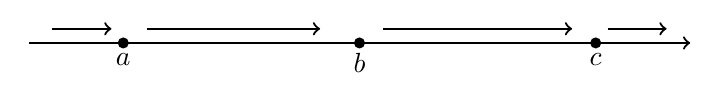
\begin{tikzpicture}[x=1cm,y=1cm,thick]
  \draw[->] (-4.2,0)--(4.2,0);
  \foreach \x/\lab in {-3/a,0/b,3/c} {\fill (\x,0) circle (2pt); \node[below] at (\x,0) {$\lab$};}
  \foreach \a/\b in {-2.7/-0.5,0.3/2.7} {\draw[->] (\a,0.18)--(\b,0.18);}
  \draw[->] (-3.9,0.18)--(-3.15,0.18); \draw[->] (3.15,0.18)--(3.9,0.18);
\end{tikzpicture}

 \caption{原书图 17：直线上各相邻平衡位置把相空间分成互不相交的区间；箭头表示当
 \(f>0\) 时轨线随 \(t\) 增大而向右运动，因此每个开区间都是一条单独的相轨线。}
 \label{fig:ch2-p2-17}
\end{figure}

证明先把 \(f(x_0)>0\) 局部化为 \(f>0\) 在 \((a,b)\) 上恒成立。只要 \(\varphi(t)\)
仍在 \((a,b)\) 中，它就只能从左向右运动；若在某个有限时刻越出右端点 \(b\)，就会与另一
条轨线 \(x=b\) 在有限时刻相遇，违反唯一性。左端同理。因此点不能在内部越界。

再证明极限达到相邻零点。假设
\(\lim_{t\to r_2}\varphi(t)=c\)，其中 \(c<b\)。取初值为 \(c\) 的另一条解。
因为 \(f(c)>0\)，该解在某个较早时刻会经过 \(c\) 的值，而 \(c\) 不属于原轨线的取值
范围，于是两条轨线相交，矛盾。因此只能有 \(\lim_{t\to r_2}\varphi(t)=b\)。左端
\(\lim_{t\to r_1}\varphi(t)=a\) 同理。最后，若 \(b<+\infty\) 而 \(r_2<+\infty\)，
把解在 \(r_2\) 之后接成常值 \(b\)，就会得到经过 \(b\) 的另一条解，也违反唯一性。
所以有限端点对应的存在时间必须是无穷。对左端点作同样论证。

现在设 \(b\) 是方程 \(x'=f(x)\) 的平衡位置，而 \((a,b)\) 与 \((b,c)\) 是左右相邻的
两个区间。如果当 \(t\) 增大时，两个相邻区间中的点都趋近于 \(b\)，就称 \(b\) 为稳定平衡
位置，见图~\ref{fig:ch2-p2-18}(a)。如果两边都离开 \(b\)，称它为不稳定的，见图
\ref{fig:ch2-p2-18}(b)。如果一边趋近而另一边离开，称它为半稳定的，见图
\ref{fig:ch2-p2-18}(c)。

\begin{figure}[H]
 \centering
 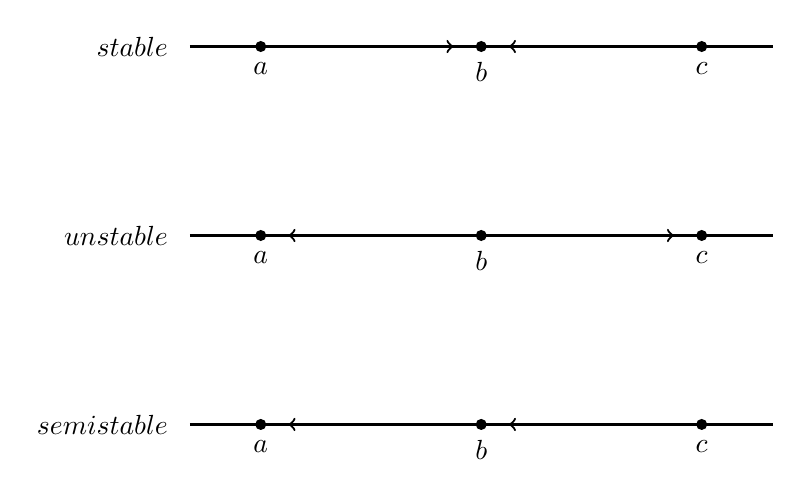
\begin{tikzpicture}[x=1cm,y=1cm,thick]
  % The three rows show the two intervals adjacent to b.
  \foreach \y/\case in {2.4/stable,0/unstable,-2.4/semistable} {
    \draw (-3.7,\y)--(3.7,\y);
    \foreach \x/\lab in {-2.8/a,0/b,2.8/c} {
      \fill (\x,\y) circle (2pt);
      \node[below=2pt] at (\x,\y) {$\lab$};
    }
    \node[left] at (-3.85,\y) {$\case$};
  }
  % Stable: both neighboring intervals flow toward b.
  \draw[->] (-2.45,2.4)--(-0.35,2.4);
  \draw[->] (2.45,2.4)--(0.35,2.4);
  % Unstable: both intervals flow away from b.
  \draw[<-] (-2.45,0)--(-0.35,0);
  \draw[->] (0.35,0)--(2.45,0);
  % Semistable: the left side leaves b while the right side approaches it.
  \draw[<-] (-2.45,-2.4)--(-0.35,-2.4);
  \draw[->] (2.45,-2.4)--(0.35,-2.4);
\end{tikzpicture}

 \caption{原书图 18：上、中、下三行分别表示稳定、不稳定和半稳定平衡位置。左右区间上
 的箭头由 \(f\) 的符号决定：指向 \(b\) 表示趋近，背离 \(b\) 表示离开；三个零点分别
 是 \(a,b,c\)。}
 \label{fig:ch2-p2-18}
\end{figure}

用函数符号判断，平衡位置 \(b\) 稳定，当且仅当 \(f\) 在 \((a,b)\) 上为正、在
\((b,c)\) 上为负；不稳定，当且仅当 \(f\) 在左侧为负、在右侧为正；半稳定，当且仅当
两侧同号。若 \(f'(b)\neq0\)，在 \(b\) 附近 \(f(x)\) 的符号与 \(f'(b)(x-b)\) 一致。
于是 \(f'(b)<0\) 时 \(b\) 稳定，\(f'(b)>0\) 时不稳定。若 \(f'(b)=0\)，一阶导数不能
给出结论，必须检查更高阶项或直接看左右符号。

\paragraph{例 2.}
考察方程
\begin{equation}
 x'=f(x),
 \tag{19}
\end{equation}
其中 \(f\) 是以 \(2\pi\) 为周期的连续可微函数：
\[
 f(x+2k\pi)=f(x),\qquad k\in\mathbb Z.
\]
例 1 的局部结论仍适用于每个标量解，但由于 \(f\) 的周期性，把相空间看成半径为 \(1\) 的
圆周 \(K\) 更合适。固定圆周上的计算起点 \(O\) 和逆时针方向；在圆周上取从 \(O\) 沿逆时针
方向弧长为 \(x\) 的点 \(\xi\)，再把所有实数 \(x\) 对应到 \(K\) 上的点。于是 \(x\) 与
\(x+2k\pi\) 对应同一个 \(\xi\)。因为 \(f\) 有相同周期，可以令
\[
 f(\xi)=f(x)
\]
把 \(f\) 看成定义在圆周 \(K\) 上的函数。

方程 \(x'=f(x)\) 于是描述了点在圆周上的运动。若 \(x(t)\) 是一个解，则对应的点
\(\xi(t)\) 沿圆周运动。若 \(\alpha\in K\) 满足 \(f(\alpha)=0\)，则 \(\xi=\alpha\)
是平衡位置。为简单起见，假设圆周上的平衡位置没有极限点，于是平衡位置只能有有限多个
或者一个也没有。平衡位置把圆周分成若干个区间；若没有平衡位置，整个圆周就是一个区间；
若恰有一个平衡位置 \(\alpha\)，则圆周去掉 \(\alpha\) 后也只有一个区间，其两个端点实际
上重合。

\begin{figure}[H]
 \centering
 \begin{tikzpicture}[x=1cm,y=1cm,thick,>=Stealth]
  \def\radius{1.8}
  % The full phase space is a circle; x is measured along its circumference.
  \draw[dashed] (0,0) circle (\radius);
  \draw[->,very thick]
    (\radius,0) arc[start angle=0,end angle=62,radius=\radius]
    node[midway,above right] {$x$};
  \fill (\radius,0) circle (2pt) node[right=3pt] {$O$};
  \fill ({\radius*cos(62)},{\radius*sin(62)}) circle (2pt)
    node[above right=2pt] {$\xi$};
  \node at (0,2.18) {$K$};
\end{tikzpicture}

 \caption{原书图 19：周期函数的相空间。圆周 \(K\) 上没有直角坐标轴，起点 \(O\)
 用来量弧长；实数 \(x\) 对应弧长 \(x\) 的点 \(\xi\)，\(x\) 与 \(x+2k\pi\) 落在
 同一点。参数条件是 \(f\) 以 \(2\pi\) 为周期。}
 \label{fig:ch2-p2-19}
\end{figure}

\begin{figure}[H]
 \centering
 \begin{tikzpicture}[scale=2.3542,font=\small,x=1cm,y=1cm,line width=0.8pt]
  % Six equilibria: three sinks alternate with three sources on the circle.
  \draw (0,0) circle (2);
  \foreach \ang in {0,76,132,213,256,286}
    \fill ({2*cos(\ang)},{2*sin(\ang)}) circle (1.6pt);
  \foreach \a/\b in {15/4,-15/-4,117/128,147/136,241/252,271/260}
    \draw[->] ({2*cos(\a)},{2*sin(\a)})
      arc[start angle=\a,end angle=\b,radius=2];
\end{tikzpicture}

 \caption{原书图 20：圆周 \(K\) 上的平衡点把圆周切成带方向的弧段。箭头显示各弧段内
 \(f\) 的符号所确定的运动方向；若没有平衡点，整圆是一条周期轨线，若只有一个平衡点，
 圆周去掉该点后仍是一条带有重合端点的轨线。}
 \label{fig:ch2-p2-20}
\end{figure}

取区间 \(I\) 中一点 \(\xi_0\)，设 \(x(t)\) 是以 \(x(0)=x_0\) 为初值的标量解，而
\(\xi(t)\) 是对应圆周上的点。若区间有端点，点沿确定方向运动，除端点外每一点都由轨线
经过一次。若区间就是整个圆周，则从位置 \(\xi_0\) 出发的点经过某段时间 \(T\) 回到
\(\xi_0\)，所以
\[
 \xi(0)=\xi(T).
\]
对应到原来的实变量 \(x(t)\)，有
\[
 x(t+T)=x(t)\pm2\pi,
\]
正负号由绕行方向决定。这个例子说明相空间不一定是欧氏坐标空间，可以是一个圆周；轨线的
几何形状必须与函数展开的周期性一起理解。

\paragraph{例 3.}
考虑平面周期系统
\begin{equation}
 x_i'=f_i(x_1,x_2),\qquad i=1,2,
 \tag{20}
\end{equation}
其中 \(f_i\) 连续可微，并有周期
\[
 f_i(x_1+2k\pi,x_2+2l\pi)=f_i(x_1,x_2),\qquad k,l\in\mathbb Z.
\]
此时把相空间看成环面最合适。在三维欧氏空间的 \((x,z)\) 平面中取圆心为 \((2,0,0)\)、
半径为 \(1\) 的圆 \(K\)。取点 \((3,0,0)\) 为计算起点。对每个 \(x_1\)，按例 2 的弧长
规则在 \(K\) 上取点 \(\xi_1\)。再绕 \(z\) 轴旋转 \((x,z)\) 平面，旋转角为 \(x_2\)；
圆 \(K\) 旋转所描出的曲面就是环面。若旋转角由 \(x_2\) 增加到 \(x_2+2\pi\)，平面回到
自身，环面上的点也回到同一点。因此环面上的一点由两个循环坐标 \((\xi_1,\xi_2)\)
完全确定，而每一对循环坐标唯一确定一点。

\begin{figure}[H]
 \centering
 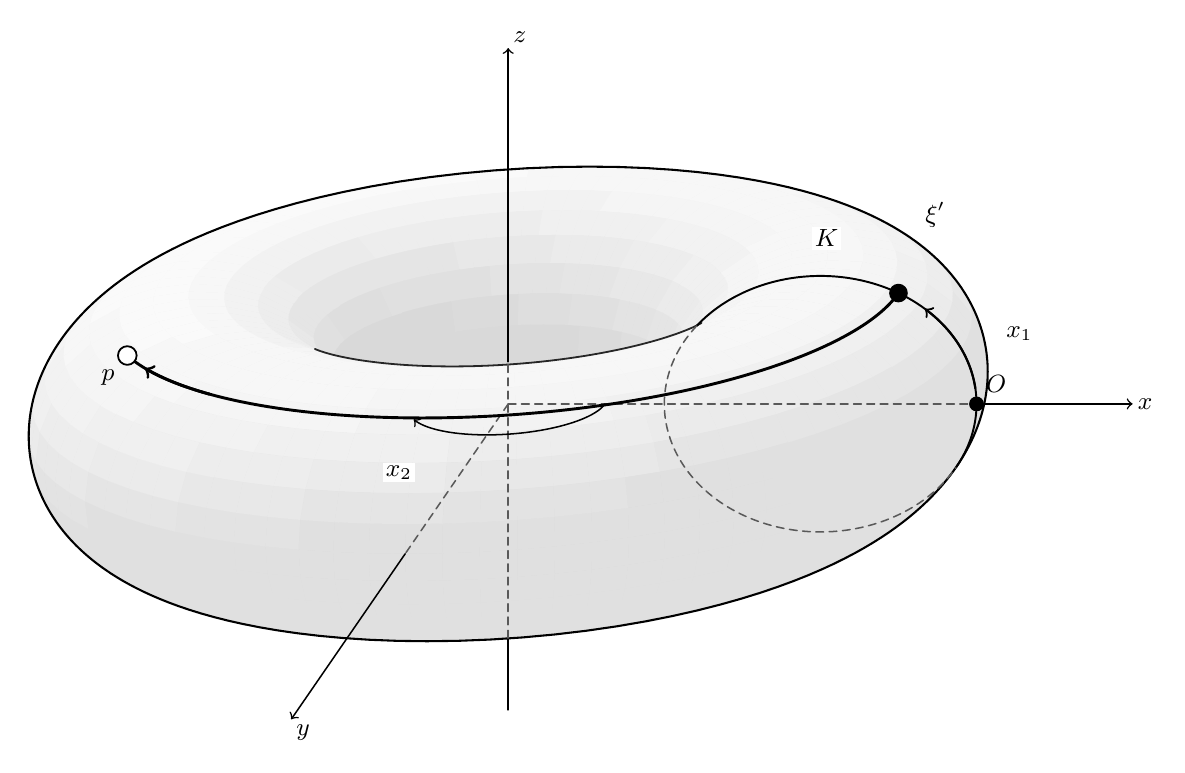
\begin{tikzpicture}[scale=1.9825,font=\small,x=1cm,y=1cm,line cap=round,line join=round,
  every node/.style={font=\small,inner sep=1.6pt},
  axis/.style={line width=.55pt},
  hidden/.style={line width=.55pt,dash pattern=on 2.8pt off 2pt,black!65}]
% Parametric torus ((2+cos v)cos u,(2+cos v)sin u,sin v).
% One consistent oblique projection: (X,Y)=(x-.22y,.82z-.32y).
% The small solid patches below are depth-sorted surface facets, not separate ellipses.
% They provide only a pale wash; the exact smooth contour is drawn afterwards.
  \path[fill=black!12,draw=black!12,line width=.10pt] (-0.0566,0.5469) -- (0.1765,0.5611) -- (0.1810,0.7578) -- (-0.0581,0.7432) -- cycle;
  \path[fill=black!12,draw=black!12,line width=.10pt] (-0.2895,0.5271) -- (-0.0566,0.5469) -- (-0.0581,0.7432) -- (-0.2969,0.7229) -- cycle;
  \path[fill=black!12,draw=black!12,line width=.10pt] (0.1765,0.5611) -- (0.4086,0.5697) -- (0.4191,0.7666) -- (0.1810,0.7578) -- cycle;
  \path[fill=black!12,draw=black!12,line width=.10pt] (-0.0543,0.3543) -- (0.1693,0.3680) -- (0.1765,0.5611) -- (-0.0566,0.5469) -- cycle;
  \path[fill=black!12,draw=black!12,line width=.10pt] (-0.2776,0.3354) -- (-0.0543,0.3543) -- (-0.0566,0.5469) -- (-0.2895,0.5271) -- cycle;
  \path[fill=black!12,draw=black!12,line width=.10pt] (-0.5205,0.5019) -- (-0.2895,0.5271) -- (-0.2969,0.7229) -- (-0.5338,0.6970) -- cycle;
  \path[fill=black!11,draw=black!11,line width=.10pt] (-0.0581,0.7432) -- (0.1810,0.7578) -- (0.1826,0.9482) -- (-0.0586,0.9335) -- cycle;
  \path[fill=black!12,draw=black!12,line width=.10pt] (0.1693,0.3680) -- (0.3919,0.3762) -- (0.4086,0.5697) -- (0.1765,0.5611) -- cycle;
  \path[fill=black!11,draw=black!11,line width=.10pt] (-0.2969,0.7229) -- (-0.0581,0.7432) -- (-0.0586,0.9335) -- (-0.2994,0.9130) -- cycle;
  \path[fill=black!12,draw=black!12,line width=.10pt] (0.4086,0.5697) -- (0.6382,0.5725) -- (0.6545,0.7695) -- (0.4191,0.7666) -- cycle;
  \path[fill=black!12,draw=black!12,line width=.10pt] (-0.4991,0.3112) -- (-0.2776,0.3354) -- (-0.2895,0.5271) -- (-0.5205,0.5019) -- cycle;
  \path[fill=black!11,draw=black!11,line width=.10pt] (0.1810,0.7578) -- (0.4191,0.7666) -- (0.4226,0.9570) -- (0.1826,0.9482) -- cycle;
  \path[fill=black!11,draw=black!11,line width=.10pt] (-0.5338,0.6970) -- (-0.2969,0.7229) -- (-0.2994,0.9130) -- (-0.5383,0.8869) -- cycle;
  \path[fill=black!12,draw=black!12,line width=.10pt] (0.3919,0.3762) -- (0.6120,0.3789) -- (0.6382,0.5725) -- (0.4086,0.5697) -- cycle;
  \path[fill=black!12,draw=black!12,line width=.10pt] (-0.7484,0.4713) -- (-0.5205,0.5019) -- (-0.5338,0.6970) -- (-0.7674,0.6658) -- cycle;
  \path[fill=black!12,draw=black!12,line width=.10pt] (0.4191,0.7666) -- (0.6545,0.7695) -- (0.6600,0.9600) -- (0.4226,0.9570) -- cycle;
  \path[fill=black!12,draw=black!12,line width=.10pt] (-0.7176,0.2819) -- (-0.4991,0.3112) -- (-0.5205,0.5019) -- (-0.7484,0.4713) -- cycle;
  \path[fill=black!12,draw=black!12,line width=.10pt] (-0.0512,0.1752) -- (0.1597,0.1881) -- (0.1693,0.3680) -- (-0.0543,0.3543) -- cycle;
  \path[fill=black!12,draw=black!12,line width=.10pt] (0.6382,0.5725) -- (0.8639,0.5697) -- (0.8859,0.7666) -- (0.6545,0.7695) -- cycle;
  \path[fill=black!12,draw=black!12,line width=.10pt] (-0.2618,0.1573) -- (-0.0512,0.1752) -- (-0.0543,0.3543) -- (-0.2776,0.3354) -- cycle;
  \path[fill=black!10,draw=black!10,line width=.10pt] (-0.7674,0.6658) -- (-0.5338,0.6970) -- (-0.5383,0.8869) -- (-0.7739,0.8554) -- cycle;
  \path[fill=black!12,draw=black!12,line width=.10pt] (0.1597,0.1881) -- (0.3696,0.1958) -- (0.3919,0.3762) -- (0.1693,0.3680) -- cycle;
  \path[fill=black!12,draw=black!12,line width=.10pt] (0.6120,0.3789) -- (0.8284,0.3762) -- (0.8639,0.5697) -- (0.6382,0.5725) -- cycle;
  \path[fill=black!12,draw=black!12,line width=.10pt] (-0.4707,0.1345) -- (-0.2618,0.1573) -- (-0.2776,0.3354) -- (-0.4991,0.3112) -- cycle;
  \path[fill=black!9,draw=black!9,line width=.10pt] (-0.0586,0.9335) -- (0.1826,0.9482) -- (0.1810,1.1227) -- (-0.0581,1.1081) -- cycle;
  \path[fill=black!9,draw=black!9,line width=.10pt] (-0.2994,0.9130) -- (-0.0586,0.9335) -- (-0.0581,1.1081) -- (-0.2969,1.0879) -- cycle;
  \path[fill=black!12,draw=black!12,line width=.10pt] (-0.9716,0.4357) -- (-0.7484,0.4713) -- (-0.7674,0.6658) -- (-0.9964,0.6292) -- cycle;
  \path[fill=black!12,draw=black!12,line width=.10pt] (0.6545,0.7695) -- (0.8859,0.7666) -- (0.8933,0.9570) -- (0.6600,0.9600) -- cycle;
  \path[fill=black!9,draw=black!9,line width=.10pt] (0.1826,0.9482) -- (0.4226,0.9570) -- (0.4191,1.1315) -- (0.1810,1.1227) -- cycle;
  \path[fill=black!12,draw=black!12,line width=.10pt] (0.3696,0.1958) -- (0.5772,0.1984) -- (0.6120,0.3789) -- (0.3919,0.3762) -- cycle;
  \path[fill=black!12,draw=black!12,line width=.10pt] (-0.9317,0.2477) -- (-0.7176,0.2819) -- (-0.7484,0.4713) -- (-0.9716,0.4357) -- cycle;
  \path[fill=black!9,draw=black!9,line width=.10pt] (-0.5383,0.8869) -- (-0.2994,0.9130) -- (-0.2969,1.0879) -- (-0.5338,1.0620) -- cycle;
  \path[fill=black!12,draw=black!12,line width=.10pt] (-0.6768,0.1069) -- (-0.4707,0.1345) -- (-0.4991,0.3112) -- (-0.7176,0.2819) -- cycle;
  \path[fill=black!10,draw=black!10,line width=.10pt] (-0.9964,0.6292) -- (-0.7674,0.6658) -- (-0.7739,0.8554) -- (-1.0048,0.8185) -- cycle;
  \path[fill=black!12,draw=black!12,line width=.10pt] (0.8639,0.5697) -- (1.0842,0.5611) -- (1.1118,0.7578) -- (0.8859,0.7666) -- cycle;
  \path[fill=black!9,draw=black!9,line width=.10pt] (0.4226,0.9570) -- (0.6600,0.9600) -- (0.6545,1.1344) -- (0.4191,1.1315) -- cycle;
  \path[fill=black!12,draw=black!12,line width=.10pt] (0.8284,0.3762) -- (1.0396,0.3680) -- (1.0842,0.5611) -- (0.8639,0.5697) -- cycle;
  \path[fill=black!12,draw=black!12,line width=.10pt] (0.5772,0.1984) -- (0.7812,0.1958) -- (0.8284,0.3762) -- (0.6120,0.3789) -- cycle;
  \path[fill=black!8,draw=black!8,line width=.10pt] (-0.7739,0.8554) -- (-0.5383,0.8869) -- (-0.5338,1.0620) -- (-0.7674,1.0307) -- cycle;
  \path[fill=black!12,draw=black!12,line width=.10pt] (0.8859,0.7666) -- (1.1118,0.7578) -- (1.1212,0.9482) -- (0.8933,0.9570) -- cycle;
  \path[fill=black!12,draw=black!12,line width=.10pt] (-1.1888,0.3952) -- (-0.9716,0.4357) -- (-0.9964,0.6292) -- (-1.2191,0.5877) -- cycle;
  \path[fill=black!12,draw=black!12,line width=.10pt] (-0.8787,0.0747) -- (-0.6768,0.1069) -- (-0.7176,0.2819) -- (-0.9317,0.2477) -- cycle;
  \path[fill=black!12,draw=black!12,line width=.10pt] (-1.1400,0.2089) -- (-0.9317,0.2477) -- (-0.9716,0.4357) -- (-1.1888,0.3952) -- cycle;
  \path[fill=black!12,draw=black!12,line width=.10pt] (-0.0475,0.0185) -- (0.1481,0.0305) -- (0.1597,0.1881) -- (-0.0512,0.1752) -- cycle;
  \path[fill=black!10,draw=black!10,line width=.10pt] (0.6600,0.9600) -- (0.8933,0.9570) -- (0.8859,1.1315) -- (0.6545,1.1344) -- cycle;
  \path[fill=black!12,draw=black!12,line width=.10pt] (-0.2429,0.0019) -- (-0.0475,0.0185) -- (-0.0512,0.1752) -- (-0.2618,0.1573) -- cycle;
  \path[fill=black!12,draw=black!12,line width=.10pt] (0.1481,0.0305) -- (0.3428,0.0376) -- (0.3696,0.1958) -- (0.1597,0.1881) -- cycle;
  \path[fill=black!10,draw=black!10,line width=.10pt] (-1.2191,0.5877) -- (-0.9964,0.6292) -- (-1.0048,0.8185) -- (-1.2294,0.7767) -- cycle;
  \path[fill=black!12,draw=black!12,line width=.10pt] (-0.4367,-0.0192) -- (-0.2429,0.0019) -- (-0.2618,0.1573) -- (-0.4707,0.1345) -- cycle;
  \path[fill=black!12,draw=black!12,line width=.10pt] (0.7812,0.1958) -- (0.9805,0.1881) -- (1.0396,0.3680) -- (0.8284,0.3762) -- cycle;
  \path[fill=black!8,draw=black!8,line width=.10pt] (-1.0048,0.8185) -- (-0.7739,0.8554) -- (-0.7674,1.0307) -- (-0.9964,0.9942) -- cycle;
  \path[fill=black!12,draw=black!12,line width=.10pt] (1.0842,0.5611) -- (1.2978,0.5469) -- (1.3309,0.7432) -- (1.1118,0.7578) -- cycle;
  \path[fill=black!7,draw=black!7,line width=.10pt] (-0.0581,1.1081) -- (0.1810,1.1227) -- (0.1765,1.2727) -- (-0.0566,1.2584) -- cycle;
  \path[fill=black!12,draw=black!12,line width=.10pt] (0.3428,0.0376) -- (0.5355,0.0400) -- (0.5772,0.1984) -- (0.3696,0.1958) -- cycle;
  \path[fill=black!7,draw=black!7,line width=.10pt] (-0.2969,1.0879) -- (-0.0581,1.1081) -- (-0.0566,1.2584) -- (-0.2895,1.2387) -- cycle;
  \path[fill=black!12,draw=black!12,line width=.10pt] (1.0396,0.3680) -- (1.2445,0.3543) -- (1.2978,0.5469) -- (1.0842,0.5611) -- cycle;
  \path[fill=black!7,draw=black!7,line width=.10pt] (0.1810,1.1227) -- (0.4191,1.1315) -- (0.4086,1.2812) -- (0.1765,1.2727) -- cycle;
  \path[fill=black!12,draw=black!12,line width=.10pt] (-0.6279,-0.0448) -- (-0.4367,-0.0192) -- (-0.4707,0.1345) -- (-0.6768,0.1069) -- cycle;
  \path[fill=black!12,draw=black!12,line width=.10pt] (-1.0751,0.0381) -- (-0.8787,0.0747) -- (-0.9317,0.2477) -- (-1.1400,0.2089) -- cycle;
  \path[fill=black!7,draw=black!7,line width=.10pt] (-0.5338,1.0620) -- (-0.2969,1.0879) -- (-0.2895,1.2387) -- (-0.5205,1.2134) -- cycle;
  \path[fill=black!10,draw=black!10,line width=.10pt] (0.8933,0.9570) -- (1.1212,0.9482) -- (1.1118,1.1227) -- (0.8859,1.1315) -- cycle;
  \path[fill=black!12,draw=black!12,line width=.10pt] (1.1118,0.7578) -- (1.3309,0.7432) -- (1.3421,0.9335) -- (1.1212,0.9482) -- cycle;
  \path[fill=black!12,draw=black!12,line width=.10pt] (-1.3987,0.3501) -- (-1.1888,0.3952) -- (-1.2191,0.5877) -- (-1.4344,0.5414) -- cycle;
  \path[fill=black!12,draw=black!12,line width=.10pt] (0.5355,0.0400) -- (0.7248,0.0376) -- (0.7812,0.1958) -- (0.5772,0.1984) -- cycle;
  \path[fill=black!7,draw=black!7,line width=.10pt] (0.4191,1.1315) -- (0.6545,1.1344) -- (0.6382,1.2841) -- (0.4086,1.2812) -- cycle;
  \path[fill=black!12,draw=black!12,line width=.10pt] (-1.3413,0.1656) -- (-1.1400,0.2089) -- (-1.1888,0.3952) -- (-1.3987,0.3501) -- cycle;
  \path[fill=black!6,draw=black!6,line width=.10pt] (-0.7674,1.0307) -- (-0.5338,1.0620) -- (-0.5205,1.2134) -- (-0.7484,1.1829) -- cycle;
  \path[fill=black!12,draw=black!12,line width=.10pt] (0.9805,0.1881) -- (1.1737,0.1752) -- (1.2445,0.3543) -- (1.0396,0.3680) -- cycle;
  \path[fill=black!12,draw=black!12,line width=.10pt] (-0.8152,-0.0747) -- (-0.6279,-0.0448) -- (-0.6768,0.1069) -- (-0.8787,0.0747) -- cycle;
  \path[fill=black!8,draw=black!8,line width=.10pt] (-1.2294,0.7767) -- (-1.0048,0.8185) -- (-0.9964,0.9942) -- (-1.2191,0.9526) -- cycle;
  \path[fill=black!10,draw=black!10,line width=.10pt] (-1.4344,0.5414) -- (-1.2191,0.5877) -- (-1.2294,0.7767) -- (-1.4465,0.7300) -- cycle;
  \path[fill=black!8,draw=black!8,line width=.10pt] (0.6545,1.1344) -- (0.8859,1.1315) -- (0.8639,1.2812) -- (0.6382,1.2841) -- cycle;
  \path[fill=black!12,draw=black!12,line width=.10pt] (1.2978,0.5469) -- (1.5034,0.5271) -- (1.5418,0.7229) -- (1.3309,0.7432) -- cycle;
  \path[fill=black!12,draw=black!12,line width=.10pt] (0.7248,0.0376) -- (0.9096,0.0305) -- (0.9805,0.1881) -- (0.7812,0.1958) -- cycle;
  \path[fill=black!12,draw=black!12,line width=.10pt] (1.2445,0.3543) -- (1.4417,0.3354) -- (1.5034,0.5271) -- (1.2978,0.5469) -- cycle;
  \path[fill=black!12,draw=black!12,line width=.10pt] (-1.2649,-0.0027) -- (-1.0751,0.0381) -- (-1.1400,0.2089) -- (-1.3413,0.1656) -- cycle;
  \path[fill=black!10,draw=black!10,line width=.10pt] (1.1212,0.9482) -- (1.3421,0.9335) -- (1.3309,1.1081) -- (1.1118,1.1227) -- cycle;
  \path[fill=black!6,draw=black!6,line width=.10pt] (-0.9964,0.9942) -- (-0.7674,1.0307) -- (-0.7484,1.1829) -- (-0.9716,1.1473) -- cycle;
  \path[fill=black!12,draw=black!12,line width=.10pt] (-0.0434,-0.1079) -- (0.1353,-0.0970) -- (0.1481,0.0305) -- (-0.0475,0.0185) -- cycle;
  \path[fill=black!12,draw=black!12,line width=.10pt] (-0.2218,-0.1230) -- (-0.0434,-0.1079) -- (-0.0475,0.0185) -- (-0.2429,0.0019) -- cycle;
  \path[fill=black!12,draw=black!12,line width=.10pt] (1.3309,0.7432) -- (1.5418,0.7229) -- (1.5547,0.9130) -- (1.3421,0.9335) -- cycle;
  \path[fill=black!12,draw=black!12,line width=.10pt] (-0.9974,-0.1087) -- (-0.8152,-0.0747) -- (-0.8787,0.0747) -- (-1.0751,0.0381) -- cycle;
  \path[fill=black!12,draw=black!12,line width=.10pt] (0.1353,-0.0970) -- (0.3131,-0.0904) -- (0.3428,0.0376) -- (0.1481,0.0305) -- cycle;
  \path[fill=black!12,draw=black!12,line width=.10pt] (-0.3988,-0.1424) -- (-0.2218,-0.1230) -- (-0.2429,0.0019) -- (-0.4367,-0.0192) -- cycle;
  \path[fill=black!12,draw=black!12,line width=.10pt] (-1.6000,0.3006) -- (-1.3987,0.3501) -- (-1.4344,0.5414) -- (-1.6408,0.4907) -- cycle;
  \path[fill=black!12,draw=black!12,line width=.10pt] (-1.5343,0.1182) -- (-1.3413,0.1656) -- (-1.3987,0.3501) -- (-1.6000,0.3006) -- cycle;
  \path[fill=black!12,draw=black!12,line width=.10pt] (1.1737,0.1752) -- (1.3596,0.1573) -- (1.4417,0.3354) -- (1.2445,0.3543) -- cycle;
  \path[fill=black!8,draw=black!8,line width=.10pt] (0.8859,1.1315) -- (1.1118,1.1227) -- (1.0842,1.2727) -- (0.8639,1.2812) -- cycle;
  \path[fill=black!12,draw=black!12,line width=.10pt] (0.3131,-0.0904) -- (0.4890,-0.0882) -- (0.5355,0.0400) -- (0.3428,0.0376) -- cycle;
  \path[fill=black!8,draw=black!8,line width=.10pt] (-1.4465,0.7300) -- (-1.2294,0.7767) -- (-1.2191,0.9526) -- (-1.4344,0.9064) -- cycle;
  \path[fill=black!5,draw=black!5,line width=.10pt] (-0.0566,1.2584) -- (0.1765,1.2727) -- (0.1693,1.3905) -- (-0.0543,1.3769) -- cycle;
  \path[fill=black!12,draw=black!12,line width=.10pt] (0.9096,0.0305) -- (1.0888,0.0185) -- (1.1737,0.1752) -- (0.9805,0.1881) -- cycle;
  \path[fill=black!5,draw=black!5,line width=.10pt] (-0.2895,1.2387) -- (-0.0566,1.2584) -- (-0.0543,1.3769) -- (-0.2776,1.3579) -- cycle;
  \path[fill=black!12,draw=black!12,line width=.10pt] (-0.5733,-0.1658) -- (-0.3988,-0.1424) -- (-0.4367,-0.0192) -- (-0.6279,-0.0448) -- cycle;
  \path[fill=black!6,draw=black!6,line width=.10pt] (0.1765,1.2727) -- (0.4086,1.2812) -- (0.3919,1.3987) -- (0.1693,1.3905) -- cycle;
  \path[fill=black!10,draw=black!10,line width=.10pt] (-1.6408,0.4907) -- (-1.4344,0.5414) -- (-1.4465,0.7300) -- (-1.6546,0.6788) -- cycle;
  \path[fill=black!5,draw=black!5,line width=.10pt] (-0.5205,1.2134) -- (-0.2895,1.2387) -- (-0.2776,1.3579) -- (-0.4991,1.3337) -- cycle;
  \path[fill=black!6,draw=black!6,line width=.10pt] (-1.2191,0.9526) -- (-0.9964,0.9942) -- (-0.9716,1.1473) -- (-1.1888,1.1068) -- cycle;
  \path[fill=black!12,draw=black!12,line width=.10pt] (0.4890,-0.0882) -- (0.6618,-0.0904) -- (0.7248,0.0376) -- (0.5355,0.0400) -- cycle;
  \path[fill=black!12,draw=black!12,line width=.10pt] (-1.4470,-0.0475) -- (-1.2649,-0.0027) -- (-1.3413,0.1656) -- (-1.5343,0.1182) -- cycle;
  \path[fill=black!12,draw=black!12,line width=.10pt] (1.5034,0.5271) -- (1.6998,0.5019) -- (1.7431,0.6970) -- (1.5418,0.7229) -- cycle;
  \path[fill=black!12,draw=black!12,line width=.10pt] (-1.1735,-0.1466) -- (-0.9974,-0.1087) -- (-1.0751,0.0381) -- (-1.2649,-0.0027) -- cycle;
  \path[fill=black!12,draw=black!12,line width=.10pt] (1.4417,0.3354) -- (1.6300,0.3112) -- (1.6998,0.5019) -- (1.5034,0.5271) -- cycle;
  \path[fill=black!6,draw=black!6,line width=.10pt] (0.4086,1.2812) -- (0.6382,1.2841) -- (0.6120,1.4014) -- (0.3919,1.3987) -- cycle;
  \path[fill=black!10,draw=black!10,line width=.10pt] (1.3421,0.9335) -- (1.5547,0.9130) -- (1.5418,1.0879) -- (1.3309,1.1081) -- cycle;
  \path[fill=black!12,draw=black!12,line width=.10pt] (-0.7444,-0.1930) -- (-0.5733,-0.1658) -- (-0.6279,-0.0448) -- (-0.8152,-0.0747) -- cycle;
  \path[fill=black!5,draw=black!5,line width=.10pt] (-0.7484,1.1829) -- (-0.5205,1.2134) -- (-0.4991,1.3337) -- (-0.7176,1.3044) -- cycle;
  \path[fill=black!8,draw=black!8,line width=.10pt] (1.1118,1.1227) -- (1.3309,1.1081) -- (1.2978,1.2584) -- (1.0842,1.2727) -- cycle;
  \path[fill=black!12,draw=black!12,line width=.10pt] (1.5418,0.7229) -- (1.7431,0.6970) -- (1.7578,0.8869) -- (1.5547,0.9130) -- cycle;
  \path[fill=black!12,draw=black!12,line width=.10pt] (0.6618,-0.0904) -- (0.8306,-0.0970) -- (0.9096,0.0305) -- (0.7248,0.0376) -- cycle;
  \path[fill=black!12,draw=black!12,line width=.10pt] (1.0888,0.0185) -- (1.2614,0.0019) -- (1.3596,0.1573) -- (1.1737,0.1752) -- cycle;
  \path[fill=black!6,draw=black!6,line width=.10pt] (0.6382,1.2841) -- (0.8639,1.2812) -- (0.8284,1.3987) -- (0.6120,1.4014) -- cycle;
  \path[fill=black!12,draw=black!12,line width=.10pt] (1.3596,0.1573) -- (1.5372,0.1345) -- (1.6300,0.3112) -- (1.4417,0.3354) -- cycle;
  \path[fill=black!12,draw=black!12,line width=.10pt] (-1.7914,0.2471) -- (-1.6000,0.3006) -- (-1.6408,0.4907) -- (-1.8371,0.4358) -- cycle;
  \path[fill=black!8,draw=black!8,line width=.10pt] (-1.6546,0.6788) -- (-1.4465,0.7300) -- (-1.4344,0.9064) -- (-1.6408,0.8556) -- cycle;
  \path[fill=black!12,draw=black!12,line width=.10pt] (-1.7179,0.0669) -- (-1.5343,0.1182) -- (-1.6000,0.3006) -- (-1.7914,0.2471) -- cycle;
  \path[fill=black!12,draw=black!12,line width=.10pt] (-0.9108,-0.2241) -- (-0.7444,-0.1930) -- (-0.8152,-0.0747) -- (-0.9974,-0.1087) -- cycle;
  \path[fill=black!6,draw=black!6,line width=.10pt] (-1.4344,0.9064) -- (-1.2191,0.9526) -- (-1.1888,1.1068) -- (-1.3987,1.0617) -- cycle;
  \path[fill=black!5,draw=black!5,line width=.10pt] (-0.9716,1.1473) -- (-0.7484,1.1829) -- (-0.7176,1.3044) -- (-0.9317,1.2703) -- cycle;
  \path[fill=black!12,draw=black!12,line width=.10pt] (-1.3424,-0.1881) -- (-1.1735,-0.1466) -- (-1.2649,-0.0027) -- (-1.4470,-0.0475) -- cycle;
  \path[fill=black!10,draw=black!10,line width=.10pt] (-1.8371,0.4358) -- (-1.6408,0.4907) -- (-1.6546,0.6788) -- (-1.8526,0.6235) -- cycle;
  \path[fill=black!12,draw=black!12,line width=.10pt] (0.8306,-0.0970) -- (0.9943,-0.1079) -- (1.0888,0.0185) -- (0.9096,0.0305) -- cycle;
  \path[fill=black!12,draw=black!12,line width=.10pt] (-1.6201,-0.0959) -- (-1.4470,-0.0475) -- (-1.5343,0.1182) -- (-1.7179,0.0669) -- cycle;
  \path[fill=black!12,draw=black!12,line width=.10pt] (-0.0390,-0.1977) -- (0.1217,-0.1879) -- (0.1353,-0.0970) -- (-0.0434,-0.1079) -- cycle;
  \path[fill=black!12,draw=black!12,line width=.10pt] (-0.1996,-0.2113) -- (-0.0390,-0.1977) -- (-0.0434,-0.1079) -- (-0.2218,-0.1230) -- cycle;
  \path[fill=black!6,draw=black!6,line width=.10pt] (0.8639,1.2812) -- (1.0842,1.2727) -- (1.0396,1.3905) -- (0.8284,1.3987) -- cycle;
  \path[fill=black!12,draw=black!12,line width=.10pt] (0.1217,-0.1879) -- (0.2817,-0.1820) -- (0.3131,-0.0904) -- (0.1353,-0.0970) -- cycle;
  \path[fill=black!11,draw=black!11,line width=.10pt] (1.5547,0.9130) -- (1.7578,0.8869) -- (1.7431,1.0620) -- (1.5418,1.0879) -- cycle;
  \path[fill=black!12,draw=black!12,line width=.10pt] (1.6998,0.5019) -- (1.8857,0.4713) -- (1.9337,0.6658) -- (1.7431,0.6970) -- cycle;
  \path[fill=black!12,draw=black!12,line width=.10pt] (1.6300,0.3112) -- (1.8082,0.2819) -- (1.8857,0.4713) -- (1.6998,0.5019) -- cycle;
  \path[fill=black!12,draw=black!12,line width=.10pt] (-0.3589,-0.2287) -- (-0.1996,-0.2113) -- (-0.2218,-0.1230) -- (-0.3988,-0.1424) -- cycle;
  \path[fill=black!8,draw=black!8,line width=.10pt] (1.3309,1.1081) -- (1.5418,1.0879) -- (1.5034,1.2387) -- (1.2978,1.2584) -- cycle;
  \path[fill=black!12,draw=black!12,line width=.10pt] (0.2817,-0.1820) -- (0.4400,-0.1800) -- (0.4890,-0.0882) -- (0.3131,-0.0904) -- cycle;
  \path[fill=black!12,draw=black!12,line width=.10pt] (-1.0716,-0.2586) -- (-0.9108,-0.2241) -- (-0.9974,-0.1087) -- (-1.1735,-0.1466) -- cycle;
  \path[fill=black!12,draw=black!12,line width=.10pt] (1.2614,0.0019) -- (1.4261,-0.0192) -- (1.5372,0.1345) -- (1.3596,0.1573) -- cycle;
  \path[fill=black!5,draw=black!5,line width=.10pt] (-1.1888,1.1068) -- (-0.9716,1.1473) -- (-0.9317,1.2703) -- (-1.1400,1.2314) -- cycle;
  \path[fill=black!12,draw=black!12,line width=.10pt] (-0.5159,-0.2498) -- (-0.3589,-0.2287) -- (-0.3988,-0.1424) -- (-0.5733,-0.1658) -- cycle;
  \path[fill=black!4,draw=black!4,line width=.10pt] (-0.0543,1.3769) -- (0.1693,1.3905) -- (0.1597,1.4703) -- (-0.0512,1.4574) -- cycle;
  \path[fill=black!4,draw=black!4,line width=.10pt] (-0.2776,1.3579) -- (-0.0543,1.3769) -- (-0.0512,1.4574) -- (-0.2618,1.4395) -- cycle;
  \path[fill=black!12,draw=black!12,line width=.10pt] (1.7431,0.6970) -- (1.9337,0.6658) -- (1.9500,0.8554) -- (1.7578,0.8869) -- cycle;
  \path[fill=black!12,draw=black!12,line width=.10pt] (1.5372,0.1345) -- (1.7053,0.1069) -- (1.8082,0.2819) -- (1.6300,0.3112) -- cycle;
  \path[fill=black!4,draw=black!4,line width=.10pt] (0.1693,1.3905) -- (0.3919,1.3987) -- (0.3696,1.4780) -- (0.1597,1.4703) -- cycle;
  \path[fill=black!12,draw=black!12,line width=.10pt] (0.4400,-0.1800) -- (0.5956,-0.1820) -- (0.6618,-0.0904) -- (0.4890,-0.0882) -- cycle;
  \path[fill=black!6,draw=black!6,line width=.10pt] (-1.6408,0.8556) -- (-1.4344,0.9064) -- (-1.3987,1.0617) -- (-1.6000,1.0122) -- cycle;
  \path[fill=black!8,draw=black!8,line width=.10pt] (-1.8526,0.6235) -- (-1.6546,0.6788) -- (-1.6408,0.8556) -- (-1.8371,0.8007) -- cycle;
  \path[fill=black!12,draw=black!12,line width=.10pt] (0.9943,-0.1079) -- (1.1518,-0.1230) -- (1.2614,0.0019) -- (1.0888,0.0185) -- cycle;
  \path[fill=black!4,draw=black!4,line width=.10pt] (-0.4991,1.3337) -- (-0.2776,1.3579) -- (-0.2618,1.4395) -- (-0.4707,1.4167) -- cycle;
  \path[fill=black!6,draw=black!6,line width=.10pt] (1.0842,1.2727) -- (1.2978,1.2584) -- (1.2445,1.3769) -- (1.0396,1.3905) -- cycle;
  \path[fill=black!12,draw=black!12,line width=.10pt] (-1.8908,0.0120) -- (-1.7179,0.0669) -- (-1.7914,0.2471) -- (-1.9718,0.1899) -- cycle;
  \path[fill=black!12,draw=black!12,line width=.10pt] (-1.9718,0.1899) -- (-1.7914,0.2471) -- (-1.8371,0.4358) -- (-2.0221,0.3771) -- cycle;
  \path[fill=black!12,draw=black!12,line width=.10pt] (-1.5030,-0.2330) -- (-1.3424,-0.1881) -- (-1.4470,-0.0475) -- (-1.6201,-0.0959) -- cycle;
  \path[fill=black!12,draw=black!12,line width=.10pt] (-0.6698,-0.2743) -- (-0.5159,-0.2498) -- (-0.5733,-0.1658) -- (-0.7444,-0.1930) -- cycle;
  \path[fill=black!4,draw=black!4,line width=.10pt] (0.3919,1.3987) -- (0.6120,1.4014) -- (0.5772,1.4806) -- (0.3696,1.4780) -- cycle;
  \path[fill=black!4,draw=black!4,line width=.10pt] (-0.7176,1.3044) -- (-0.4991,1.3337) -- (-0.4707,1.4167) -- (-0.6768,1.3891) -- cycle;
  \path[fill=black!12,draw=black!12,line width=.10pt] (0.5956,-0.1820) -- (0.7475,-0.1879) -- (0.8306,-0.0970) -- (0.6618,-0.0904) -- cycle;
  \path[fill=black!12,draw=black!12,line width=.10pt] (-1.2258,-0.2965) -- (-1.0716,-0.2586) -- (-1.1735,-0.1466) -- (-1.3424,-0.1881) -- cycle;
  \path[fill=black!12,draw=black!12,line width=.10pt] (-1.7832,-0.1476) -- (-1.6201,-0.0959) -- (-1.7179,0.0669) -- (-1.8908,0.0120) -- cycle;
  \path[fill=black!4,draw=black!4,line width=.10pt] (-1.3987,1.0617) -- (-1.1888,1.1068) -- (-1.1400,1.2314) -- (-1.3413,1.1882) -- cycle;
  \path[fill=black!10,draw=black!10,line width=.10pt] (-2.0221,0.3771) -- (-1.8371,0.4358) -- (-1.8526,0.6235) -- (-2.0391,0.5643) -- cycle;
  \path[fill=black!9,draw=black!9,line width=.10pt] (1.5418,1.0879) -- (1.7431,1.0620) -- (1.6998,1.2134) -- (1.5034,1.2387) -- cycle;
  \path[fill=black!4,draw=black!4,line width=.10pt] (0.6120,1.4014) -- (0.8284,1.3987) -- (0.7812,1.4780) -- (0.5772,1.4806) -- cycle;
  \path[fill=black!12,draw=black!12,line width=.10pt] (-0.8196,-0.3022) -- (-0.6698,-0.2743) -- (-0.7444,-0.1930) -- (-0.9108,-0.2241) -- cycle;
  \path[fill=black!11,draw=black!11,line width=.10pt] (1.7578,0.8869) -- (1.9500,0.8554) -- (1.9337,1.0307) -- (1.7431,1.0620) -- cycle;
  \path[fill=black!12,draw=black!12,line width=.10pt] (1.4261,-0.0192) -- (1.5821,-0.0448) -- (1.7053,0.1069) -- (1.5372,0.1345) -- cycle;
  \path[fill=black!12,draw=black!12,line width=.10pt] (1.8082,0.2819) -- (1.9753,0.2477) -- (2.0599,0.4357) -- (1.8857,0.4713) -- cycle;
  \path[fill=black!12,draw=black!12,line width=.10pt] (1.8857,0.4713) -- (2.0599,0.4357) -- (2.1124,0.6292) -- (1.9337,0.6658) -- cycle;
  \path[fill=black!12,draw=black!12,line width=.10pt] (1.1518,-0.1230) -- (1.3023,-0.1424) -- (1.4261,-0.0192) -- (1.2614,0.0019) -- cycle;
  \path[fill=black!3,draw=black!3,line width=.10pt] (-0.9317,1.2703) -- (-0.7176,1.3044) -- (-0.6768,1.3891) -- (-0.8787,1.3569) -- cycle;
  \path[fill=black!12,draw=black!12,line width=.10pt] (0.7475,-0.1879) -- (0.8947,-0.1977) -- (0.9943,-0.1079) -- (0.8306,-0.0970) -- cycle;
  \path[fill=black!7,draw=black!7,line width=.10pt] (1.2978,1.2584) -- (1.5034,1.2387) -- (1.4417,1.3579) -- (1.2445,1.3769) -- cycle;
  \path[fill=black!12,draw=black!12,line width=.10pt] (1.7053,0.1069) -- (1.8629,0.0747) -- (1.9753,0.2477) -- (1.8082,0.2819) -- cycle;
  \path[fill=black!6,draw=black!6,line width=.10pt] (-1.8371,0.8007) -- (-1.6408,0.8556) -- (-1.6000,1.0122) -- (-1.7914,0.9587) -- cycle;
  \path[fill=black!5,draw=black!5,line width=.10pt] (0.8284,1.3987) -- (1.0396,1.3905) -- (0.9805,1.4703) -- (0.7812,1.4780) -- cycle;
  \path[fill=black!12,draw=black!12,line width=.10pt] (-1.6543,-0.2810) -- (-1.5030,-0.2330) -- (-1.6201,-0.0959) -- (-1.7832,-0.1476) -- cycle;
  \path[fill=black!12,draw=black!12,line width=.10pt] (-0.9643,-0.3333) -- (-0.8196,-0.3022) -- (-0.9108,-0.2241) -- (-1.0716,-0.2586) -- cycle;
  \path[fill=black!12,draw=black!12,line width=.10pt] (1.9337,0.6658) -- (2.1124,0.6292) -- (2.1302,0.8185) -- (1.9500,0.8554) -- cycle;
  \path[fill=black!8,draw=black!8,line width=.10pt] (-2.0391,0.5643) -- (-1.8526,0.6235) -- (-1.8371,0.8007) -- (-2.0221,0.7420) -- cycle;
  \path[fill=black!12,draw=black!12,line width=.10pt] (-1.3725,-0.3375) -- (-1.2258,-0.2965) -- (-1.3424,-0.1881) -- (-1.5030,-0.2330) -- cycle;
  \path[fill=black!12,draw=black!12,line width=.10pt] (-0.0347,-0.2464) -- (0.1082,-0.2377) -- (0.1217,-0.1879) -- (-0.0390,-0.1977) -- cycle;
  \path[fill=black!12,draw=black!12,line width=.10pt] (-0.1774,-0.2585) -- (-0.0347,-0.2464) -- (-0.0390,-0.1977) -- (-0.1996,-0.2113) -- cycle;
  \path[fill=black!12,draw=black!12,line width=.10pt] (0.1082,-0.2377) -- (0.2504,-0.2324) -- (0.2817,-0.1820) -- (0.1217,-0.1879) -- cycle;
  \path[fill=black!12,draw=black!12,line width=.10pt] (-2.0521,-0.0461) -- (-1.8908,0.0120) -- (-1.9718,0.1899) -- (-2.1400,0.1293) -- cycle;
  \path[fill=black!4,draw=black!4,line width=.10pt] (-1.6000,1.0122) -- (-1.3987,1.0617) -- (-1.3413,1.1882) -- (-1.5343,1.1407) -- cycle;
  \path[fill=black!3,draw=black!3,line width=.10pt] (-1.1400,1.2314) -- (-0.9317,1.2703) -- (-0.8787,1.3569) -- (-1.0751,1.3203) -- cycle;
  \path[fill=black!12,draw=black!12,line width=.10pt] (-2.1400,0.1293) -- (-1.9718,0.1899) -- (-2.0221,0.3771) -- (-2.1946,0.3149) -- cycle;
  \path[fill=black!12,draw=black!12,line width=.10pt] (-0.3189,-0.2739) -- (-0.1774,-0.2585) -- (-0.1996,-0.2113) -- (-0.3589,-0.2287) -- cycle;
  \path[fill=black!12,draw=black!12,line width=.10pt] (0.8947,-0.1977) -- (1.0365,-0.2113) -- (1.1518,-0.1230) -- (0.9943,-0.1079) -- cycle;
  \path[fill=black!12,draw=black!12,line width=.10pt] (0.2504,-0.2324) -- (0.3910,-0.2306) -- (0.4400,-0.1800) -- (0.2817,-0.1820) -- cycle;
  \path[fill=black!12,draw=black!12,line width=.10pt] (-0.4585,-0.2926) -- (-0.3189,-0.2739) -- (-0.3589,-0.2287) -- (-0.5159,-0.2498) -- cycle;
  \path[fill=black!12,draw=black!12,line width=.10pt] (-1.9353,-0.2025) -- (-1.7832,-0.1476) -- (-1.8908,0.0120) -- (-2.0521,-0.0461) -- cycle;
  \path[fill=black!9,draw=black!9,line width=.10pt] (1.7431,1.0620) -- (1.9337,1.0307) -- (1.8857,1.1829) -- (1.6998,1.2134) -- cycle;
  \path[fill=black!12,draw=black!12,line width=.10pt] (1.3023,-0.1424) -- (1.4447,-0.1658) -- (1.5821,-0.0448) -- (1.4261,-0.0192) -- cycle;
  \path[fill=black!12,draw=black!12,line width=.10pt] (1.5821,-0.0448) -- (1.7283,-0.0747) -- (1.8629,0.0747) -- (1.7053,0.1069) -- cycle;
  \path[fill=black!5,draw=black!5,line width=.10pt] (1.0396,1.3905) -- (1.2445,1.3769) -- (1.1737,1.4574) -- (0.9805,1.4703) -- cycle;
  \path[fill=black!3,draw=black!3,line width=.10pt] (-0.0512,1.4574) -- (0.1597,1.4703) -- (0.1481,1.5080) -- (-0.0475,1.4961) -- cycle;
  \path[fill=black!12,draw=black!12,line width=.10pt] (0.3910,-0.2306) -- (0.5293,-0.2324) -- (0.5956,-0.1820) -- (0.4400,-0.1800) -- cycle;
  \path[fill=black!3,draw=black!3,line width=.10pt] (-0.2618,1.4395) -- (-0.0512,1.4574) -- (-0.0475,1.4961) -- (-0.2429,1.4795) -- cycle;
  \path[fill=black!10,draw=black!10,line width=.10pt] (-2.1946,0.3149) -- (-2.0221,0.3771) -- (-2.0391,0.5643) -- (-2.2131,0.5016) -- cycle;
  \path[fill=black!12,draw=black!12,line width=.10pt] (-1.1031,-0.3675) -- (-0.9643,-0.3333) -- (-1.0716,-0.2586) -- (-1.2258,-0.2965) -- cycle;
  \path[fill=black!3,draw=black!3,line width=.10pt] (0.1597,1.4703) -- (0.3696,1.4780) -- (0.3428,1.5152) -- (0.1481,1.5080) -- cycle;
  \path[fill=black!11,draw=black!11,line width=.10pt] (1.9500,0.8554) -- (2.1302,0.8185) -- (2.1124,0.9942) -- (1.9337,1.0307) -- cycle;
  \path[fill=black!7,draw=black!7,line width=.10pt] (1.5034,1.2387) -- (1.6998,1.2134) -- (1.6300,1.3337) -- (1.4417,1.3579) -- cycle;
  \path[fill=black!12,draw=black!12,line width=.10pt] (-0.5953,-0.3145) -- (-0.4585,-0.2926) -- (-0.5159,-0.2498) -- (-0.6698,-0.2743) -- cycle;
  \path[fill=black!3,draw=black!3,line width=.10pt] (-0.4707,1.4167) -- (-0.2618,1.4395) -- (-0.2429,1.4795) -- (-0.4367,1.4584) -- cycle;
  \path[fill=black!12,draw=black!12,line width=.10pt] (1.9753,0.2477) -- (2.1302,0.2089) -- (2.2215,0.3952) -- (2.0599,0.4357) -- cycle;
  \path[fill=black!3,draw=black!3,line width=.10pt] (0.3696,1.4780) -- (0.5772,1.4806) -- (0.5355,1.5176) -- (0.3428,1.5152) -- cycle;
  \path[fill=black!3,draw=black!3,line width=.10pt] (-1.3413,1.1882) -- (-1.1400,1.2314) -- (-1.0751,1.3203) -- (-1.2649,1.2795) -- cycle;
  \path[fill=black!12,draw=black!12,line width=.10pt] (2.0599,0.4357) -- (2.2215,0.3952) -- (2.2781,0.5877) -- (2.1124,0.6292) -- cycle;
  \path[fill=black!12,draw=black!12,line width=.10pt] (0.5293,-0.2324) -- (0.6643,-0.2377) -- (0.7475,-0.1879) -- (0.5956,-0.1820) -- cycle;
  \path[fill=black!12,draw=black!12,line width=.10pt] (-1.5107,-0.3814) -- (-1.3725,-0.3375) -- (-1.5030,-0.2330) -- (-1.6543,-0.2810) -- cycle;
  \path[fill=black!12,draw=black!12,line width=.10pt] (1.0365,-0.2113) -- (1.1719,-0.2287) -- (1.3023,-0.1424) -- (1.1518,-0.1230) -- cycle;
  \path[fill=black!6,draw=black!6,line width=.10pt] (-2.0221,0.7420) -- (-1.8371,0.8007) -- (-1.7914,0.9587) -- (-1.9718,0.9014) -- cycle;
  \path[fill=black!3,draw=black!3,line width=.10pt] (-0.6768,1.3891) -- (-0.4707,1.4167) -- (-0.4367,1.4584) -- (-0.6279,1.4327) -- cycle;
  \path[fill=black!12,draw=black!12,line width=.10pt] (-1.7955,-0.3319) -- (-1.6543,-0.2810) -- (-1.7832,-0.1476) -- (-1.9353,-0.2025) -- cycle;
  \path[fill=black!12,draw=black!12,line width=.10pt] (1.8629,0.0747) -- (2.0090,0.0381) -- (2.1302,0.2089) -- (1.9753,0.2477) -- cycle;
  \path[fill=black!12,draw=black!12,line width=.10pt] (-0.7284,-0.3393) -- (-0.5953,-0.3145) -- (-0.6698,-0.2743) -- (-0.8196,-0.3022) -- cycle;
  \path[fill=black!4,draw=black!4,line width=.10pt] (-1.7914,0.9587) -- (-1.6000,1.0122) -- (-1.5343,1.1407) -- (-1.7179,1.0894) -- cycle;
  \path[fill=black!3,draw=black!3,line width=.10pt] (0.5772,1.4806) -- (0.7812,1.4780) -- (0.7248,1.5152) -- (0.5355,1.5176) -- cycle;
  \path[fill=black!5,draw=black!5,line width=.10pt] (1.2445,1.3769) -- (1.4417,1.3579) -- (1.3596,1.4395) -- (1.1737,1.4574) -- cycle;
  \path[fill=black!7,draw=black!7,line width=.10pt] (-2.2131,0.5016) -- (-2.0391,0.5643) -- (-2.0221,0.7420) -- (-2.1946,0.6799) -- cycle;
  \path[fill=black!12,draw=black!12,line width=.10pt] (2.1124,0.6292) -- (2.2781,0.5877) -- (2.2973,0.7767) -- (2.1302,0.8185) -- cycle;
  \path[fill=black!12,draw=black!12,line width=.10pt] (-1.2351,-0.4044) -- (-1.1031,-0.3675) -- (-1.2258,-0.2965) -- (-1.3725,-0.3375) -- cycle;
  \path[fill=black!12,draw=black!12,line width=.10pt] (0.6643,-0.2377) -- (0.7952,-0.2464) -- (0.8947,-0.1977) -- (0.7475,-0.1879) -- cycle;
  \path[fill=black!12,draw=black!12,line width=.10pt] (1.4447,-0.1658) -- (1.5782,-0.1930) -- (1.7283,-0.0747) -- (1.5821,-0.0448) -- cycle;
  \path[fill=black!3,draw=black!3,line width=.10pt] (-0.8787,1.3569) -- (-0.6768,1.3891) -- (-0.6279,1.4327) -- (-0.8152,1.4029) -- cycle;
  \path[fill=black!12,draw=black!12,line width=.10pt] (-2.2008,-0.1071) -- (-2.0521,-0.0461) -- (-2.1400,0.1293) -- (-2.2950,0.0657) -- cycle;
  \path[fill=black!12,draw=black!12,line width=.10pt] (-2.2950,0.0657) -- (-2.1400,0.1293) -- (-2.1946,0.3149) -- (-2.3536,0.2497) -- cycle;
  \path[fill=black!12,draw=black!12,line width=.10pt] (-0.8570,-0.3669) -- (-0.7284,-0.3393) -- (-0.8196,-0.3022) -- (-0.9643,-0.3333) -- cycle;
  \path[fill=black!12,draw=black!12,line width=.10pt] (1.7283,-0.0747) -- (1.8638,-0.1087) -- (2.0090,0.0381) -- (1.8629,0.0747) -- cycle;
  \path[fill=black!9,draw=black!9,line width=.10pt] (1.9337,1.0307) -- (2.1124,0.9942) -- (2.0599,1.1473) -- (1.8857,1.1829) -- cycle;
  \path[fill=black!4,draw=black!4,line width=.10pt] (0.7812,1.4780) -- (0.9805,1.4703) -- (0.9096,1.5080) -- (0.7248,1.5152) -- cycle;
  \path[fill=black!12,draw=black!12,line width=.10pt] (-2.0755,-0.2600) -- (-1.9353,-0.2025) -- (-2.0521,-0.0461) -- (-2.2008,-0.1071) -- cycle;
  \path[fill=black!3,draw=black!3,line width=.10pt] (-1.5343,1.1407) -- (-1.3413,1.1882) -- (-1.2649,1.2795) -- (-1.4470,1.2347) -- cycle;
  \path[fill=black!7,draw=black!7,line width=.10pt] (1.6998,1.2134) -- (1.8857,1.1829) -- (1.8082,1.3044) -- (1.6300,1.3337) -- cycle;
  \path[fill=black!12,draw=black!12,line width=.10pt] (1.1719,-0.2287) -- (1.3000,-0.2498) -- (1.4447,-0.1658) -- (1.3023,-0.1424) -- cycle;
  \path[fill=black!12,draw=black!12,line width=.10pt] (0.7952,-0.2464) -- (0.9212,-0.2585) -- (1.0365,-0.2113) -- (0.8947,-0.1977) -- cycle;
  \path[fill=black!12,draw=black!12,line width=.10pt] (-1.6395,-0.4278) -- (-1.5107,-0.3814) -- (-1.6543,-0.2810) -- (-1.7955,-0.3319) -- cycle;
  \path[fill=black!3,draw=black!3,line width=.10pt] (-1.0751,1.3203) -- (-0.8787,1.3569) -- (-0.8152,1.4029) -- (-0.9974,1.3689) -- cycle;
  \path[fill=black!10,draw=black!10,line width=.10pt] (-2.3536,0.2497) -- (-2.1946,0.3149) -- (-2.2131,0.5016) -- (-2.3734,0.4358) -- cycle;
  \path[fill=black!12,draw=black!12,line width=.10pt] (2.1302,0.8185) -- (2.2973,0.7767) -- (2.2781,0.9526) -- (2.1124,0.9942) -- cycle;
  \path[fill=black!13,draw=black!13,line width=.10pt] (-0.0306,-0.2515) -- (0.0953,-0.2438) -- (0.1082,-0.2377) -- (-0.0347,-0.2464) -- cycle;
  \path[fill=black!13,draw=black!13,line width=.10pt] (-0.1563,-0.2622) -- (-0.0306,-0.2515) -- (-0.0347,-0.2464) -- (-0.1774,-0.2585) -- cycle;
  \path[fill=black!13,draw=black!13,line width=.10pt] (0.0953,-0.2438) -- (0.2206,-0.2392) -- (0.2504,-0.2324) -- (0.1082,-0.2377) -- cycle;
  \path[fill=black!13,draw=black!13,line width=.10pt] (-0.2810,-0.2758) -- (-0.1563,-0.2622) -- (-0.1774,-0.2585) -- (-0.3189,-0.2739) -- cycle;
  \path[fill=black!12,draw=black!12,line width=.10pt] (-1.3594,-0.4438) -- (-1.2351,-0.4044) -- (-1.3725,-0.3375) -- (-1.5107,-0.3814) -- cycle;
  \path[fill=black!5,draw=black!5,line width=.10pt] (1.4417,1.3579) -- (1.6300,1.3337) -- (1.5372,1.4167) -- (1.3596,1.4395) -- cycle;
  \path[fill=black!12,draw=black!12,line width=.10pt] (-0.9804,-0.3972) -- (-0.8570,-0.3669) -- (-0.9643,-0.3333) -- (-1.1031,-0.3675) -- cycle;
  \path[fill=black!12,draw=black!12,line width=.10pt] (2.1302,0.2089) -- (2.2720,0.1656) -- (2.3693,0.3501) -- (2.2215,0.3952) -- cycle;
  \path[fill=black!12,draw=black!12,line width=.10pt] (-1.9255,-0.3852) -- (-1.7955,-0.3319) -- (-1.9353,-0.2025) -- (-2.0755,-0.2600) -- cycle;
  \path[fill=black!13,draw=black!13,line width=.10pt] (0.2206,-0.2392) -- (0.3445,-0.2376) -- (0.3910,-0.2306) -- (0.2504,-0.2324) -- cycle;
  \path[fill=black!4,draw=black!4,line width=.10pt] (-1.9718,0.9014) -- (-1.7914,0.9587) -- (-1.7179,1.0894) -- (-1.8908,1.0345) -- cycle;
  \path[fill=black!6,draw=black!6,line width=.10pt] (-2.1946,0.6799) -- (-2.0221,0.7420) -- (-1.9718,0.9014) -- (-2.1400,0.8408) -- cycle;
  \path[fill=black!4,draw=black!4,line width=.10pt] (0.9805,1.4703) -- (1.1737,1.4574) -- (1.0888,1.4961) -- (0.9096,1.5080) -- cycle;
  \path[fill=black!12,draw=black!12,line width=.10pt] (2.2215,0.3952) -- (2.3693,0.3501) -- (2.4297,0.5414) -- (2.2781,0.5877) -- cycle;
  \path[fill=black!13,draw=black!13,line width=.10pt] (-0.4040,-0.2923) -- (-0.2810,-0.2758) -- (-0.3189,-0.2739) -- (-0.4585,-0.2926) -- cycle;
  \path[fill=black!12,draw=black!12,line width=.10pt] (2.0090,0.0381) -- (2.1427,-0.0027) -- (2.2720,0.1656) -- (2.1302,0.2089) -- cycle;
  \path[fill=black!13,draw=black!13,line width=.10pt] (0.3445,-0.2376) -- (0.4664,-0.2392) -- (0.5293,-0.2324) -- (0.3910,-0.2306) -- cycle;
  \path[fill=black!12,draw=black!12,line width=.10pt] (1.5782,-0.1930) -- (1.7019,-0.2241) -- (1.8638,-0.1087) -- (1.7283,-0.0747) -- cycle;
  \path[fill=black!3,draw=black!3,line width=.10pt] (-0.0475,1.4961) -- (0.1481,1.5080) -- (0.1353,1.5019) -- (-0.0434,1.4910) -- cycle;
  \path[fill=black!12,draw=black!12,line width=.10pt] (0.9212,-0.2585) -- (1.0415,-0.2739) -- (1.1719,-0.2287) -- (1.0365,-0.2113) -- cycle;
  \path[fill=black!2,draw=black!2,line width=.10pt] (-0.2429,1.4795) -- (-0.0475,1.4961) -- (-0.0434,1.4910) -- (-0.2218,1.4758) -- cycle;
  \path[fill=black!3,draw=black!3,line width=.10pt] (0.1481,1.5080) -- (0.3428,1.5152) -- (0.3131,1.5085) -- (0.1353,1.5019) -- cycle;
  \path[fill=black!13,draw=black!13,line width=.10pt] (-0.5245,-0.3115) -- (-0.4040,-0.2923) -- (-0.4585,-0.2926) -- (-0.5953,-0.3145) -- cycle;
  \path[fill=black!12,draw=black!12,line width=.10pt] (1.3000,-0.2498) -- (1.4202,-0.2743) -- (1.5782,-0.1930) -- (1.4447,-0.1658) -- cycle;
  \path[fill=black!2,draw=black!2,line width=.10pt] (-1.2649,1.2795) -- (-1.0751,1.3203) -- (-0.9974,1.3689) -- (-1.1735,1.3310) -- cycle;
  \path[fill=black!3,draw=black!3,line width=.10pt] (-1.7179,1.0894) -- (-1.5343,1.1407) -- (-1.4470,1.2347) -- (-1.6201,1.1863) -- cycle;
  \path[fill=black!2,draw=black!2,line width=.10pt] (-0.4367,1.4584) -- (-0.2429,1.4795) -- (-0.2218,1.4758) -- (-0.3988,1.4565) -- cycle;
  \path[fill=black!7,draw=black!7,line width=.10pt] (-2.3734,0.4358) -- (-2.2131,0.5016) -- (-2.1946,0.6799) -- (-2.3536,0.6147) -- cycle;
  \path[fill=black!12,draw=black!12,line width=.10pt] (2.2781,0.5877) -- (2.4297,0.5414) -- (2.4502,0.7300) -- (2.2973,0.7767) -- cycle;
  \path[fill=black!13,draw=black!13,line width=.10pt] (0.4664,-0.2392) -- (0.5853,-0.2438) -- (0.6643,-0.2377) -- (0.5293,-0.2324) -- cycle;
  \path[fill=black!3,draw=black!3,line width=.10pt] (0.3428,1.5152) -- (0.5355,1.5176) -- (0.4890,1.5106) -- (0.3131,1.5085) -- cycle;
  \path[fill=black!12,draw=black!12,line width=.10pt] (-1.0976,-0.4300) -- (-0.9804,-0.3972) -- (-1.1031,-0.3675) -- (-1.2351,-0.4044) -- cycle;
  \path[fill=black!12,draw=black!12,line width=.10pt] (1.8638,-0.1087) -- (1.9878,-0.1466) -- (2.1427,-0.0027) -- (2.0090,0.0381) -- cycle;
  \path[fill=black!7,draw=black!7,line width=.10pt] (1.8857,1.1829) -- (2.0599,1.1473) -- (1.9753,1.2703) -- (1.8082,1.3044) -- cycle;
  \path[fill=black!12,draw=black!12,line width=.10pt] (-2.3359,-0.1706) -- (-2.2008,-0.1071) -- (-2.2950,0.0657) -- (-2.4359,-0.0005) -- cycle;
  \path[fill=black!2,draw=black!2,line width=.10pt] (-0.6279,1.4327) -- (-0.4367,1.4584) -- (-0.3988,1.4565) -- (-0.5733,1.4331) -- cycle;
  \path[fill=black!13,draw=black!13,line width=.10pt] (-0.6418,-0.3333) -- (-0.5245,-0.3115) -- (-0.5953,-0.3145) -- (-0.7284,-0.3393) -- cycle;
  \path[fill=black!10,draw=black!10,line width=.10pt] (2.1124,0.9942) -- (2.2781,0.9526) -- (2.2215,1.1068) -- (2.0599,1.1473) -- cycle;
  \path[fill=black!4,draw=black!4,line width=.10pt] (1.1737,1.4574) -- (1.3596,1.4395) -- (1.2614,1.4795) -- (1.0888,1.4961) -- cycle;
  \path[fill=black!12,draw=black!12,line width=.10pt] (-1.7583,-0.4766) -- (-1.6395,-0.4278) -- (-1.7955,-0.3319) -- (-1.9255,-0.3852) -- cycle;
  \path[fill=black!12,draw=black!12,line width=.10pt] (-2.2029,-0.3198) -- (-2.0755,-0.2600) -- (-2.2008,-0.1071) -- (-2.3359,-0.1706) -- cycle;
  \path[fill=black!12,draw=black!12,line width=.10pt] (-2.4359,-0.0005) -- (-2.2950,0.0657) -- (-2.3536,0.2497) -- (-2.4980,0.1818) -- cycle;
  \path[fill=black!12,draw=black!12,line width=.10pt] (-1.4754,-0.4856) -- (-1.3594,-0.4438) -- (-1.5107,-0.3814) -- (-1.6395,-0.4278) -- cycle;
  \path[fill=black!3,draw=black!3,line width=.10pt] (0.5355,1.5176) -- (0.7248,1.5152) -- (0.6618,1.5085) -- (0.4890,1.5106) -- cycle;
  \path[fill=black!13,draw=black!13,line width=.10pt] (0.5853,-0.2438) -- (0.7006,-0.2515) -- (0.7952,-0.2464) -- (0.6643,-0.2377) -- cycle;
  \path[fill=black!5,draw=black!5,line width=.10pt] (1.6300,1.3337) -- (1.8082,1.3044) -- (1.7053,1.3891) -- (1.5372,1.4167) -- cycle;
  \path[fill=black!12,draw=black!12,line width=.10pt] (1.0415,-0.2739) -- (1.1554,-0.2926) -- (1.3000,-0.2498) -- (1.1719,-0.2287) -- cycle;
  \path[fill=black!2,draw=black!2,line width=.10pt] (-0.8152,1.4029) -- (-0.6279,1.4327) -- (-0.5733,1.4331) -- (-0.7444,1.4058) -- cycle;
  \path[fill=black!2,draw=black!2,line width=.10pt] (-1.4470,1.2347) -- (-1.2649,1.2795) -- (-1.1735,1.3310) -- (-1.3424,1.2895) -- cycle;
  \path[fill=black!13,draw=black!13,line width=.10pt] (-0.7551,-0.3577) -- (-0.6418,-0.3333) -- (-0.7284,-0.3393) -- (-0.8570,-0.3669) -- cycle;
  \path[fill=black!12,draw=black!12,line width=.10pt] (2.2973,0.7767) -- (2.4502,0.7300) -- (2.4297,0.9064) -- (2.2781,0.9526) -- cycle;
  \path[fill=black!12,draw=black!12,line width=.10pt] (-2.0437,-0.4407) -- (-1.9255,-0.3852) -- (-2.0755,-0.2600) -- (-2.2029,-0.3198) -- cycle;
  \path[fill=black!10,draw=black!10,line width=.10pt] (-2.4980,0.1818) -- (-2.3536,0.2497) -- (-2.3734,0.4358) -- (-2.5191,0.3674) -- cycle;
  \path[fill=black!4,draw=black!4,line width=.10pt] (-2.1400,0.8408) -- (-1.9718,0.9014) -- (-1.8908,1.0345) -- (-2.0521,0.9764) -- cycle;
  \path[fill=black!12,draw=black!12,line width=.10pt] (1.4202,-0.2743) -- (1.5315,-0.3022) -- (1.7019,-0.2241) -- (1.5782,-0.1930) -- cycle;
  \path[fill=black!3,draw=black!3,line width=.10pt] (0.7248,1.5152) -- (0.9096,1.5080) -- (0.8306,1.5019) -- (0.6618,1.5085) -- cycle;
  \path[fill=black!12,draw=black!12,line width=.10pt] (-1.2082,-0.4651) -- (-1.0976,-0.4300) -- (-1.2351,-0.4044) -- (-1.3594,-0.4438) -- cycle;
  \path[fill=black!12,draw=black!12,line width=.10pt] (1.7019,-0.2241) -- (1.8152,-0.2586) -- (1.9878,-0.1466) -- (1.8638,-0.1087) -- cycle;
  \path[fill=black!13,draw=black!13,line width=.10pt] (0.7006,-0.2515) -- (0.8116,-0.2622) -- (0.9212,-0.2585) -- (0.7952,-0.2464) -- cycle;
  \path[fill=black!6,draw=black!6,line width=.10pt] (-2.3536,0.6147) -- (-2.1946,0.6799) -- (-2.1400,0.8408) -- (-2.2950,0.7772) -- cycle;
  \path[fill=black!12,draw=black!12,line width=.10pt] (2.2720,0.1656) -- (2.3998,0.1182) -- (2.5026,0.3006) -- (2.3693,0.3501) -- cycle;
  \path[fill=black!3,draw=black!3,line width=.10pt] (-1.8908,1.0345) -- (-1.7179,1.0894) -- (-1.6201,1.1863) -- (-1.7832,1.1346) -- cycle;
  \path[fill=black!12,draw=black!12,line width=.10pt] (2.1427,-0.0027) -- (2.2632,-0.0475) -- (2.3998,0.1182) -- (2.2720,0.1656) -- cycle;
  \path[fill=black!2,draw=black!2,line width=.10pt] (-0.9974,1.3689) -- (-0.8152,1.4029) -- (-0.7444,1.4058) -- (-0.9108,1.3748) -- cycle;
  \path[fill=black!4,draw=black!4,line width=.10pt] (1.3596,1.4395) -- (1.5372,1.4167) -- (1.4261,1.4584) -- (1.2614,1.4795) -- cycle;
  \path[fill=black!12,draw=black!12,line width=.10pt] (2.3693,0.3501) -- (2.5026,0.3006) -- (2.5664,0.4907) -- (2.4297,0.5414) -- cycle;
  \path[fill=black!13,draw=black!13,line width=.10pt] (-0.8638,-0.3844) -- (-0.7551,-0.3577) -- (-0.8570,-0.3669) -- (-0.9804,-0.3972) -- cycle;
  \path[fill=black!14,draw=black!14,line width=.10pt] (-0.0269,-0.2128) -- (0.0838,-0.2060) -- (0.0953,-0.2438) -- (-0.0306,-0.2515) -- cycle;
  \path[fill=black!12,draw=black!12,line width=.10pt] (1.1554,-0.2926) -- (1.2622,-0.3145) -- (1.4202,-0.2743) -- (1.3000,-0.2498) -- cycle;
  \path[fill=black!14,draw=black!14,line width=.10pt] (-0.1374,-0.2222) -- (-0.0269,-0.2128) -- (-0.0306,-0.2515) -- (-0.1563,-0.2622) -- cycle;
  \path[fill=black!14,draw=black!14,line width=.10pt] (0.0838,-0.2060) -- (0.1939,-0.2020) -- (0.2206,-0.2392) -- (0.0953,-0.2438) -- cycle;
  \path[fill=black!12,draw=black!12,line width=.10pt] (-1.5823,-0.5294) -- (-1.4754,-0.4856) -- (-1.6395,-0.4278) -- (-1.7583,-0.4766) -- cycle;
  \path[fill=black!14,draw=black!14,line width=.10pt] (-0.2470,-0.2341) -- (-0.1374,-0.2222) -- (-0.1563,-0.2622) -- (-0.2810,-0.2758) -- cycle;
  \path[fill=black!3,draw=black!3,line width=.10pt] (0.9096,1.5080) -- (1.0888,1.4961) -- (0.9943,1.4910) -- (0.8306,1.5019) -- cycle;
  \path[fill=black!12,draw=black!12,line width=.10pt] (1.9878,-0.1466) -- (2.0996,-0.1881) -- (2.2632,-0.0475) -- (2.1427,-0.0027) -- cycle;
  \path[fill=black!8,draw=black!8,line width=.10pt] (2.0599,1.1473) -- (2.2215,1.1068) -- (2.1302,1.2314) -- (1.9753,1.2703) -- cycle;
  \path[fill=black!14,draw=black!14,line width=.10pt] (0.1939,-0.2020) -- (0.3028,-0.2006) -- (0.3445,-0.2376) -- (0.2206,-0.2392) -- cycle;
  \path[fill=black!12,draw=black!12,line width=.10pt] (-1.8662,-0.5273) -- (-1.7583,-0.4766) -- (-1.9255,-0.3852) -- (-2.0437,-0.4407) -- cycle;
  \path[fill=black!7,draw=black!7,line width=.10pt] (-2.5191,0.3674) -- (-2.3734,0.4358) -- (-2.3536,0.6147) -- (-2.4980,0.5468) -- cycle;
  \path[fill=black!13,draw=black!13,line width=.10pt] (0.8116,-0.2622) -- (0.9176,-0.2758) -- (1.0415,-0.2739) -- (0.9212,-0.2585) -- cycle;
  \path[fill=black!14,draw=black!14,line width=.10pt] (-0.3551,-0.2486) -- (-0.2470,-0.2341) -- (-0.2810,-0.2758) -- (-0.4040,-0.2923) -- cycle;
  \path[fill=black!2,draw=black!2,line width=.10pt] (-1.6201,1.1863) -- (-1.4470,1.2347) -- (-1.3424,1.2895) -- (-1.5030,1.2446) -- cycle;
  \path[fill=black!6,draw=black!6,line width=.10pt] (1.8082,1.3044) -- (1.9753,1.2703) -- (1.8629,1.3569) -- (1.7053,1.3891) -- cycle;
  \path[fill=black!12,draw=black!12,line width=.10pt] (2.4297,0.5414) -- (2.5664,0.4907) -- (2.5880,0.6788) -- (2.4502,0.7300) -- cycle;
  \path[fill=black!14,draw=black!14,line width=.10pt] (0.3028,-0.2006) -- (0.4099,-0.2020) -- (0.4664,-0.2392) -- (0.3445,-0.2376) -- cycle;
  \path[fill=black!12,draw=black!12,line width=.10pt] (-1.3112,-0.5022) -- (-1.2082,-0.4651) -- (-1.3594,-0.4438) -- (-1.4754,-0.4856) -- cycle;
  \path[fill=black!10,draw=black!10,line width=.10pt] (2.2781,0.9526) -- (2.4297,0.9064) -- (2.3693,1.0617) -- (2.2215,1.1068) -- cycle;
  \path[fill=black!12,draw=black!12,line width=.10pt] (-2.4566,-0.2362) -- (-2.3359,-0.1706) -- (-2.4359,-0.0005) -- (-2.5618,-0.0689) -- cycle;
  \path[fill=black!2,draw=black!2,line width=.10pt] (-1.1735,1.3310) -- (-0.9974,1.3689) -- (-0.9108,1.3748) -- (-1.0716,1.3402) -- cycle;
  \path[fill=black!2,draw=black!2,line width=.10pt] (-0.0434,1.4910) -- (0.1353,1.5019) -- (0.1217,1.4521) -- (-0.0390,1.4423) -- cycle;
  \path[fill=black!12,draw=black!12,line width=.10pt] (-2.3167,-0.3817) -- (-2.2029,-0.3198) -- (-2.3359,-0.1706) -- (-2.4566,-0.2362) -- cycle;
  \path[fill=black!13,draw=black!13,line width=.10pt] (-0.9671,-0.4133) -- (-0.8638,-0.3844) -- (-0.9804,-0.3972) -- (-1.0976,-0.4300) -- cycle;
  \path[fill=black!2,draw=black!2,line width=.10pt] (-0.2218,1.4758) -- (-0.0434,1.4910) -- (-0.0390,1.4423) -- (-0.1996,1.4287) -- cycle;
  \path[fill=black!14,draw=black!14,line width=.10pt] (-0.4610,-0.2655) -- (-0.3551,-0.2486) -- (-0.4040,-0.2923) -- (-0.5245,-0.3115) -- cycle;
  \path[fill=black!3,draw=black!3,line width=.10pt] (0.1353,1.5019) -- (0.3131,1.5085) -- (0.2817,1.4580) -- (0.1217,1.4521) -- cycle;
  \path[fill=black!12,draw=black!12,line width=.10pt] (1.5315,-0.3022) -- (1.6335,-0.3333) -- (1.8152,-0.2586) -- (1.7019,-0.2241) -- cycle;
  \path[fill=black!12,draw=black!12,line width=.10pt] (-2.5618,-0.0689) -- (-2.4359,-0.0005) -- (-2.4980,0.1818) -- (-2.6271,0.1117) -- cycle;
  \path[fill=black!2,draw=black!2,line width=.10pt] (-0.3988,1.4565) -- (-0.2218,1.4758) -- (-0.1996,1.4287) -- (-0.3589,1.4113) -- cycle;
  \path[fill=black!14,draw=black!14,line width=.10pt] (0.4099,-0.2020) -- (0.5144,-0.2060) -- (0.5853,-0.2438) -- (0.4664,-0.2392) -- cycle;
  \path[fill=black!3,draw=black!3,line width=.10pt] (0.3131,1.5085) -- (0.4890,1.5106) -- (0.4400,1.4600) -- (0.2817,1.4580) -- cycle;
  \path[fill=black!4,draw=black!4,line width=.10pt] (1.5372,1.4167) -- (1.7053,1.3891) -- (1.5821,1.4327) -- (1.4261,1.4584) -- cycle;
  \path[fill=black!3,draw=black!3,line width=.10pt] (1.0888,1.4961) -- (1.2614,1.4795) -- (1.1518,1.4758) -- (0.9943,1.4910) -- cycle;
  \path[fill=black!12,draw=black!12,line width=.10pt] (1.8152,-0.2586) -- (1.9173,-0.2965) -- (2.0996,-0.1881) -- (1.9878,-0.1466) -- cycle;
  \path[fill=black!13,draw=black!13,line width=.10pt] (0.9176,-0.2758) -- (1.0180,-0.2923) -- (1.1554,-0.2926) -- (1.0415,-0.2739) -- cycle;
  \path[fill=black!14,draw=black!14,line width=.10pt] (-0.5641,-0.2847) -- (-0.4610,-0.2655) -- (-0.5245,-0.3115) -- (-0.6418,-0.3333) -- cycle;
  \path[fill=black!4,draw=black!4,line width=.10pt] (-2.2950,0.7772) -- (-2.1400,0.8408) -- (-2.0521,0.9764) -- (-2.2008,0.9154) -- cycle;
  \path[fill=black!12,draw=black!12,line width=.10pt] (-2.1493,-0.4981) -- (-2.0437,-0.4407) -- (-2.2029,-0.3198) -- (-2.3167,-0.3817) -- cycle;
  \path[fill=black!12,draw=black!12,line width=.10pt] (1.2622,-0.3145) -- (1.3611,-0.3393) -- (1.5315,-0.3022) -- (1.4202,-0.2743) -- cycle;
  \path[fill=black!2,draw=black!2,line width=.10pt] (-0.5733,1.4331) -- (-0.3988,1.4565) -- (-0.3589,1.4113) -- (-0.5159,1.3902) -- cycle;
  \path[fill=black!3,draw=black!3,line width=.10pt] (-2.0521,0.9764) -- (-1.8908,1.0345) -- (-1.7832,1.1346) -- (-1.9353,1.0797) -- cycle;
  \path[fill=black!12,draw=black!12,line width=.10pt] (2.4502,0.7300) -- (2.5880,0.6788) -- (2.5664,0.8556) -- (2.4297,0.9064) -- cycle;
  \path[fill=black!14,draw=black!14,line width=.10pt] (0.5144,-0.2060) -- (0.6158,-0.2128) -- (0.7006,-0.2515) -- (0.5853,-0.2438) -- cycle;
  \path[fill=black!3,draw=black!3,line width=.10pt] (0.4890,1.5106) -- (0.6618,1.5085) -- (0.5956,1.4580) -- (0.4400,1.4600) -- cycle;
  \path[fill=black!10,draw=black!10,line width=.10pt] (-2.6271,0.1117) -- (-2.4980,0.1818) -- (-2.5191,0.3674) -- (-2.6492,0.2967) -- cycle;
  \path[fill=black!12,draw=black!12,line width=.10pt] (-1.6794,-0.5751) -- (-1.5823,-0.5294) -- (-1.7583,-0.4766) -- (-1.8662,-0.5273) -- cycle;
  \path[fill=black!6,draw=black!6,line width=.10pt] (-2.4980,0.5468) -- (-2.3536,0.6147) -- (-2.2950,0.7772) -- (-2.4359,0.7110) -- cycle;
  \path[fill=black!2,draw=black!2,line width=.10pt] (-1.3424,1.2895) -- (-1.1735,1.3310) -- (-1.0716,1.3402) -- (-1.2258,1.3023) -- cycle;
  \path[fill=black!13,draw=black!13,line width=.10pt] (-1.0645,-0.4442) -- (-0.9671,-0.4133) -- (-1.0976,-0.4300) -- (-1.2082,-0.4651) -- cycle;
  \path[fill=black!14,draw=black!14,line width=.10pt] (-0.6637,-0.3062) -- (-0.5641,-0.2847) -- (-0.6418,-0.3333) -- (-0.7551,-0.3577) -- cycle;
  \path[fill=black!2,draw=black!2,line width=.10pt] (-0.7444,1.4058) -- (-0.5733,1.4331) -- (-0.5159,1.3902) -- (-0.6698,1.3657) -- cycle;
  \path[fill=black!12,draw=black!12,line width=.10pt] (2.3998,0.1182) -- (2.5128,0.0669) -- (2.6204,0.2471) -- (2.5026,0.3006) -- cycle;
  \path[fill=black!12,draw=black!12,line width=.10pt] (2.2632,-0.0475) -- (2.3698,-0.0959) -- (2.5128,0.0669) -- (2.3998,0.1182) -- cycle;
  \path[fill=black!2,draw=black!2,line width=.10pt] (-1.7832,1.1346) -- (-1.6201,1.1863) -- (-1.5030,1.2446) -- (-1.6543,1.1966) -- cycle;
  \path[fill=black!12,draw=black!12,line width=.10pt] (-1.4062,-0.5412) -- (-1.3112,-0.5022) -- (-1.4754,-0.4856) -- (-1.5823,-0.5294) -- cycle;
  \path[fill=black!12,draw=black!12,line width=.10pt] (-1.9626,-0.5797) -- (-1.8662,-0.5273) -- (-2.0437,-0.4407) -- (-2.1493,-0.4981) -- cycle;
  \path[fill=black!14,draw=black!14,line width=.10pt] (0.6158,-0.2128) -- (0.7134,-0.2222) -- (0.8116,-0.2622) -- (0.7006,-0.2515) -- cycle;
  \path[fill=black!3,draw=black!3,line width=.10pt] (0.6618,1.5085) -- (0.8306,1.5019) -- (0.7475,1.4521) -- (0.5956,1.4580) -- cycle;
  \path[fill=black!12,draw=black!12,line width=.10pt] (2.5026,0.3006) -- (2.6204,0.2471) -- (2.6872,0.4358) -- (2.5664,0.4907) -- cycle;
  \path[fill=black!13,draw=black!13,line width=.10pt] (1.0180,-0.2923) -- (1.1121,-0.3115) -- (1.2622,-0.3145) -- (1.1554,-0.2926) -- cycle;
  \path[fill=black!6,draw=black!6,line width=.10pt] (1.9753,1.2703) -- (2.1302,1.2314) -- (2.0090,1.3203) -- (1.8629,1.3569) -- cycle;
  \path[fill=black!3,draw=black!3,line width=.10pt] (1.2614,1.4795) -- (1.4261,1.4584) -- (1.3023,1.4565) -- (1.1518,1.4758) -- cycle;
  \path[fill=black!8,draw=black!8,line width=.10pt] (2.2215,1.1068) -- (2.3693,1.0617) -- (2.2720,1.1882) -- (2.1302,1.2314) -- cycle;
  \path[fill=black!12,draw=black!12,line width=.10pt] (2.0996,-0.1881) -- (2.1985,-0.2330) -- (2.3698,-0.0959) -- (2.2632,-0.0475) -- cycle;
  \path[fill=black!14,draw=black!14,line width=.10pt] (-0.7592,-0.3296) -- (-0.6637,-0.3062) -- (-0.7551,-0.3577) -- (-0.8638,-0.3844) -- cycle;
  \path[fill=black!2,draw=black!2,line width=.10pt] (-0.9108,1.3748) -- (-0.7444,1.4058) -- (-0.6698,1.3657) -- (-0.8196,1.3378) -- cycle;
  \path[fill=black!12,draw=black!12,line width=.10pt] (1.6335,-0.3333) -- (1.7253,-0.3675) -- (1.9173,-0.2965) -- (1.8152,-0.2586) -- cycle;
  \path[fill=black!12,draw=black!12,line width=.10pt] (1.3611,-0.3393) -- (1.4517,-0.3669) -- (1.6335,-0.3333) -- (1.5315,-0.3022) -- cycle;
  \path[fill=black!7,draw=black!7,line width=.10pt] (-2.6492,0.2967) -- (-2.5191,0.3674) -- (-2.4980,0.5468) -- (-2.6271,0.4766) -- cycle;
  \path[fill=black!4,draw=black!4,line width=.10pt] (1.7053,1.3891) -- (1.8629,1.3569) -- (1.7283,1.4029) -- (1.5821,1.4327) -- cycle;
  \path[fill=black!13,draw=black!13,line width=.10pt] (-1.1553,-0.4769) -- (-1.0645,-0.4442) -- (-1.2082,-0.4651) -- (-1.3112,-0.5022) -- cycle;
  \path[fill=black!14,draw=black!14,line width=.10pt] (-0.0238,-0.1322) -- (0.0741,-0.1262) -- (0.0838,-0.2060) -- (-0.0269,-0.2128) -- cycle;
  \path[fill=black!14,draw=black!14,line width=.10pt] (-0.1216,-0.1405) -- (-0.0238,-0.1322) -- (-0.0269,-0.2128) -- (-0.1374,-0.2222) -- cycle;
  \path[fill=black!14,draw=black!14,line width=.10pt] (0.7134,-0.2222) -- (0.8065,-0.2341) -- (0.9176,-0.2758) -- (0.8116,-0.2622) -- cycle;
  \path[fill=black!14,draw=black!14,line width=.10pt] (0.0741,-0.1262) -- (0.1716,-0.1226) -- (0.1939,-0.2020) -- (0.0838,-0.2060) -- cycle;
  \path[fill=black!10,draw=black!10,line width=.10pt] (2.4297,0.9064) -- (2.5664,0.8556) -- (2.5026,1.0122) -- (2.3693,1.0617) -- cycle;
  \path[fill=black!3,draw=black!3,line width=.10pt] (0.8306,1.5019) -- (0.9943,1.4910) -- (0.8947,1.4423) -- (0.7475,1.4521) -- cycle;
  \path[fill=black!12,draw=black!12,line width=.10pt] (2.5664,0.4907) -- (2.6872,0.4358) -- (2.7099,0.6235) -- (2.5880,0.6788) -- cycle;
  \path[fill=black!2,draw=black!2,line width=.10pt] (-1.5030,1.2446) -- (-1.3424,1.2895) -- (-1.2258,1.3023) -- (-1.3725,1.2613) -- cycle;
  \path[fill=black!14,draw=black!14,line width=.10pt] (-0.2186,-0.1511) -- (-0.1216,-0.1405) -- (-0.1374,-0.2222) -- (-0.2470,-0.2341) -- cycle;
  \path[fill=black!12,draw=black!12,line width=.10pt] (-2.4163,-0.4451) -- (-2.3167,-0.3817) -- (-2.4566,-0.2362) -- (-2.5621,-0.3035) -- cycle;
  \path[fill=black!12,draw=black!12,line width=.10pt] (-2.5621,-0.3035) -- (-2.4566,-0.2362) -- (-2.5618,-0.0689) -- (-2.6718,-0.1391) -- cycle;
  \path[fill=black!14,draw=black!14,line width=.10pt] (0.1716,-0.1226) -- (0.2680,-0.1214) -- (0.3028,-0.2006) -- (0.1939,-0.2020) -- cycle;
  \path[fill=black!12,draw=black!12,line width=.10pt] (1.9173,-0.2965) -- (2.0076,-0.3375) -- (2.1985,-0.2330) -- (2.0996,-0.1881) -- cycle;
  \path[fill=black!14,draw=black!14,line width=.10pt] (-0.3142,-0.1639) -- (-0.2186,-0.1511) -- (-0.2470,-0.2341) -- (-0.3551,-0.2486) -- cycle;
  \path[fill=black!3,draw=black!3,line width=.10pt] (-2.2008,0.9154) -- (-2.0521,0.9764) -- (-1.9353,1.0797) -- (-2.0755,1.0222) -- cycle;
  \path[fill=black!14,draw=black!14,line width=.10pt] (-0.8500,-0.3550) -- (-0.7592,-0.3296) -- (-0.8638,-0.3844) -- (-0.9671,-0.4133) -- cycle;
  \path[fill=black!2,draw=black!2,line width=.10pt] (-1.0716,1.3402) -- (-0.9108,1.3748) -- (-0.8196,1.3378) -- (-0.9643,1.3067) -- cycle;
  \path[fill=black!14,draw=black!14,line width=.10pt] (0.2680,-0.1214) -- (0.3627,-0.1226) -- (0.4099,-0.2020) -- (0.3028,-0.2006) -- cycle;
  \path[fill=black!12,draw=black!12,line width=.10pt] (-1.4925,-0.5818) -- (-1.4062,-0.5412) -- (-1.5823,-0.5294) -- (-1.6794,-0.5751) -- cycle;
  \path[fill=black!12,draw=black!12,line width=.10pt] (-1.7661,-0.6222) -- (-1.6794,-0.5751) -- (-1.8662,-0.5273) -- (-1.9626,-0.5797) -- cycle;
  \path[fill=black!12,draw=black!12,line width=.10pt] (-2.2416,-0.5570) -- (-2.1493,-0.4981) -- (-2.3167,-0.3817) -- (-2.4163,-0.4451) -- cycle;
  \path[fill=black!4,draw=black!4,line width=.10pt] (-2.4359,0.7110) -- (-2.2950,0.7772) -- (-2.2008,0.9154) -- (-2.3359,0.8519) -- cycle;
  \path[fill=black!13,draw=black!13,line width=.10pt] (1.1121,-0.3115) -- (1.1993,-0.3333) -- (1.3611,-0.3393) -- (1.2622,-0.3145) -- cycle;
  \path[fill=black!12,draw=black!12,line width=.10pt] (-2.6718,-0.1391) -- (-2.5618,-0.0689) -- (-2.6271,0.1117) -- (-2.7399,0.0398) -- cycle;
  \path[fill=black!3,draw=black!3,line width=.10pt] (-0.0390,1.4423) -- (0.1217,1.4521) -- (0.1082,1.3612) -- (-0.0347,1.3525) -- cycle;
  \path[fill=black!14,draw=black!14,line width=.10pt] (-0.4080,-0.1789) -- (-0.3142,-0.1639) -- (-0.3551,-0.2486) -- (-0.4610,-0.2655) -- cycle;
  \path[fill=black!3,draw=black!3,line width=.10pt] (-0.1996,1.4287) -- (-0.0390,1.4423) -- (-0.0347,1.3525) -- (-0.1774,1.3404) -- cycle;
  \path[fill=black!2,draw=black!2,line width=.10pt] (-1.9353,1.0797) -- (-1.7832,1.1346) -- (-1.6543,1.1966) -- (-1.7955,1.1457) -- cycle;
  \path[fill=black!3,draw=black!3,line width=.10pt] (0.1217,1.4521) -- (0.2817,1.4580) -- (0.2504,1.3665) -- (0.1082,1.3612) -- cycle;
  \path[fill=black!3,draw=black!3,line width=.10pt] (1.4261,1.4584) -- (1.5821,1.4327) -- (1.4447,1.4331) -- (1.3023,1.4565) -- cycle;
  \path[fill=black!14,draw=black!14,line width=.10pt] (0.8065,-0.2341) -- (0.8947,-0.2486) -- (1.0180,-0.2923) -- (0.9176,-0.2758) -- cycle;
  \path[fill=black!3,draw=black!3,line width=.10pt] (-0.3589,1.4113) -- (-0.1996,1.4287) -- (-0.1774,1.3404) -- (-0.3189,1.3249) -- cycle;
  \path[fill=black!14,draw=black!14,line width=.10pt] (0.3627,-0.1226) -- (0.4553,-0.1262) -- (0.5144,-0.2060) -- (0.4099,-0.2020) -- cycle;
  \path[fill=black!3,draw=black!3,line width=.10pt] (0.9943,1.4910) -- (1.1518,1.4758) -- (1.0365,1.4287) -- (0.8947,1.4423) -- cycle;
  \path[fill=black!3,draw=black!3,line width=.10pt] (0.2817,1.4580) -- (0.4400,1.4600) -- (0.3910,1.3682) -- (0.2504,1.3665) -- cycle;
  \path[fill=black!14,draw=black!14,line width=.10pt] (-0.4992,-0.1959) -- (-0.4080,-0.1789) -- (-0.4610,-0.2655) -- (-0.5641,-0.2847) -- cycle;
  \path[fill=black!12,draw=black!12,line width=.10pt] (2.5880,0.6788) -- (2.7099,0.6235) -- (2.6872,0.8007) -- (2.5664,0.8556) -- cycle;
  \path[fill=black!13,draw=black!13,line width=.10pt] (-1.2390,-0.5113) -- (-1.1553,-0.4769) -- (-1.3112,-0.5022) -- (-1.4062,-0.5412) -- cycle;
  \path[fill=black!3,draw=black!3,line width=.10pt] (-0.5159,1.3902) -- (-0.3589,1.4113) -- (-0.3189,1.3249) -- (-0.4585,1.3062) -- cycle;
  \path[fill=black!6,draw=black!6,line width=.10pt] (-2.6271,0.4766) -- (-2.4980,0.5468) -- (-2.4359,0.7110) -- (-2.5618,0.6426) -- cycle;
  \path[fill=black!12,draw=black!12,line width=.10pt] (-2.0470,-0.6334) -- (-1.9626,-0.5797) -- (-2.1493,-0.4981) -- (-2.2416,-0.5570) -- cycle;
  \path[fill=black!14,draw=black!14,line width=.10pt] (-0.9356,-0.3822) -- (-0.8500,-0.3550) -- (-0.9671,-0.4133) -- (-1.0645,-0.4442) -- cycle;
  \path[fill=black!12,draw=black!12,line width=.10pt] (1.4517,-0.3669) -- (1.5334,-0.3972) -- (1.7253,-0.3675) -- (1.6335,-0.3333) -- cycle;
  \path[fill=black!10,draw=black!10,line width=.10pt] (-2.7399,0.0398) -- (-2.6271,0.1117) -- (-2.6492,0.2967) -- (-2.7630,0.2241) -- cycle;
  \path[fill=black!14,draw=black!14,line width=.10pt] (0.4553,-0.1262) -- (0.5450,-0.1322) -- (0.6158,-0.2128) -- (0.5144,-0.2060) -- cycle;
  \path[fill=black!12,draw=black!12,line width=.10pt] (2.3698,-0.0959) -- (2.4617,-0.1476) -- (2.6103,0.0120) -- (2.5128,0.0669) -- cycle;
  \path[fill=black!3,draw=black!3,line width=.10pt] (0.4400,1.4600) -- (0.5956,1.4580) -- (0.5293,1.3665) -- (0.3910,1.3682) -- cycle;
  \path[fill=black!6,draw=black!6,line width=.10pt] (2.1302,1.2314) -- (2.2720,1.1882) -- (2.1427,1.2795) -- (2.0090,1.3203) -- cycle;
  \path[fill=black!12,draw=black!12,line width=.10pt] (1.7253,-0.3675) -- (1.8066,-0.4044) -- (2.0076,-0.3375) -- (1.9173,-0.2965) -- cycle;
  \path[fill=black!2,draw=black!2,line width=.10pt] (-1.2258,1.3023) -- (-1.0716,1.3402) -- (-0.9643,1.3067) -- (-1.1031,1.2725) -- cycle;
  \path[fill=black!12,draw=black!12,line width=.10pt] (2.5128,0.0669) -- (2.6103,0.0120) -- (2.7221,0.1899) -- (2.6204,0.2471) -- cycle;
  \path[fill=black!2,draw=black!2,line width=.10pt] (-1.6543,1.1966) -- (-1.5030,1.2446) -- (-1.3725,1.2613) -- (-1.5107,1.2175) -- cycle;
  \path[fill=black!14,draw=black!14,line width=.10pt] (-0.5874,-0.2148) -- (-0.4992,-0.1959) -- (-0.5641,-0.2847) -- (-0.6637,-0.3062) -- cycle;
  \path[fill=black!4,draw=black!4,line width=.10pt] (1.8629,1.3569) -- (2.0090,1.3203) -- (1.8638,1.3689) -- (1.7283,1.4029) -- cycle;
  \path[fill=black!3,draw=black!3,line width=.10pt] (-0.6698,1.3657) -- (-0.5159,1.3902) -- (-0.4585,1.3062) -- (-0.5953,1.2844) -- cycle;
  \path[fill=black!12,draw=black!12,line width=.10pt] (2.1985,-0.2330) -- (2.2838,-0.2810) -- (2.4617,-0.1476) -- (2.3698,-0.0959) -- cycle;
  \path[fill=black!8,draw=black!8,line width=.10pt] (2.3693,1.0617) -- (2.5026,1.0122) -- (2.3998,1.1407) -- (2.2720,1.1882) -- cycle;
  \path[fill=black!14,draw=black!14,line width=.10pt] (0.8947,-0.2486) -- (0.9774,-0.2655) -- (1.1121,-0.3115) -- (1.0180,-0.2923) -- cycle;
  \path[fill=black!13,draw=black!13,line width=.10pt] (1.1993,-0.3333) -- (1.2791,-0.3577) -- (1.4517,-0.3669) -- (1.3611,-0.3393) -- cycle;
  \path[fill=black!14,draw=black!14,line width=.10pt] (0.5450,-0.1322) -- (0.6313,-0.1405) -- (0.7134,-0.2222) -- (0.6158,-0.2128) -- cycle;
  \path[fill=black!12,draw=black!12,line width=.10pt] (2.6204,0.2471) -- (2.7221,0.1899) -- (2.7915,0.3771) -- (2.6872,0.4358) -- cycle;
  \path[fill=black!3,draw=black!3,line width=.10pt] (0.5956,1.4580) -- (0.7475,1.4521) -- (0.6643,1.3612) -- (0.5293,1.3665) -- cycle;
  \path[fill=black!3,draw=black!3,line width=.10pt] (1.1518,1.4758) -- (1.3023,1.4565) -- (1.1719,1.4113) -- (1.0365,1.4287) -- cycle;
  \path[fill=black!12,draw=black!12,line width=.10pt] (-1.5696,-0.6237) -- (-1.4925,-0.5818) -- (-1.6794,-0.5751) -- (-1.7661,-0.6222) -- cycle;
  \path[fill=black!14,draw=black!14,line width=.10pt] (-0.6719,-0.2356) -- (-0.5874,-0.2148) -- (-0.6637,-0.3062) -- (-0.7592,-0.3296) -- cycle;
  \path[fill=black!14,draw=black!14,line width=.10pt] (-1.0154,-0.4109) -- (-0.9356,-0.3822) -- (-1.0645,-0.4442) -- (-1.1553,-0.4769) -- cycle;
  \path[fill=black!3,draw=black!3,line width=.10pt] (1.5821,1.4327) -- (1.7283,1.4029) -- (1.5782,1.4058) -- (1.4447,1.4331) -- cycle;
  \path[fill=black!3,draw=black!3,line width=.10pt] (-0.8196,1.3378) -- (-0.6698,1.3657) -- (-0.5953,1.2844) -- (-0.7284,1.2596) -- cycle;
  \path[fill=black!12,draw=black!12,line width=.10pt] (2.0076,-0.3375) -- (2.0855,-0.3814) -- (2.2838,-0.2810) -- (2.1985,-0.2330) -- cycle;
  \path[fill=black!12,draw=black!12,line width=.10pt] (-1.8420,-0.6706) -- (-1.7661,-0.6222) -- (-1.9626,-0.5797) -- (-2.0470,-0.6334) -- cycle;
  \path[fill=black!7,draw=black!7,line width=.10pt] (-2.7630,0.2241) -- (-2.6492,0.2967) -- (-2.6271,0.4766) -- (-2.7399,0.4047) -- cycle;
  \path[fill=black!13,draw=black!13,line width=.10pt] (-1.3151,-0.5470) -- (-1.2390,-0.5113) -- (-1.4062,-0.5412) -- (-1.4925,-0.5818) -- cycle;
  \path[fill=black!3,draw=black!3,line width=.10pt] (-2.3359,0.8519) -- (-2.2008,0.9154) -- (-2.0755,1.0222) -- (-2.2029,0.9624) -- cycle;
  \path[fill=black!10,draw=black!10,line width=.10pt] (2.5664,0.8556) -- (2.6872,0.8007) -- (2.6204,0.9587) -- (2.5026,1.0122) -- cycle;
  \path[fill=black!2,draw=black!2,line width=.10pt] (-2.0755,1.0222) -- (-1.9353,1.0797) -- (-1.7955,1.1457) -- (-1.9255,1.0924) -- cycle;
  \path[fill=black!14,draw=black!14,line width=.10pt] (0.6313,-0.1405) -- (0.7138,-0.1511) -- (0.8065,-0.2341) -- (0.7134,-0.2222) -- cycle;
  \path[fill=black!15,draw=black!15,line width=.10pt] (-0.0215,-0.0138) -- (0.0669,-0.0084) -- (0.0741,-0.1262) -- (-0.0238,-0.1322) -- cycle;
  \path[fill=black!12,draw=black!12,line width=.10pt] (-2.5009,-0.5098) -- (-2.4163,-0.4451) -- (-2.5621,-0.3035) -- (-2.6518,-0.3720) -- cycle;
  \path[fill=black!2,draw=black!2,line width=.10pt] (-1.3725,1.2613) -- (-1.2258,1.3023) -- (-1.1031,1.2725) -- (-1.2351,1.2356) -- cycle;
  \path[fill=black!15,draw=black!15,line width=.10pt] (-0.1097,-0.0213) -- (-0.0215,-0.0138) -- (-0.0238,-0.1322) -- (-0.1216,-0.1405) -- cycle;
  \path[fill=black!3,draw=black!3,line width=.10pt] (0.7475,1.4521) -- (0.8947,1.4423) -- (0.7952,1.3525) -- (0.6643,1.3612) -- cycle;
  \path[fill=black!15,draw=black!15,line width=.10pt] (0.0669,-0.0084) -- (0.1548,-0.0052) -- (0.1716,-0.1226) -- (0.0741,-0.1262) -- cycle;
  \path[fill=black!12,draw=black!12,line width=.10pt] (2.6872,0.4358) -- (2.7915,0.3771) -- (2.8150,0.5643) -- (2.7099,0.6235) -- cycle;
  \path[fill=black!15,draw=black!15,line width=.10pt] (-0.1972,-0.0309) -- (-0.1097,-0.0213) -- (-0.1216,-0.1405) -- (-0.2186,-0.1511) -- cycle;
  \path[fill=black!12,draw=black!12,line width=.10pt] (-2.6518,-0.3720) -- (-2.5621,-0.3035) -- (-2.6718,-0.1391) -- (-2.7654,-0.2106) -- cycle;
  \path[fill=black!14,draw=black!14,line width=.10pt] (0.9774,-0.2655) -- (1.0541,-0.2847) -- (1.1993,-0.3333) -- (1.1121,-0.3115) -- cycle;
  \path[fill=black!12,draw=black!12,line width=.10pt] (-2.3202,-0.6170) -- (-2.2416,-0.5570) -- (-2.4163,-0.4451) -- (-2.5009,-0.5098) -- cycle;
  \path[fill=black!15,draw=black!15,line width=.10pt] (0.1548,-0.0052) -- (0.2418,-0.0041) -- (0.2680,-0.1214) -- (0.1716,-0.1226) -- cycle;
  \path[fill=black!4,draw=black!4,line width=.10pt] (-2.5618,0.6426) -- (-2.4359,0.7110) -- (-2.3359,0.8519) -- (-2.4566,0.7863) -- cycle;
  \path[fill=black!12,draw=black!12,line width=.10pt] (1.5334,-0.3972) -- (1.6056,-0.4300) -- (1.8066,-0.4044) -- (1.7253,-0.3675) -- cycle;
  \path[fill=black!14,draw=black!14,line width=.10pt] (-0.7523,-0.2581) -- (-0.6719,-0.2356) -- (-0.7592,-0.3296) -- (-0.8500,-0.3550) -- cycle;
  \path[fill=black!15,draw=black!15,line width=.10pt] (-0.2835,-0.0424) -- (-0.1972,-0.0309) -- (-0.2186,-0.1511) -- (-0.3142,-0.1639) -- cycle;
  \path[fill=black!2,draw=black!2,line width=.10pt] (-1.7955,1.1457) -- (-1.6543,1.1966) -- (-1.5107,1.2175) -- (-1.6395,1.1710) -- cycle;
  \path[fill=black!3,draw=black!3,line width=.10pt] (-0.9643,1.3067) -- (-0.8196,1.3378) -- (-0.7284,1.2596) -- (-0.8570,1.2320) -- cycle;
  \path[fill=black!15,draw=black!15,line width=.10pt] (0.2418,-0.0041) -- (0.3273,-0.0052) -- (0.3627,-0.1226) -- (0.2680,-0.1214) -- cycle;
  \path[fill=black!13,draw=black!13,line width=.10pt] (1.2791,-0.3577) -- (1.3510,-0.3844) -- (1.5334,-0.3972) -- (1.4517,-0.3669) -- cycle;
  \path[fill=black!5,draw=black!5,line width=.10pt] (-0.0347,1.3525) -- (0.1082,1.3612) -- (0.0953,1.2338) -- (-0.0306,1.2261) -- cycle;
  \path[fill=black!12,draw=black!12,line width=.10pt] (-2.7654,-0.2106) -- (-2.6718,-0.1391) -- (-2.7399,0.0398) -- (-2.8359,-0.0335) -- cycle;
  \path[fill=black!5,draw=black!5,line width=.10pt] (-0.1774,1.3404) -- (-0.0347,1.3525) -- (-0.0306,1.2261) -- (-0.1563,1.2154) -- cycle;
  \path[fill=black!15,draw=black!15,line width=.10pt] (-0.3681,-0.0559) -- (-0.2835,-0.0424) -- (-0.3142,-0.1639) -- (-0.4080,-0.1789) -- cycle;
  \path[fill=black!3,draw=black!3,line width=.10pt] (1.3023,1.4565) -- (1.4447,1.4331) -- (1.3000,1.3902) -- (1.1719,1.4113) -- cycle;
  \path[fill=black!5,draw=black!5,line width=.10pt] (0.1082,1.3612) -- (0.2504,1.3665) -- (0.2206,1.2384) -- (0.0953,1.2338) -- cycle;
  \path[fill=black!14,draw=black!14,line width=.10pt] (0.7138,-0.1511) -- (0.7918,-0.1639) -- (0.8947,-0.2486) -- (0.8065,-0.2341) -- cycle;
  \path[fill=black!12,draw=black!12,line width=.10pt] (1.8066,-0.4044) -- (1.8767,-0.4438) -- (2.0855,-0.3814) -- (2.0076,-0.3375) -- cycle;
  \path[fill=black!14,draw=black!14,line width=.10pt] (-1.0890,-0.4411) -- (-1.0154,-0.4109) -- (-1.1553,-0.4769) -- (-1.2390,-0.5113) -- cycle;
  \path[fill=black!12,draw=black!12,line width=.10pt] (-2.1187,-0.6882) -- (-2.0470,-0.6334) -- (-2.2416,-0.5570) -- (-2.3202,-0.6170) -- cycle;
  \path[fill=black!5,draw=black!5,line width=.10pt] (-0.3189,1.3249) -- (-0.1774,1.3404) -- (-0.1563,1.2154) -- (-0.2810,1.2018) -- cycle;
  \path[fill=black!15,draw=black!15,line width=.10pt] (0.3273,-0.0052) -- (0.4107,-0.0084) -- (0.4553,-0.1262) -- (0.3627,-0.1226) -- cycle;
  \path[fill=black!3,draw=black!3,line width=.10pt] (0.8947,1.4423) -- (1.0365,1.4287) -- (0.9212,1.3404) -- (0.7952,1.3525) -- cycle;
  \path[fill=black!5,draw=black!5,line width=.10pt] (0.2504,1.3665) -- (0.3910,1.3682) -- (0.3445,1.2400) -- (0.2206,1.2384) -- cycle;
  \path[fill=black!5,draw=black!5,line width=.10pt] (2.0090,1.3203) -- (2.1427,1.2795) -- (1.9878,1.3310) -- (1.8638,1.3689) -- cycle;
  \path[fill=black!6,draw=black!6,line width=.10pt] (2.2720,1.1882) -- (2.3998,1.1407) -- (2.2632,1.2347) -- (2.1427,1.2795) -- cycle;
  \path[fill=black!15,draw=black!15,line width=.10pt] (-0.4504,-0.0713) -- (-0.3681,-0.0559) -- (-0.4080,-0.1789) -- (-0.4992,-0.1959) -- cycle;
  \path[fill=black!5,draw=black!5,line width=.10pt] (-0.4585,1.3062) -- (-0.3189,1.3249) -- (-0.2810,1.2018) -- (-0.4040,1.1853) -- cycle;
  \path[fill=black!12,draw=black!12,line width=.10pt] (-1.6371,-0.6667) -- (-1.5696,-0.6237) -- (-1.7661,-0.6222) -- (-1.8420,-0.6706) -- cycle;
  \path[fill=black!14,draw=black!14,line width=.10pt] (-0.8280,-0.2821) -- (-0.7523,-0.2581) -- (-0.8500,-0.3550) -- (-0.9356,-0.3822) -- cycle;
  \path[fill=black!6,draw=black!6,line width=.10pt] (-2.7399,0.4047) -- (-2.6271,0.4766) -- (-2.5618,0.6426) -- (-2.6718,0.5725) -- cycle;
  \path[fill=black!12,draw=black!12,line width=.10pt] (2.7099,0.6235) -- (2.8150,0.5643) -- (2.7915,0.7420) -- (2.6872,0.8007) -- cycle;
  \path[fill=black!13,draw=black!13,line width=.10pt] (-1.3830,-0.5839) -- (-1.3151,-0.5470) -- (-1.4925,-0.5818) -- (-1.5696,-0.6237) -- cycle;
  \path[fill=black!15,draw=black!15,line width=.10pt] (0.4107,-0.0084) -- (0.4917,-0.0138) -- (0.5450,-0.1322) -- (0.4553,-0.1262) -- cycle;
  \path[fill=black!5,draw=black!5,line width=.10pt] (0.3910,1.3682) -- (0.5293,1.3665) -- (0.4664,1.2384) -- (0.3445,1.2400) -- cycle;
  \path[fill=black!12,draw=black!12,line width=.10pt] (2.4617,-0.1476) -- (2.5385,-0.2025) -- (2.6917,-0.0461) -- (2.6103,0.0120) -- cycle;
  \path[fill=black!2,draw=black!2,line width=.10pt] (-1.5107,1.2175) -- (-1.3725,1.2613) -- (-1.2351,1.2356) -- (-1.3594,1.1962) -- cycle;
  \path[fill=black!3,draw=black!3,line width=.10pt] (1.7283,1.4029) -- (1.8638,1.3689) -- (1.7019,1.3748) -- (1.5782,1.4058) -- cycle;
  \path[fill=black!14,draw=black!14,line width=.10pt] (1.0541,-0.2847) -- (1.1242,-0.3062) -- (1.2791,-0.3577) -- (1.1993,-0.3333) -- cycle;
  \path[fill=black!3,draw=black!3,line width=.10pt] (-1.1031,1.2725) -- (-0.9643,1.3067) -- (-0.8570,1.2320) -- (-0.9804,1.2016) -- cycle;
  \path[fill=black!12,draw=black!12,line width=.10pt] (2.2838,-0.2810) -- (2.3550,-0.3319) -- (2.5385,-0.2025) -- (2.4617,-0.1476) -- cycle;
  \path[fill=black!10,draw=black!10,line width=.10pt] (-2.8359,-0.0335) -- (-2.7399,0.0398) -- (-2.7630,0.2241) -- (-2.8598,0.1502) -- cycle;
  \path[fill=black!15,draw=black!15,line width=.10pt] (-0.5299,-0.0884) -- (-0.4504,-0.0713) -- (-0.4992,-0.1959) -- (-0.5874,-0.2148) -- cycle;
  \path[fill=black!12,draw=black!12,line width=.10pt] (2.6103,0.0120) -- (2.6917,-0.0461) -- (2.8069,0.1293) -- (2.7221,0.1899) -- cycle;
  \path[fill=black!5,draw=black!5,line width=.10pt] (-0.5953,1.2844) -- (-0.4585,1.3062) -- (-0.4040,1.1853) -- (-0.5245,1.1661) -- cycle;
  \path[fill=black!14,draw=black!14,line width=.10pt] (0.7918,-0.1639) -- (0.8650,-0.1789) -- (0.9774,-0.2655) -- (0.8947,-0.2486) -- cycle;
  \path[fill=black!8,draw=black!8,line width=.10pt] (2.5026,1.0122) -- (2.6204,0.9587) -- (2.5128,1.0894) -- (2.3998,1.1407) -- cycle;
  \path[fill=black!12,draw=black!12,line width=.10pt] (-1.9065,-0.7199) -- (-1.8420,-0.6706) -- (-2.0470,-0.6334) -- (-2.1187,-0.6882) -- cycle;
  \path[fill=black!15,draw=black!15,line width=.10pt] (0.4917,-0.0138) -- (0.5696,-0.0213) -- (0.6313,-0.1405) -- (0.5450,-0.1322) -- cycle;
  \path[fill=black!5,draw=black!5,line width=.10pt] (0.5293,1.3665) -- (0.6643,1.3612) -- (0.5853,1.2338) -- (0.4664,1.2384) -- cycle;
  \path[fill=black!3,draw=black!3,line width=.10pt] (1.0365,1.4287) -- (1.1719,1.4113) -- (1.0415,1.3249) -- (0.9212,1.3404) -- cycle;
  \path[fill=black!14,draw=black!14,line width=.10pt] (-1.1558,-0.4725) -- (-1.0890,-0.4411) -- (-1.2390,-0.5113) -- (-1.3151,-0.5470) -- cycle;
  \path[fill=black!12,draw=black!12,line width=.10pt] (2.0855,-0.3814) -- (2.1505,-0.4278) -- (2.3550,-0.3319) -- (2.2838,-0.2810) -- cycle;
  \path[fill=black!2,draw=black!2,line width=.10pt] (-2.2029,0.9624) -- (-2.0755,1.0222) -- (-1.9255,1.0924) -- (-2.0437,1.0368) -- cycle;
  \path[fill=black!13,draw=black!13,line width=.10pt] (1.3510,-0.3844) -- (1.4146,-0.4133) -- (1.6056,-0.4300) -- (1.5334,-0.3972) -- cycle;
  \path[fill=black!14,draw=black!14,line width=.10pt] (-0.8986,-0.3076) -- (-0.8280,-0.2821) -- (-0.9356,-0.3822) -- (-1.0154,-0.4109) -- cycle;
  \path[fill=black!12,draw=black!12,line width=.10pt] (1.6056,-0.4300) -- (1.6679,-0.4651) -- (1.8767,-0.4438) -- (1.8066,-0.4044) -- cycle;
  \path[fill=black!3,draw=black!3,line width=.10pt] (1.4447,1.4331) -- (1.5782,1.4058) -- (1.4202,1.3657) -- (1.3000,1.3902) -- cycle;
  \path[fill=black!15,draw=black!15,line width=.10pt] (-0.6062,-0.1071) -- (-0.5299,-0.0884) -- (-0.5874,-0.2148) -- (-0.6719,-0.2356) -- cycle;
  \path[fill=black!12,draw=black!12,line width=.10pt] (2.7221,0.1899) -- (2.8069,0.1293) -- (2.8785,0.3149) -- (2.7915,0.3771) -- cycle;
  \path[fill=black!5,draw=black!5,line width=.10pt] (-0.7284,1.2596) -- (-0.5953,1.2844) -- (-0.5245,1.1661) -- (-0.6418,1.1442) -- cycle;
  \path[fill=black!3,draw=black!3,line width=.10pt] (-2.4566,0.7863) -- (-2.3359,0.8519) -- (-2.2029,0.9624) -- (-2.3167,0.9005) -- cycle;
  \path[fill=black!2,draw=black!2,line width=.10pt] (-1.9255,1.0924) -- (-1.7955,1.1457) -- (-1.6395,1.1710) -- (-1.7583,1.1223) -- cycle;
  \path[fill=black!15,draw=black!15,line width=.10pt] (-0.0200,0.1365) -- (0.0624,0.1415) -- (0.0669,-0.0084) -- (-0.0215,-0.0138) -- cycle;
  \path[fill=black!15,draw=black!15,line width=.10pt] (-0.1023,0.1295) -- (-0.0200,0.1365) -- (-0.0215,-0.0138) -- (-0.1097,-0.0213) -- cycle;
  \path[fill=black!15,draw=black!15,line width=.10pt] (0.0624,0.1415) -- (0.1444,0.1445) -- (0.1548,-0.0052) -- (0.0669,-0.0084) -- cycle;
  \path[fill=black!15,draw=black!15,line width=.10pt] (0.5696,-0.0213) -- (0.6440,-0.0309) -- (0.7138,-0.1511) -- (0.6313,-0.1405) -- cycle;
  \path[fill=black!15,draw=black!15,line width=.10pt] (-0.1839,0.1206) -- (-0.1023,0.1295) -- (-0.1097,-0.0213) -- (-0.1972,-0.0309) -- cycle;
  \path[fill=black!3,draw=black!3,line width=.10pt] (-1.2351,1.2356) -- (-1.1031,1.2725) -- (-0.9804,1.2016) -- (-1.0976,1.1688) -- cycle;
  \path[fill=black!4,draw=black!4,line width=.10pt] (0.6643,1.3612) -- (0.7952,1.3525) -- (0.7006,1.2261) -- (0.5853,1.2338) -- cycle;
  \path[fill=black!15,draw=black!15,line width=.10pt] (0.1444,0.1445) -- (0.2255,0.1456) -- (0.2418,-0.0041) -- (0.1548,-0.0052) -- cycle;
  \path[fill=black!14,draw=black!14,line width=.10pt] (0.8650,-0.1789) -- (0.9328,-0.1959) -- (1.0541,-0.2847) -- (0.9774,-0.2655) -- cycle;
  \path[fill=black!14,draw=black!14,line width=.10pt] (1.1242,-0.3062) -- (1.1875,-0.3296) -- (1.3510,-0.3844) -- (1.2791,-0.3577) -- cycle;
  \path[fill=black!7,draw=black!7,line width=.10pt] (-2.8598,0.1502) -- (-2.7630,0.2241) -- (-2.7399,0.4047) -- (-2.8359,0.3314) -- cycle;
  \path[fill=black!12,draw=black!12,line width=.10pt] (-2.5701,-0.5752) -- (-2.5009,-0.5098) -- (-2.6518,-0.3720) -- (-2.7252,-0.4414) -- cycle;
  \path[fill=black!15,draw=black!15,line width=.10pt] (-0.2644,0.1098) -- (-0.1839,0.1206) -- (-0.1972,-0.0309) -- (-0.2835,-0.0424) -- cycle;
  \path[fill=black!11,draw=black!11,line width=.10pt] (2.6872,0.8007) -- (2.7915,0.7420) -- (2.7221,0.9014) -- (2.6204,0.9587) -- cycle;
  \path[fill=black!12,draw=black!12,line width=.10pt] (-2.3844,-0.6777) -- (-2.3202,-0.6170) -- (-2.5009,-0.5098) -- (-2.5701,-0.5752) -- cycle;
  \path[fill=black!15,draw=black!15,line width=.10pt] (-0.6787,-0.1274) -- (-0.6062,-0.1071) -- (-0.6719,-0.2356) -- (-0.7523,-0.2581) -- cycle;
  \path[fill=black!13,draw=black!13,line width=.10pt] (-1.4424,-0.6218) -- (-1.3830,-0.5839) -- (-1.5696,-0.6237) -- (-1.6371,-0.6667) -- cycle;
  \path[fill=black!15,draw=black!15,line width=.10pt] (0.2255,0.1456) -- (0.3052,0.1445) -- (0.3273,-0.0052) -- (0.2418,-0.0041) -- cycle;
  \path[fill=black!12,draw=black!12,line width=.10pt] (1.8767,-0.4438) -- (1.9352,-0.4856) -- (2.1505,-0.4278) -- (2.0855,-0.3814) -- cycle;
  \path[fill=black!7,draw=black!7,line width=.10pt] (-0.0306,1.2261) -- (0.0953,1.2338) -- (0.0838,1.0762) -- (-0.0269,1.0694) -- cycle;
  \path[fill=black!2,draw=black!2,line width=.10pt] (-1.6395,1.1710) -- (-1.5107,1.2175) -- (-1.3594,1.1962) -- (-1.4754,1.1544) -- cycle;
  \path[fill=black!5,draw=black!5,line width=.10pt] (-0.8570,1.2320) -- (-0.7284,1.2596) -- (-0.6418,1.1442) -- (-0.7551,1.1199) -- cycle;
  \path[fill=black!7,draw=black!7,line width=.10pt] (-0.1563,1.2154) -- (-0.0306,1.2261) -- (-0.0269,1.0694) -- (-0.1374,1.0600) -- cycle;
  \path[fill=black!4,draw=black!4,line width=.10pt] (-2.6718,0.5725) -- (-2.5618,0.6426) -- (-2.4566,0.7863) -- (-2.5621,0.7191) -- cycle;
  \path[fill=black!7,draw=black!7,line width=.10pt] (0.0953,1.2338) -- (0.2206,1.2384) -- (0.1939,1.0802) -- (0.0838,1.0762) -- cycle;
  \path[fill=black!12,draw=black!12,line width=.10pt] (-2.7252,-0.4414) -- (-2.6518,-0.3720) -- (-2.7654,-0.2106) -- (-2.8420,-0.2830) -- cycle;
  \path[fill=black!15,draw=black!15,line width=.10pt] (-0.3433,0.0972) -- (-0.2644,0.1098) -- (-0.2835,-0.0424) -- (-0.3681,-0.0559) -- cycle;
  \path[fill=black!12,draw=black!12,line width=.10pt] (-1.6944,-0.7105) -- (-1.6371,-0.6667) -- (-1.8420,-0.6706) -- (-1.9065,-0.7199) -- cycle;
  \path[fill=black!12,draw=black!12,line width=.10pt] (2.7915,0.3771) -- (2.8785,0.3149) -- (2.9028,0.5016) -- (2.8150,0.5643) -- cycle;
  \path[fill=black!7,draw=black!7,line width=.10pt] (-0.2810,1.2018) -- (-0.1563,1.2154) -- (-0.1374,1.0600) -- (-0.2470,1.0481) -- cycle;
  \path[fill=black!14,draw=black!14,line width=.10pt] (-0.9637,-0.3343) -- (-0.8986,-0.3076) -- (-1.0154,-0.4109) -- (-1.0890,-0.4411) -- cycle;
  \path[fill=black!3,draw=black!3,line width=.10pt] (1.1719,1.4113) -- (1.3000,1.3902) -- (1.1554,1.3062) -- (1.0415,1.3249) -- cycle;
  \path[fill=black!12,draw=black!12,line width=.10pt] (-2.1773,-0.7436) -- (-2.1187,-0.6882) -- (-2.3202,-0.6170) -- (-2.3844,-0.6777) -- cycle;
  \path[fill=black!5,draw=black!5,line width=.10pt] (2.1427,1.2795) -- (2.2632,1.2347) -- (2.0996,1.2895) -- (1.9878,1.3310) -- cycle;
  \path[fill=black!15,draw=black!15,line width=.10pt] (0.3052,0.1445) -- (0.3831,0.1415) -- (0.4107,-0.0084) -- (0.3273,-0.0052) -- cycle;
  \path[fill=black!6,draw=black!6,line width=.10pt] (0.2206,1.2384) -- (0.3445,1.2400) -- (0.3028,1.0816) -- (0.1939,1.0802) -- cycle;
  \path[fill=black!15,draw=black!15,line width=.10pt] (0.6440,-0.0309) -- (0.7144,-0.0424) -- (0.7918,-0.1639) -- (0.7138,-0.1511) -- cycle;
  \path[fill=black!3,draw=black!3,line width=.10pt] (1.8638,1.3689) -- (1.9878,1.3310) -- (1.8152,1.3402) -- (1.7019,1.3748) -- cycle;
  \path[fill=black!14,draw=black!14,line width=.10pt] (-1.2156,-0.5050) -- (-1.1558,-0.4725) -- (-1.3151,-0.5470) -- (-1.3830,-0.5839) -- cycle;
  \path[fill=black!4,draw=black!4,line width=.10pt] (0.7952,1.3525) -- (0.9212,1.3404) -- (0.8116,1.2154) -- (0.7006,1.2261) -- cycle;
  \path[fill=black!7,draw=black!7,line width=.10pt] (-0.4040,1.1853) -- (-0.2810,1.2018) -- (-0.2470,1.0481) -- (-0.3551,1.0336) -- cycle;
  \path[fill=black!15,draw=black!15,line width=.10pt] (-0.4201,0.0829) -- (-0.3433,0.0972) -- (-0.3681,-0.0559) -- (-0.4504,-0.0713) -- cycle;
  \path[fill=black!6,draw=black!6,line width=.10pt] (2.3998,1.1407) -- (2.5128,1.0894) -- (2.3698,1.1863) -- (2.2632,1.2347) -- cycle;
  \path[fill=black!6,draw=black!6,line width=.10pt] (0.3445,1.2400) -- (0.4664,1.2384) -- (0.4099,1.0802) -- (0.3028,1.0816) -- cycle;
  \path[fill=black!15,draw=black!15,line width=.10pt] (-0.7470,-0.1491) -- (-0.6787,-0.1274) -- (-0.7523,-0.2581) -- (-0.8280,-0.2821) -- cycle;
  \path[fill=black!15,draw=black!15,line width=.10pt] (0.3831,0.1415) -- (0.4586,0.1365) -- (0.4917,-0.0138) -- (0.4107,-0.0084) -- cycle;
  \path[fill=black!12,draw=black!12,line width=.10pt] (-2.8420,-0.2830) -- (-2.7654,-0.2106) -- (-2.8359,-0.0335) -- (-2.9144,-0.1078) -- cycle;
  \path[fill=black!14,draw=black!14,line width=.10pt] (0.9328,-0.1959) -- (0.9949,-0.2148) -- (1.1242,-0.3062) -- (1.0541,-0.2847) -- cycle;
  \path[fill=black!13,draw=black!13,line width=.10pt] (1.4146,-0.4133) -- (1.4695,-0.4442) -- (1.6679,-0.4651) -- (1.6056,-0.4300) -- cycle;
  \path[fill=black!3,draw=black!3,line width=.10pt] (1.5782,1.4058) -- (1.7019,1.3748) -- (1.5315,1.3378) -- (1.4202,1.3657) -- cycle;
  \path[fill=black!7,draw=black!7,line width=.10pt] (-0.5245,1.1661) -- (-0.4040,1.1853) -- (-0.3551,1.0336) -- (-0.4610,1.0167) -- cycle;
  \path[fill=black!3,draw=black!3,line width=.10pt] (-1.3594,1.1962) -- (-1.2351,1.2356) -- (-1.0976,1.1688) -- (-1.2082,1.1338) -- cycle;
  \path[fill=black!5,draw=black!5,line width=.10pt] (-0.9804,1.2016) -- (-0.8570,1.2320) -- (-0.7551,1.1199) -- (-0.8638,1.0932) -- cycle;
  \path[fill=black!15,draw=black!15,line width=.10pt] (-0.4942,0.0670) -- (-0.4201,0.0829) -- (-0.4504,-0.0713) -- (-0.5299,-0.0884) -- cycle;
  \path[fill=black!12,draw=black!12,line width=.10pt] (-1.9593,-0.7698) -- (-1.9065,-0.7199) -- (-2.1187,-0.6882) -- (-2.1773,-0.7436) -- cycle;
  \path[fill=black!12,draw=black!12,line width=.10pt] (1.6679,-0.4651) -- (1.7199,-0.5022) -- (1.9352,-0.4856) -- (1.8767,-0.4438) -- cycle;
  \path[fill=black!15,draw=black!15,line width=.10pt] (0.7144,-0.0424) -- (0.7804,-0.0559) -- (0.8650,-0.1789) -- (0.7918,-0.1639) -- cycle;
  \path[fill=black!14,draw=black!14,line width=.10pt] (1.1875,-0.3296) -- (1.2434,-0.3550) -- (1.4146,-0.4133) -- (1.3510,-0.3844) -- cycle;
  \path[fill=black!6,draw=black!6,line width=.10pt] (0.4664,1.2384) -- (0.5853,1.2338) -- (0.5144,1.0762) -- (0.4099,1.0802) -- cycle;
  \path[fill=black!15,draw=black!15,line width=.10pt] (0.4586,0.1365) -- (0.5312,0.1295) -- (0.5696,-0.0213) -- (0.4917,-0.0138) -- cycle;
  \path[fill=black!12,draw=black!12,line width=.10pt] (2.3550,-0.3319) -- (2.4117,-0.3852) -- (2.5996,-0.2600) -- (2.5385,-0.2025) -- cycle;
  \path[fill=black!6,draw=black!6,line width=.10pt] (-2.8359,0.3314) -- (-2.7399,0.4047) -- (-2.6718,0.5725) -- (-2.7654,0.5010) -- cycle;
  \path[fill=black!12,draw=black!12,line width=.10pt] (2.5385,-0.2025) -- (2.5996,-0.2600) -- (2.7565,-0.1071) -- (2.6917,-0.0461) -- cycle;
  \path[fill=black!14,draw=black!14,line width=.10pt] (-1.0229,-0.3621) -- (-0.9637,-0.3343) -- (-1.0890,-0.4411) -- (-1.1558,-0.4725) -- cycle;
  \path[fill=black!15,draw=black!15,line width=.10pt] (-0.0195,0.3112) -- (0.0609,0.3161) -- (0.0624,0.1415) -- (-0.0200,0.1365) -- cycle;
  \path[fill=black!2,draw=black!2,line width=.10pt] (-2.0437,1.0368) -- (-1.9255,1.0924) -- (-1.7583,1.1223) -- (-1.8662,1.0716) -- cycle;
  \path[fill=black!15,draw=black!15,line width=.10pt] (-0.0998,0.3043) -- (-0.0195,0.3112) -- (-0.0200,0.1365) -- (-0.1023,0.1295) -- cycle;
  \path[fill=black!12,draw=black!12,line width=.10pt] (2.8150,0.5643) -- (2.9028,0.5016) -- (2.8785,0.6799) -- (2.7915,0.7420) -- cycle;
  \path[fill=black!4,draw=black!4,line width=.10pt] (0.9212,1.3404) -- (1.0415,1.3249) -- (0.9176,1.2018) -- (0.8116,1.2154) -- cycle;
  \path[fill=black!7,draw=black!7,line width=.10pt] (-0.6418,1.1442) -- (-0.5245,1.1661) -- (-0.4610,1.0167) -- (-0.5641,0.9975) -- cycle;
  \path[fill=black!15,draw=black!15,line width=.10pt] (0.0609,0.3161) -- (0.1409,0.3190) -- (0.1444,0.1445) -- (0.0624,0.1415) -- cycle;
  \path[fill=black!2,draw=black!2,line width=.10pt] (-2.3167,0.9005) -- (-2.2029,0.9624) -- (-2.0437,1.0368) -- (-2.1493,0.9795) -- cycle;
  \path[fill=black!15,draw=black!15,line width=.10pt] (-0.1794,0.2956) -- (-0.0998,0.3043) -- (-0.1023,0.1295) -- (-0.1839,0.1206) -- cycle;
  \path[fill=black!8,draw=black!8,line width=.10pt] (2.6204,0.9587) -- (2.7221,0.9014) -- (2.6103,1.0345) -- (2.5128,1.0894) -- cycle;
  \path[fill=black!15,draw=black!15,line width=.10pt] (-0.5654,0.0495) -- (-0.4942,0.0670) -- (-0.5299,-0.0884) -- (-0.6062,-0.1071) -- cycle;
  \path[fill=black!12,draw=black!12,line width=.10pt] (2.1505,-0.4278) -- (2.2023,-0.4766) -- (2.4117,-0.3852) -- (2.3550,-0.3319) -- cycle;
  \path[fill=black!15,draw=black!15,line width=.10pt] (-0.8107,-0.1720) -- (-0.7470,-0.1491) -- (-0.8280,-0.2821) -- (-0.8986,-0.3076) -- cycle;
  \path[fill=black!15,draw=black!15,line width=.10pt] (0.1409,0.3190) -- (0.2200,0.3200) -- (0.2255,0.1456) -- (0.1444,0.1445) -- cycle;
  \path[fill=black!3,draw=black!3,line width=.10pt] (1.3000,1.3902) -- (1.4202,1.3657) -- (1.2622,1.2844) -- (1.1554,1.3062) -- cycle;
  \path[fill=black!13,draw=black!13,line width=.10pt] (-1.4929,-0.6604) -- (-1.4424,-0.6218) -- (-1.6371,-0.6667) -- (-1.6944,-0.7105) -- cycle;
  \path[fill=black!12,draw=black!12,line width=.10pt] (2.6917,-0.0461) -- (2.7565,-0.1071) -- (2.8745,0.0657) -- (2.8069,0.1293) -- cycle;
  \path[fill=black!15,draw=black!15,line width=.10pt] (-0.2580,0.2851) -- (-0.1794,0.2956) -- (-0.1839,0.1206) -- (-0.2644,0.1098) -- cycle;
  \path[fill=black!10,draw=black!10,line width=.10pt] (-2.9144,-0.1078) -- (-2.8359,-0.0335) -- (-2.8598,0.1502) -- (-2.9390,0.0753) -- cycle;
  \path[fill=black!2,draw=black!2,line width=.10pt] (-1.7583,1.1223) -- (-1.6395,1.1710) -- (-1.4754,1.1544) -- (-1.5823,1.1106) -- cycle;
  \path[fill=black!9,draw=black!9,line width=.10pt] (-0.0269,1.0694) -- (0.0838,1.0762) -- (0.0741,0.8963) -- (-0.0238,0.8903) -- cycle;
  \path[fill=black!6,draw=black!6,line width=.10pt] (0.5853,1.2338) -- (0.7006,1.2261) -- (0.6158,1.0694) -- (0.5144,1.0762) -- cycle;
  \path[fill=black!9,draw=black!9,line width=.10pt] (-0.1374,1.0600) -- (-0.0269,1.0694) -- (-0.0238,0.8903) -- (-0.1216,0.8820) -- cycle;
  \path[fill=black!9,draw=black!9,line width=.10pt] (0.0838,1.0762) -- (0.1939,1.0802) -- (0.1716,0.8999) -- (0.0741,0.8963) -- cycle;
  \path[fill=black!15,draw=black!15,line width=.10pt] (0.2200,0.3200) -- (0.2978,0.3190) -- (0.3052,0.1445) -- (0.2255,0.1456) -- cycle;
  \path[fill=black!14,draw=black!14,line width=.10pt] (-1.2678,-0.5383) -- (-1.2156,-0.5050) -- (-1.3830,-0.5839) -- (-1.4424,-0.6218) -- cycle;
  \path[fill=black!15,draw=black!15,line width=.10pt] (0.5312,0.1295) -- (0.6006,0.1206) -- (0.6440,-0.0309) -- (0.5696,-0.0213) -- cycle;
  \path[fill=black!9,draw=black!9,line width=.10pt] (-0.2470,1.0481) -- (-0.1374,1.0600) -- (-0.1216,0.8820) -- (-0.2186,0.8714) -- cycle;
  \path[fill=black!5,draw=black!5,line width=.10pt] (-1.0976,1.1688) -- (-0.9804,1.2016) -- (-0.8638,1.0932) -- (-0.9671,1.0643) -- cycle;
  \path[fill=black!14,draw=black!14,line width=.10pt] (0.9949,-0.2148) -- (1.0509,-0.2356) -- (1.1875,-0.3296) -- (1.1242,-0.3062) -- cycle;
  \path[fill=black!3,draw=black!3,line width=.10pt] (-2.5621,0.7191) -- (-2.4566,0.7863) -- (-2.3167,0.9005) -- (-2.4163,0.8371) -- cycle;
  \path[fill=black!15,draw=black!15,line width=.10pt] (-0.3349,0.2728) -- (-0.2580,0.2851) -- (-0.2644,0.1098) -- (-0.3433,0.0972) -- cycle;
  \path[fill=black!9,draw=black!9,line width=.10pt] (0.1939,1.0802) -- (0.3028,1.0816) -- (0.2680,0.9011) -- (0.1716,0.8999) -- cycle;
  \path[fill=black!15,draw=black!15,line width=.10pt] (0.7804,-0.0559) -- (0.8416,-0.0713) -- (0.9328,-0.1959) -- (0.8650,-0.1789) -- cycle;
  \path[fill=black!7,draw=black!7,line width=.10pt] (-0.7551,1.1199) -- (-0.6418,1.1442) -- (-0.5641,0.9975) -- (-0.6637,0.9760) -- cycle;
  \path[fill=black!12,draw=black!12,line width=.10pt] (-1.7413,-0.7548) -- (-1.6944,-0.7105) -- (-1.9065,-0.7199) -- (-1.9593,-0.7698) -- cycle;
  \path[fill=black!9,draw=black!9,line width=.10pt] (-0.3551,1.0336) -- (-0.2470,1.0481) -- (-0.2186,0.8714) -- (-0.3142,0.8586) -- cycle;
  \path[fill=black!15,draw=black!15,line width=.10pt] (0.2978,0.3190) -- (0.3737,0.3161) -- (0.3831,0.1415) -- (0.3052,0.1445) -- cycle;
  \path[fill=black!15,draw=black!15,line width=.10pt] (-0.6330,0.0306) -- (-0.5654,0.0495) -- (-0.6062,-0.1071) -- (-0.6787,-0.1274) -- cycle;
  \path[fill=black!12,draw=black!12,line width=.10pt] (1.9352,-0.4856) -- (1.9818,-0.5294) -- (2.2023,-0.4766) -- (2.1505,-0.4278) -- cycle;
  \path[fill=black!3,draw=black!3,line width=.10pt] (-1.4754,1.1544) -- (-1.3594,1.1962) -- (-1.2082,1.1338) -- (-1.3112,1.0966) -- cycle;
  \path[fill=black!8,draw=black!8,line width=.10pt] (0.3028,1.0816) -- (0.4099,1.0802) -- (0.3627,0.8999) -- (0.2680,0.9011) -- cycle;
  \path[fill=black!15,draw=black!15,line width=.10pt] (-0.4098,0.2589) -- (-0.3349,0.2728) -- (-0.3433,0.0972) -- (-0.4201,0.0829) -- cycle;
  \path[fill=black!12,draw=black!12,line width=.10pt] (2.8069,0.1293) -- (2.8745,0.0657) -- (2.9478,0.2497) -- (2.8785,0.3149) -- cycle;
  \path[fill=black!4,draw=black!4,line width=.10pt] (1.9878,1.3310) -- (2.0996,1.2895) -- (1.9173,1.3023) -- (1.8152,1.3402) -- cycle;
  \path[fill=black!6,draw=black!6,line width=.10pt] (0.7006,1.2261) -- (0.8116,1.2154) -- (0.7134,1.0600) -- (0.6158,1.0694) -- cycle;
  \path[fill=black!4,draw=black!4,line width=.10pt] (1.0415,1.3249) -- (1.1554,1.3062) -- (1.0180,1.1853) -- (0.9176,1.2018) -- cycle;
  \path[fill=black!15,draw=black!15,line width=.10pt] (-0.8695,-0.1961) -- (-0.8107,-0.1720) -- (-0.8986,-0.3076) -- (-0.9637,-0.3343) -- cycle;
  \path[fill=black!10,draw=black!10,line width=.10pt] (-0.4610,1.0167) -- (-0.3551,1.0336) -- (-0.3142,0.8586) -- (-0.4080,0.8436) -- cycle;
  \path[fill=black!15,draw=black!15,line width=.10pt] (0.6006,0.1206) -- (0.6663,0.1098) -- (0.7144,-0.0424) -- (0.6440,-0.0309) -- cycle;
  \path[fill=black!13,draw=black!13,line width=.10pt] (1.4695,-0.4442) -- (1.5154,-0.4769) -- (1.7199,-0.5022) -- (1.6679,-0.4651) -- cycle;
  \path[fill=black!14,draw=black!14,line width=.10pt] (-1.0757,-0.3908) -- (-1.0229,-0.3621) -- (-1.1558,-0.4725) -- (-1.2156,-0.5050) -- cycle;
  \path[fill=black!15,draw=black!15,line width=.10pt] (0.3737,0.3161) -- (0.4474,0.3112) -- (0.4586,0.1365) -- (0.3831,0.1415) -- cycle;
  \path[fill=black!12,draw=black!12,line width=.10pt] (-2.4339,-0.7388) -- (-2.3844,-0.6777) -- (-2.5701,-0.5752) -- (-2.6235,-0.6411) -- cycle;
  \path[fill=black!15,draw=black!15,line width=.10pt] (-0.0200,0.5014) -- (0.0624,0.5065) -- (0.0609,0.3161) -- (-0.0195,0.3112) -- cycle;
  \path[fill=black!14,draw=black!14,line width=.10pt] (1.2434,-0.3550) -- (1.2916,-0.3822) -- (1.4695,-0.4442) -- (1.4146,-0.4133) -- cycle;
  \path[fill=black!15,draw=black!15,line width=.10pt] (-0.1023,0.4944) -- (-0.0200,0.5014) -- (-0.0195,0.3112) -- (-0.0998,0.3043) -- cycle;
  \path[fill=black!3,draw=black!3,line width=.10pt] (1.7019,1.3748) -- (1.8152,1.3402) -- (1.6335,1.3067) -- (1.5315,1.3378) -- cycle;
  \path[fill=black!15,draw=black!15,line width=.10pt] (0.0624,0.5065) -- (0.1444,0.5095) -- (0.1409,0.3190) -- (0.0609,0.3161) -- cycle;
  \path[fill=black!5,draw=black!5,line width=.10pt] (2.2632,1.2347) -- (2.3698,1.1863) -- (2.1985,1.2446) -- (2.0996,1.2895) -- cycle;
  \path[fill=black!12,draw=black!12,line width=.10pt] (-2.6235,-0.6411) -- (-2.5701,-0.5752) -- (-2.7252,-0.4414) -- (-2.7818,-0.5113) -- cycle;
  \path[fill=black!15,draw=black!15,line width=.10pt] (-0.1839,0.4855) -- (-0.1023,0.4944) -- (-0.0998,0.3043) -- (-0.1794,0.2956) -- cycle;
  \path[fill=black!8,draw=black!8,line width=.10pt] (0.4099,1.0802) -- (0.5144,1.0762) -- (0.4553,0.8963) -- (0.3627,0.8999) -- cycle;
  \path[fill=black!11,draw=black!11,line width=.10pt] (-0.0238,0.8903) -- (0.0741,0.8963) -- (0.0669,0.7031) -- (-0.0215,0.6978) -- cycle;
  \path[fill=black!12,draw=black!12,line width=.10pt] (-2.2225,-0.7994) -- (-2.1773,-0.7436) -- (-2.3844,-0.6777) -- (-2.4339,-0.7388) -- cycle;
  \path[fill=black!11,draw=black!11,line width=.10pt] (-0.1216,0.8820) -- (-0.0238,0.8903) -- (-0.0215,0.6978) -- (-0.1097,0.6903) -- cycle;
  \path[fill=black!15,draw=black!15,line width=.10pt] (-0.4822,0.2433) -- (-0.4098,0.2589) -- (-0.4201,0.0829) -- (-0.4942,0.0670) -- cycle;
  \path[fill=black!15,draw=black!15,line width=.10pt] (0.1444,0.5095) -- (0.2255,0.5105) -- (0.2200,0.3200) -- (0.1409,0.3190) -- cycle;
  \path[fill=black!11,draw=black!11,line width=.10pt] (2.7915,0.7420) -- (2.8785,0.6799) -- (2.8069,0.8408) -- (2.7221,0.9014) -- cycle;
  \path[fill=black!11,draw=black!11,line width=.10pt] (0.0741,0.8963) -- (0.1716,0.8999) -- (0.1548,0.7064) -- (0.0669,0.7031) -- cycle;
  \path[fill=black!7,draw=black!7,line width=.10pt] (-0.8638,1.0932) -- (-0.7551,1.1199) -- (-0.6637,0.9760) -- (-0.7592,0.9526) -- cycle;
  \path[fill=black!15,draw=black!15,line width=.10pt] (-0.6967,0.0103) -- (-0.6330,0.0306) -- (-0.6787,-0.1274) -- (-0.7470,-0.1491) -- cycle;
  \path[fill=black!15,draw=black!15,line width=.10pt] (-0.2644,0.4747) -- (-0.1839,0.4855) -- (-0.1794,0.2956) -- (-0.2580,0.2851) -- cycle;
  \path[fill=black!8,draw=black!8,line width=.10pt] (-2.9390,0.0753) -- (-2.8598,0.1502) -- (-2.8359,0.3314) -- (-2.9144,0.2572) -- cycle;
  \path[fill=black!12,draw=black!12,line width=.10pt] (-0.2186,0.8714) -- (-0.1216,0.8820) -- (-0.1097,0.6903) -- (-0.1972,0.6807) -- cycle;
  \path[fill=black!4,draw=black!4,line width=.10pt] (-2.7654,0.5010) -- (-2.6718,0.5725) -- (-2.5621,0.7191) -- (-2.6518,0.6505) -- cycle;
  \path[fill=black!10,draw=black!10,line width=.10pt] (-0.5641,0.9975) -- (-0.4610,1.0167) -- (-0.4080,0.8436) -- (-0.4992,0.8266) -- cycle;
  \path[fill=black!15,draw=black!15,line width=.10pt] (0.8416,-0.0713) -- (0.8976,-0.0884) -- (0.9949,-0.2148) -- (0.9328,-0.1959) -- cycle;
  \path[fill=black!11,draw=black!11,line width=.10pt] (0.1716,0.8999) -- (0.2680,0.9011) -- (0.2418,0.7075) -- (0.1548,0.7064) -- cycle;
  \path[fill=black!5,draw=black!5,line width=.10pt] (-1.2082,1.1338) -- (-1.0976,1.1688) -- (-0.9671,1.0643) -- (-1.0645,1.0334) -- cycle;
  \path[fill=black!15,draw=black!15,line width=.10pt] (0.2255,0.5105) -- (0.3052,0.5095) -- (0.2978,0.3190) -- (0.2200,0.3200) -- cycle;
  \path[fill=black!14,draw=black!14,line width=.10pt] (-0.0215,0.6978) -- (0.0669,0.7031) -- (0.0624,0.5065) -- (-0.0200,0.5014) -- cycle;
  \path[fill=black!15,draw=black!15,line width=.10pt] (0.4474,0.3112) -- (0.5182,0.3043) -- (0.5312,0.1295) -- (0.4586,0.1365) -- cycle;
  \path[fill=black!3,draw=black!3,line width=.10pt] (1.4202,1.3657) -- (1.5315,1.3378) -- (1.3611,1.2596) -- (1.2622,1.2844) -- cycle;
  \path[fill=black!14,draw=black!14,line width=.10pt] (-0.1097,0.6903) -- (-0.0215,0.6978) -- (-0.0200,0.5014) -- (-0.1023,0.4944) -- cycle;
  \path[fill=black!12,draw=black!12,line width=.10pt] (1.7199,-0.5022) -- (1.7613,-0.5412) -- (1.9818,-0.5294) -- (1.9352,-0.4856) -- cycle;
  \path[fill=black!13,draw=black!13,line width=.10pt] (0.0669,0.7031) -- (0.1548,0.7064) -- (0.1444,0.5095) -- (0.0624,0.5065) -- cycle;
  \path[fill=black!12,draw=black!12,line width=.10pt] (-0.3142,0.8586) -- (-0.2186,0.8714) -- (-0.1972,0.6807) -- (-0.2835,0.6691) -- cycle;
  \path[fill=black!12,draw=black!12,line width=.10pt] (-2.7818,-0.5113) -- (-2.7252,-0.4414) -- (-2.8420,-0.2830) -- (-2.9010,-0.3558) -- cycle;
  \path[fill=black!14,draw=black!14,line width=.10pt] (1.0509,-0.2356) -- (1.1004,-0.2581) -- (1.2434,-0.3550) -- (1.1875,-0.3296) -- cycle;
  \path[fill=black!15,draw=black!15,line width=.10pt] (-0.3433,0.4622) -- (-0.2644,0.4747) -- (-0.2580,0.2851) -- (-0.3349,0.2728) -- cycle;
  \path[fill=black!14,draw=black!14,line width=.10pt] (-0.1972,0.6807) -- (-0.1097,0.6903) -- (-0.1023,0.4944) -- (-0.1839,0.4855) -- cycle;
  \path[fill=black!15,draw=black!15,line width=.10pt] (0.6663,0.1098) -- (0.7279,0.0972) -- (0.7804,-0.0559) -- (0.7144,-0.0424) -- cycle;
  \path[fill=black!8,draw=black!8,line width=.10pt] (0.5144,1.0762) -- (0.6158,1.0694) -- (0.5450,0.8903) -- (0.4553,0.8963) -- cycle;
  \path[fill=black!13,draw=black!13,line width=.10pt] (0.1548,0.7064) -- (0.2418,0.7075) -- (0.2255,0.5105) -- (0.1444,0.5095) -- cycle;
  \path[fill=black!6,draw=black!6,line width=.10pt] (0.8116,1.2154) -- (0.9176,1.2018) -- (0.8065,1.0481) -- (0.7134,1.0600) -- cycle;
  \path[fill=black!12,draw=black!12,line width=.10pt] (-2.0000,-0.8200) -- (-1.9593,-0.7698) -- (-2.1773,-0.7436) -- (-2.2225,-0.7994) -- cycle;
  \path[fill=black!11,draw=black!11,line width=.10pt] (0.2680,0.9011) -- (0.3627,0.8999) -- (0.3273,0.7064) -- (0.2418,0.7075) -- cycle;
  \path[fill=black!14,draw=black!14,line width=.10pt] (-1.3122,-0.5722) -- (-1.2678,-0.5383) -- (-1.4424,-0.6218) -- (-1.4929,-0.6604) -- cycle;
  \path[fill=black!15,draw=black!15,line width=.10pt] (-0.5515,0.2263) -- (-0.4822,0.2433) -- (-0.4942,0.0670) -- (-0.5654,0.0495) -- cycle;
  \path[fill=black!7,draw=black!7,line width=.10pt] (2.5128,1.0894) -- (2.6103,1.0345) -- (2.4617,1.1346) -- (2.3698,1.1863) -- cycle;
  \path[fill=black!12,draw=black!12,line width=.10pt] (2.8785,0.3149) -- (2.9478,0.2497) -- (2.9727,0.4358) -- (2.9028,0.5016) -- cycle;
  \path[fill=black!15,draw=black!15,line width=.10pt] (0.3052,0.5095) -- (0.3831,0.5065) -- (0.3737,0.3161) -- (0.2978,0.3190) -- cycle;
  \path[fill=black!13,draw=black!13,line width=.10pt] (-1.5343,-0.6995) -- (-1.4929,-0.6604) -- (-1.6944,-0.7105) -- (-1.7413,-0.7548) -- cycle;
  \path[fill=black!14,draw=black!14,line width=.10pt] (-0.2835,0.6691) -- (-0.1972,0.6807) -- (-0.1839,0.4855) -- (-0.2644,0.4747) -- cycle;
  \path[fill=black!12,draw=black!12,line width=.10pt] (-0.4080,0.8436) -- (-0.3142,0.8586) -- (-0.2835,0.6691) -- (-0.3681,0.6556) -- cycle;
  \path[fill=black!15,draw=black!15,line width=.10pt] (-0.9228,-0.2212) -- (-0.8695,-0.1961) -- (-0.9637,-0.3343) -- (-1.0229,-0.3621) -- cycle;
  \path[fill=black!2,draw=black!2,line width=.10pt] (-2.1493,0.9795) -- (-2.0437,1.0368) -- (-1.8662,1.0716) -- (-1.9626,1.0192) -- cycle;
  \path[fill=black!2,draw=black!2,line width=.10pt] (-1.8662,1.0716) -- (-1.7583,1.1223) -- (-1.5823,1.1106) -- (-1.6794,1.0649) -- cycle;
  \path[fill=black!13,draw=black!13,line width=.10pt] (0.2418,0.7075) -- (0.3273,0.7064) -- (0.3052,0.5095) -- (0.2255,0.5105) -- cycle;
  \path[fill=black!15,draw=black!15,line width=.10pt] (-0.4201,0.4478) -- (-0.3433,0.4622) -- (-0.3349,0.2728) -- (-0.4098,0.2589) -- cycle;
  \path[fill=black!10,draw=black!10,line width=.10pt] (-0.6637,0.9760) -- (-0.5641,0.9975) -- (-0.4992,0.8266) -- (-0.5874,0.8077) -- cycle;
  \path[fill=black!15,draw=black!15,line width=.10pt] (0.5182,0.3043) -- (0.5859,0.2956) -- (0.6006,0.1206) -- (0.5312,0.1295) -- cycle;
  \path[fill=black!4,draw=black!4,line width=.10pt] (1.1554,1.3062) -- (1.2622,1.2844) -- (1.1121,1.1661) -- (1.0180,1.1853) -- cycle;
  \path[fill=black!15,draw=black!15,line width=.10pt] (-0.7562,-0.0111) -- (-0.6967,0.0103) -- (-0.7470,-0.1491) -- (-0.8107,-0.1720) -- cycle;
  \path[fill=black!10,draw=black!10,line width=.10pt] (0.3627,0.8999) -- (0.4553,0.8963) -- (0.4107,0.7031) -- (0.3273,0.7064) -- cycle;
  \path[fill=black!14,draw=black!14,line width=.10pt] (-0.3681,0.6556) -- (-0.2835,0.6691) -- (-0.2644,0.4747) -- (-0.3433,0.4622) -- cycle;
  \path[fill=black!7,draw=black!7,line width=.10pt] (-0.9671,1.0643) -- (-0.8638,1.0932) -- (-0.7592,0.9526) -- (-0.8500,0.9272) -- cycle;
  \path[fill=black!14,draw=black!14,line width=.10pt] (-1.1219,-0.4203) -- (-1.0757,-0.3908) -- (-1.2156,-0.5050) -- (-1.2678,-0.5383) -- cycle;
  \path[fill=black!15,draw=black!15,line width=.10pt] (0.3831,0.5065) -- (0.4586,0.5014) -- (0.4474,0.3112) -- (0.3737,0.3161) -- cycle;
  \path[fill=black!3,draw=black!3,line width=.10pt] (-1.5823,1.1106) -- (-1.4754,1.1544) -- (-1.3112,1.0966) -- (-1.4062,1.0577) -- cycle;
  \path[fill=black!2,draw=black!2,line width=.10pt] (-2.4163,0.8371) -- (-2.3167,0.9005) -- (-2.1493,0.9795) -- (-2.2416,0.9206) -- cycle;
  \path[fill=black!13,draw=black!13,line width=.10pt] (0.3273,0.7064) -- (0.4107,0.7031) -- (0.3831,0.5065) -- (0.3052,0.5095) -- cycle;
  \path[fill=black!12,draw=black!12,line width=.10pt] (-0.4992,0.8266) -- (-0.4080,0.8436) -- (-0.3681,0.6556) -- (-0.4504,0.6403) -- cycle;
  \path[fill=black!12,draw=black!12,line width=.10pt] (-2.9010,-0.3558) -- (-2.8420,-0.2830) -- (-2.9144,-0.1078) -- (-2.9749,-0.1825) -- cycle;
  \path[fill=black!8,draw=black!8,line width=.10pt] (0.6158,1.0694) -- (0.7134,1.0600) -- (0.6313,0.8820) -- (0.5450,0.8903) -- cycle;
  \path[fill=black!15,draw=black!15,line width=.10pt] (-0.6175,0.2078) -- (-0.5515,0.2263) -- (-0.5654,0.0495) -- (-0.6330,0.0306) -- cycle;
  \path[fill=black!12,draw=black!12,line width=.10pt] (2.4117,-0.3852) -- (2.4535,-0.4407) -- (2.6447,-0.3198) -- (2.5996,-0.2600) -- cycle;
  \path[fill=black!15,draw=black!15,line width=.10pt] (-0.4942,0.4319) -- (-0.4201,0.4478) -- (-0.4098,0.2589) -- (-0.4822,0.2433) -- cycle;
  \path[fill=black!15,draw=black!15,line width=.10pt] (0.8976,-0.0884) -- (0.9481,-0.1071) -- (1.0509,-0.2356) -- (0.9949,-0.2148) -- cycle;
  \path[fill=black!12,draw=black!12,line width=.10pt] (2.2023,-0.4766) -- (2.2405,-0.5273) -- (2.4535,-0.4407) -- (2.4117,-0.3852) -- cycle;
  \path[fill=black!15,draw=black!15,line width=.10pt] (-0.4504,0.6403) -- (-0.3681,0.6556) -- (-0.3433,0.4622) -- (-0.4201,0.4478) -- cycle;
  \path[fill=black!15,draw=black!15,line width=.10pt] (0.7279,0.0972) -- (0.7850,0.0829) -- (0.8416,-0.0713) -- (0.7804,-0.0559) -- cycle;
  \path[fill=black!14,draw=black!14,line width=.10pt] (1.2916,-0.3822) -- (1.3319,-0.4109) -- (1.5154,-0.4769) -- (1.4695,-0.4442) -- cycle;
  \path[fill=black!12,draw=black!12,line width=.10pt] (-1.7775,-0.7994) -- (-1.7413,-0.7548) -- (-1.9593,-0.7698) -- (-2.0000,-0.8200) -- cycle;
  \path[fill=black!10,draw=black!10,line width=.10pt] (0.4553,0.8963) -- (0.5450,0.8903) -- (0.4917,0.6978) -- (0.4107,0.7031) -- cycle;
  \path[fill=black!12,draw=black!12,line width=.10pt] (2.5996,-0.2600) -- (2.6447,-0.3198) -- (2.8043,-0.1706) -- (2.7565,-0.1071) -- cycle;
  \path[fill=black!6,draw=black!6,line width=.10pt] (0.9176,1.2018) -- (1.0180,1.1853) -- (0.8947,1.0336) -- (0.8065,1.0481) -- cycle;
  \path[fill=black!10,draw=black!10,line width=.10pt] (-0.7592,0.9526) -- (-0.6637,0.9760) -- (-0.5874,0.8077) -- (-0.6719,0.7869) -- cycle;
  \path[fill=black!15,draw=black!15,line width=.10pt] (0.5859,0.2956) -- (0.6500,0.2851) -- (0.6663,0.1098) -- (0.6006,0.1206) -- cycle;
  \path[fill=black!5,draw=black!5,line width=.10pt] (-1.3112,1.0966) -- (-1.2082,1.1338) -- (-1.0645,1.0334) -- (-1.1553,1.0006) -- cycle;
  \path[fill=black!14,draw=black!14,line width=.10pt] (0.4586,0.5014) -- (0.5312,0.4944) -- (0.5182,0.3043) -- (0.4474,0.3112) -- cycle;
  \path[fill=black!13,draw=black!13,line width=.10pt] (1.5154,-0.4769) -- (1.5518,-0.5113) -- (1.7613,-0.5412) -- (1.7199,-0.5022) -- cycle;
  \path[fill=black!12,draw=black!12,line width=.10pt] (0.4107,0.7031) -- (0.4917,0.6978) -- (0.4586,0.5014) -- (0.3831,0.5065) -- cycle;
  \path[fill=black!6,draw=black!6,line width=.10pt] (-2.9144,0.2572) -- (-2.8359,0.3314) -- (-2.7654,0.5010) -- (-2.8420,0.4286) -- cycle;
  \path[fill=black!12,draw=black!12,line width=.10pt] (-0.5874,0.8077) -- (-0.4992,0.8266) -- (-0.4504,0.6403) -- (-0.5299,0.6232) -- cycle;
  \path[fill=black!9,draw=black!9,line width=.10pt] (2.7221,0.9014) -- (2.8069,0.8408) -- (2.6917,0.9764) -- (2.6103,1.0345) -- cycle;
  \path[fill=black!14,draw=black!14,line width=.10pt] (1.1004,-0.2581) -- (1.1430,-0.2821) -- (1.2916,-0.3822) -- (1.2434,-0.3550) -- cycle;
  \path[fill=black!12,draw=black!12,line width=.10pt] (1.9818,-0.5294) -- (2.0161,-0.5751) -- (2.2405,-0.5273) -- (2.2023,-0.4766) -- cycle;
  \path[fill=black!3,draw=black!3,line width=.10pt] (1.8152,1.3402) -- (1.9173,1.3023) -- (1.7253,1.2725) -- (1.6335,1.3067) -- cycle;
  \path[fill=black!15,draw=black!15,line width=.10pt] (-0.8110,-0.0335) -- (-0.7562,-0.0111) -- (-0.8107,-0.1720) -- (-0.8695,-0.1961) -- cycle;
  \path[fill=black!15,draw=black!15,line width=.10pt] (-0.5654,0.4144) -- (-0.4942,0.4319) -- (-0.4822,0.2433) -- (-0.5515,0.2263) -- cycle;
  \path[fill=black!15,draw=black!15,line width=.10pt] (-0.9705,-0.2471) -- (-0.9228,-0.2212) -- (-1.0229,-0.3621) -- (-1.0757,-0.3908) -- cycle;
  \path[fill=black!12,draw=black!12,line width=.10pt] (2.9028,0.5016) -- (2.9727,0.4358) -- (2.9478,0.6147) -- (2.8785,0.6799) -- cycle;
  \path[fill=black!15,draw=black!15,line width=.10pt] (-0.5299,0.6232) -- (-0.4504,0.6403) -- (-0.4201,0.4478) -- (-0.4942,0.4319) -- cycle;
  \path[fill=black!15,draw=black!15,line width=.10pt] (-0.6797,0.1881) -- (-0.6175,0.2078) -- (-0.6330,0.0306) -- (-0.6967,0.0103) -- cycle;
  \path[fill=black!8,draw=black!8,line width=.10pt] (0.7134,1.0600) -- (0.8065,1.0481) -- (0.7138,0.8714) -- (0.6313,0.8820) -- cycle;
  \path[fill=black!3,draw=black!3,line width=.10pt] (1.5315,1.3378) -- (1.6335,1.3067) -- (1.4517,1.2320) -- (1.3611,1.2596) -- cycle;
  \path[fill=black!4,draw=black!4,line width=.10pt] (2.0996,1.2895) -- (2.1985,1.2446) -- (2.0076,1.2613) -- (1.9173,1.3023) -- cycle;
  \path[fill=black!3,draw=black!3,line width=.10pt] (-2.6518,0.6505) -- (-2.5621,0.7191) -- (-2.4163,0.8371) -- (-2.5009,0.7724) -- cycle;
  \path[fill=black!10,draw=black!10,line width=.10pt] (0.5450,0.8903) -- (0.6313,0.8820) -- (0.5696,0.6903) -- (0.4917,0.6978) -- cycle;
  \path[fill=black!8,draw=black!8,line width=.10pt] (-1.0645,1.0334) -- (-0.9671,1.0643) -- (-0.8500,0.9272) -- (-0.9356,0.9000) -- cycle;
  \path[fill=black!12,draw=black!12,line width=.10pt] (2.7565,-0.1071) -- (2.8043,-0.1706) -- (2.9244,-0.0005) -- (2.8745,0.0657) -- cycle;
  \path[fill=black!12,draw=black!12,line width=.10pt] (0.4917,0.6978) -- (0.5696,0.6903) -- (0.5312,0.4944) -- (0.4586,0.5014) -- cycle;
  \path[fill=black!14,draw=black!14,line width=.10pt] (0.5312,0.4944) -- (0.6006,0.4855) -- (0.5859,0.2956) -- (0.5182,0.3043) -- cycle;
  \path[fill=black!14,draw=black!14,line width=.10pt] (-1.3485,-0.6065) -- (-1.3122,-0.5722) -- (-1.4929,-0.6604) -- (-1.5343,-0.6995) -- cycle;
  \path[fill=black!10,draw=black!10,line width=.10pt] (-2.9749,-0.1825) -- (-2.9144,-0.1078) -- (-2.9390,0.0753) -- (-3.0000,-0.0000) -- cycle;
  \path[fill=black!4,draw=black!4,line width=.10pt] (1.2622,1.2844) -- (1.3611,1.2596) -- (1.1993,1.1442) -- (1.1121,1.1661) -- cycle;
  \path[fill=black!15,draw=black!15,line width=.10pt] (0.7850,0.0829) -- (0.8372,0.0670) -- (0.8976,-0.0884) -- (0.8416,-0.0713) -- cycle;
  \path[fill=black!15,draw=black!15,line width=.10pt] (0.6500,0.2851) -- (0.7101,0.2728) -- (0.7279,0.0972) -- (0.6663,0.1098) -- cycle;
  \path[fill=black!12,draw=black!12,line width=.10pt] (-0.6719,0.7869) -- (-0.5874,0.8077) -- (-0.5299,0.6232) -- (-0.6062,0.6045) -- cycle;
  \path[fill=black!10,draw=black!10,line width=.10pt] (-0.8500,0.9272) -- (-0.7592,0.9526) -- (-0.6719,0.7869) -- (-0.7523,0.7644) -- cycle;
  \path[fill=black!14,draw=black!14,line width=.10pt] (-1.1612,-0.4503) -- (-1.1219,-0.4203) -- (-1.2678,-0.5383) -- (-1.3122,-0.5722) -- cycle;
  \path[fill=black!15,draw=black!15,line width=.10pt] (-0.6062,0.6045) -- (-0.5299,0.6232) -- (-0.4942,0.4319) -- (-0.5654,0.4144) -- cycle;
  \path[fill=black!15,draw=black!15,line width=.10pt] (0.9481,-0.1071) -- (0.9927,-0.1274) -- (1.1004,-0.2581) -- (1.0509,-0.2356) -- cycle;
  \path[fill=black!15,draw=black!15,line width=.10pt] (-0.6330,0.3955) -- (-0.5654,0.4144) -- (-0.5515,0.2263) -- (-0.6175,0.2078) -- cycle;
  \path[fill=black!12,draw=black!12,line width=.10pt] (1.7613,-0.5412) -- (1.7918,-0.5818) -- (2.0161,-0.5751) -- (1.9818,-0.5294) -- cycle;
  \path[fill=black!13,draw=black!13,line width=.10pt] (-1.5661,-0.7388) -- (-1.5343,-0.6995) -- (-1.7413,-0.7548) -- (-1.7775,-0.7994) -- cycle;
  \path[fill=black!5,draw=black!5,line width=.10pt] (2.3698,1.1863) -- (2.4617,1.1346) -- (2.2838,1.1966) -- (2.1985,1.2446) -- cycle;
  \path[fill=black!5,draw=black!5,line width=.10pt] (1.0180,1.1853) -- (1.1121,1.1661) -- (0.9774,1.0167) -- (0.8947,1.0336) -- cycle;
  \path[fill=black!12,draw=black!12,line width=.10pt] (-2.2540,-0.8552) -- (-2.2225,-0.7994) -- (-2.4339,-0.7388) -- (-2.4684,-0.7999) -- cycle;
  \path[fill=black!12,draw=black!12,line width=.10pt] (-2.4684,-0.7999) -- (-2.4339,-0.7388) -- (-2.6235,-0.6411) -- (-2.6607,-0.7070) -- cycle;
  \path[fill=black!15,draw=black!15,line width=.10pt] (-0.7377,0.1672) -- (-0.6797,0.1881) -- (-0.6967,0.0103) -- (-0.7562,-0.0111) -- cycle;
  \path[fill=black!10,draw=black!10,line width=.10pt] (0.6313,0.8820) -- (0.7138,0.8714) -- (0.6440,0.6807) -- (0.5696,0.6903) -- cycle;
  \path[fill=black!15,draw=black!15,line width=.10pt] (-0.8607,-0.0569) -- (-0.8110,-0.0335) -- (-0.8695,-0.1961) -- (-0.9228,-0.2212) -- cycle;
  \path[fill=black!12,draw=black!12,line width=.10pt] (0.5696,0.6903) -- (0.6440,0.6807) -- (0.6006,0.4855) -- (0.5312,0.4944) -- cycle;
  \path[fill=black!3,draw=black!3,line width=.10pt] (-1.6794,1.0649) -- (-1.5823,1.1106) -- (-1.4062,1.0577) -- (-1.4925,1.0171) -- cycle;
  \path[fill=black!2,draw=black!2,line width=.10pt] (-1.9626,1.0192) -- (-1.8662,1.0716) -- (-1.6794,1.0649) -- (-1.7661,1.0178) -- cycle;
  \path[fill=black!7,draw=black!7,line width=.10pt] (0.8065,1.0481) -- (0.8947,1.0336) -- (0.7918,0.8586) -- (0.7138,0.8714) -- cycle;
  \path[fill=black!14,draw=black!14,line width=.10pt] (0.6006,0.4855) -- (0.6663,0.4747) -- (0.6500,0.2851) -- (0.5859,0.2956) -- cycle;
  \path[fill=black!12,draw=black!12,line width=.10pt] (2.8745,0.0657) -- (2.9244,-0.0005) -- (2.9989,0.1818) -- (2.9478,0.2497) -- cycle;
  \path[fill=black!12,draw=black!12,line width=.10pt] (-2.0284,-0.8702) -- (-2.0000,-0.8200) -- (-2.2225,-0.7994) -- (-2.2540,-0.8552) -- cycle;
  \path[fill=black!5,draw=black!5,line width=.10pt] (-1.4062,1.0577) -- (-1.3112,1.0966) -- (-1.1553,1.0006) -- (-1.2390,0.9663) -- cycle;
  \path[fill=black!14,draw=black!14,line width=.10pt] (1.3319,-0.4109) -- (1.3640,-0.4411) -- (1.5518,-0.5113) -- (1.5154,-0.4769) -- cycle;
  \path[fill=black!15,draw=black!15,line width=.10pt] (-1.0122,-0.2737) -- (-0.9705,-0.2471) -- (-1.0757,-0.3908) -- (-1.1219,-0.4203) -- cycle;
  \path[fill=black!12,draw=black!12,line width=.10pt] (-2.6607,-0.7070) -- (-2.6235,-0.6411) -- (-2.7818,-0.5113) -- (-2.8213,-0.5811) -- cycle;
  \path[fill=black!12,draw=black!12,line width=.10pt] (-0.7523,0.7644) -- (-0.6719,0.7869) -- (-0.6062,0.6045) -- (-0.6787,0.5842) -- cycle;
  \path[fill=black!15,draw=black!15,line width=.10pt] (-0.6787,0.5842) -- (-0.6062,0.6045) -- (-0.5654,0.4144) -- (-0.6330,0.3955) -- cycle;
  \path[fill=black!14,draw=black!14,line width=.10pt] (1.1430,-0.2821) -- (1.1787,-0.3076) -- (1.3319,-0.4109) -- (1.2916,-0.3822) -- cycle;
  \path[fill=black!2,draw=black!2,line width=.10pt] (-2.2416,0.9206) -- (-2.1493,0.9795) -- (-1.9626,1.0192) -- (-2.0470,0.9655) -- cycle;
  \path[fill=black!15,draw=black!15,line width=.10pt] (0.7101,0.2728) -- (0.7658,0.2589) -- (0.7850,0.0829) -- (0.7279,0.0972) -- cycle;
  \path[fill=black!8,draw=black!8,line width=.10pt] (-1.1553,1.0006) -- (-1.0645,1.0334) -- (-0.9356,0.9000) -- (-1.0154,0.8713) -- cycle;
  \path[fill=black!15,draw=black!15,line width=.10pt] (-0.6967,0.3753) -- (-0.6330,0.3955) -- (-0.6175,0.2078) -- (-0.6797,0.1881) -- cycle;
  \path[fill=black!4,draw=black!4,line width=.10pt] (-2.8420,0.4286) -- (-2.7654,0.5010) -- (-2.6518,0.6505) -- (-2.7252,0.5811) -- cycle;
  \path[fill=black!10,draw=black!10,line width=.10pt] (-0.9356,0.9000) -- (-0.8500,0.9272) -- (-0.7523,0.7644) -- (-0.8280,0.7404) -- cycle;
  \path[fill=black!15,draw=black!15,line width=.10pt] (0.8372,0.0670) -- (0.8843,0.0495) -- (0.9481,-0.1071) -- (0.8976,-0.0884) -- cycle;
  \path[fill=black!11,draw=black!11,line width=.10pt] (2.8785,0.6799) -- (2.9478,0.6147) -- (2.8745,0.7772) -- (2.8069,0.8408) -- cycle;
  \path[fill=black!13,draw=black!13,line width=.10pt] (1.5518,-0.5113) -- (1.5788,-0.5470) -- (1.7918,-0.5818) -- (1.7613,-0.5412) -- cycle;
  \path[fill=black!9,draw=black!9,line width=.10pt] (0.7138,0.8714) -- (0.7918,0.8586) -- (0.7144,0.6691) -- (0.6440,0.6807) -- cycle;
  \path[fill=black!12,draw=black!12,line width=.10pt] (0.6440,0.6807) -- (0.7144,0.6691) -- (0.6663,0.4747) -- (0.6006,0.4855) -- cycle;
  \path[fill=black!7,draw=black!7,line width=.10pt] (2.6103,1.0345) -- (2.6917,0.9764) -- (2.5385,1.0797) -- (2.4617,1.1346) -- cycle;
  \path[fill=black!8,draw=black!8,line width=.10pt] (-3.0000,-0.0000) -- (-2.9390,0.0753) -- (-2.9144,0.2572) -- (-2.9749,0.1825) -- cycle;
  \path[fill=black!12,draw=black!12,line width=.10pt] (-1.8027,-0.8441) -- (-1.7775,-0.7994) -- (-2.0000,-0.8200) -- (-2.0284,-0.8702) -- cycle;
  \path[fill=black!15,draw=black!15,line width=.10pt] (-0.7911,0.1453) -- (-0.7377,0.1672) -- (-0.7562,-0.0111) -- (-0.8110,-0.0335) -- cycle;
  \path[fill=black!14,draw=black!14,line width=.10pt] (0.6663,0.4747) -- (0.7279,0.4622) -- (0.7101,0.2728) -- (0.6500,0.2851) -- cycle;
  \path[fill=black!15,draw=black!15,line width=.10pt] (0.9927,-0.1274) -- (1.0313,-0.1491) -- (1.1430,-0.2821) -- (1.1004,-0.2581) -- cycle;
  \path[fill=black!12,draw=black!12,line width=.10pt] (-2.8213,-0.5811) -- (-2.7818,-0.5113) -- (-2.9010,-0.3558) -- (-2.9421,-0.4286) -- cycle;
  \path[fill=black!3,draw=black!3,line width=.10pt] (1.6335,1.3067) -- (1.7253,1.2725) -- (1.5334,1.2016) -- (1.4517,1.2320) -- cycle;
  \path[fill=black!4,draw=black!4,line width=.10pt] (1.3611,1.2596) -- (1.4517,1.2320) -- (1.2791,1.1199) -- (1.1993,1.1442) -- cycle;
  \path[fill=black!7,draw=black!7,line width=.10pt] (0.8947,1.0336) -- (0.9774,1.0167) -- (0.8650,0.8436) -- (0.7918,0.8586) -- cycle;
  \path[fill=black!15,draw=black!15,line width=.10pt] (-0.9052,-0.0811) -- (-0.8607,-0.0569) -- (-0.9228,-0.2212) -- (-0.9705,-0.2471) -- cycle;
  \path[fill=black!14,draw=black!14,line width=.10pt] (-1.3765,-0.6411) -- (-1.3485,-0.6065) -- (-1.5343,-0.6995) -- (-1.5661,-0.7388) -- cycle;
  \path[fill=black!5,draw=black!5,line width=.10pt] (1.1121,1.1661) -- (1.1993,1.1442) -- (1.0541,0.9975) -- (0.9774,1.0167) -- cycle;
  \path[fill=black!14,draw=black!14,line width=.10pt] (-1.1934,-0.4807) -- (-1.1612,-0.4503) -- (-1.3122,-0.5722) -- (-1.3485,-0.6065) -- cycle;
  \path[fill=black!2,draw=black!2,line width=.10pt] (-2.5009,0.7724) -- (-2.4163,0.8371) -- (-2.2416,0.9206) -- (-2.3202,0.8606) -- cycle;
  \path[fill=black!15,draw=black!15,line width=.10pt] (-0.7470,0.5625) -- (-0.6787,0.5842) -- (-0.6330,0.3955) -- (-0.6967,0.3753) -- cycle;
  \path[fill=black!12,draw=black!12,line width=.10pt] (-0.8280,0.7404) -- (-0.7523,0.7644) -- (-0.6787,0.5842) -- (-0.7470,0.5625) -- cycle;
  \path[fill=black!3,draw=black!3,line width=.10pt] (1.9173,1.3023) -- (2.0076,1.2613) -- (1.8066,1.2356) -- (1.7253,1.2725) -- cycle;
  \path[fill=black!15,draw=black!15,line width=.10pt] (-0.7562,0.3539) -- (-0.6967,0.3753) -- (-0.6797,0.1881) -- (-0.7377,0.1672) -- cycle;
  \path[fill=black!12,draw=black!12,line width=.10pt] (2.9478,0.2497) -- (2.9989,0.1818) -- (3.0242,0.3674) -- (2.9727,0.4358) -- cycle;
  \path[fill=black!15,draw=black!15,line width=.10pt] (0.7658,0.2589) -- (0.8167,0.2433) -- (0.8372,0.0670) -- (0.7850,0.0829) -- cycle;
  \path[fill=black!12,draw=black!12,line width=.10pt] (2.2405,-0.5273) -- (2.2648,-0.5797) -- (2.4802,-0.4981) -- (2.4535,-0.4407) -- cycle;
  \path[fill=black!12,draw=black!12,line width=.10pt] (2.4535,-0.4407) -- (2.4802,-0.4981) -- (2.6734,-0.3817) -- (2.6447,-0.3198) -- cycle;
  \path[fill=black!12,draw=black!12,line width=.10pt] (2.0161,-0.5751) -- (2.0381,-0.6222) -- (2.2648,-0.5797) -- (2.2405,-0.5273) -- cycle;
  \path[fill=black!15,draw=black!15,line width=.10pt] (-1.0477,-0.3008) -- (-1.0122,-0.2737) -- (-1.1219,-0.4203) -- (-1.1612,-0.4503) -- cycle;
  \path[fill=black!11,draw=black!11,line width=.10pt] (0.7144,0.6691) -- (0.7804,0.6556) -- (0.7279,0.4622) -- (0.6663,0.4747) -- cycle;
  \path[fill=black!10,draw=black!10,line width=.10pt] (-1.0154,0.8713) -- (-0.9356,0.9000) -- (-0.8280,0.7404) -- (-0.8986,0.7149) -- cycle;
  \path[fill=black!15,draw=black!15,line width=.10pt] (0.8843,0.0495) -- (0.9259,0.0306) -- (0.9927,-0.1274) -- (0.9481,-0.1071) -- cycle;
  \path[fill=black!9,draw=black!9,line width=.10pt] (0.7918,0.8586) -- (0.8650,0.8436) -- (0.7804,0.6556) -- (0.7144,0.6691) -- cycle;
  \path[fill=black!4,draw=black!4,line width=.10pt] (2.1985,1.2446) -- (2.2838,1.1966) -- (2.0855,1.2175) -- (2.0076,1.2613) -- cycle;
  \path[fill=black!13,draw=black!13,line width=.10pt] (0.7279,0.4622) -- (0.7850,0.4478) -- (0.7658,0.2589) -- (0.7101,0.2728) -- cycle;
  \path[fill=black!13,draw=black!13,line width=.10pt] (-1.5883,-0.7781) -- (-1.5661,-0.7388) -- (-1.7775,-0.7994) -- (-1.8027,-0.8441) -- cycle;
  \path[fill=black!8,draw=black!8,line width=.10pt] (-1.2390,0.9663) -- (-1.1553,1.0006) -- (-1.0154,0.8713) -- (-1.0890,0.8411) -- cycle;
  \path[fill=black!15,draw=black!15,line width=.10pt] (-0.8397,0.1225) -- (-0.7911,0.1453) -- (-0.8110,-0.0335) -- (-0.8607,-0.0569) -- cycle;
  \path[fill=black!5,draw=black!5,line width=.10pt] (-1.4925,1.0171) -- (-1.4062,1.0577) -- (-1.2390,0.9663) -- (-1.3151,0.9306) -- cycle;
  \path[fill=black!12,draw=black!12,line width=.10pt] (-2.9421,-0.4286) -- (-2.9010,-0.3558) -- (-2.9749,-0.1825) -- (-3.0171,-0.2572) -- cycle;
  \path[fill=black!14,draw=black!14,line width=.10pt] (1.1787,-0.3076) -- (1.2071,-0.3343) -- (1.3640,-0.4411) -- (1.3319,-0.4109) -- cycle;
  \path[fill=black!3,draw=black!3,line width=.10pt] (-1.7661,1.0178) -- (-1.6794,1.0649) -- (-1.4925,1.0171) -- (-1.5696,0.9752) -- cycle;
  \path[fill=black!12,draw=black!12,line width=.10pt] (2.6447,-0.3198) -- (2.6734,-0.3817) -- (2.8348,-0.2362) -- (2.8043,-0.1706) -- cycle;
  \path[fill=black!14,draw=black!14,line width=.10pt] (1.3640,-0.4411) -- (1.3876,-0.4725) -- (1.5788,-0.5470) -- (1.5518,-0.5113) -- cycle;
  \path[fill=black!12,draw=black!12,line width=.10pt] (1.7918,-0.5818) -- (1.8113,-0.6237) -- (2.0381,-0.6222) -- (2.0161,-0.5751) -- cycle;
  \path[fill=black!15,draw=black!15,line width=.10pt] (-0.8107,0.5395) -- (-0.7470,0.5625) -- (-0.6967,0.3753) -- (-0.7562,0.3539) -- cycle;
  \path[fill=black!13,draw=black!13,line width=.10pt] (-0.8986,0.7149) -- (-0.8280,0.7404) -- (-0.7470,0.5625) -- (-0.8107,0.5395) -- cycle;
  \path[fill=black!15,draw=black!15,line width=.10pt] (-0.8110,0.3314) -- (-0.7562,0.3539) -- (-0.7377,0.1672) -- (-0.7911,0.1453) -- cycle;
  \path[fill=black!7,draw=black!7,line width=.10pt] (0.9774,1.0167) -- (1.0541,0.9975) -- (0.9328,0.8266) -- (0.8650,0.8436) -- cycle;
  \path[fill=black!15,draw=black!15,line width=.10pt] (-0.9441,-0.1059) -- (-0.9052,-0.0811) -- (-0.9705,-0.2471) -- (-1.0122,-0.2737) -- cycle;
  \path[fill=black!15,draw=black!15,line width=.10pt] (1.0313,-0.1491) -- (1.0634,-0.1720) -- (1.1787,-0.3076) -- (1.1430,-0.2821) -- cycle;
  \path[fill=black!9,draw=black!9,line width=.10pt] (2.8069,0.8408) -- (2.8745,0.7772) -- (2.7565,0.9154) -- (2.6917,0.9764) -- cycle;
  \path[fill=black!6,draw=black!6,line width=.10pt] (-2.9749,0.1825) -- (-2.9144,0.2572) -- (-2.8420,0.4286) -- (-2.9010,0.3558) -- cycle;
  \path[fill=black!3,draw=black!3,line width=.10pt] (-2.7252,0.5811) -- (-2.6518,0.6505) -- (-2.5009,0.7724) -- (-2.5701,0.7070) -- cycle;
  \path[fill=black!2,draw=black!2,line width=.10pt] (-2.0470,0.9655) -- (-1.9626,1.0192) -- (-1.7661,1.0178) -- (-1.8420,0.9694) -- cycle;
  \path[fill=black!15,draw=black!15,line width=.10pt] (0.8167,0.2433) -- (0.8627,0.2263) -- (0.8843,0.0495) -- (0.8372,0.0670) -- cycle;
  \path[fill=black!5,draw=black!5,line width=.10pt] (1.1993,1.1442) -- (1.2791,1.1199) -- (1.1242,0.9760) -- (1.0541,0.9975) -- cycle;
  \path[fill=black!11,draw=black!11,line width=.10pt] (0.7804,0.6556) -- (0.8416,0.6403) -- (0.7850,0.4478) -- (0.7279,0.4622) -- cycle;
  \path[fill=black!5,draw=black!5,line width=.10pt] (2.4617,1.1346) -- (2.5385,1.0797) -- (2.3550,1.1457) -- (2.2838,1.1966) -- cycle;
  \path[fill=black!12,draw=black!12,line width=.10pt] (2.9727,0.4358) -- (3.0242,0.3674) -- (2.9989,0.5468) -- (2.9478,0.6147) -- cycle;
  \path[fill=black!14,draw=black!14,line width=.10pt] (-1.2182,-0.5113) -- (-1.1934,-0.4807) -- (-1.3485,-0.6065) -- (-1.3765,-0.6411) -- cycle;
  \path[fill=black!9,draw=black!9,line width=.10pt] (0.8650,0.8436) -- (0.9328,0.8266) -- (0.8416,0.6403) -- (0.7804,0.6556) -- cycle;
  \path[fill=black!13,draw=black!13,line width=.10pt] (0.7850,0.4478) -- (0.8372,0.4319) -- (0.8167,0.2433) -- (0.7658,0.2589) -- cycle;
  \path[fill=black!4,draw=black!4,line width=.10pt] (1.4517,1.2320) -- (1.5334,1.2016) -- (1.3510,1.0932) -- (1.2791,1.1199) -- cycle;
  \path[fill=black!12,draw=black!12,line width=.10pt] (2.8043,-0.1706) -- (2.8348,-0.2362) -- (2.9562,-0.0689) -- (2.9244,-0.0005) -- cycle;
  \path[fill=black!10,draw=black!10,line width=.10pt] (-1.0890,0.8411) -- (-1.0154,0.8713) -- (-0.8986,0.7149) -- (-0.9637,0.6882) -- cycle;
  \path[fill=black!12,draw=black!12,line width=.10pt] (-2.2716,-0.9107) -- (-2.2540,-0.8552) -- (-2.4684,-0.7999) -- (-2.4877,-0.8606) -- cycle;
  \path[fill=black!13,draw=black!13,line width=.10pt] (1.5788,-0.5470) -- (1.5959,-0.5839) -- (1.8113,-0.6237) -- (1.7918,-0.5818) -- cycle;
  \path[fill=black!12,draw=black!12,line width=.10pt] (-2.0442,-0.9201) -- (-2.0284,-0.8702) -- (-2.2540,-0.8552) -- (-2.2716,-0.9107) -- cycle;
  \path[fill=black!15,draw=black!15,line width=.10pt] (0.9259,0.0306) -- (0.9619,0.0103) -- (1.0313,-0.1491) -- (0.9927,-0.1274) -- cycle;
  \path[fill=black!15,draw=black!15,line width=.10pt] (-0.8831,0.0989) -- (-0.8397,0.1225) -- (-0.8607,-0.0569) -- (-0.9052,-0.0811) -- cycle;
  \path[fill=black!14,draw=black!14,line width=.10pt] (-1.3960,-0.6757) -- (-1.3765,-0.6411) -- (-1.5661,-0.7388) -- (-1.5883,-0.7781) -- cycle;
  \path[fill=black!15,draw=black!15,line width=.10pt] (-1.0767,-0.3282) -- (-1.0477,-0.3008) -- (-1.1612,-0.4503) -- (-1.1934,-0.4807) -- cycle;
  \path[fill=black!15,draw=black!15,line width=.10pt] (-0.8695,0.5154) -- (-0.8107,0.5395) -- (-0.7562,0.3539) -- (-0.8110,0.3314) -- cycle;
  \path[fill=black!2,draw=black!2,line width=.10pt] (-2.3202,0.8606) -- (-2.2416,0.9206) -- (-2.0470,0.9655) -- (-2.1187,0.9107) -- cycle;
  \path[fill=black!3,draw=black!3,line width=.10pt] (1.7253,1.2725) -- (1.8066,1.2356) -- (1.6056,1.1688) -- (1.5334,1.2016) -- cycle;
  \path[fill=black!12,draw=black!12,line width=.10pt] (-2.4877,-0.8606) -- (-2.4684,-0.7999) -- (-2.6607,-0.7070) -- (-2.6815,-0.7724) -- cycle;
  \path[fill=black!10,draw=black!10,line width=.10pt] (-3.0171,-0.2572) -- (-2.9749,-0.1825) -- (-3.0000,-0.0000) -- (-3.0425,-0.0753) -- cycle;
  \path[fill=black!15,draw=black!15,line width=.10pt] (-0.8607,0.3080) -- (-0.8110,0.3314) -- (-0.7911,0.1453) -- (-0.8397,0.1225) -- cycle;
  \path[fill=black!12,draw=black!12,line width=.10pt] (-1.8168,-0.8884) -- (-1.8027,-0.8441) -- (-2.0284,-0.8702) -- (-2.0442,-0.9201) -- cycle;
  \path[fill=black!8,draw=black!8,line width=.10pt] (-1.3151,0.9306) -- (-1.2390,0.9663) -- (-1.0890,0.8411) -- (-1.1558,0.8097) -- cycle;
  \path[fill=black!13,draw=black!13,line width=.10pt] (-0.9637,0.6882) -- (-0.8986,0.7149) -- (-0.8107,0.5395) -- (-0.8695,0.5154) -- cycle;
  \path[fill=black!15,draw=black!15,line width=.10pt] (0.8627,0.2263) -- (0.9033,0.2078) -- (0.9259,0.0306) -- (0.8843,0.0495) -- cycle;
  \path[fill=black!7,draw=black!7,line width=.10pt] (1.0541,0.9975) -- (1.1242,0.9760) -- (0.9949,0.8077) -- (0.9328,0.8266) -- cycle;
  \path[fill=black!15,draw=black!15,line width=.10pt] (-0.9772,-0.1312) -- (-0.9441,-0.1059) -- (-1.0122,-0.2737) -- (-1.0477,-0.3008) -- cycle;
  \path[fill=black!14,draw=black!14,line width=.10pt] (1.2071,-0.3343) -- (1.2280,-0.3621) -- (1.3876,-0.4725) -- (1.3640,-0.4411) -- cycle;
  \path[fill=black!11,draw=black!11,line width=.10pt] (0.8416,0.6403) -- (0.8976,0.6232) -- (0.8372,0.4319) -- (0.7850,0.4478) -- cycle;
  \path[fill=black!3,draw=black!3,line width=.10pt] (2.0076,1.2613) -- (2.0855,1.2175) -- (1.8767,1.1962) -- (1.8066,1.2356) -- cycle;
  \path[fill=black!5,draw=black!5,line width=.10pt] (-1.5696,0.9752) -- (-1.4925,1.0171) -- (-1.3151,0.9306) -- (-1.3830,0.8937) -- cycle;
  \path[fill=black!15,draw=black!15,line width=.10pt] (1.0634,-0.1720) -- (1.0890,-0.1961) -- (1.2071,-0.3343) -- (1.1787,-0.3076) -- cycle;
  \path[fill=black!12,draw=black!12,line width=.10pt] (-2.6815,-0.7724) -- (-2.6607,-0.7070) -- (-2.8213,-0.5811) -- (-2.8433,-0.6505) -- cycle;
  \path[fill=black!13,draw=black!13,line width=.10pt] (0.8372,0.4319) -- (0.8843,0.4144) -- (0.8627,0.2263) -- (0.8167,0.2433) -- cycle;
  \path[fill=black!9,draw=black!9,line width=.10pt] (0.9328,0.8266) -- (0.9949,0.8077) -- (0.8976,0.6232) -- (0.8416,0.6403) -- cycle;
  \path[fill=black!12,draw=black!12,line width=.10pt] (2.9244,-0.0005) -- (2.9562,-0.0689) -- (3.0316,0.1117) -- (2.9989,0.1818) -- cycle;
  \path[fill=black!13,draw=black!13,line width=.10pt] (-1.6007,-0.8172) -- (-1.5883,-0.7781) -- (-1.8027,-0.8441) -- (-1.8168,-0.8884) -- cycle;
  \path[fill=black!14,draw=black!14,line width=.10pt] (1.3876,-0.4725) -- (1.4027,-0.5050) -- (1.5959,-0.5839) -- (1.5788,-0.5470) -- cycle;
  \path[fill=black!4,draw=black!4,line width=.10pt] (-2.9010,0.3558) -- (-2.8420,0.4286) -- (-2.7252,0.5811) -- (-2.7818,0.5113) -- cycle;
  \path[fill=black!15,draw=black!15,line width=.10pt] (-0.9210,0.0747) -- (-0.8831,0.0989) -- (-0.9052,-0.0811) -- (-0.9441,-0.1059) -- cycle;
  \path[fill=black!5,draw=black!5,line width=.10pt] (1.2791,1.1199) -- (1.3510,1.0932) -- (1.1875,0.9526) -- (1.1242,0.9760) -- cycle;
  \path[fill=black!7,draw=black!7,line width=.10pt] (2.6917,0.9764) -- (2.7565,0.9154) -- (2.5996,1.0222) -- (2.5385,1.0797) -- cycle;
  \path[fill=black!3,draw=black!3,line width=.10pt] (-1.8420,0.9694) -- (-1.7661,1.0178) -- (-1.5696,0.9752) -- (-1.6371,0.9322) -- cycle;
  \path[fill=black!15,draw=black!15,line width=.10pt] (-0.9228,0.4904) -- (-0.8695,0.5154) -- (-0.8110,0.3314) -- (-0.8607,0.3080) -- cycle;
  \path[fill=black!10,draw=black!10,line width=.10pt] (-1.1558,0.8097) -- (-1.0890,0.8411) -- (-0.9637,0.6882) -- (-1.0229,0.6604) -- cycle;
  \path[fill=black!15,draw=black!15,line width=.10pt] (0.9619,0.0103) -- (0.9918,-0.0111) -- (1.0634,-0.1720) -- (1.0313,-0.1491) -- cycle;
  \path[fill=black!2,draw=black!2,line width=.10pt] (-2.5701,0.7070) -- (-2.5009,0.7724) -- (-2.3202,0.8606) -- (-2.3844,0.7999) -- cycle;
  \path[fill=black!11,draw=black!11,line width=.10pt] (2.9478,0.6147) -- (2.9989,0.5468) -- (2.9244,0.7110) -- (2.8745,0.7772) -- cycle;
  \path[fill=black!12,draw=black!12,line width=.10pt] (2.0381,-0.6222) -- (2.0475,-0.6706) -- (2.2753,-0.6334) -- (2.2648,-0.5797) -- cycle;
  \path[fill=black!15,draw=black!15,line width=.10pt] (-0.9052,0.2838) -- (-0.8607,0.3080) -- (-0.8397,0.1225) -- (-0.8831,0.0989) -- cycle;
  \path[fill=black!14,draw=black!14,line width=.10pt] (-1.2354,-0.5418) -- (-1.2182,-0.5113) -- (-1.3765,-0.6411) -- (-1.3960,-0.6757) -- cycle;
  \path[fill=black!12,draw=black!12,line width=.10pt] (2.2648,-0.5797) -- (2.2753,-0.6334) -- (2.4916,-0.5570) -- (2.4802,-0.4981) -- cycle;
  \path[fill=black!15,draw=black!15,line width=.10pt] (-1.0990,-0.3558) -- (-1.0767,-0.3282) -- (-1.1934,-0.4807) -- (-1.2182,-0.5113) -- cycle;
  \path[fill=black!13,draw=black!13,line width=.10pt] (-1.0229,0.6604) -- (-0.9637,0.6882) -- (-0.8695,0.5154) -- (-0.9228,0.4904) -- cycle;
  \path[fill=black!12,draw=black!12,line width=.10pt] (1.8113,-0.6237) -- (1.8197,-0.6667) -- (2.0475,-0.6706) -- (2.0381,-0.6222) -- cycle;
  \path[fill=black!4,draw=black!4,line width=.10pt] (2.2838,1.1966) -- (2.3550,1.1457) -- (2.1505,1.1710) -- (2.0855,1.2175) -- cycle;
  \path[fill=black!8,draw=black!8,line width=.10pt] (-3.0425,-0.0753) -- (-3.0000,-0.0000) -- (-2.9749,0.1825) -- (-3.0171,0.1078) -- cycle;
  \path[fill=black!4,draw=black!4,line width=.10pt] (1.5334,1.2016) -- (1.6056,1.1688) -- (1.4146,1.0643) -- (1.3510,1.0932) -- cycle;
  \path[fill=black!12,draw=black!12,line width=.10pt] (-2.8433,-0.6505) -- (-2.8213,-0.5811) -- (-2.9421,-0.4286) -- (-2.9651,-0.5010) -- cycle;
  \path[fill=black!14,draw=black!14,line width=.10pt] (0.9033,0.2078) -- (0.9383,0.1881) -- (0.9619,0.0103) -- (0.9259,0.0306) -- cycle;
  \path[fill=black!11,draw=black!11,line width=.10pt] (0.8976,0.6232) -- (0.9481,0.6045) -- (0.8843,0.4144) -- (0.8372,0.4319) -- cycle;
  \path[fill=black!15,draw=black!15,line width=.10pt] (-1.0042,-0.1567) -- (-0.9772,-0.1312) -- (-1.0477,-0.3008) -- (-1.0767,-0.3282) -- cycle;
  \path[fill=black!12,draw=black!12,line width=.10pt] (2.4802,-0.4981) -- (2.4916,-0.5570) -- (2.6857,-0.4451) -- (2.6734,-0.3817) -- cycle;
  \path[fill=black!8,draw=black!8,line width=.10pt] (-1.3830,0.8937) -- (-1.3151,0.9306) -- (-1.1558,0.8097) -- (-1.2156,0.7772) -- cycle;
  \path[fill=black!7,draw=black!7,line width=.10pt] (1.1242,0.9760) -- (1.1875,0.9526) -- (1.0509,0.7869) -- (0.9949,0.8077) -- cycle;
  \path[fill=black!2,draw=black!2,line width=.10pt] (-2.1187,0.9107) -- (-2.0470,0.9655) -- (-1.8420,0.9694) -- (-1.9065,0.9201) -- cycle;
  \path[fill=black!14,draw=black!14,line width=.10pt] (-1.4069,-0.7100) -- (-1.3960,-0.6757) -- (-1.5883,-0.7781) -- (-1.6007,-0.8172) -- cycle;
  \path[fill=black!12,draw=black!12,line width=.10pt] (0.8843,0.4144) -- (0.9259,0.3955) -- (0.9033,0.2078) -- (0.8627,0.2263) -- cycle;
  \path[fill=black!13,draw=black!13,line width=.10pt] (1.5959,-0.5839) -- (1.6033,-0.6218) -- (1.8197,-0.6667) -- (1.8113,-0.6237) -- cycle;
  \path[fill=black!9,draw=black!9,line width=.10pt] (0.9949,0.8077) -- (1.0509,0.7869) -- (0.9481,0.6045) -- (0.8976,0.6232) -- cycle;
  \path[fill=black!12,draw=black!12,line width=.10pt] (2.9989,0.1818) -- (3.0316,0.1117) -- (3.0571,0.2967) -- (3.0242,0.3674) -- cycle;
  \path[fill=black!15,draw=black!15,line width=.10pt] (1.0890,-0.1961) -- (1.1079,-0.2212) -- (1.2280,-0.3621) -- (1.2071,-0.3343) -- cycle;
  \path[fill=black!15,draw=black!15,line width=.10pt] (-0.9533,0.0501) -- (-0.9210,0.0747) -- (-0.9441,-0.1059) -- (-0.9772,-0.1312) -- cycle;
  \path[fill=black!14,draw=black!14,line width=.10pt] (1.2280,-0.3621) -- (1.2414,-0.3908) -- (1.4027,-0.5050) -- (1.3876,-0.4725) -- cycle;
  \path[fill=black!3,draw=black!3,line width=.10pt] (1.8066,1.2356) -- (1.8767,1.1962) -- (1.6679,1.1338) -- (1.6056,1.1688) -- cycle;
  \path[fill=black!15,draw=black!15,line width=.10pt] (-0.9705,0.4645) -- (-0.9228,0.4904) -- (-0.8607,0.3080) -- (-0.9052,0.2838) -- cycle;
  \path[fill=black!15,draw=black!15,line width=.10pt] (-0.9441,0.2590) -- (-0.9052,0.2838) -- (-0.8831,0.0989) -- (-0.9210,0.0747) -- cycle;
  \path[fill=black!15,draw=black!15,line width=.10pt] (0.9918,-0.0111) -- (1.0157,-0.0335) -- (1.0890,-0.1961) -- (1.0634,-0.1720) -- cycle;
  \path[fill=black!5,draw=black!5,line width=.10pt] (-1.6371,0.9322) -- (-1.5696,0.9752) -- (-1.3830,0.8937) -- (-1.4424,0.8558) -- cycle;
  \path[fill=black!10,draw=black!10,line width=.10pt] (-1.2156,0.7772) -- (-1.1558,0.8097) -- (-1.0229,0.6604) -- (-1.0757,0.6317) -- cycle;
  \path[fill=black!12,draw=black!12,line width=.10pt] (2.6734,-0.3817) -- (2.6857,-0.4451) -- (2.8478,-0.3035) -- (2.8348,-0.2362) -- cycle;
  \path[fill=black!12,draw=black!12,line width=.10pt] (-2.0475,-0.9694) -- (-2.0442,-0.9201) -- (-2.2716,-0.9107) -- (-2.2753,-0.9655) -- cycle;
  \path[fill=black!13,draw=black!13,line width=.10pt] (-1.0757,0.6317) -- (-1.0229,0.6604) -- (-0.9228,0.4904) -- (-0.9705,0.4645) -- cycle;
  \path[fill=black!5,draw=black!5,line width=.10pt] (1.3510,1.0932) -- (1.4146,1.0643) -- (1.2434,0.9272) -- (1.1875,0.9526) -- cycle;
  \path[fill=black!12,draw=black!12,line width=.10pt] (-1.8197,-0.9322) -- (-1.8168,-0.8884) -- (-2.0442,-0.9201) -- (-2.0475,-0.9694) -- cycle;
  \path[fill=black!12,draw=black!12,line width=.10pt] (-2.9651,-0.5010) -- (-2.9421,-0.4286) -- (-3.0171,-0.2572) -- (-3.0407,-0.3314) -- cycle;
  \path[fill=black!3,draw=black!3,line width=.10pt] (-2.7818,0.5113) -- (-2.7252,0.5811) -- (-2.5701,0.7070) -- (-2.6235,0.6411) -- cycle;
  \path[fill=black!5,draw=black!5,line width=.10pt] (2.5385,1.0797) -- (2.5996,1.0222) -- (2.4117,1.0924) -- (2.3550,1.1457) -- cycle;
  \path[fill=black!14,draw=black!14,line width=.10pt] (0.9383,0.1881) -- (0.9676,0.1672) -- (0.9918,-0.0111) -- (0.9619,0.0103) -- cycle;
  \path[fill=black!14,draw=black!14,line width=.10pt] (1.4027,-0.5050) -- (1.4092,-0.5383) -- (1.6033,-0.6218) -- (1.5959,-0.5839) -- cycle;
  \path[fill=black!10,draw=black!10,line width=.10pt] (0.9481,0.6045) -- (0.9927,0.5842) -- (0.9259,0.3955) -- (0.8843,0.4144) -- cycle;
  \path[fill=black!12,draw=black!12,line width=.10pt] (-2.2753,-0.9655) -- (-2.2716,-0.9107) -- (-2.4877,-0.8606) -- (-2.4916,-0.9206) -- cycle;
  \path[fill=black!15,draw=black!15,line width=.10pt] (-1.1146,-0.3834) -- (-1.0990,-0.3558) -- (-1.2182,-0.5113) -- (-1.2354,-0.5418) -- cycle;
  \path[fill=black!9,draw=black!9,line width=.10pt] (2.8745,0.7772) -- (2.9244,0.7110) -- (2.8043,0.8519) -- (2.7565,0.9154) -- cycle;
  \path[fill=black!2,draw=black!2,line width=.10pt] (-2.3844,0.7999) -- (-2.3202,0.8606) -- (-2.1187,0.9107) -- (-2.1773,0.8552) -- cycle;
  \path[fill=black!14,draw=black!14,line width=.10pt] (-1.2451,-0.5722) -- (-1.2354,-0.5418) -- (-1.3960,-0.6757) -- (-1.4069,-0.7100) -- cycle;
  \path[fill=black!12,draw=black!12,line width=.10pt] (0.9259,0.3955) -- (0.9619,0.3753) -- (0.9383,0.1881) -- (0.9033,0.2078) -- cycle;
  \path[fill=black!13,draw=black!13,line width=.10pt] (-1.6033,-0.8558) -- (-1.6007,-0.8172) -- (-1.8168,-0.8884) -- (-1.8197,-0.9322) -- cycle;
  \path[fill=black!6,draw=black!6,line width=.10pt] (-3.0171,0.1078) -- (-2.9749,0.1825) -- (-2.9010,0.3558) -- (-2.9421,0.2830) -- cycle;
  \path[fill=black!15,draw=black!15,line width=.10pt] (-1.0251,-0.1825) -- (-1.0042,-0.1567) -- (-1.0767,-0.3282) -- (-1.0990,-0.3558) -- cycle;
  \path[fill=black!3,draw=black!3,line width=.10pt] (2.0855,1.2175) -- (2.1505,1.1710) -- (1.9352,1.1544) -- (1.8767,1.1962) -- cycle;
  \path[fill=black!6,draw=black!6,line width=.10pt] (1.1875,0.9526) -- (1.2434,0.9272) -- (1.1004,0.7644) -- (1.0509,0.7869) -- cycle;
  \path[fill=black!8,draw=black!8,line width=.10pt] (1.0509,0.7869) -- (1.1004,0.7644) -- (0.9927,0.5842) -- (0.9481,0.6045) -- cycle;
  \path[fill=black!3,draw=black!3,line width=.10pt] (-1.9065,0.9201) -- (-1.8420,0.9694) -- (-1.6371,0.9322) -- (-1.6944,0.8884) -- cycle;
  \path[fill=black!12,draw=black!12,line width=.10pt] (-2.4916,-0.9206) -- (-2.4877,-0.8606) -- (-2.6815,-0.7724) -- (-2.6857,-0.8371) -- cycle;
  \path[fill=black!15,draw=black!15,line width=.10pt] (-0.9797,0.0251) -- (-0.9533,0.0501) -- (-0.9772,-0.1312) -- (-1.0042,-0.1567) -- cycle;
  \path[fill=black!15,draw=black!15,line width=.10pt] (-1.0122,0.4379) -- (-0.9705,0.4645) -- (-0.9052,0.2838) -- (-0.9441,0.2590) -- cycle;
  \path[fill=black!8,draw=black!8,line width=.10pt] (-1.4424,0.8558) -- (-1.3830,0.8937) -- (-1.2156,0.7772) -- (-1.2678,0.7439) -- cycle;
  \path[fill=black!12,draw=black!12,line width=.10pt] (2.8348,-0.2362) -- (2.8478,-0.3035) -- (2.9698,-0.1391) -- (2.9562,-0.0689) -- cycle;
  \path[fill=black!4,draw=black!4,line width=.10pt] (1.6056,1.1688) -- (1.6679,1.1338) -- (1.4695,1.0334) -- (1.4146,1.0643) -- cycle;
  \path[fill=black!12,draw=black!12,line width=.10pt] (3.0242,0.3674) -- (3.0571,0.2967) -- (3.0316,0.4766) -- (2.9989,0.5468) -- cycle;
  \path[fill=black!15,draw=black!15,line width=.10pt] (-0.9772,0.2338) -- (-0.9441,0.2590) -- (-0.9210,0.0747) -- (-0.9533,0.0501) -- cycle;
  \path[fill=black!15,draw=black!15,line width=.10pt] (1.1079,-0.2212) -- (1.1200,-0.2471) -- (1.2414,-0.3908) -- (1.2280,-0.3621) -- cycle;
  \path[fill=black!14,draw=black!14,line width=.10pt] (-1.4092,-0.7439) -- (-1.4069,-0.7100) -- (-1.6007,-0.8172) -- (-1.6033,-0.8558) -- cycle;
  \path[fill=black!15,draw=black!15,line width=.10pt] (1.0157,-0.0335) -- (1.0333,-0.0569) -- (1.1079,-0.2212) -- (1.0890,-0.1961) -- cycle;
  \path[fill=black!14,draw=black!14,line width=.10pt] (1.2414,-0.3908) -- (1.2471,-0.4203) -- (1.4092,-0.5383) -- (1.4027,-0.5050) -- cycle;
  \path[fill=black!13,draw=black!13,line width=.10pt] (-1.1219,0.6023) -- (-1.0757,0.6317) -- (-0.9705,0.4645) -- (-1.0122,0.4379) -- cycle;
  \path[fill=black!10,draw=black!10,line width=.10pt] (-1.2678,0.7439) -- (-1.2156,0.7772) -- (-1.0757,0.6317) -- (-1.1219,0.6023) -- cycle;
  \path[fill=black!12,draw=black!12,line width=.10pt] (1.8197,-0.6667) -- (1.8168,-0.7105) -- (2.0442,-0.7199) -- (2.0475,-0.6706) -- cycle;
  \path[fill=black!10,draw=black!10,line width=.10pt] (-3.0407,-0.3314) -- (-3.0171,-0.2572) -- (-3.0425,-0.0753) -- (-3.0663,-0.1502) -- cycle;
  \path[fill=black!12,draw=black!12,line width=.10pt] (2.0475,-0.6706) -- (2.0442,-0.7199) -- (2.2716,-0.6882) -- (2.2753,-0.6334) -- cycle;
  \path[fill=black!10,draw=black!10,line width=.10pt] (0.9927,0.5842) -- (1.0313,0.5625) -- (0.9619,0.3753) -- (0.9259,0.3955) -- cycle;
  \path[fill=black!14,draw=black!14,line width=.10pt] (0.9676,0.1672) -- (0.9909,0.1453) -- (1.0157,-0.0335) -- (0.9918,-0.0111) -- cycle;
  \path[fill=black!13,draw=black!13,line width=.10pt] (1.6033,-0.6218) -- (1.6007,-0.6604) -- (1.8168,-0.7105) -- (1.8197,-0.6667) -- cycle;
  \path[fill=black!12,draw=black!12,line width=.10pt] (-2.6857,-0.8371) -- (-2.6815,-0.7724) -- (-2.8433,-0.6505) -- (-2.8478,-0.7191) -- cycle;
  \path[fill=black!12,draw=black!12,line width=.10pt] (0.9619,0.3753) -- (0.9918,0.3539) -- (0.9676,0.1672) -- (0.9383,0.1881) -- cycle;
  \path[fill=black!2,draw=black!2,line width=.10pt] (-2.6235,0.6411) -- (-2.5701,0.7070) -- (-2.3844,0.7999) -- (-2.4339,0.7388) -- cycle;
  \path[fill=black!5,draw=black!5,line width=.10pt] (1.4146,1.0643) -- (1.4695,1.0334) -- (1.2916,0.9000) -- (1.2434,0.9272) -- cycle;
  \path[fill=black!15,draw=black!15,line width=.10pt] (-1.1233,-0.4108) -- (-1.1146,-0.3834) -- (-1.2354,-0.5418) -- (-1.2451,-0.5722) -- cycle;
  \path[fill=black!4,draw=black!4,line width=.10pt] (2.3550,1.1457) -- (2.4117,1.0924) -- (2.2023,1.1223) -- (2.1505,1.1710) -- cycle;
  \path[fill=black!2,draw=black!2,line width=.10pt] (-2.1773,0.8552) -- (-2.1187,0.9107) -- (-1.9065,0.9201) -- (-1.9593,0.8702) -- cycle;
  \path[fill=black!12,draw=black!12,line width=.10pt] (2.2753,-0.6334) -- (2.2716,-0.6882) -- (2.4877,-0.6170) -- (2.4916,-0.5570) -- cycle;
  \path[fill=black!15,draw=black!15,line width=.10pt] (-1.0396,-0.2082) -- (-1.0251,-0.1825) -- (-1.0990,-0.3558) -- (-1.1146,-0.3834) -- cycle;
  \path[fill=black!5,draw=black!5,line width=.10pt] (-1.6944,0.8884) -- (-1.6371,0.9322) -- (-1.4424,0.8558) -- (-1.4929,0.8172) -- cycle;
  \path[fill=black!7,draw=black!7,line width=.10pt] (2.7565,0.9154) -- (2.8043,0.8519) -- (2.6447,0.9624) -- (2.5996,1.0222) -- cycle;
  \path[fill=black!3,draw=black!3,line width=.10pt] (1.8767,1.1962) -- (1.9352,1.1544) -- (1.7199,1.0966) -- (1.6679,1.1338) -- cycle;
  \path[fill=black!8,draw=black!8,line width=.10pt] (1.1004,0.7644) -- (1.1430,0.7404) -- (1.0313,0.5625) -- (0.9927,0.5842) -- cycle;
  \path[fill=black!4,draw=black!4,line width=.10pt] (-2.9421,0.2830) -- (-2.9010,0.3558) -- (-2.7818,0.5113) -- (-2.8213,0.4414) -- cycle;
  \path[fill=black!15,draw=black!15,line width=.10pt] (-1.0477,0.4108) -- (-1.0122,0.4379) -- (-0.9441,0.2590) -- (-0.9772,0.2338) -- cycle;
  \path[fill=black!12,draw=black!12,line width=.10pt] (2.9562,-0.0689) -- (2.9698,-0.1391) -- (3.0455,0.0398) -- (3.0316,0.1117) -- cycle;
  \path[fill=black!15,draw=black!15,line width=.10pt] (-1.0000,0.0000) -- (-0.9797,0.0251) -- (-1.0042,-0.1567) -- (-1.0251,-0.1825) -- cycle;
  \path[fill=black!14,draw=black!14,line width=.10pt] (-1.2471,-0.6023) -- (-1.2451,-0.5722) -- (-1.4069,-0.7100) -- (-1.4092,-0.7439) -- cycle;
  \path[fill=black!6,draw=black!6,line width=.10pt] (1.2434,0.9272) -- (1.2916,0.9000) -- (1.1430,0.7404) -- (1.1004,0.7644) -- cycle;
  \path[fill=black!14,draw=black!14,line width=.10pt] (1.4092,-0.5383) -- (1.4069,-0.5722) -- (1.6007,-0.6604) -- (1.6033,-0.6218) -- cycle;
  \path[fill=black!15,draw=black!15,line width=.10pt] (-1.0042,0.2082) -- (-0.9772,0.2338) -- (-0.9533,0.0501) -- (-0.9797,0.0251) -- cycle;
  \path[fill=black!11,draw=black!11,line width=.10pt] (2.9989,0.5468) -- (3.0316,0.4766) -- (2.9562,0.6426) -- (2.9244,0.7110) -- cycle;
  \path[fill=black!12,draw=black!12,line width=.10pt] (2.4916,-0.5570) -- (2.4877,-0.6170) -- (2.6815,-0.5098) -- (2.6857,-0.4451) -- cycle;
  \path[fill=black!15,draw=black!15,line width=.10pt] (1.1200,-0.2471) -- (1.1251,-0.2737) -- (1.2471,-0.4203) -- (1.2414,-0.3908) -- cycle;
  \path[fill=black!15,draw=black!15,line width=.10pt] (1.0333,-0.0569) -- (1.0446,-0.0811) -- (1.1200,-0.2471) -- (1.1079,-0.2212) -- cycle;
  \path[fill=black!12,draw=black!12,line width=.10pt] (-1.8113,-0.9752) -- (-1.8197,-0.9322) -- (-2.0475,-0.9694) -- (-2.0381,-1.0178) -- cycle;
  \path[fill=black!8,draw=black!8,line width=.10pt] (-1.4929,0.8172) -- (-1.4424,0.8558) -- (-1.2678,0.7439) -- (-1.3122,0.7100) -- cycle;
  \path[fill=black!13,draw=black!13,line width=.10pt] (-1.5959,-0.8937) -- (-1.6033,-0.8558) -- (-1.8197,-0.9322) -- (-1.8113,-0.9752) -- cycle;
  \path[fill=black!12,draw=black!12,line width=.10pt] (-2.8478,-0.7191) -- (-2.8433,-0.6505) -- (-2.9651,-0.5010) -- (-2.9698,-0.5725) -- cycle;
  \path[fill=black!13,draw=black!13,line width=.10pt] (-1.1612,0.5722) -- (-1.1219,0.6023) -- (-1.0122,0.4379) -- (-1.0477,0.4108) -- cycle;
  \path[fill=black!10,draw=black!10,line width=.10pt] (1.0313,0.5625) -- (1.0634,0.5395) -- (0.9918,0.3539) -- (0.9619,0.3753) -- cycle;
  \path[fill=black!14,draw=black!14,line width=.10pt] (0.9909,0.1453) -- (1.0081,0.1225) -- (1.0333,-0.0569) -- (1.0157,-0.0335) -- cycle;
  \path[fill=black!12,draw=black!12,line width=.10pt] (-2.0381,-1.0178) -- (-2.0475,-0.9694) -- (-2.2753,-0.9655) -- (-2.2648,-1.0192) -- cycle;
  \path[fill=black!8,draw=black!8,line width=.10pt] (-3.0663,-0.1502) -- (-3.0425,-0.0753) -- (-3.0171,0.1078) -- (-3.0407,0.0335) -- cycle;
  \path[fill=black!10,draw=black!10,line width=.10pt] (-1.3122,0.7100) -- (-1.2678,0.7439) -- (-1.1219,0.6023) -- (-1.1612,0.5722) -- cycle;
  \path[fill=black!12,draw=black!12,line width=.10pt] (0.9918,0.3539) -- (1.0157,0.3314) -- (0.9909,0.1453) -- (0.9676,0.1672) -- cycle;
  \path[fill=black!4,draw=black!4,line width=.10pt] (1.6679,1.1338) -- (1.7199,1.0966) -- (1.5154,1.0006) -- (1.4695,1.0334) -- cycle;
  \path[fill=black!14,draw=black!14,line width=.10pt] (1.2471,-0.4203) -- (1.2451,-0.4503) -- (1.4069,-0.5722) -- (1.4092,-0.5383) -- cycle;
  \path[fill=black!3,draw=black!3,line width=.10pt] (-1.9593,0.8702) -- (-1.9065,0.9201) -- (-1.6944,0.8884) -- (-1.7413,0.8441) -- cycle;
  \path[fill=black!14,draw=black!14,line width=.10pt] (-1.4027,-0.7772) -- (-1.4092,-0.7439) -- (-1.6033,-0.8558) -- (-1.5959,-0.8937) -- cycle;
  \path[fill=black!3,draw=black!3,line width=.10pt] (2.1505,1.1710) -- (2.2023,1.1223) -- (1.9818,1.1106) -- (1.9352,1.1544) -- cycle;
  \path[fill=black!15,draw=black!15,line width=.10pt] (-1.0477,-0.2338) -- (-1.0396,-0.2082) -- (-1.1146,-0.3834) -- (-1.1233,-0.4108) -- cycle;
  \path[fill=black!2,draw=black!2,line width=.10pt] (-2.4339,0.7388) -- (-2.3844,0.7999) -- (-2.1773,0.8552) -- (-2.2225,0.7994) -- cycle;
  \path[fill=black!15,draw=black!15,line width=.10pt] (-1.1251,-0.4379) -- (-1.1233,-0.4108) -- (-1.2451,-0.5722) -- (-1.2471,-0.6023) -- cycle;
  \path[fill=black!12,draw=black!12,line width=.10pt] (-2.2648,-1.0192) -- (-2.2753,-0.9655) -- (-2.4916,-0.9206) -- (-2.4802,-0.9795) -- cycle;
  \path[fill=black!15,draw=black!15,line width=.10pt] (-1.0767,0.3834) -- (-1.0477,0.4108) -- (-0.9772,0.2338) -- (-1.0042,0.2082) -- cycle;
  \path[fill=black!15,draw=black!15,line width=.10pt] (-1.0142,-0.0251) -- (-1.0000,0.0000) -- (-1.0251,-0.1825) -- (-1.0396,-0.2082) -- cycle;
  \path[fill=black!5,draw=black!5,line width=.10pt] (2.5996,1.0222) -- (2.6447,0.9624) -- (2.4535,1.0368) -- (2.4117,1.0924) -- cycle;
  \path[fill=black!12,draw=black!12,line width=.10pt] (3.0316,0.1117) -- (3.0455,0.0398) -- (3.0712,0.2241) -- (3.0571,0.2967) -- cycle;
  \path[fill=black!8,draw=black!8,line width=.10pt] (1.1430,0.7404) -- (1.1787,0.7149) -- (1.0634,0.5395) -- (1.0313,0.5625) -- cycle;
  \path[fill=black!12,draw=black!12,line width=.10pt] (2.6857,-0.4451) -- (2.6815,-0.5098) -- (2.8433,-0.3720) -- (2.8478,-0.3035) -- cycle;
  \path[fill=black!15,draw=black!15,line width=.10pt] (-1.0251,0.1825) -- (-1.0042,0.2082) -- (-0.9797,0.0251) -- (-1.0000,0.0000) -- cycle;
  \path[fill=black!5,draw=black!5,line width=.10pt] (1.4695,1.0334) -- (1.5154,1.0006) -- (1.3319,0.8713) -- (1.2916,0.9000) -- cycle;
  \path[fill=black!3,draw=black!3,line width=.10pt] (-2.8213,0.4414) -- (-2.7818,0.5113) -- (-2.6235,0.6411) -- (-2.6607,0.5752) -- cycle;
  \path[fill=black!6,draw=black!6,line width=.10pt] (1.2916,0.9000) -- (1.3319,0.8713) -- (1.1787,0.7149) -- (1.1430,0.7404) -- cycle;
  \path[fill=black!13,draw=black!13,line width=.10pt] (1.6007,-0.6604) -- (1.5883,-0.6995) -- (1.8027,-0.7548) -- (1.8168,-0.7105) -- cycle;
  \path[fill=black!14,draw=black!14,line width=.10pt] (-1.2414,-0.6317) -- (-1.2471,-0.6023) -- (-1.4092,-0.7439) -- (-1.4027,-0.7772) -- cycle;
  \path[fill=black!12,draw=black!12,line width=.10pt] (1.8168,-0.7105) -- (1.8027,-0.7548) -- (2.0284,-0.7698) -- (2.0442,-0.7199) -- cycle;
  \path[fill=black!5,draw=black!5,line width=.10pt] (-1.7413,0.8441) -- (-1.6944,0.8884) -- (-1.4929,0.8172) -- (-1.5343,0.7781) -- cycle;
  \path[fill=black!15,draw=black!15,line width=.10pt] (1.0446,-0.0811) -- (1.0494,-0.1059) -- (1.1251,-0.2737) -- (1.1200,-0.2471) -- cycle;
  \path[fill=black!9,draw=black!9,line width=.10pt] (2.9244,0.7110) -- (2.9562,0.6426) -- (2.8348,0.7863) -- (2.8043,0.8519) -- cycle;
  \path[fill=black!12,draw=black!12,line width=.10pt] (-2.9698,-0.5725) -- (-2.9651,-0.5010) -- (-3.0407,-0.3314) -- (-3.0455,-0.4047) -- cycle;
  \path[fill=black!10,draw=black!10,line width=.10pt] (1.0634,0.5395) -- (1.0890,0.5154) -- (1.0157,0.3314) -- (0.9918,0.3539) -- cycle;
  \path[fill=black!13,draw=black!13,line width=.10pt] (1.0081,0.1225) -- (1.0190,0.0989) -- (1.0446,-0.0811) -- (1.0333,-0.0569) -- cycle;
  \path[fill=black!15,draw=black!15,line width=.10pt] (1.1251,-0.2737) -- (1.1233,-0.3008) -- (1.2451,-0.4503) -- (1.2471,-0.4203) -- cycle;
  \path[fill=black!14,draw=black!14,line width=.10pt] (1.4069,-0.5722) -- (1.3960,-0.6065) -- (1.5883,-0.6995) -- (1.6007,-0.6604) -- cycle;
  \path[fill=black!12,draw=black!12,line width=.10pt] (-1.1934,0.5418) -- (-1.1612,0.5722) -- (-1.0477,0.4108) -- (-1.0767,0.3834) -- cycle;
  \path[fill=black!12,draw=black!12,line width=.10pt] (-2.4802,-0.9795) -- (-2.4916,-0.9206) -- (-2.6857,-0.8371) -- (-2.6734,-0.9005) -- cycle;
  \path[fill=black!12,draw=black!12,line width=.10pt] (1.0157,0.3314) -- (1.0333,0.3080) -- (1.0081,0.1225) -- (0.9909,0.1453) -- cycle;
  \path[fill=black!12,draw=black!12,line width=.10pt] (2.0442,-0.7199) -- (2.0284,-0.7698) -- (2.2540,-0.7436) -- (2.2716,-0.6882) -- cycle;
  \path[fill=black!3,draw=black!3,line width=.10pt] (1.9352,1.1544) -- (1.9818,1.1106) -- (1.7613,1.0577) -- (1.7199,1.0966) -- cycle;
  \path[fill=black!6,draw=black!6,line width=.10pt] (-3.0407,0.0335) -- (-3.0171,0.1078) -- (-2.9421,0.2830) -- (-2.9651,0.2106) -- cycle;
  \path[fill=black!7,draw=black!7,line width=.10pt] (-1.5343,0.7781) -- (-1.4929,0.8172) -- (-1.3122,0.7100) -- (-1.3485,0.6757) -- cycle;
  \path[fill=black!2,draw=black!2,line width=.10pt] (-2.2225,0.7994) -- (-2.1773,0.8552) -- (-1.9593,0.8702) -- (-2.0000,0.8200) -- cycle;
  \path[fill=black!10,draw=black!10,line width=.10pt] (-1.3485,0.6757) -- (-1.3122,0.7100) -- (-1.1612,0.5722) -- (-1.1934,0.5418) -- cycle;
  \path[fill=black!15,draw=black!15,line width=.10pt] (-1.0494,-0.2590) -- (-1.0477,-0.2338) -- (-1.1233,-0.4108) -- (-1.1251,-0.4379) -- cycle;
  \path[fill=black!12,draw=black!12,line width=.10pt] (2.8478,-0.3035) -- (2.8433,-0.3720) -- (2.9651,-0.2106) -- (2.9698,-0.1391) -- cycle;
  \path[fill=black!14,draw=black!14,line width=.10pt] (1.2451,-0.4503) -- (1.2354,-0.4807) -- (1.3960,-0.6065) -- (1.4069,-0.5722) -- cycle;
  \path[fill=black!15,draw=black!15,line width=.10pt] (-1.0221,-0.0501) -- (-1.0142,-0.0251) -- (-1.0396,-0.2082) -- (-1.0477,-0.2338) -- cycle;
  \path[fill=black!15,draw=black!15,line width=.10pt] (-1.0990,0.3558) -- (-1.0767,0.3834) -- (-1.0042,0.2082) -- (-1.0251,0.1825) -- cycle;
  \path[fill=black!4,draw=black!4,line width=.10pt] (2.4117,1.0924) -- (2.4535,1.0368) -- (2.2405,1.0716) -- (2.2023,1.1223) -- cycle;
  \path[fill=black!15,draw=black!15,line width=.10pt] (-1.1200,-0.4645) -- (-1.1251,-0.4379) -- (-1.2471,-0.6023) -- (-1.2414,-0.6317) -- cycle;
  \path[fill=black!15,draw=black!15,line width=.10pt] (-1.0396,0.1567) -- (-1.0251,0.1825) -- (-1.0000,0.0000) -- (-1.0142,-0.0251) -- cycle;
  \path[fill=black!13,draw=black!13,line width=.10pt] (-1.5788,-0.9306) -- (-1.5959,-0.8937) -- (-1.8113,-0.9752) -- (-1.7918,-1.0171) -- cycle;
  \path[fill=black!12,draw=black!12,line width=.10pt] (3.0571,0.2967) -- (3.0712,0.2241) -- (3.0455,0.4047) -- (3.0316,0.4766) -- cycle;
  \path[fill=black!8,draw=black!8,line width=.10pt] (1.1787,0.7149) -- (1.2071,0.6882) -- (1.0890,0.5154) -- (1.0634,0.5395) -- cycle;
  \path[fill=black!12,draw=black!12,line width=.10pt] (2.2716,-0.6882) -- (2.2540,-0.7436) -- (2.4684,-0.6777) -- (2.4877,-0.6170) -- cycle;
  \path[fill=black!3,draw=black!3,line width=.10pt] (1.7199,1.0966) -- (1.7613,1.0577) -- (1.5518,0.9663) -- (1.5154,1.0006) -- cycle;
  \path[fill=black!2,draw=black!2,line width=.10pt] (-2.6607,0.5752) -- (-2.6235,0.6411) -- (-2.4339,0.7388) -- (-2.4684,0.6777) -- cycle;
  \path[fill=black!14,draw=black!14,line width=.10pt] (-1.3876,-0.8097) -- (-1.4027,-0.7772) -- (-1.5959,-0.8937) -- (-1.5788,-0.9306) -- cycle;
  \path[fill=black!12,draw=black!12,line width=.10pt] (-1.7918,-1.0171) -- (-1.8113,-0.9752) -- (-2.0381,-1.0178) -- (-2.0161,-1.0649) -- cycle;
  \path[fill=black!12,draw=black!12,line width=.10pt] (-2.6734,-0.9005) -- (-2.6857,-0.8371) -- (-2.8478,-0.7191) -- (-2.8348,-0.7863) -- cycle;
  \path[fill=black!6,draw=black!6,line width=.10pt] (1.3319,0.8713) -- (1.3640,0.8411) -- (1.2071,0.6882) -- (1.1787,0.7149) -- cycle;
  \path[fill=black!15,draw=black!15,line width=.10pt] (1.0494,-0.1059) -- (1.0477,-0.1312) -- (1.1233,-0.3008) -- (1.1251,-0.2737) -- cycle;
  \path[fill=black!10,draw=black!10,line width=.10pt] (-3.0455,-0.4047) -- (-3.0407,-0.3314) -- (-3.0663,-0.1502) -- (-3.0712,-0.2241) -- cycle;
  \path[fill=black!5,draw=black!5,line width=.10pt] (1.5154,1.0006) -- (1.5518,0.9663) -- (1.3640,0.8411) -- (1.3319,0.8713) -- cycle;
  \path[fill=black!13,draw=black!13,line width=.10pt] (1.0190,0.0989) -- (1.0237,0.0747) -- (1.0494,-0.1059) -- (1.0446,-0.0811) -- cycle;
  \path[fill=black!7,draw=black!7,line width=.10pt] (2.8043,0.8519) -- (2.8348,0.7863) -- (2.6734,0.9005) -- (2.6447,0.9624) -- cycle;
  \path[fill=black!9,draw=black!9,line width=.10pt] (1.0890,0.5154) -- (1.1079,0.4904) -- (1.0333,0.3080) -- (1.0157,0.3314) -- cycle;
  \path[fill=black!3,draw=black!3,line width=.10pt] (-2.0000,0.8200) -- (-1.9593,0.8702) -- (-1.7413,0.8441) -- (-1.7775,0.7994) -- cycle;
  \path[fill=black!11,draw=black!11,line width=.10pt] (1.0333,0.3080) -- (1.0446,0.2838) -- (1.0190,0.0989) -- (1.0081,0.1225) -- cycle;
  \path[fill=black!14,draw=black!14,line width=.10pt] (-1.2280,-0.6604) -- (-1.2414,-0.6317) -- (-1.4027,-0.7772) -- (-1.3876,-0.8097) -- cycle;
  \path[fill=black!12,draw=black!12,line width=.10pt] (-2.0161,-1.0649) -- (-2.0381,-1.0178) -- (-2.2648,-1.0192) -- (-2.2405,-1.0716) -- cycle;
  \path[fill=black!15,draw=black!15,line width=.10pt] (1.1233,-0.3008) -- (1.1146,-0.3282) -- (1.2354,-0.4807) -- (1.2451,-0.4503) -- cycle;
  \path[fill=black!12,draw=black!12,line width=.10pt] (-1.2182,0.5113) -- (-1.1934,0.5418) -- (-1.0767,0.3834) -- (-1.0990,0.3558) -- cycle;
  \path[fill=black!4,draw=black!4,line width=.10pt] (-2.9651,0.2106) -- (-2.9421,0.2830) -- (-2.8213,0.4414) -- (-2.8433,0.3720) -- cycle;
  \path[fill=black!12,draw=black!12,line width=.10pt] (2.4877,-0.6170) -- (2.4684,-0.6777) -- (2.6607,-0.5752) -- (2.6815,-0.5098) -- cycle;
  \path[fill=black!3,draw=black!3,line width=.10pt] (2.2023,1.1223) -- (2.2405,1.0716) -- (2.0161,1.0649) -- (1.9818,1.1106) -- cycle;
  \path[fill=black!12,draw=black!12,line width=.10pt] (2.9698,-0.1391) -- (2.9651,-0.2106) -- (3.0407,-0.0335) -- (3.0455,0.0398) -- cycle;
  \path[fill=black!13,draw=black!13,line width=.10pt] (1.5883,-0.6995) -- (1.5661,-0.7388) -- (1.7775,-0.7994) -- (1.8027,-0.7548) -- cycle;
  \path[fill=black!15,draw=black!15,line width=.10pt] (-1.0446,-0.2838) -- (-1.0494,-0.2590) -- (-1.1251,-0.4379) -- (-1.1200,-0.4645) -- cycle;
  \path[fill=black!14,draw=black!14,line width=.10pt] (1.3960,-0.6065) -- (1.3765,-0.6411) -- (1.5661,-0.7388) -- (1.5883,-0.6995) -- cycle;
  \path[fill=black!15,draw=black!15,line width=.10pt] (-1.0237,-0.0747) -- (-1.0221,-0.0501) -- (-1.0477,-0.2338) -- (-1.0494,-0.2590) -- cycle;
  \path[fill=black!5,draw=black!5,line width=.10pt] (-1.7775,0.7994) -- (-1.7413,0.8441) -- (-1.5343,0.7781) -- (-1.5661,0.7388) -- cycle;
  \path[fill=black!15,draw=black!15,line width=.10pt] (-1.1146,0.3282) -- (-1.0990,0.3558) -- (-1.0251,0.1825) -- (-1.0396,0.1567) -- cycle;
  \path[fill=black!10,draw=black!10,line width=.10pt] (-1.3765,0.6411) -- (-1.3485,0.6757) -- (-1.1934,0.5418) -- (-1.2182,0.5113) -- cycle;
  \path[fill=black!15,draw=black!15,line width=.10pt] (-1.0477,0.1312) -- (-1.0396,0.1567) -- (-1.0142,-0.0251) -- (-1.0221,-0.0501) -- cycle;
  \path[fill=black!2,draw=black!2,line width=.10pt] (-2.4684,0.6777) -- (-2.4339,0.7388) -- (-2.2225,0.7994) -- (-2.2540,0.7436) -- cycle;
  \path[fill=black!7,draw=black!7,line width=.10pt] (-1.5661,0.7388) -- (-1.5343,0.7781) -- (-1.3485,0.6757) -- (-1.3765,0.6411) -- cycle;
  \path[fill=black!12,draw=black!12,line width=.10pt] (1.8027,-0.7548) -- (1.7775,-0.7994) -- (2.0000,-0.8200) -- (2.0284,-0.7698) -- cycle;
  \path[fill=black!12,draw=black!12,line width=.10pt] (3.0316,0.4766) -- (3.0455,0.4047) -- (2.9698,0.5725) -- (2.9562,0.6426) -- cycle;
  \path[fill=black!15,draw=black!15,line width=.10pt] (-1.1079,-0.4904) -- (-1.1200,-0.4645) -- (-1.2414,-0.6317) -- (-1.2280,-0.6604) -- cycle;
  \path[fill=black!8,draw=black!8,line width=.10pt] (1.2071,0.6882) -- (1.2280,0.6604) -- (1.1079,0.4904) -- (1.0890,0.5154) -- cycle;
  \path[fill=black!12,draw=black!12,line width=.10pt] (-2.2405,-1.0716) -- (-2.2648,-1.0192) -- (-2.4802,-0.9795) -- (-2.4535,-1.0368) -- cycle;
  \path[fill=black!14,draw=black!14,line width=.10pt] (1.2354,-0.4807) -- (1.2182,-0.5113) -- (1.3765,-0.6411) -- (1.3960,-0.6065) -- cycle;
  \path[fill=black!12,draw=black!12,line width=.10pt] (-2.8348,-0.7863) -- (-2.8478,-0.7191) -- (-2.9698,-0.5725) -- (-2.9562,-0.6426) -- cycle;
  \path[fill=black!3,draw=black!3,line width=.10pt] (1.9818,1.1106) -- (2.0161,1.0649) -- (1.7918,1.0171) -- (1.7613,1.0577) -- cycle;
  \path[fill=black!5,draw=black!5,line width=.10pt] (2.6447,0.9624) -- (2.6734,0.9005) -- (2.4802,0.9795) -- (2.4535,1.0368) -- cycle;
  \path[fill=black!13,draw=black!13,line width=.10pt] (1.0237,0.0747) -- (1.0221,0.0501) -- (1.0477,-0.1312) -- (1.0494,-0.1059) -- cycle;
  \path[fill=black!15,draw=black!15,line width=.10pt] (1.0477,-0.1312) -- (1.0396,-0.1567) -- (1.1146,-0.3282) -- (1.1233,-0.3008) -- cycle;
  \path[fill=black!9,draw=black!9,line width=.10pt] (1.1079,0.4904) -- (1.1200,0.4645) -- (1.0446,0.2838) -- (1.0333,0.3080) -- cycle;
  \path[fill=black!8,draw=black!8,line width=.10pt] (-3.0712,-0.2241) -- (-3.0663,-0.1502) -- (-3.0407,0.0335) -- (-3.0455,-0.0398) -- cycle;
  \path[fill=black!11,draw=black!11,line width=.10pt] (1.0446,0.2838) -- (1.0494,0.2590) -- (1.0237,0.0747) -- (1.0190,0.0989) -- cycle;
  \path[fill=black!14,draw=black!14,line width=.10pt] (-1.3640,-0.8411) -- (-1.3876,-0.8097) -- (-1.5788,-0.9306) -- (-1.5518,-0.9663) -- cycle;
  \path[fill=black!6,draw=black!6,line width=.10pt] (1.3640,0.8411) -- (1.3876,0.8097) -- (1.2280,0.6604) -- (1.2071,0.6882) -- cycle;
  \path[fill=black!12,draw=black!12,line width=.10pt] (2.0284,-0.7698) -- (2.0000,-0.8200) -- (2.2225,-0.7994) -- (2.2540,-0.7436) -- cycle;
  \path[fill=black!13,draw=black!13,line width=.10pt] (-1.5518,-0.9663) -- (-1.5788,-0.9306) -- (-1.7918,-1.0171) -- (-1.7613,-1.0577) -- cycle;
  \path[fill=black!12,draw=black!12,line width=.10pt] (2.6815,-0.5098) -- (2.6607,-0.5752) -- (2.8213,-0.4414) -- (2.8433,-0.3720) -- cycle;
  \path[fill=black!12,draw=black!12,line width=.10pt] (-1.2354,0.4807) -- (-1.2182,0.5113) -- (-1.0990,0.3558) -- (-1.1146,0.3282) -- cycle;
  \path[fill=black!15,draw=black!15,line width=.10pt] (1.1146,-0.3282) -- (1.0990,-0.3558) -- (1.2182,-0.5113) -- (1.2354,-0.4807) -- cycle;
  \path[fill=black!3,draw=black!3,line width=.10pt] (-2.8433,0.3720) -- (-2.8213,0.4414) -- (-2.6607,0.5752) -- (-2.6815,0.5098) -- cycle;
  \path[fill=black!3,draw=black!3,line width=.10pt] (1.7613,1.0577) -- (1.7918,1.0171) -- (1.5788,0.9306) -- (1.5518,0.9663) -- cycle;
  \path[fill=black!2,draw=black!2,line width=.10pt] (-2.2540,0.7436) -- (-2.2225,0.7994) -- (-2.0000,0.8200) -- (-2.0284,0.7698) -- cycle;
  \path[fill=black!14,draw=black!14,line width=.10pt] (-1.2071,-0.6882) -- (-1.2280,-0.6604) -- (-1.3876,-0.8097) -- (-1.3640,-0.8411) -- cycle;
  \path[fill=black!4,draw=black!4,line width=.10pt] (1.5518,0.9663) -- (1.5788,0.9306) -- (1.3876,0.8097) -- (1.3640,0.8411) -- cycle;
  \path[fill=black!15,draw=black!15,line width=.10pt] (-1.0190,-0.0989) -- (-1.0237,-0.0747) -- (-1.0494,-0.2590) -- (-1.0446,-0.2838) -- cycle;
  \path[fill=black!12,draw=black!12,line width=.10pt] (3.0455,0.0398) -- (3.0407,-0.0335) -- (3.0663,0.1502) -- (3.0712,0.2241) -- cycle;
  \path[fill=black!15,draw=black!15,line width=.10pt] (-1.0333,-0.3080) -- (-1.0446,-0.2838) -- (-1.1200,-0.4645) -- (-1.1079,-0.4904) -- cycle;
  \path[fill=black!15,draw=black!15,line width=.10pt] (-1.1233,0.3008) -- (-1.1146,0.3282) -- (-1.0396,0.1567) -- (-1.0477,0.1312) -- cycle;
  \path[fill=black!15,draw=black!15,line width=.10pt] (-1.0494,0.1059) -- (-1.0477,0.1312) -- (-1.0221,-0.0501) -- (-1.0237,-0.0747) -- cycle;
  \path[fill=black!12,draw=black!12,line width=.10pt] (-2.4535,-1.0368) -- (-2.4802,-0.9795) -- (-2.6734,-0.9005) -- (-2.6447,-0.9624) -- cycle;
  \path[fill=black!12,draw=black!12,line width=.10pt] (-1.7613,-1.0577) -- (-1.7918,-1.0171) -- (-2.0161,-1.0649) -- (-1.9818,-1.1106) -- cycle;
  \path[fill=black!9,draw=black!9,line width=.10pt] (2.9562,0.6426) -- (2.9698,0.5725) -- (2.8478,0.7191) -- (2.8348,0.7863) -- cycle;
  \path[fill=black!10,draw=black!10,line width=.10pt] (-1.3960,0.6065) -- (-1.3765,0.6411) -- (-1.2182,0.5113) -- (-1.2354,0.4807) -- cycle;
  \path[fill=black!4,draw=black!4,line width=.10pt] (2.4535,1.0368) -- (2.4802,0.9795) -- (2.2648,1.0192) -- (2.2405,1.0716) -- cycle;
  \path[fill=black!15,draw=black!15,line width=.10pt] (-1.0890,-0.5154) -- (-1.1079,-0.4904) -- (-1.2280,-0.6604) -- (-1.2071,-0.6882) -- cycle;
  \path[fill=black!7,draw=black!7,line width=.10pt] (1.2280,0.6604) -- (1.2414,0.6317) -- (1.1200,0.4645) -- (1.1079,0.4904) -- cycle;
  \path[fill=black!12,draw=black!12,line width=.10pt] (-2.9562,-0.6426) -- (-2.9698,-0.5725) -- (-3.0455,-0.4047) -- (-3.0316,-0.4766) -- cycle;
  \path[fill=black!3,draw=black!3,line width=.10pt] (-2.0284,0.7698) -- (-2.0000,0.8200) -- (-1.7775,0.7994) -- (-1.8027,0.7548) -- cycle;
  \path[fill=black!14,draw=black!14,line width=.10pt] (1.3765,-0.6411) -- (1.3485,-0.6757) -- (1.5343,-0.7781) -- (1.5661,-0.7388) -- cycle;
  \path[fill=black!12,draw=black!12,line width=.10pt] (2.2540,-0.7436) -- (2.2225,-0.7994) -- (2.4339,-0.7388) -- (2.4684,-0.6777) -- cycle;
  \path[fill=black!13,draw=black!13,line width=.10pt] (1.0221,0.0501) -- (1.0142,0.0251) -- (1.0396,-0.1567) -- (1.0477,-0.1312) -- cycle;
  \path[fill=black!14,draw=black!14,line width=.10pt] (1.2182,-0.5113) -- (1.1934,-0.5418) -- (1.3485,-0.6757) -- (1.3765,-0.6411) -- cycle;
  \path[fill=black!15,draw=black!15,line width=.10pt] (1.0396,-0.1567) -- (1.0251,-0.1825) -- (1.0990,-0.3558) -- (1.1146,-0.3282) -- cycle;
  \path[fill=black!13,draw=black!13,line width=.10pt] (1.5661,-0.7388) -- (1.5343,-0.7781) -- (1.7413,-0.8441) -- (1.7775,-0.7994) -- cycle;
  \path[fill=black!11,draw=black!11,line width=.10pt] (1.0494,0.2590) -- (1.0477,0.2338) -- (1.0221,0.0501) -- (1.0237,0.0747) -- cycle;
  \path[fill=black!7,draw=black!7,line width=.10pt] (-1.5883,0.6995) -- (-1.5661,0.7388) -- (-1.3765,0.6411) -- (-1.3960,0.6065) -- cycle;
  \path[fill=black!9,draw=black!9,line width=.10pt] (1.1200,0.4645) -- (1.1251,0.4379) -- (1.0494,0.2590) -- (1.0446,0.2838) -- cycle;
  \path[fill=black!5,draw=black!5,line width=.10pt] (-1.8027,0.7548) -- (-1.7775,0.7994) -- (-1.5661,0.7388) -- (-1.5883,0.6995) -- cycle;
  \path[fill=black!6,draw=black!6,line width=.10pt] (-3.0455,-0.0398) -- (-3.0407,0.0335) -- (-2.9651,0.2106) -- (-2.9698,0.1391) -- cycle;
  \path[fill=black!12,draw=black!12,line width=.10pt] (-1.9818,-1.1106) -- (-2.0161,-1.0649) -- (-2.2405,-1.0716) -- (-2.2023,-1.1223) -- cycle;
  \path[fill=black!2,draw=black!2,line width=.10pt] (-2.6815,0.5098) -- (-2.6607,0.5752) -- (-2.4684,0.6777) -- (-2.4877,0.6170) -- cycle;
  \path[fill=black!12,draw=black!12,line width=.10pt] (2.8433,-0.3720) -- (2.8213,-0.4414) -- (2.9421,-0.2830) -- (2.9651,-0.2106) -- cycle;
  \path[fill=black!15,draw=black!15,line width=.10pt] (1.0990,-0.3558) -- (1.0767,-0.3834) -- (1.1934,-0.5418) -- (1.2182,-0.5113) -- cycle;
  \path[fill=black!12,draw=black!12,line width=.10pt] (-1.2451,0.4503) -- (-1.2354,0.4807) -- (-1.1146,0.3282) -- (-1.1233,0.3008) -- cycle;
  \path[fill=black!3,draw=black!3,line width=.10pt] (2.2405,1.0716) -- (2.2648,1.0192) -- (2.0381,1.0178) -- (2.0161,1.0649) -- cycle;
  \path[fill=black!6,draw=black!6,line width=.10pt] (1.3876,0.8097) -- (1.4027,0.7772) -- (1.2414,0.6317) -- (1.2280,0.6604) -- cycle;
  \path[fill=black!15,draw=black!15,line width=.10pt] (-1.0081,-0.1225) -- (-1.0190,-0.0989) -- (-1.0446,-0.2838) -- (-1.0333,-0.3080) -- cycle;
  \path[fill=black!12,draw=black!12,line width=.10pt] (1.7775,-0.7994) -- (1.7413,-0.8441) -- (1.9593,-0.8702) -- (2.0000,-0.8200) -- cycle;
  \path[fill=black!15,draw=black!15,line width=.10pt] (-1.0157,-0.3314) -- (-1.0333,-0.3080) -- (-1.1079,-0.4904) -- (-1.0890,-0.5154) -- cycle;
  \path[fill=black!12,draw=black!12,line width=.10pt] (-2.6447,-0.9624) -- (-2.6734,-0.9005) -- (-2.8348,-0.7863) -- (-2.8043,-0.8519) -- cycle;
  \path[fill=black!15,draw=black!15,line width=.10pt] (-1.0446,0.0811) -- (-1.0494,0.1059) -- (-1.0237,-0.0747) -- (-1.0190,-0.0989) -- cycle;
  \path[fill=black!14,draw=black!14,line width=.10pt] (-1.3319,-0.8713) -- (-1.3640,-0.8411) -- (-1.5518,-0.9663) -- (-1.5154,-1.0006) -- cycle;
  \path[fill=black!12,draw=black!12,line width=.10pt] (3.0712,0.2241) -- (3.0663,0.1502) -- (3.0407,0.3314) -- (3.0455,0.4047) -- cycle;
  \path[fill=black!15,draw=black!15,line width=.10pt] (-1.1251,0.2737) -- (-1.1233,0.3008) -- (-1.0477,0.1312) -- (-1.0494,0.1059) -- cycle;
  \path[fill=black!14,draw=black!14,line width=.10pt] (-1.1787,-0.7149) -- (-1.2071,-0.6882) -- (-1.3640,-0.8411) -- (-1.3319,-0.8713) -- cycle;
  \path[fill=black!7,draw=black!7,line width=.10pt] (2.8348,0.7863) -- (2.8478,0.7191) -- (2.6857,0.8371) -- (2.6734,0.9005) -- cycle;
  \path[fill=black!3,draw=black!3,line width=.10pt] (2.0161,1.0649) -- (2.0381,1.0178) -- (1.8113,0.9752) -- (1.7918,1.0171) -- cycle;
  \path[fill=black!4,draw=black!4,line width=.10pt] (1.5788,0.9306) -- (1.5959,0.8937) -- (1.4027,0.7772) -- (1.3876,0.8097) -- cycle;
  \path[fill=black!12,draw=black!12,line width=.10pt] (2.4684,-0.6777) -- (2.4339,-0.7388) -- (2.6235,-0.6411) -- (2.6607,-0.5752) -- cycle;
  \path[fill=black!13,draw=black!13,line width=.10pt] (-1.5154,-1.0006) -- (-1.5518,-0.9663) -- (-1.7613,-1.0577) -- (-1.7199,-1.0966) -- cycle;
  \path[fill=black!2,draw=black!2,line width=.10pt] (-2.4877,0.6170) -- (-2.4684,0.6777) -- (-2.2540,0.7436) -- (-2.2716,0.6882) -- cycle;
  \path[fill=black!15,draw=black!15,line width=.10pt] (-1.0634,-0.5395) -- (-1.0890,-0.5154) -- (-1.2071,-0.6882) -- (-1.1787,-0.7149) -- cycle;
  \path[fill=black!10,draw=black!10,line width=.10pt] (-3.0316,-0.4766) -- (-3.0455,-0.4047) -- (-3.0712,-0.2241) -- (-3.0571,-0.2967) -- cycle;
  \path[fill=black!3,draw=black!3,line width=.10pt] (1.7918,1.0171) -- (1.8113,0.9752) -- (1.5959,0.8937) -- (1.5788,0.9306) -- cycle;
  \path[fill=black!13,draw=black!13,line width=.10pt] (1.0142,0.0251) -- (1.0000,0.0000) -- (1.0251,-0.1825) -- (1.0396,-0.1567) -- cycle;
  \path[fill=black!7,draw=black!7,line width=.10pt] (1.2414,0.6317) -- (1.2471,0.6023) -- (1.1251,0.4379) -- (1.1200,0.4645) -- cycle;
  \path[fill=black!12,draw=black!12,line width=.10pt] (-2.2023,-1.1223) -- (-2.2405,-1.0716) -- (-2.4535,-1.0368) -- (-2.4117,-1.0924) -- cycle;
  \path[fill=black!15,draw=black!15,line width=.10pt] (1.0251,-0.1825) -- (1.0042,-0.2082) -- (1.0767,-0.3834) -- (1.0990,-0.3558) -- cycle;
  \path[fill=black!11,draw=black!11,line width=.10pt] (1.0477,0.2338) -- (1.0396,0.2082) -- (1.0142,0.0251) -- (1.0221,0.0501) -- cycle;
  \path[fill=black!10,draw=black!10,line width=.10pt] (-1.4069,0.5722) -- (-1.3960,0.6065) -- (-1.2354,0.4807) -- (-1.2451,0.4503) -- cycle;
  \path[fill=black!5,draw=black!5,line width=.10pt] (-2.9698,0.1391) -- (-2.9651,0.2106) -- (-2.8433,0.3720) -- (-2.8478,0.3035) -- cycle;
  \path[fill=black!9,draw=black!9,line width=.10pt] (1.1251,0.4379) -- (1.1233,0.4108) -- (1.0477,0.2338) -- (1.0494,0.2590) -- cycle;
  \path[fill=black!14,draw=black!14,line width=.10pt] (1.1934,-0.5418) -- (1.1612,-0.5722) -- (1.3122,-0.7100) -- (1.3485,-0.6757) -- cycle;
  \path[fill=black!12,draw=black!12,line width=.10pt] (2.0000,-0.8200) -- (1.9593,-0.8702) -- (2.1773,-0.8552) -- (2.2225,-0.7994) -- cycle;
  \path[fill=black!14,draw=black!14,line width=.10pt] (1.3485,-0.6757) -- (1.3122,-0.7100) -- (1.4929,-0.8172) -- (1.5343,-0.7781) -- cycle;
  \path[fill=black!12,draw=black!12,line width=.10pt] (2.9651,-0.2106) -- (2.9421,-0.2830) -- (3.0171,-0.1078) -- (3.0407,-0.0335) -- cycle;
  \path[fill=black!12,draw=black!12,line width=.10pt] (-1.7199,-1.0966) -- (-1.7613,-1.0577) -- (-1.9818,-1.1106) -- (-1.9352,-1.1544) -- cycle;
  \path[fill=black!2,draw=black!2,line width=.10pt] (-2.2716,0.6882) -- (-2.2540,0.7436) -- (-2.0284,0.7698) -- (-2.0442,0.7199) -- cycle;
  \path[fill=black!15,draw=black!15,line width=.10pt] (-0.9909,-0.1453) -- (-1.0081,-0.1225) -- (-1.0333,-0.3080) -- (-1.0157,-0.3314) -- cycle;
  \path[fill=black!6,draw=black!6,line width=.10pt] (2.6734,0.9005) -- (2.6857,0.8371) -- (2.4916,0.9206) -- (2.4802,0.9795) -- cycle;
  \path[fill=black!15,draw=black!15,line width=.10pt] (1.0767,-0.3834) -- (1.0477,-0.4108) -- (1.1612,-0.5722) -- (1.1934,-0.5418) -- cycle;
  \path[fill=black!7,draw=black!7,line width=.10pt] (-1.6007,0.6604) -- (-1.5883,0.6995) -- (-1.3960,0.6065) -- (-1.4069,0.5722) -- cycle;
  \path[fill=black!12,draw=black!12,line width=.10pt] (-1.2471,0.4203) -- (-1.2451,0.4503) -- (-1.1233,0.3008) -- (-1.1251,0.2737) -- cycle;
  \path[fill=black!15,draw=black!15,line width=.10pt] (-1.0333,0.0569) -- (-1.0446,0.0811) -- (-1.0190,-0.0989) -- (-1.0081,-0.1225) -- cycle;
  \path[fill=black!15,draw=black!15,line width=.10pt] (-0.9918,-0.3539) -- (-1.0157,-0.3314) -- (-1.0890,-0.5154) -- (-1.0634,-0.5395) -- cycle;
  \path[fill=black!12,draw=black!12,line width=.10pt] (3.0455,0.4047) -- (3.0407,0.3314) -- (2.9651,0.5010) -- (2.9698,0.5725) -- cycle;
  \path[fill=black!12,draw=black!12,line width=.10pt] (-2.8043,-0.8519) -- (-2.8348,-0.7863) -- (-2.9562,-0.6426) -- (-2.9244,-0.7110) -- cycle;
  \path[fill=black!14,draw=black!14,line width=.10pt] (-1.1200,0.2471) -- (-1.1251,0.2737) -- (-1.0494,0.1059) -- (-1.0446,0.0811) -- cycle;
  \path[fill=black!13,draw=black!13,line width=.10pt] (1.5343,-0.7781) -- (1.4929,-0.8172) -- (1.6944,-0.8884) -- (1.7413,-0.8441) -- cycle;
  \path[fill=black!3,draw=black!3,line width=.10pt] (-2.0442,0.7199) -- (-2.0284,0.7698) -- (-1.8027,0.7548) -- (-1.8168,0.7105) -- cycle;
  \path[fill=black!6,draw=black!6,line width=.10pt] (1.4027,0.7772) -- (1.4092,0.7439) -- (1.2471,0.6023) -- (1.2414,0.6317) -- cycle;
  \path[fill=black!5,draw=black!5,line width=.10pt] (-1.8168,0.7105) -- (-1.8027,0.7548) -- (-1.5883,0.6995) -- (-1.6007,0.6604) -- cycle;
  \path[fill=black!14,draw=black!14,line width=.10pt] (-1.1430,-0.7404) -- (-1.1787,-0.7149) -- (-1.3319,-0.8713) -- (-1.2916,-0.9000) -- cycle;
  \path[fill=black!12,draw=black!12,line width=.10pt] (2.6607,-0.5752) -- (2.6235,-0.6411) -- (2.7818,-0.5113) -- (2.8213,-0.4414) -- cycle;
  \path[fill=black!14,draw=black!14,line width=.10pt] (-1.2916,-0.9000) -- (-1.3319,-0.8713) -- (-1.5154,-1.0006) -- (-1.4695,-1.0334) -- cycle;
  \path[fill=black!13,draw=black!13,line width=.10pt] (1.0000,0.0000) -- (0.9797,-0.0251) -- (1.0042,-0.2082) -- (1.0251,-0.1825) -- cycle;
  \path[fill=black!3,draw=black!3,line width=.10pt] (-2.8478,0.3035) -- (-2.8433,0.3720) -- (-2.6815,0.5098) -- (-2.6857,0.4451) -- cycle;
  \path[fill=black!15,draw=black!15,line width=.10pt] (-1.0313,-0.5625) -- (-1.0634,-0.5395) -- (-1.1787,-0.7149) -- (-1.1430,-0.7404) -- cycle;
  \path[fill=black!8,draw=black!8,line width=.10pt] (-3.0571,-0.2967) -- (-3.0712,-0.2241) -- (-3.0455,-0.0398) -- (-3.0316,-0.1117) -- cycle;
  \path[fill=black!12,draw=black!12,line width=.10pt] (-2.4117,-1.0924) -- (-2.4535,-1.0368) -- (-2.6447,-0.9624) -- (-2.5996,-1.0222) -- cycle;
  \path[fill=black!11,draw=black!11,line width=.10pt] (1.0396,0.2082) -- (1.0251,0.1825) -- (1.0000,0.0000) -- (1.0142,0.0251) -- cycle;
  \path[fill=black!15,draw=black!15,line width=.10pt] (1.0042,-0.2082) -- (0.9772,-0.2338) -- (1.0477,-0.4108) -- (1.0767,-0.3834) -- cycle;
  \path[fill=black!4,draw=black!4,line width=.10pt] (2.4802,0.9795) -- (2.4916,0.9206) -- (2.2753,0.9655) -- (2.2648,1.0192) -- cycle;
  \path[fill=black!7,draw=black!7,line width=.10pt] (1.2471,0.6023) -- (1.2451,0.5722) -- (1.1233,0.4108) -- (1.1251,0.4379) -- cycle;
  \path[fill=black!12,draw=black!12,line width=.10pt] (2.2225,-0.7994) -- (2.1773,-0.8552) -- (2.3844,-0.7999) -- (2.4339,-0.7388) -- cycle;
  \path[fill=black!9,draw=black!9,line width=.10pt] (1.1233,0.4108) -- (1.1146,0.3834) -- (1.0396,0.2082) -- (1.0477,0.2338) -- cycle;
  \path[fill=black!12,draw=black!12,line width=.10pt] (-1.9352,-1.1544) -- (-1.9818,-1.1106) -- (-2.2023,-1.1223) -- (-2.1505,-1.1710) -- cycle;
  \path[fill=black!4,draw=black!4,line width=.10pt] (1.5959,0.8937) -- (1.6033,0.8558) -- (1.4092,0.7439) -- (1.4027,0.7772) -- cycle;
  \path[fill=black!12,draw=black!12,line width=.10pt] (1.7413,-0.8441) -- (1.6944,-0.8884) -- (1.9065,-0.9201) -- (1.9593,-0.8702) -- cycle;
  \path[fill=black!10,draw=black!10,line width=.10pt] (-1.4092,0.5383) -- (-1.4069,0.5722) -- (-1.2451,0.4503) -- (-1.2471,0.4203) -- cycle;
  \path[fill=black!13,draw=black!13,line width=.10pt] (-1.4695,-1.0334) -- (-1.5154,-1.0006) -- (-1.7199,-1.0966) -- (-1.6679,-1.1338) -- cycle;
  \path[fill=black!15,draw=black!15,line width=.10pt] (-0.9676,-0.1672) -- (-0.9909,-0.1453) -- (-1.0157,-0.3314) -- (-0.9918,-0.3539) -- cycle;
  \path[fill=black!14,draw=black!14,line width=.10pt] (1.1612,-0.5722) -- (1.1219,-0.6023) -- (1.2678,-0.7439) -- (1.3122,-0.7100) -- cycle;
  \path[fill=black!12,draw=black!12,line width=.10pt] (3.0407,-0.0335) -- (3.0171,-0.1078) -- (3.0425,0.0753) -- (3.0663,0.1502) -- cycle;
  \path[fill=black!3,draw=black!3,line width=.10pt] (2.2648,1.0192) -- (2.2753,0.9655) -- (2.0475,0.9694) -- (2.0381,1.0178) -- cycle;
  \path[fill=black!15,draw=black!15,line width=.10pt] (-1.0157,0.0335) -- (-1.0333,0.0569) -- (-1.0081,-0.1225) -- (-0.9909,-0.1453) -- cycle;
  \path[fill=black!15,draw=black!15,line width=.10pt] (-0.9619,-0.3753) -- (-0.9918,-0.3539) -- (-1.0634,-0.5395) -- (-1.0313,-0.5625) -- cycle;
  \path[fill=black!15,draw=black!15,line width=.10pt] (1.0477,-0.4108) -- (1.0122,-0.4379) -- (1.1219,-0.6023) -- (1.1612,-0.5722) -- cycle;
  \path[fill=black!10,draw=black!10,line width=.10pt] (2.9698,0.5725) -- (2.9651,0.5010) -- (2.8433,0.6505) -- (2.8478,0.7191) -- cycle;
  \path[fill=black!3,draw=black!3,line width=.10pt] (1.8113,0.9752) -- (1.8197,0.9322) -- (1.6033,0.8558) -- (1.5959,0.8937) -- cycle;
  \path[fill=black!14,draw=black!14,line width=.10pt] (1.3122,-0.7100) -- (1.2678,-0.7439) -- (1.4424,-0.8558) -- (1.4929,-0.8172) -- cycle;
  \path[fill=black!3,draw=black!3,line width=.10pt] (2.0381,1.0178) -- (2.0475,0.9694) -- (1.8197,0.9322) -- (1.8113,0.9752) -- cycle;
  \path[fill=black!14,draw=black!14,line width=.10pt] (-1.1079,0.2212) -- (-1.1200,0.2471) -- (-1.0446,0.0811) -- (-1.0333,0.0569) -- cycle;
  \path[fill=black!12,draw=black!12,line width=.10pt] (-1.2414,0.3908) -- (-1.2471,0.4203) -- (-1.1251,0.2737) -- (-1.1200,0.2471) -- cycle;
  \path[fill=black!3,draw=black!3,line width=.10pt] (-2.6857,0.4451) -- (-2.6815,0.5098) -- (-2.4877,0.6170) -- (-2.4916,0.5570) -- cycle;
  \path[fill=black!12,draw=black!12,line width=.10pt] (-2.9244,-0.7110) -- (-2.9562,-0.6426) -- (-3.0316,-0.4766) -- (-2.9989,-0.5468) -- cycle;
  \path[fill=black!13,draw=black!13,line width=.10pt] (0.9797,-0.0251) -- (0.9533,-0.0501) -- (0.9772,-0.2338) -- (1.0042,-0.2082) -- cycle;
  \path[fill=black!7,draw=black!7,line width=.10pt] (-1.6033,0.6218) -- (-1.6007,0.6604) -- (-1.4069,0.5722) -- (-1.4092,0.5383) -- cycle;
  \path[fill=black!14,draw=black!14,line width=.10pt] (-1.1004,-0.7644) -- (-1.1430,-0.7404) -- (-1.2916,-0.9000) -- (-1.2434,-0.9272) -- cycle;
  \path[fill=black!5,draw=black!5,line width=.10pt] (1.4092,0.7439) -- (1.4069,0.7100) -- (1.2451,0.5722) -- (1.2471,0.6023) -- cycle;
  \path[fill=black!11,draw=black!11,line width=.10pt] (1.0251,0.1825) -- (1.0042,0.1567) -- (0.9797,-0.0251) -- (1.0000,0.0000) -- cycle;
  \path[fill=black!6,draw=black!6,line width=.10pt] (-3.0316,-0.1117) -- (-3.0455,-0.0398) -- (-2.9698,0.1391) -- (-2.9562,0.0689) -- cycle;
  \path[fill=black!15,draw=black!15,line width=.10pt] (0.9772,-0.2338) -- (0.9441,-0.2590) -- (1.0122,-0.4379) -- (1.0477,-0.4108) -- cycle;
  \path[fill=black!12,draw=black!12,line width=.10pt] (2.8213,-0.4414) -- (2.7818,-0.5113) -- (2.9010,-0.3558) -- (2.9421,-0.2830) -- cycle;
  \path[fill=black!15,draw=black!15,line width=.10pt] (-0.9927,-0.5842) -- (-1.0313,-0.5625) -- (-1.1430,-0.7404) -- (-1.1004,-0.7644) -- cycle;
  \path[fill=black!12,draw=black!12,line width=.10pt] (-1.6679,-1.1338) -- (-1.7199,-1.0966) -- (-1.9352,-1.1544) -- (-1.8767,-1.1962) -- cycle;
  \path[fill=black!12,draw=black!12,line width=.10pt] (-2.5996,-1.0222) -- (-2.6447,-0.9624) -- (-2.8043,-0.8519) -- (-2.7565,-0.9154) -- cycle;
  \path[fill=black!13,draw=black!13,line width=.10pt] (1.4929,-0.8172) -- (1.4424,-0.8558) -- (1.6371,-0.9322) -- (1.6944,-0.8884) -- cycle;
  \path[fill=black!9,draw=black!9,line width=.10pt] (1.1146,0.3834) -- (1.0990,0.3558) -- (1.0251,0.1825) -- (1.0396,0.2082) -- cycle;
  \path[fill=black!2,draw=black!2,line width=.10pt] (-2.4916,0.5570) -- (-2.4877,0.6170) -- (-2.2716,0.6882) -- (-2.2753,0.6334) -- cycle;
  \path[fill=black!12,draw=black!12,line width=.10pt] (1.9593,-0.8702) -- (1.9065,-0.9201) -- (2.1187,-0.9107) -- (2.1773,-0.8552) -- cycle;
  \path[fill=black!12,draw=black!12,line width=.10pt] (-2.1505,-1.1710) -- (-2.2023,-1.1223) -- (-2.4117,-1.0924) -- (-2.3550,-1.1457) -- cycle;
  \path[fill=black!7,draw=black!7,line width=.10pt] (1.2451,0.5722) -- (1.2354,0.5418) -- (1.1146,0.3834) -- (1.1233,0.4108) -- cycle;
  \path[fill=black!14,draw=black!14,line width=.10pt] (-1.2434,-0.9272) -- (-1.2916,-0.9000) -- (-1.4695,-1.0334) -- (-1.4146,-1.0643) -- cycle;
  \path[fill=black!12,draw=black!12,line width=.10pt] (2.4339,-0.7388) -- (2.3844,-0.7999) -- (2.5701,-0.7070) -- (2.6235,-0.6411) -- cycle;
  \path[fill=black!15,draw=black!15,line width=.10pt] (-0.9383,-0.1881) -- (-0.9676,-0.1672) -- (-0.9918,-0.3539) -- (-0.9619,-0.3753) -- cycle;
  \path[fill=black!7,draw=black!7,line width=.10pt] (2.8478,0.7191) -- (2.8433,0.6505) -- (2.6815,0.7724) -- (2.6857,0.8371) -- cycle;
  \path[fill=black!5,draw=black!5,line width=.10pt] (-1.8197,0.6667) -- (-1.8168,0.7105) -- (-1.6007,0.6604) -- (-1.6033,0.6218) -- cycle;
  \path[fill=black!15,draw=black!15,line width=.10pt] (-0.9918,0.0111) -- (-1.0157,0.0335) -- (-0.9909,-0.1453) -- (-0.9676,-0.1672) -- cycle;
  \path[fill=black!15,draw=black!15,line width=.10pt] (-0.9259,-0.3955) -- (-0.9619,-0.3753) -- (-1.0313,-0.5625) -- (-0.9927,-0.5842) -- cycle;
  \path[fill=black!2,draw=black!2,line width=.10pt] (-2.2753,0.6334) -- (-2.2716,0.6882) -- (-2.0442,0.7199) -- (-2.0475,0.6706) -- cycle;
  \path[fill=black!12,draw=black!12,line width=.10pt] (3.0663,0.1502) -- (3.0425,0.0753) -- (3.0171,0.2572) -- (3.0407,0.3314) -- cycle;
  \path[fill=black!3,draw=black!3,line width=.10pt] (-2.0475,0.6706) -- (-2.0442,0.7199) -- (-1.8168,0.7105) -- (-1.8197,0.6667) -- cycle;
  \path[fill=black!14,draw=black!14,line width=.10pt] (1.1219,-0.6023) -- (1.0757,-0.6317) -- (1.2156,-0.7772) -- (1.2678,-0.7439) -- cycle;
  \path[fill=black!15,draw=black!15,line width=.10pt] (1.0122,-0.4379) -- (0.9705,-0.4645) -- (1.0757,-0.6317) -- (1.1219,-0.6023) -- cycle;
  \path[fill=black!9,draw=black!9,line width=.10pt] (-1.4027,0.5050) -- (-1.4092,0.5383) -- (-1.2471,0.4203) -- (-1.2414,0.3908) -- cycle;
  \path[fill=black!14,draw=black!14,line width=.10pt] (-1.0890,0.1961) -- (-1.1079,0.2212) -- (-1.0333,0.0569) -- (-1.0157,0.0335) -- cycle;
  \path[fill=black!4,draw=black!4,line width=.10pt] (1.6033,0.8558) -- (1.6007,0.8172) -- (1.4069,0.7100) -- (1.4092,0.7439) -- cycle;
  \path[fill=black!12,draw=black!12,line width=.10pt] (-1.2280,0.3621) -- (-1.2414,0.3908) -- (-1.1200,0.2471) -- (-1.1079,0.2212) -- cycle;
  \path[fill=black!13,draw=black!13,line width=.10pt] (0.9533,-0.0501) -- (0.9210,-0.0747) -- (0.9441,-0.2590) -- (0.9772,-0.2338) -- cycle;
  \path[fill=black!10,draw=black!10,line width=.10pt] (-2.9989,-0.5468) -- (-3.0316,-0.4766) -- (-3.0571,-0.2967) -- (-3.0242,-0.3674) -- cycle;
  \path[fill=black!13,draw=black!13,line width=.10pt] (-1.4146,-1.0643) -- (-1.4695,-1.0334) -- (-1.6679,-1.1338) -- (-1.6056,-1.1688) -- cycle;
  \path[fill=black!5,draw=black!5,line width=.10pt] (-2.9562,0.0689) -- (-2.9698,0.1391) -- (-2.8478,0.3035) -- (-2.8348,0.2362) -- cycle;
  \path[fill=black!14,draw=black!14,line width=.10pt] (1.2678,-0.7439) -- (1.2156,-0.7772) -- (1.3830,-0.8937) -- (1.4424,-0.8558) -- cycle;
  \path[fill=black!15,draw=black!15,line width=.10pt] (0.9441,-0.2590) -- (0.9052,-0.2838) -- (0.9705,-0.4645) -- (1.0122,-0.4379) -- cycle;
  \path[fill=black!11,draw=black!11,line width=.10pt] (1.0042,0.1567) -- (0.9772,0.1312) -- (0.9533,-0.0501) -- (0.9797,-0.0251) -- cycle;
  \path[fill=black!6,draw=black!6,line width=.10pt] (2.6857,0.8371) -- (2.6815,0.7724) -- (2.4877,0.8606) -- (2.4916,0.9206) -- cycle;
  \path[fill=black!12,draw=black!12,line width=.10pt] (1.6944,-0.8884) -- (1.6371,-0.9322) -- (1.8420,-0.9694) -- (1.9065,-0.9201) -- cycle;
  \path[fill=black!15,draw=black!15,line width=.10pt] (-0.9481,-0.6045) -- (-0.9927,-0.5842) -- (-1.1004,-0.7644) -- (-1.0509,-0.7869) -- cycle;
  \path[fill=black!14,draw=black!14,line width=.10pt] (-1.0509,-0.7869) -- (-1.1004,-0.7644) -- (-1.2434,-0.9272) -- (-1.1875,-0.9526) -- cycle;
  \path[fill=black!12,draw=black!12,line width=.10pt] (-1.8767,-1.1962) -- (-1.9352,-1.1544) -- (-2.1505,-1.1710) -- (-2.0855,-1.2175) -- cycle;
  \path[fill=black!9,draw=black!9,line width=.10pt] (1.0990,0.3558) -- (1.0767,0.3282) -- (1.0042,0.1567) -- (1.0251,0.1825) -- cycle;
  \path[fill=black!12,draw=black!12,line width=.10pt] (2.9421,-0.2830) -- (2.9010,-0.3558) -- (2.9749,-0.1825) -- (3.0171,-0.1078) -- cycle;
  \path[fill=black!3,draw=black!3,line width=.10pt] (1.8197,0.9322) -- (1.8168,0.8884) -- (1.6007,0.8172) -- (1.6033,0.8558) -- cycle;
  \path[fill=black!15,draw=black!15,line width=.10pt] (-0.9033,-0.2078) -- (-0.9383,-0.1881) -- (-0.9619,-0.3753) -- (-0.9259,-0.3955) -- cycle;
  \path[fill=black!5,draw=black!5,line width=.10pt] (1.4069,0.7100) -- (1.3960,0.6757) -- (1.2354,0.5418) -- (1.2451,0.5722) -- cycle;
  \path[fill=black!12,draw=black!12,line width=.10pt] (2.1773,-0.8552) -- (2.1187,-0.9107) -- (2.3202,-0.8606) -- (2.3844,-0.7999) -- cycle;
  \path[fill=black!12,draw=black!12,line width=.10pt] (-2.7565,-0.9154) -- (-2.8043,-0.8519) -- (-2.9244,-0.7110) -- (-2.8745,-0.7772) -- cycle;
  \path[fill=black!7,draw=black!7,line width=.10pt] (1.2354,0.5418) -- (1.2182,0.5113) -- (1.0990,0.3558) -- (1.1146,0.3834) -- cycle;
  \path[fill=black!4,draw=black!4,line width=.10pt] (2.4916,0.9206) -- (2.4877,0.8606) -- (2.2716,0.9107) -- (2.2753,0.9655) -- cycle;
  \path[fill=black!15,draw=black!15,line width=.10pt] (-0.8843,-0.4144) -- (-0.9259,-0.3955) -- (-0.9927,-0.5842) -- (-0.9481,-0.6045) -- cycle;
  \path[fill=black!7,draw=black!7,line width=.10pt] (-1.5959,0.5839) -- (-1.6033,0.6218) -- (-1.4092,0.5383) -- (-1.4027,0.5050) -- cycle;
  \path[fill=black!15,draw=black!15,line width=.10pt] (-0.9619,-0.0103) -- (-0.9918,0.0111) -- (-0.9676,-0.1672) -- (-0.9383,-0.1881) -- cycle;
  \path[fill=black!12,draw=black!12,line width=.10pt] (-2.3550,-1.1457) -- (-2.4117,-1.0924) -- (-2.5996,-1.0222) -- (-2.5385,-1.0797) -- cycle;
  \path[fill=black!12,draw=black!12,line width=.10pt] (2.6235,-0.6411) -- (2.5701,-0.7070) -- (2.7252,-0.5811) -- (2.7818,-0.5113) -- cycle;
  \path[fill=black!12,draw=black!12,line width=.10pt] (3.0407,0.3314) -- (3.0171,0.2572) -- (2.9421,0.4286) -- (2.9651,0.5010) -- cycle;
  \path[fill=black!3,draw=black!3,line width=.10pt] (2.0475,0.9694) -- (2.0442,0.9201) -- (1.8168,0.8884) -- (1.8197,0.9322) -- cycle;
  \path[fill=black!14,draw=black!14,line width=.10pt] (-1.1875,-0.9526) -- (-1.2434,-0.9272) -- (-1.4146,-1.0643) -- (-1.3510,-1.0932) -- cycle;
  \path[fill=black!15,draw=black!15,line width=.10pt] (0.9705,-0.4645) -- (0.9228,-0.4904) -- (1.0229,-0.6604) -- (1.0757,-0.6317) -- cycle;
  \path[fill=black!3,draw=black!3,line width=.10pt] (2.2753,0.9655) -- (2.2716,0.9107) -- (2.0442,0.9201) -- (2.0475,0.9694) -- cycle;
  \path[fill=black!3,draw=black!3,line width=.10pt] (-2.8348,0.2362) -- (-2.8478,0.3035) -- (-2.6857,0.4451) -- (-2.6734,0.3817) -- cycle;
  \path[fill=black!14,draw=black!14,line width=.10pt] (1.0757,-0.6317) -- (1.0229,-0.6604) -- (1.1558,-0.8097) -- (1.2156,-0.7772) -- cycle;
  \path[fill=black!13,draw=black!13,line width=.10pt] (1.4424,-0.8558) -- (1.3830,-0.8937) -- (1.5696,-0.9752) -- (1.6371,-0.9322) -- cycle;
  \path[fill=black!14,draw=black!14,line width=.10pt] (-1.0634,0.1720) -- (-1.0890,0.1961) -- (-1.0157,0.0335) -- (-0.9918,0.0111) -- cycle;
  \path[fill=black!13,draw=black!13,line width=.10pt] (0.9210,-0.0747) -- (0.8831,-0.0989) -- (0.9052,-0.2838) -- (0.9441,-0.2590) -- cycle;
  \path[fill=black!15,draw=black!15,line width=.10pt] (0.9052,-0.2838) -- (0.8607,-0.3080) -- (0.9228,-0.4904) -- (0.9705,-0.4645) -- cycle;
  \path[fill=black!12,draw=black!12,line width=.10pt] (-1.6056,-1.1688) -- (-1.6679,-1.1338) -- (-1.8767,-1.1962) -- (-1.8066,-1.2356) -- cycle;
  \path[fill=black!9,draw=black!9,line width=.10pt] (-1.3876,0.4725) -- (-1.4027,0.5050) -- (-1.2414,0.3908) -- (-1.2280,0.3621) -- cycle;
  \path[fill=black!10,draw=black!10,line width=.10pt] (0.9772,0.1312) -- (0.9441,0.1059) -- (0.9210,-0.0747) -- (0.9533,-0.0501) -- cycle;
  \path[fill=black!12,draw=black!12,line width=.10pt] (-1.2071,0.3343) -- (-1.2280,0.3621) -- (-1.1079,0.2212) -- (-1.0890,0.1961) -- cycle;
  \path[fill=black!8,draw=black!8,line width=.10pt] (-3.0242,-0.3674) -- (-3.0571,-0.2967) -- (-3.0316,-0.1117) -- (-2.9989,-0.1818) -- cycle;
  \path[fill=black!15,draw=black!15,line width=.10pt] (-0.8976,-0.6232) -- (-0.9481,-0.6045) -- (-1.0509,-0.7869) -- (-0.9949,-0.8077) -- cycle;
  \path[fill=black!5,draw=black!5,line width=.10pt] (-1.8113,0.6237) -- (-1.8197,0.6667) -- (-1.6033,0.6218) -- (-1.5959,0.5839) -- cycle;
  \path[fill=black!15,draw=black!15,line width=.10pt] (-0.8627,-0.2263) -- (-0.9033,-0.2078) -- (-0.9259,-0.3955) -- (-0.8843,-0.4144) -- cycle;
  \path[fill=black!4,draw=black!4,line width=.10pt] (1.6007,0.8172) -- (1.5883,0.7781) -- (1.3960,0.6757) -- (1.4069,0.7100) -- cycle;
  \path[fill=black!12,draw=black!12,line width=.10pt] (1.9065,-0.9201) -- (1.8420,-0.9694) -- (2.0470,-0.9655) -- (2.1187,-0.9107) -- cycle;
  \path[fill=black!14,draw=black!14,line width=.10pt] (-0.9949,-0.8077) -- (-1.0509,-0.7869) -- (-1.1875,-0.9526) -- (-1.1242,-0.9760) -- cycle;
  \path[fill=black!14,draw=black!14,line width=.10pt] (1.2156,-0.7772) -- (1.1558,-0.8097) -- (1.3151,-0.9306) -- (1.3830,-0.8937) -- cycle;
  \path[fill=black!3,draw=black!3,line width=.10pt] (-2.6734,0.3817) -- (-2.6857,0.4451) -- (-2.4916,0.5570) -- (-2.4802,0.4981) -- cycle;
  \path[fill=black!9,draw=black!9,line width=.10pt] (1.0767,0.3282) -- (1.0477,0.3008) -- (0.9772,0.1312) -- (1.0042,0.1567) -- cycle;
  \path[fill=black!15,draw=black!15,line width=.10pt] (-0.8372,-0.4319) -- (-0.8843,-0.4144) -- (-0.9481,-0.6045) -- (-0.8976,-0.6232) -- cycle;
  \path[fill=black!15,draw=black!15,line width=.10pt] (-0.9259,-0.0306) -- (-0.9619,-0.0103) -- (-0.9383,-0.1881) -- (-0.9033,-0.2078) -- cycle;
  \path[fill=black!10,draw=black!10,line width=.10pt] (2.9651,0.5010) -- (2.9421,0.4286) -- (2.8213,0.5811) -- (2.8433,0.6505) -- cycle;
  \path[fill=black!13,draw=black!13,line width=.10pt] (-1.3510,-1.0932) -- (-1.4146,-1.0643) -- (-1.6056,-1.1688) -- (-1.5334,-1.2016) -- cycle;
  \path[fill=black!12,draw=black!12,line width=.10pt] (3.0171,-0.1078) -- (2.9749,-0.1825) -- (3.0000,0.0000) -- (3.0425,0.0753) -- cycle;
  \path[fill=black!12,draw=black!12,line width=.10pt] (-2.0855,-1.2175) -- (-2.1505,-1.1710) -- (-2.3550,-1.1457) -- (-2.2838,-1.1966) -- cycle;
  \path[fill=black!3,draw=black!3,line width=.10pt] (-2.0381,0.6222) -- (-2.0475,0.6706) -- (-1.8197,0.6667) -- (-1.8113,0.6237) -- cycle;
  \path[fill=black!15,draw=black!15,line width=.10pt] (0.9228,-0.4904) -- (0.8695,-0.5154) -- (0.9637,-0.6882) -- (1.0229,-0.6604) -- cycle;
  \path[fill=black!7,draw=black!7,line width=.10pt] (1.2182,0.5113) -- (1.1934,0.4807) -- (1.0767,0.3282) -- (1.0990,0.3558) -- cycle;
  \path[fill=black!2,draw=black!2,line width=.10pt] (-2.4802,0.4981) -- (-2.4916,0.5570) -- (-2.2753,0.6334) -- (-2.2648,0.5797) -- cycle;
  \path[fill=black!5,draw=black!5,line width=.10pt] (1.3960,0.6757) -- (1.3765,0.6411) -- (1.2182,0.5113) -- (1.2354,0.5418) -- cycle;
  \path[fill=black!12,draw=black!12,line width=.10pt] (0.8831,-0.0989) -- (0.8397,-0.1225) -- (0.8607,-0.3080) -- (0.9052,-0.2838) -- cycle;
  \path[fill=black!2,draw=black!2,line width=.10pt] (-2.2648,0.5797) -- (-2.2753,0.6334) -- (-2.0475,0.6706) -- (-2.0381,0.6222) -- cycle;
  \path[fill=black!12,draw=black!12,line width=.10pt] (-2.8745,-0.7772) -- (-2.9244,-0.7110) -- (-2.9989,-0.5468) -- (-2.9478,-0.6147) -- cycle;
  \path[fill=black!12,draw=black!12,line width=.10pt] (2.3844,-0.7999) -- (2.3202,-0.8606) -- (2.5009,-0.7724) -- (2.5701,-0.7070) -- cycle;
  \path[fill=black!14,draw=black!14,line width=.10pt] (-1.0313,0.1491) -- (-1.0634,0.1720) -- (-0.9918,0.0111) -- (-0.9619,-0.0103) -- cycle;
  \path[fill=black!14,draw=black!14,line width=.10pt] (1.0229,-0.6604) -- (0.9637,-0.6882) -- (1.0890,-0.8411) -- (1.1558,-0.8097) -- cycle;
  \path[fill=black!15,draw=black!15,line width=.10pt] (0.8607,-0.3080) -- (0.8110,-0.3314) -- (0.8695,-0.5154) -- (0.9228,-0.4904) -- cycle;
  \path[fill=black!12,draw=black!12,line width=.10pt] (1.6371,-0.9322) -- (1.5696,-0.9752) -- (1.7661,-1.0178) -- (1.8420,-0.9694) -- cycle;
  \path[fill=black!12,draw=black!12,line width=.10pt] (-2.5385,-1.0797) -- (-2.5996,-1.0222) -- (-2.7565,-0.9154) -- (-2.6917,-0.9764) -- cycle;
  \path[fill=black!14,draw=black!14,line width=.10pt] (-1.1242,-0.9760) -- (-1.1875,-0.9526) -- (-1.3510,-1.0932) -- (-1.2791,-1.1199) -- cycle;
  \path[fill=black!10,draw=black!10,line width=.10pt] (0.9441,0.1059) -- (0.9052,0.0811) -- (0.8831,-0.0989) -- (0.9210,-0.0747) -- cycle;
  \path[fill=black!12,draw=black!12,line width=.10pt] (2.7818,-0.5113) -- (2.7252,-0.5811) -- (2.8420,-0.4286) -- (2.9010,-0.3558) -- cycle;
  \path[fill=black!7,draw=black!7,line width=.10pt] (-1.5788,0.5470) -- (-1.5959,0.5839) -- (-1.4027,0.5050) -- (-1.3876,0.4725) -- cycle;
  \path[fill=black!3,draw=black!3,line width=.10pt] (1.8168,0.8884) -- (1.8027,0.8441) -- (1.5883,0.7781) -- (1.6007,0.8172) -- cycle;
  \path[fill=black!6,draw=black!6,line width=.10pt] (-2.9989,-0.1818) -- (-3.0316,-0.1117) -- (-2.9562,0.0689) -- (-2.9244,0.0005) -- cycle;
  \path[fill=black!15,draw=black!15,line width=.10pt] (-0.8416,-0.6403) -- (-0.8976,-0.6232) -- (-0.9949,-0.8077) -- (-0.9328,-0.8266) -- cycle;
  \path[fill=black!15,draw=black!15,line width=.10pt] (-0.8167,-0.2433) -- (-0.8627,-0.2263) -- (-0.8843,-0.4144) -- (-0.8372,-0.4319) -- cycle;
  \path[fill=black!8,draw=black!8,line width=.10pt] (2.8433,0.6505) -- (2.8213,0.5811) -- (2.6607,0.7070) -- (2.6815,0.7724) -- cycle;
  \path[fill=black!11,draw=black!11,line width=.10pt] (-1.1787,0.3076) -- (-1.2071,0.3343) -- (-1.0890,0.1961) -- (-1.0634,0.1720) -- cycle;
  \path[fill=black!13,draw=black!13,line width=.10pt] (1.3830,-0.8937) -- (1.3151,-0.9306) -- (1.4925,-1.0171) -- (1.5696,-0.9752) -- cycle;
  \path[fill=black!12,draw=black!12,line width=.10pt] (-1.8066,-1.2356) -- (-1.8767,-1.1962) -- (-2.0855,-1.2175) -- (-2.0076,-1.2613) -- cycle;
  \path[fill=black!15,draw=black!15,line width=.10pt] (-0.7850,-0.4478) -- (-0.8372,-0.4319) -- (-0.8976,-0.6232) -- (-0.8416,-0.6403) -- cycle;
  \path[fill=black!9,draw=black!9,line width=.10pt] (-1.3640,0.4411) -- (-1.3876,0.4725) -- (-1.2280,0.3621) -- (-1.2071,0.3343) -- cycle;
  \path[fill=black!8,draw=black!8,line width=.10pt] (1.0477,0.3008) -- (1.0122,0.2737) -- (0.9441,0.1059) -- (0.9772,0.1312) -- cycle;
  \path[fill=black!14,draw=black!14,line width=.10pt] (-0.9328,-0.8266) -- (-0.9949,-0.8077) -- (-1.1242,-0.9760) -- (-1.0541,-0.9975) -- cycle;
  \path[fill=black!15,draw=black!15,line width=.10pt] (-0.8843,-0.0495) -- (-0.9259,-0.0306) -- (-0.9033,-0.2078) -- (-0.8627,-0.2263) -- cycle;
  \path[fill=black!15,draw=black!15,line width=.10pt] (0.8695,-0.5154) -- (0.8107,-0.5395) -- (0.8986,-0.7149) -- (0.9637,-0.6882) -- cycle;
  \path[fill=black!14,draw=black!14,line width=.10pt] (1.1558,-0.8097) -- (1.0890,-0.8411) -- (1.2390,-0.9663) -- (1.3151,-0.9306) -- cycle;
  \path[fill=black!3,draw=black!3,line width=.10pt] (2.0442,0.9201) -- (2.0284,0.8702) -- (1.8027,0.8441) -- (1.8168,0.8884) -- cycle;
  \path[fill=black!12,draw=black!12,line width=.10pt] (0.8397,-0.1225) -- (0.7911,-0.1453) -- (0.8110,-0.3314) -- (0.8607,-0.3080) -- cycle;
  \path[fill=black!12,draw=black!12,line width=.10pt] (3.0425,0.0753) -- (3.0000,0.0000) -- (2.9749,0.1825) -- (3.0171,0.2572) -- cycle;
  \path[fill=black!6,draw=black!6,line width=.10pt] (2.6815,0.7724) -- (2.6607,0.7070) -- (2.4684,0.7999) -- (2.4877,0.8606) -- cycle;
  \path[fill=black!12,draw=black!12,line width=.10pt] (-1.5334,-1.2016) -- (-1.6056,-1.1688) -- (-1.8066,-1.2356) -- (-1.7253,-1.2725) -- cycle;
  \path[fill=black!12,draw=black!12,line width=.10pt] (2.1187,-0.9107) -- (2.0470,-0.9655) -- (2.2416,-0.9206) -- (2.3202,-0.8606) -- cycle;
  \path[fill=black!15,draw=black!15,line width=.10pt] (0.8110,-0.3314) -- (0.7562,-0.3539) -- (0.8107,-0.5395) -- (0.8695,-0.5154) -- cycle;
  \path[fill=black!7,draw=black!7,line width=.10pt] (1.1934,0.4807) -- (1.1612,0.4503) -- (1.0477,0.3008) -- (1.0767,0.3282) -- cycle;
  \path[fill=black!4,draw=black!4,line width=.10pt] (1.5883,0.7781) -- (1.5661,0.7388) -- (1.3765,0.6411) -- (1.3960,0.6757) -- cycle;
  \path[fill=black!10,draw=black!10,line width=.10pt] (0.9052,0.0811) -- (0.8607,0.0569) -- (0.8397,-0.1225) -- (0.8831,-0.0989) -- cycle;
  \path[fill=black!13,draw=black!13,line width=.10pt] (-0.9927,0.1274) -- (-1.0313,0.1491) -- (-0.9619,-0.0103) -- (-0.9259,-0.0306) -- cycle;
  \path[fill=black!3,draw=black!3,line width=.10pt] (2.2716,0.9107) -- (2.2540,0.8552) -- (2.0284,0.8702) -- (2.0442,0.9201) -- cycle;
  \path[fill=black!5,draw=black!5,line width=.10pt] (-1.7918,0.5818) -- (-1.8113,0.6237) -- (-1.5959,0.5839) -- (-1.5788,0.5470) -- cycle;
  \path[fill=black!4,draw=black!4,line width=.10pt] (2.4877,0.8606) -- (2.4684,0.7999) -- (2.2540,0.8552) -- (2.2716,0.9107) -- cycle;
  \path[fill=black!14,draw=black!14,line width=.10pt] (0.9637,-0.6882) -- (0.8986,-0.7149) -- (1.0154,-0.8713) -- (1.0890,-0.8411) -- cycle;
  \path[fill=black!5,draw=black!5,line width=.10pt] (-2.9244,0.0005) -- (-2.9562,0.0689) -- (-2.8348,0.2362) -- (-2.8043,0.1706) -- cycle;
  \path[fill=black!13,draw=black!13,line width=.10pt] (-1.2791,-1.1199) -- (-1.3510,-1.0932) -- (-1.5334,-1.2016) -- (-1.4517,-1.2320) -- cycle;
  \path[fill=black!15,draw=black!15,line width=.10pt] (-0.7658,-0.2589) -- (-0.8167,-0.2433) -- (-0.8372,-0.4319) -- (-0.7850,-0.4478) -- cycle;
  \path[fill=black!15,draw=black!15,line width=.10pt] (-0.7804,-0.6556) -- (-0.8416,-0.6403) -- (-0.9328,-0.8266) -- (-0.8650,-0.8436) -- cycle;
  \path[fill=black!5,draw=black!5,line width=.10pt] (1.3765,0.6411) -- (1.3485,0.6065) -- (1.1934,0.4807) -- (1.2182,0.5113) -- cycle;
  \path[fill=black!11,draw=black!11,line width=.10pt] (-2.9478,-0.6147) -- (-2.9989,-0.5468) -- (-3.0242,-0.3674) -- (-2.9727,-0.4358) -- cycle;
  \path[fill=black!12,draw=black!12,line width=.10pt] (-2.2838,-1.1966) -- (-2.3550,-1.1457) -- (-2.5385,-1.0797) -- (-2.4617,-1.1346) -- cycle;
  \path[fill=black!15,draw=black!15,line width=.10pt] (-0.7279,-0.4622) -- (-0.7850,-0.4478) -- (-0.8416,-0.6403) -- (-0.7804,-0.6556) -- cycle;
  \path[fill=black!14,draw=black!14,line width=.10pt] (-1.0541,-0.9975) -- (-1.1242,-0.9760) -- (-1.2791,-1.1199) -- (-1.1993,-1.1442) -- cycle;
  \path[fill=black!15,draw=black!15,line width=.10pt] (-0.8372,-0.0670) -- (-0.8843,-0.0495) -- (-0.8627,-0.2263) -- (-0.8167,-0.2433) -- cycle;
  \path[fill=black!12,draw=black!12,line width=.10pt] (1.8420,-0.9694) -- (1.7661,-1.0178) -- (1.9626,-1.0192) -- (2.0470,-0.9655) -- cycle;
  \path[fill=black!12,draw=black!12,line width=.10pt] (2.5701,-0.7070) -- (2.5009,-0.7724) -- (2.6518,-0.6505) -- (2.7252,-0.5811) -- cycle;
  \path[fill=black!12,draw=black!12,line width=.10pt] (2.9010,-0.3558) -- (2.8420,-0.4286) -- (2.9144,-0.2572) -- (2.9749,-0.1825) -- cycle;
  \path[fill=black!12,draw=black!12,line width=.10pt] (-2.6917,-0.9764) -- (-2.7565,-0.9154) -- (-2.8745,-0.7772) -- (-2.8069,-0.8408) -- cycle;
  \path[fill=black!11,draw=black!11,line width=.10pt] (-1.1430,0.2821) -- (-1.1787,0.3076) -- (-1.0634,0.1720) -- (-1.0313,0.1491) -- cycle;
  \path[fill=black!8,draw=black!8,line width=.10pt] (1.0122,0.2737) -- (0.9705,0.2471) -- (0.9052,0.0811) -- (0.9441,0.1059) -- cycle;
  \path[fill=black!14,draw=black!14,line width=.10pt] (-0.8650,-0.8436) -- (-0.9328,-0.8266) -- (-1.0541,-0.9975) -- (-0.9774,-1.0167) -- cycle;
  \path[fill=black!13,draw=black!13,line width=.10pt] (0.7911,-0.1453) -- (0.7377,-0.1672) -- (0.7562,-0.3539) -- (0.8110,-0.3314) -- cycle;
  \path[fill=black!15,draw=black!15,line width=.10pt] (0.8107,-0.5395) -- (0.7470,-0.5625) -- (0.8280,-0.7404) -- (0.8986,-0.7149) -- cycle;
  \path[fill=black!15,draw=black!15,line width=.10pt] (0.7562,-0.3539) -- (0.6967,-0.3753) -- (0.7470,-0.5625) -- (0.8107,-0.5395) -- cycle;
  \path[fill=black!3,draw=black!3,line width=.10pt] (-2.0161,0.5751) -- (-2.0381,0.6222) -- (-1.8113,0.6237) -- (-1.7918,0.5818) -- cycle;
  \path[fill=black!7,draw=black!7,line width=.10pt] (-1.5518,0.5113) -- (-1.5788,0.5470) -- (-1.3876,0.4725) -- (-1.3640,0.4411) -- cycle;
  \path[fill=black!4,draw=black!4,line width=.10pt] (-2.8043,0.1706) -- (-2.8348,0.2362) -- (-2.6734,0.3817) -- (-2.6447,0.3198) -- cycle;
  \path[fill=black!12,draw=black!12,line width=.10pt] (1.5696,-0.9752) -- (1.4925,-1.0171) -- (1.6794,-1.0649) -- (1.7661,-1.0178) -- cycle;
  \path[fill=black!9,draw=black!9,line width=.10pt] (-1.3319,0.4109) -- (-1.3640,0.4411) -- (-1.2071,0.3343) -- (-1.1787,0.3076) -- cycle;
  \path[fill=black!12,draw=black!12,line width=.10pt] (3.0171,0.2572) -- (2.9749,0.1825) -- (2.9010,0.3558) -- (2.9421,0.4286) -- cycle;
  \path[fill=black!13,draw=black!13,line width=.10pt] (1.3151,-0.9306) -- (1.2390,-0.9663) -- (1.4062,-1.0577) -- (1.4925,-1.0171) -- cycle;
  \path[fill=black!10,draw=black!10,line width=.10pt] (0.8607,0.0569) -- (0.8110,0.0335) -- (0.7911,-0.1453) -- (0.8397,-0.1225) -- cycle;
  \path[fill=black!14,draw=black!14,line width=.10pt] (1.0890,-0.8411) -- (1.0154,-0.8713) -- (1.1553,-1.0006) -- (1.2390,-0.9663) -- cycle;
  \path[fill=black!3,draw=black!3,line width=.10pt] (1.8027,0.8441) -- (1.7775,0.7994) -- (1.5661,0.7388) -- (1.5883,0.7781) -- cycle;
  \path[fill=black!15,draw=black!15,line width=.10pt] (-0.7101,-0.2728) -- (-0.7658,-0.2589) -- (-0.7850,-0.4478) -- (-0.7279,-0.4622) -- cycle;
  \path[fill=black!12,draw=black!12,line width=.10pt] (-2.0076,-1.2613) -- (-2.0855,-1.2175) -- (-2.2838,-1.1966) -- (-2.1985,-1.2446) -- cycle;
  \path[fill=black!15,draw=black!15,line width=.10pt] (-0.7144,-0.6691) -- (-0.7804,-0.6556) -- (-0.8650,-0.8436) -- (-0.7918,-0.8586) -- cycle;
  \path[fill=black!13,draw=black!13,line width=.10pt] (-0.9481,0.1071) -- (-0.9927,0.1274) -- (-0.9259,-0.0306) -- (-0.8843,-0.0495) -- cycle;
  \path[fill=black!14,draw=black!14,line width=.10pt] (0.8986,-0.7149) -- (0.8280,-0.7404) -- (0.9356,-0.9000) -- (1.0154,-0.8713) -- cycle;
  \path[fill=black!15,draw=black!15,line width=.10pt] (-0.6663,-0.4747) -- (-0.7279,-0.4622) -- (-0.7804,-0.6556) -- (-0.7144,-0.6691) -- cycle;
  \path[fill=black!7,draw=black!7,line width=.10pt] (1.1612,0.4503) -- (1.1219,0.4203) -- (1.0122,0.2737) -- (1.0477,0.3008) -- cycle;
  \path[fill=black!2,draw=black!2,line width=.10pt] (-2.2405,0.5273) -- (-2.2648,0.5797) -- (-2.0381,0.6222) -- (-2.0161,0.5751) -- cycle;
  \path[fill=black!3,draw=black!3,line width=.10pt] (-2.6447,0.3198) -- (-2.6734,0.3817) -- (-2.4802,0.4981) -- (-2.4535,0.4407) -- cycle;
  \path[fill=black!2,draw=black!2,line width=.10pt] (-2.4535,0.4407) -- (-2.4802,0.4981) -- (-2.2648,0.5797) -- (-2.2405,0.5273) -- cycle;
  \path[fill=black!15,draw=black!15,line width=.10pt] (-0.7850,-0.0829) -- (-0.8372,-0.0670) -- (-0.8167,-0.2433) -- (-0.7658,-0.2589) -- cycle;
  \path[fill=black!9,draw=black!9,line width=.10pt] (-2.9727,-0.4358) -- (-3.0242,-0.3674) -- (-2.9989,-0.1818) -- (-2.9478,-0.2497) -- cycle;
  \path[fill=black!13,draw=black!13,line width=.10pt] (0.7377,-0.1672) -- (0.6797,-0.1881) -- (0.6967,-0.3753) -- (0.7562,-0.3539) -- cycle;
  \path[fill=black!12,draw=black!12,line width=.10pt] (-1.7253,-1.2725) -- (-1.8066,-1.2356) -- (-2.0076,-1.2613) -- (-1.9173,-1.3023) -- cycle;
  \path[fill=black!15,draw=black!15,line width=.10pt] (0.7470,-0.5625) -- (0.6787,-0.5842) -- (0.7523,-0.7644) -- (0.8280,-0.7404) -- cycle;
  \path[fill=black!15,draw=black!15,line width=.10pt] (0.6967,-0.3753) -- (0.6330,-0.3955) -- (0.6787,-0.5842) -- (0.7470,-0.5625) -- cycle;
  \path[fill=black!12,draw=black!12,line width=.10pt] (2.3202,-0.8606) -- (2.2416,-0.9206) -- (2.4163,-0.8371) -- (2.5009,-0.7724) -- cycle;
  \path[fill=black!5,draw=black!5,line width=.10pt] (1.3485,0.6065) -- (1.3122,0.5722) -- (1.1612,0.4503) -- (1.1934,0.4807) -- cycle;
  \path[fill=black!14,draw=black!14,line width=.10pt] (-0.9774,-1.0167) -- (-1.0541,-0.9975) -- (-1.1993,-1.1442) -- (-1.1121,-1.1661) -- cycle;
  \path[fill=black!4,draw=black!4,line width=.10pt] (1.5661,0.7388) -- (1.5343,0.6995) -- (1.3485,0.6065) -- (1.3765,0.6411) -- cycle;
  \path[fill=black!8,draw=black!8,line width=.10pt] (0.9705,0.2471) -- (0.9228,0.2212) -- (0.8607,0.0569) -- (0.9052,0.0811) -- cycle;
  \path[fill=black!14,draw=black!14,line width=.10pt] (-0.7918,-0.8586) -- (-0.8650,-0.8436) -- (-0.9774,-1.0167) -- (-0.8947,-1.0336) -- cycle;
  \path[fill=black!13,draw=black!13,line width=.10pt] (-1.1993,-1.1442) -- (-1.2791,-1.1199) -- (-1.4517,-1.2320) -- (-1.3611,-1.2596) -- cycle;
  \path[fill=black!12,draw=black!12,line width=.10pt] (-1.4517,-1.2320) -- (-1.5334,-1.2016) -- (-1.7253,-1.2725) -- (-1.6335,-1.3067) -- cycle;
  \path[fill=black!10,draw=black!10,line width=.10pt] (2.9421,0.4286) -- (2.9010,0.3558) -- (2.7818,0.5113) -- (2.8213,0.5811) -- cycle;
  \path[fill=black!11,draw=black!11,line width=.10pt] (-1.1004,0.2581) -- (-1.1430,0.2821) -- (-1.0313,0.1491) -- (-0.9927,0.1274) -- cycle;
  \path[fill=black!15,draw=black!15,line width=.10pt] (-0.6500,-0.2851) -- (-0.7101,-0.2728) -- (-0.7279,-0.4622) -- (-0.6663,-0.4747) -- cycle;
  \path[fill=black!10,draw=black!10,line width=.10pt] (0.8110,0.0335) -- (0.7562,0.0111) -- (0.7377,-0.1672) -- (0.7911,-0.1453) -- cycle;
  \path[fill=black!3,draw=black!3,line width=.10pt] (2.0284,0.8702) -- (2.0000,0.8200) -- (1.7775,0.7994) -- (1.8027,0.8441) -- cycle;
  \path[fill=black!12,draw=black!12,line width=.10pt] (2.9749,-0.1825) -- (2.9144,-0.2572) -- (2.9390,-0.0753) -- (3.0000,-0.0000) -- cycle;
  \path[fill=black!12,draw=black!12,line width=.10pt] (-2.4617,-1.1346) -- (-2.5385,-1.0797) -- (-2.6917,-0.9764) -- (-2.6103,-1.0345) -- cycle;
  \path[fill=black!15,draw=black!15,line width=.10pt] (-0.6006,-0.4855) -- (-0.6663,-0.4747) -- (-0.7144,-0.6691) -- (-0.6440,-0.6807) -- cycle;
  \path[fill=black!15,draw=black!15,line width=.10pt] (-0.6440,-0.6807) -- (-0.7144,-0.6691) -- (-0.7918,-0.8586) -- (-0.7138,-0.8714) -- cycle;
  \path[fill=black!5,draw=black!5,line width=.10pt] (-1.7613,0.5412) -- (-1.7918,0.5818) -- (-1.5788,0.5470) -- (-1.5518,0.5113) -- cycle;
  \path[fill=black!12,draw=black!12,line width=.10pt] (-2.8069,-0.8408) -- (-2.8745,-0.7772) -- (-2.9478,-0.6147) -- (-2.8785,-0.6799) -- cycle;
  \path[fill=black!13,draw=black!13,line width=.10pt] (-0.8976,0.0884) -- (-0.9481,0.1071) -- (-0.8843,-0.0495) -- (-0.8372,-0.0670) -- cycle;
  \path[fill=black!14,draw=black!14,line width=.10pt] (0.8280,-0.7404) -- (0.7523,-0.7644) -- (0.8500,-0.9272) -- (0.9356,-0.9000) -- cycle;
  \path[fill=black!12,draw=black!12,line width=.10pt] (2.7252,-0.5811) -- (2.6518,-0.6505) -- (2.7654,-0.5010) -- (2.8420,-0.4286) -- cycle;
  \path[fill=black!13,draw=black!13,line width=.10pt] (0.6797,-0.1881) -- (0.6175,-0.2078) -- (0.6330,-0.3955) -- (0.6967,-0.3753) -- cycle;
  \path[fill=black!14,draw=black!14,line width=.10pt] (1.0154,-0.8713) -- (0.9356,-0.9000) -- (1.0645,-1.0334) -- (1.1553,-1.0006) -- cycle;
  \path[fill=black!15,draw=black!15,line width=.10pt] (-0.7279,-0.0972) -- (-0.7850,-0.0829) -- (-0.7658,-0.2589) -- (-0.7101,-0.2728) -- cycle;
  \path[fill=black!12,draw=black!12,line width=.10pt] (2.0470,-0.9655) -- (1.9626,-1.0192) -- (2.1493,-0.9795) -- (2.2416,-0.9206) -- cycle;
  \path[fill=black!9,draw=black!9,line width=.10pt] (-1.2916,0.3822) -- (-1.3319,0.4109) -- (-1.1787,0.3076) -- (-1.1430,0.2821) -- cycle;
  \path[fill=black!15,draw=black!15,line width=.10pt] (0.6330,-0.3955) -- (0.5654,-0.4144) -- (0.6062,-0.6045) -- (0.6787,-0.5842) -- cycle;
  \path[fill=black!15,draw=black!15,line width=.10pt] (0.6787,-0.5842) -- (0.6062,-0.6045) -- (0.6719,-0.7869) -- (0.7523,-0.7644) -- cycle;
  \path[fill=black!8,draw=black!8,line width=.10pt] (2.8213,0.5811) -- (2.7818,0.5113) -- (2.6235,0.6411) -- (2.6607,0.7070) -- cycle;
  \path[fill=black!7,draw=black!7,line width=.10pt] (1.1219,0.4203) -- (1.0757,0.3908) -- (0.9705,0.2471) -- (1.0122,0.2737) -- cycle;
  \path[fill=black!7,draw=black!7,line width=.10pt] (-1.5154,0.4769) -- (-1.5518,0.5113) -- (-1.3640,0.4411) -- (-1.3319,0.4109) -- cycle;
  \path[fill=black!13,draw=black!13,line width=.10pt] (1.2390,-0.9663) -- (1.1553,-1.0006) -- (1.3112,-1.0966) -- (1.4062,-1.0577) -- cycle;
  \path[fill=black!3,draw=black!3,line width=.10pt] (2.2540,0.8552) -- (2.2225,0.7994) -- (2.0000,0.8200) -- (2.0284,0.8702) -- cycle;
  \path[fill=black!7,draw=black!7,line width=.10pt] (-2.9478,-0.2497) -- (-2.9989,-0.1818) -- (-2.9244,0.0005) -- (-2.8745,-0.0657) -- cycle;
  \path[fill=black!15,draw=black!15,line width=.10pt] (-0.5859,-0.2956) -- (-0.6500,-0.2851) -- (-0.6663,-0.4747) -- (-0.6006,-0.4855) -- cycle;
  \path[fill=black!14,draw=black!14,line width=.10pt] (-0.7138,-0.8714) -- (-0.7918,-0.8586) -- (-0.8947,-1.0336) -- (-0.8065,-1.0481) -- cycle;
  \path[fill=black!12,draw=black!12,line width=.10pt] (1.7661,-1.0178) -- (1.6794,-1.0649) -- (1.8662,-1.0716) -- (1.9626,-1.0192) -- cycle;
  \path[fill=black!12,draw=black!12,line width=.10pt] (1.4925,-1.0171) -- (1.4062,-1.0577) -- (1.5823,-1.1106) -- (1.6794,-1.0649) -- cycle;
  \path[fill=black!15,draw=black!15,line width=.10pt] (-0.5312,-0.4944) -- (-0.6006,-0.4855) -- (-0.6440,-0.6807) -- (-0.5696,-0.6903) -- cycle;
  \path[fill=black!8,draw=black!8,line width=.10pt] (0.9228,0.2212) -- (0.8695,0.1961) -- (0.8110,0.0335) -- (0.8607,0.0569) -- cycle;
  \path[fill=black!15,draw=black!15,line width=.10pt] (-0.5696,-0.6903) -- (-0.6440,-0.6807) -- (-0.7138,-0.8714) -- (-0.6313,-0.8820) -- cycle;
  \path[fill=black!10,draw=black!10,line width=.10pt] (0.7562,0.0111) -- (0.6967,-0.0103) -- (0.6797,-0.1881) -- (0.7377,-0.1672) -- cycle;
  \path[fill=black!6,draw=black!6,line width=.10pt] (2.6607,0.7070) -- (2.6235,0.6411) -- (2.4339,0.7388) -- (2.4684,0.7999) -- cycle;
  \path[fill=black!4,draw=black!4,line width=.10pt] (2.4684,0.7999) -- (2.4339,0.7388) -- (2.2225,0.7994) -- (2.2540,0.8552) -- cycle;
  \path[fill=black!14,draw=black!14,line width=.10pt] (-0.8947,-1.0336) -- (-0.9774,-1.0167) -- (-1.1121,-1.1661) -- (-1.0180,-1.1853) -- cycle;
  \path[fill=black!12,draw=black!12,line width=.10pt] (-2.1985,-1.2446) -- (-2.2838,-1.1966) -- (-2.4617,-1.1346) -- (-2.3698,-1.1863) -- cycle;
  \path[fill=black!3,draw=black!3,line width=.10pt] (1.7775,0.7994) -- (1.7413,0.7548) -- (1.5343,0.6995) -- (1.5661,0.7388) -- cycle;
  \path[fill=black!3,draw=black!3,line width=.10pt] (-1.9818,0.5294) -- (-2.0161,0.5751) -- (-1.7918,0.5818) -- (-1.7613,0.5412) -- cycle;
  \path[fill=black!13,draw=black!13,line width=.10pt] (0.6175,-0.2078) -- (0.5515,-0.2263) -- (0.5654,-0.4144) -- (0.6330,-0.3955) -- cycle;
  \path[fill=black!11,draw=black!11,line width=.10pt] (-1.0509,0.2356) -- (-1.1004,0.2581) -- (-0.9927,0.1274) -- (-0.9481,0.1071) -- cycle;
  \path[fill=black!15,draw=black!15,line width=.10pt] (0.5654,-0.4144) -- (0.4942,-0.4319) -- (0.5299,-0.6232) -- (0.6062,-0.6045) -- cycle;
  \path[fill=black!5,draw=black!5,line width=.10pt] (1.3122,0.5722) -- (1.2678,0.5383) -- (1.1219,0.4203) -- (1.1612,0.4503) -- cycle;
  \path[fill=black!14,draw=black!14,line width=.10pt] (0.7523,-0.7644) -- (0.6719,-0.7869) -- (0.7592,-0.9526) -- (0.8500,-0.9272) -- cycle;
  \path[fill=black!15,draw=black!15,line width=.10pt] (0.6062,-0.6045) -- (0.5299,-0.6232) -- (0.5874,-0.8077) -- (0.6719,-0.7869) -- cycle;
  \path[fill=black!14,draw=black!14,line width=.10pt] (-0.6663,-0.1098) -- (-0.7279,-0.0972) -- (-0.7101,-0.2728) -- (-0.6500,-0.2851) -- cycle;
  \path[fill=black!13,draw=black!13,line width=.10pt] (-0.8416,0.0713) -- (-0.8976,0.0884) -- (-0.8372,-0.0670) -- (-0.7850,-0.0829) -- cycle;
  \path[fill=black!13,draw=black!13,line width=.10pt] (-1.1121,-1.1661) -- (-1.1993,-1.1442) -- (-1.3611,-1.2596) -- (-1.2622,-1.2844) -- cycle;
  \path[fill=black!12,draw=black!12,line width=.10pt] (3.0000,0.0000) -- (2.9390,-0.0753) -- (2.9144,0.1078) -- (2.9749,0.1825) -- cycle;
  \path[fill=black!4,draw=black!4,line width=.10pt] (1.5343,0.6995) -- (1.4929,0.6604) -- (1.3122,0.5722) -- (1.3485,0.6065) -- cycle;
  \path[fill=black!15,draw=black!15,line width=.10pt] (-0.5182,-0.3043) -- (-0.5859,-0.2956) -- (-0.6006,-0.4855) -- (-0.5312,-0.4944) -- cycle;
  \path[fill=black!15,draw=black!15,line width=.10pt] (-0.4586,-0.5014) -- (-0.5312,-0.4944) -- (-0.5696,-0.6903) -- (-0.4917,-0.6978) -- cycle;
  \path[fill=black!5,draw=black!5,line width=.10pt] (-2.8745,-0.0657) -- (-2.9244,0.0005) -- (-2.8043,0.1706) -- (-2.7565,0.1071) -- cycle;
  \path[fill=black!14,draw=black!14,line width=.10pt] (0.9356,-0.9000) -- (0.8500,-0.9272) -- (0.9671,-1.0643) -- (1.0645,-1.0334) -- cycle;
  \path[fill=black!15,draw=black!15,line width=.10pt] (-0.4917,-0.6978) -- (-0.5696,-0.6903) -- (-0.6313,-0.8820) -- (-0.5450,-0.8903) -- cycle;
  \path[fill=black!12,draw=black!12,line width=.10pt] (2.5009,-0.7724) -- (2.4163,-0.8371) -- (2.5621,-0.7191) -- (2.6518,-0.6505) -- cycle;
  \path[fill=black!12,draw=black!12,line width=.10pt] (-1.9173,-1.3023) -- (-2.0076,-1.2613) -- (-2.1985,-1.2446) -- (-2.0996,-1.2895) -- cycle;
  \path[fill=black!12,draw=black!12,line width=.10pt] (-1.3611,-1.2596) -- (-1.4517,-1.2320) -- (-1.6335,-1.3067) -- (-1.5315,-1.3378) -- cycle;
  \path[fill=black!14,draw=black!14,line width=.10pt] (-0.6313,-0.8820) -- (-0.7138,-0.8714) -- (-0.8065,-1.0481) -- (-0.7134,-1.0600) -- cycle;
  \path[fill=black!11,draw=black!11,line width=.10pt] (0.6967,-0.0103) -- (0.6330,-0.0306) -- (0.6175,-0.2078) -- (0.6797,-0.1881) -- cycle;
  \path[fill=black!15,draw=black!15,line width=.10pt] (0.4942,-0.4319) -- (0.4201,-0.4478) -- (0.4504,-0.6403) -- (0.5299,-0.6232) -- cycle;
  \path[fill=black!11,draw=black!11,line width=.10pt] (-2.8785,-0.6799) -- (-2.9478,-0.6147) -- (-2.9727,-0.4358) -- (-2.9028,-0.5016) -- cycle;
  \path[fill=black!7,draw=black!7,line width=.10pt] (1.0757,0.3908) -- (1.0229,0.3621) -- (0.9228,0.2212) -- (0.9705,0.2471) -- cycle;
  \path[fill=black!13,draw=black!13,line width=.10pt] (0.5515,-0.2263) -- (0.4822,-0.2433) -- (0.4942,-0.4319) -- (0.5654,-0.4144) -- cycle;
  \path[fill=black!8,draw=black!8,line width=.10pt] (0.8695,0.1961) -- (0.8107,0.1720) -- (0.7562,0.0111) -- (0.8110,0.0335) -- cycle;
  \path[fill=black!12,draw=black!12,line width=.10pt] (-1.6335,-1.3067) -- (-1.7253,-1.2725) -- (-1.9173,-1.3023) -- (-1.8152,-1.3402) -- cycle;
  \path[fill=black!2,draw=black!2,line width=.10pt] (-2.2023,0.4766) -- (-2.2405,0.5273) -- (-2.0161,0.5751) -- (-1.9818,0.5294) -- cycle;
  \path[fill=black!9,draw=black!9,line width=.10pt] (-1.2434,0.3550) -- (-1.2916,0.3822) -- (-1.1430,0.2821) -- (-1.1004,0.2581) -- cycle;
  \path[fill=black!12,draw=black!12,line width=.10pt] (-2.6103,-1.0345) -- (-2.6917,-0.9764) -- (-2.8069,-0.8408) -- (-2.7221,-0.9014) -- cycle;
  \path[fill=black!15,draw=black!15,line width=.10pt] (0.5299,-0.6232) -- (0.4504,-0.6403) -- (0.4992,-0.8266) -- (0.5874,-0.8077) -- cycle;
  \path[fill=black!12,draw=black!12,line width=.10pt] (2.8420,-0.4286) -- (2.7654,-0.5010) -- (2.8359,-0.3314) -- (2.9144,-0.2572) -- cycle;
  \path[fill=black!15,draw=black!15,line width=.10pt] (-0.3831,-0.5065) -- (-0.4586,-0.5014) -- (-0.4917,-0.6978) -- (-0.4107,-0.7031) -- cycle;
  \path[fill=black!5,draw=black!5,line width=.10pt] (-1.7199,0.5022) -- (-1.7613,0.5412) -- (-1.5518,0.5113) -- (-1.5154,0.4769) -- cycle;
  \path[fill=black!15,draw=black!15,line width=.10pt] (-0.4474,-0.3112) -- (-0.5182,-0.3043) -- (-0.5312,-0.4944) -- (-0.4586,-0.5014) -- cycle;
  \path[fill=black!13,draw=black!13,line width=.10pt] (1.1553,-1.0006) -- (1.0645,-1.0334) -- (1.2082,-1.1338) -- (1.3112,-1.0966) -- cycle;
  \path[fill=black!14,draw=black!14,line width=.10pt] (-0.6006,-0.1206) -- (-0.6663,-0.1098) -- (-0.6500,-0.2851) -- (-0.5859,-0.2956) -- cycle;
  \path[fill=black!14,draw=black!14,line width=.10pt] (0.6719,-0.7869) -- (0.5874,-0.8077) -- (0.6637,-0.9760) -- (0.7592,-0.9526) -- cycle;
  \path[fill=black!14,draw=black!14,line width=.10pt] (-0.8065,-1.0481) -- (-0.8947,-1.0336) -- (-1.0180,-1.1853) -- (-0.9176,-1.2018) -- cycle;
  \path[fill=black!4,draw=black!4,line width=.10pt] (-2.7565,0.1071) -- (-2.8043,0.1706) -- (-2.6447,0.3198) -- (-2.5996,0.2600) -- cycle;
  \path[fill=black!15,draw=black!15,line width=.10pt] (-0.4107,-0.7031) -- (-0.4917,-0.6978) -- (-0.5450,-0.8903) -- (-0.4553,-0.8963) -- cycle;
  \path[fill=black!3,draw=black!3,line width=.10pt] (2.0000,0.8200) -- (1.9593,0.7698) -- (1.7413,0.7548) -- (1.7775,0.7994) -- cycle;
  \path[fill=black!7,draw=black!7,line width=.10pt] (-1.4695,0.4442) -- (-1.5154,0.4769) -- (-1.3319,0.4109) -- (-1.2916,0.3822) -- cycle;
  \path[fill=black!12,draw=black!12,line width=.10pt] (-0.7804,0.0559) -- (-0.8416,0.0713) -- (-0.7850,-0.0829) -- (-0.7279,-0.0972) -- cycle;
  \path[fill=black!15,draw=black!15,line width=.10pt] (0.4201,-0.4478) -- (0.3433,-0.4622) -- (0.3681,-0.6556) -- (0.4504,-0.6403) -- cycle;
  \path[fill=black!2,draw=black!2,line width=.10pt] (-2.4117,0.3852) -- (-2.4535,0.4407) -- (-2.2405,0.5273) -- (-2.2023,0.4766) -- cycle;
  \path[fill=black!11,draw=black!11,line width=.10pt] (-0.9949,0.2148) -- (-1.0509,0.2356) -- (-0.9481,0.1071) -- (-0.8976,0.0884) -- cycle;
  \path[fill=black!13,draw=black!13,line width=.10pt] (0.4822,-0.2433) -- (0.4098,-0.2589) -- (0.4201,-0.4478) -- (0.4942,-0.4319) -- cycle;
  \path[fill=black!3,draw=black!3,line width=.10pt] (-2.5996,0.2600) -- (-2.6447,0.3198) -- (-2.4535,0.4407) -- (-2.4117,0.3852) -- cycle;
  \path[fill=black!11,draw=black!11,line width=.10pt] (0.6330,-0.0306) -- (0.5654,-0.0495) -- (0.5515,-0.2263) -- (0.6175,-0.2078) -- cycle;
  \path[fill=black!14,draw=black!14,line width=.10pt] (-0.5450,-0.8903) -- (-0.6313,-0.8820) -- (-0.7134,-1.0600) -- (-0.6158,-1.0694) -- cycle;
  \path[fill=black!12,draw=black!12,line width=.10pt] (2.9749,0.1825) -- (2.9144,0.1078) -- (2.8420,0.2830) -- (2.9010,0.3558) -- cycle;
  \path[fill=black!15,draw=black!15,line width=.10pt] (0.4504,-0.6403) -- (0.3681,-0.6556) -- (0.4080,-0.8436) -- (0.4992,-0.8266) -- cycle;
  \path[fill=black!15,draw=black!15,line width=.10pt] (-0.3052,-0.5095) -- (-0.3831,-0.5065) -- (-0.4107,-0.7031) -- (-0.3273,-0.7064) -- cycle;
  \path[fill=black!12,draw=black!12,line width=.10pt] (2.2416,-0.9206) -- (2.1493,-0.9795) -- (2.3167,-0.9005) -- (2.4163,-0.8371) -- cycle;
  \path[fill=black!12,draw=black!12,line width=.10pt] (1.4062,-1.0577) -- (1.3112,-1.0966) -- (1.4754,-1.1544) -- (1.5823,-1.1106) -- cycle;
  \path[fill=black!15,draw=black!15,line width=.10pt] (-0.3737,-0.3161) -- (-0.4474,-0.3112) -- (-0.4586,-0.5014) -- (-0.3831,-0.5065) -- cycle;
  \path[fill=black!5,draw=black!5,line width=.10pt] (1.2678,0.5383) -- (1.2156,0.5050) -- (1.0757,0.3908) -- (1.1219,0.4203) -- cycle;
  \path[fill=black!14,draw=black!14,line width=.10pt] (0.8500,-0.9272) -- (0.7592,-0.9526) -- (0.8638,-1.0932) -- (0.9671,-1.0643) -- cycle;
  \path[fill=black!15,draw=black!15,line width=.10pt] (0.3433,-0.4622) -- (0.2644,-0.4747) -- (0.2835,-0.6691) -- (0.3681,-0.6556) -- cycle;
  \path[fill=black!15,draw=black!15,line width=.10pt] (-0.3273,-0.7064) -- (-0.4107,-0.7031) -- (-0.4553,-0.8963) -- (-0.3627,-0.8999) -- cycle;
  \path[fill=black!8,draw=black!8,line width=.10pt] (0.8107,0.1720) -- (0.7470,0.1491) -- (0.6967,-0.0103) -- (0.7562,0.0111) -- cycle;
  \path[fill=black!13,draw=black!13,line width=.10pt] (-1.0180,-1.1853) -- (-1.1121,-1.1661) -- (-1.2622,-1.2844) -- (-1.1554,-1.3062) -- cycle;
  \path[fill=black!14,draw=black!14,line width=.10pt] (-0.5312,-0.1295) -- (-0.6006,-0.1206) -- (-0.5859,-0.2956) -- (-0.5182,-0.3043) -- cycle;
  \path[fill=black!14,draw=black!14,line width=.10pt] (0.5874,-0.8077) -- (0.4992,-0.8266) -- (0.5641,-0.9975) -- (0.6637,-0.9760) -- cycle;
  \path[fill=black!13,draw=black!13,line width=.10pt] (0.4098,-0.2589) -- (0.3349,-0.2728) -- (0.3433,-0.4622) -- (0.4201,-0.4478) -- cycle;
  \path[fill=black!15,draw=black!15,line width=.10pt] (-0.2255,-0.5105) -- (-0.3052,-0.5095) -- (-0.3273,-0.7064) -- (-0.2418,-0.7075) -- cycle;
  \path[fill=black!12,draw=black!12,line width=.10pt] (1.6794,-1.0649) -- (1.5823,-1.1106) -- (1.7583,-1.1223) -- (1.8662,-1.0716) -- cycle;
  \path[fill=black!12,draw=black!12,line width=.10pt] (1.9626,-1.0192) -- (1.8662,-1.0716) -- (2.0437,-1.0368) -- (2.1493,-0.9795) -- cycle;
  \path[fill=black!7,draw=black!7,line width=.10pt] (1.0229,0.3621) -- (0.9637,0.3343) -- (0.8695,0.1961) -- (0.9228,0.2212) -- cycle;
  \path[fill=black!15,draw=black!15,line width=.10pt] (0.3681,-0.6556) -- (0.2835,-0.6691) -- (0.3142,-0.8586) -- (0.4080,-0.8436) -- cycle;
  \path[fill=black!15,draw=black!15,line width=.10pt] (0.2644,-0.4747) -- (0.1839,-0.4855) -- (0.1972,-0.6807) -- (0.2835,-0.6691) -- cycle;
  \path[fill=black!3,draw=black!3,line width=.10pt] (1.7413,0.7548) -- (1.6944,0.7105) -- (1.4929,0.6604) -- (1.5343,0.6995) -- cycle;
  \path[fill=black!15,draw=black!15,line width=.10pt] (-0.2978,-0.3190) -- (-0.3737,-0.3161) -- (-0.3831,-0.5065) -- (-0.3052,-0.5095) -- cycle;
  \path[fill=black!9,draw=black!9,line width=.10pt] (-2.9028,-0.5016) -- (-2.9727,-0.4358) -- (-2.9478,-0.2497) -- (-2.8785,-0.3149) -- cycle;
  \path[fill=black!12,draw=black!12,line width=.10pt] (-2.3698,-1.1863) -- (-2.4617,-1.1346) -- (-2.6103,-1.0345) -- (-2.5128,-1.0894) -- cycle;
  \path[fill=black!11,draw=black!11,line width=.10pt] (0.5654,-0.0495) -- (0.4942,-0.0670) -- (0.4822,-0.2433) -- (0.5515,-0.2263) -- cycle;
  \path[fill=black!4,draw=black!4,line width=.10pt] (1.4929,0.6604) -- (1.4424,0.6218) -- (1.2678,0.5383) -- (1.3122,0.5722) -- cycle;
  \path[fill=black!15,draw=black!15,line width=.10pt] (-0.2418,-0.7075) -- (-0.3273,-0.7064) -- (-0.3627,-0.8999) -- (-0.2680,-0.9011) -- cycle;
  \path[fill=black!3,draw=black!3,line width=.10pt] (2.2225,0.7994) -- (2.1773,0.7436) -- (1.9593,0.7698) -- (2.0000,0.8200) -- cycle;
  \path[fill=black!14,draw=black!14,line width=.10pt] (-0.7134,-1.0600) -- (-0.8065,-1.0481) -- (-0.9176,-1.2018) -- (-0.8116,-1.2154) -- cycle;
  \path[fill=black!15,draw=black!15,line width=.10pt] (-0.1444,-0.5095) -- (-0.2255,-0.5105) -- (-0.2418,-0.7075) -- (-0.1548,-0.7064) -- cycle;
  \path[fill=black!14,draw=black!14,line width=.10pt] (-0.4553,-0.8963) -- (-0.5450,-0.8903) -- (-0.6158,-1.0694) -- (-0.5144,-1.0762) -- cycle;
  \path[fill=black!12,draw=black!12,line width=.10pt] (-0.7144,0.0424) -- (-0.7804,0.0559) -- (-0.7279,-0.0972) -- (-0.6663,-0.1098) -- cycle;
  \path[fill=black!15,draw=black!15,line width=.10pt] (0.1839,-0.4855) -- (0.1023,-0.4944) -- (0.1097,-0.6903) -- (0.1972,-0.6807) -- cycle;
  \path[fill=black!13,draw=black!13,line width=.10pt] (0.3349,-0.2728) -- (0.2580,-0.2851) -- (0.2644,-0.4747) -- (0.3433,-0.4622) -- cycle;
  \path[fill=black!9,draw=black!9,line width=.10pt] (-1.1875,0.3296) -- (-1.2434,0.3550) -- (-1.1004,0.2581) -- (-1.0509,0.2356) -- cycle;
  \path[fill=black!10,draw=black!10,line width=.10pt] (2.9010,0.3558) -- (2.8420,0.2830) -- (2.7252,0.4414) -- (2.7818,0.5113) -- cycle;
  \path[fill=black!15,draw=black!15,line width=.10pt] (0.2835,-0.6691) -- (0.1972,-0.6807) -- (0.2186,-0.8714) -- (0.3142,-0.8586) -- cycle;
  \path[fill=black!15,draw=black!15,line width=.10pt] (-0.0624,-0.5065) -- (-0.1444,-0.5095) -- (-0.1548,-0.7064) -- (-0.0669,-0.7031) -- cycle;
  \path[fill=black!3,draw=black!3,line width=.10pt] (-1.9352,0.4856) -- (-1.9818,0.5294) -- (-1.7613,0.5412) -- (-1.7199,0.5022) -- cycle;
  \path[fill=black!15,draw=black!15,line width=.10pt] (0.1023,-0.4944) -- (0.0200,-0.5014) -- (0.0215,-0.6978) -- (0.1097,-0.6903) -- cycle;
  \path[fill=black!12,draw=black!12,line width=.10pt] (-1.2622,-1.2844) -- (-1.3611,-1.2596) -- (-1.5315,-1.3378) -- (-1.4202,-1.3657) -- cycle;
  \path[fill=black!13,draw=black!13,line width=.10pt] (-0.4586,-0.1365) -- (-0.5312,-0.1295) -- (-0.5182,-0.3043) -- (-0.4474,-0.3112) -- cycle;
  \path[fill=black!15,draw=black!15,line width=.10pt] (0.0200,-0.5014) -- (-0.0624,-0.5065) -- (-0.0669,-0.7031) -- (0.0215,-0.6978) -- cycle;
  \path[fill=black!15,draw=black!15,line width=.10pt] (-0.2200,-0.3200) -- (-0.2978,-0.3190) -- (-0.3052,-0.5095) -- (-0.2255,-0.5105) -- cycle;
  \path[fill=black!13,draw=black!13,line width=.10pt] (1.0645,-1.0334) -- (0.9671,-1.0643) -- (1.0976,-1.1688) -- (1.2082,-1.1338) -- cycle;
  \path[fill=black!15,draw=black!15,line width=.10pt] (-0.1548,-0.7064) -- (-0.2418,-0.7075) -- (-0.2680,-0.9011) -- (-0.1716,-0.8999) -- cycle;
  \path[fill=black!10,draw=black!10,line width=.10pt] (-0.9328,0.1959) -- (-0.9949,0.2148) -- (-0.8976,0.0884) -- (-0.8416,0.0713) -- cycle;
  \path[fill=black!14,draw=black!14,line width=.10pt] (0.4992,-0.8266) -- (0.4080,-0.8436) -- (0.4610,-1.0167) -- (0.5641,-0.9975) -- cycle;
  \path[fill=black!12,draw=black!12,line width=.10pt] (2.6518,-0.6505) -- (2.5621,-0.7191) -- (2.6718,-0.5725) -- (2.7654,-0.5010) -- cycle;
  \path[fill=black!15,draw=black!15,line width=.10pt] (0.1972,-0.6807) -- (0.1097,-0.6903) -- (0.1216,-0.8820) -- (0.2186,-0.8714) -- cycle;
  \path[fill=black!12,draw=black!12,line width=.10pt] (2.9144,-0.2572) -- (2.8359,-0.3314) -- (2.8598,-0.1502) -- (2.9390,-0.0753) -- cycle;
  \path[fill=black!13,draw=black!13,line width=.10pt] (0.2580,-0.2851) -- (0.1794,-0.2956) -- (0.1839,-0.4855) -- (0.2644,-0.4747) -- cycle;
  \path[fill=black!9,draw=black!9,line width=.10pt] (0.7470,0.1491) -- (0.6787,0.1274) -- (0.6330,-0.0306) -- (0.6967,-0.0103) -- cycle;
  \path[fill=black!14,draw=black!14,line width=.10pt] (0.7592,-0.9526) -- (0.6637,-0.9760) -- (0.7551,-1.1199) -- (0.8638,-1.0932) -- cycle;
  \path[fill=black!15,draw=black!15,line width=.10pt] (-0.0669,-0.7031) -- (-0.1548,-0.7064) -- (-0.1716,-0.8999) -- (-0.0741,-0.8963) -- cycle;
  \path[fill=black!12,draw=black!12,line width=.10pt] (-2.7221,-0.9014) -- (-2.8069,-0.8408) -- (-2.8785,-0.6799) -- (-2.7915,-0.7420) -- cycle;
  \path[fill=black!15,draw=black!15,line width=.10pt] (-0.1409,-0.3190) -- (-0.2200,-0.3200) -- (-0.2255,-0.5105) -- (-0.1444,-0.5095) -- cycle;
  \path[fill=black!11,draw=black!11,line width=.10pt] (0.4942,-0.0670) -- (0.4201,-0.0829) -- (0.4098,-0.2589) -- (0.4822,-0.2433) -- cycle;
  \path[fill=black!15,draw=black!15,line width=.10pt] (0.1097,-0.6903) -- (0.0215,-0.6978) -- (0.0238,-0.8903) -- (0.1216,-0.8820) -- cycle;
  \path[fill=black!4,draw=black!4,line width=.10pt] (2.4339,0.7388) -- (2.3844,0.6777) -- (2.1773,0.7436) -- (2.2225,0.7994) -- cycle;
  \path[fill=black!15,draw=black!15,line width=.10pt] (0.0215,-0.6978) -- (-0.0669,-0.7031) -- (-0.0741,-0.8963) -- (0.0238,-0.8903) -- cycle;
  \path[fill=black!14,draw=black!14,line width=.10pt] (-0.3627,-0.8999) -- (-0.4553,-0.8963) -- (-0.5144,-1.0762) -- (-0.4099,-1.0802) -- cycle;
  \path[fill=black!14,draw=black!14,line width=.10pt] (0.1794,-0.2956) -- (0.0998,-0.3043) -- (0.1023,-0.4944) -- (0.1839,-0.4855) -- cycle;
  \path[fill=black!8,draw=black!8,line width=.10pt] (2.7818,0.5113) -- (2.7252,0.4414) -- (2.5701,0.5752) -- (2.6235,0.6411) -- cycle;
  \path[fill=black!12,draw=black!12,line width=.10pt] (-2.0996,-1.2895) -- (-2.1985,-1.2446) -- (-2.3698,-1.1863) -- (-2.2632,-1.2347) -- cycle;
  \path[fill=black!14,draw=black!14,line width=.10pt] (-0.0609,-0.3161) -- (-0.1409,-0.3190) -- (-0.1444,-0.5095) -- (-0.0624,-0.5065) -- cycle;
  \path[fill=black!12,draw=black!12,line width=.10pt] (-1.5315,-1.3378) -- (-1.6335,-1.3067) -- (-1.8152,-1.3402) -- (-1.7019,-1.3748) -- cycle;
  \path[fill=black!14,draw=black!14,line width=.10pt] (0.0998,-0.3043) -- (0.0195,-0.3112) -- (0.0200,-0.5014) -- (0.1023,-0.4944) -- cycle;
  \path[fill=black!7,draw=black!7,line width=.10pt] (-1.4146,0.4133) -- (-1.4695,0.4442) -- (-1.2916,0.3822) -- (-1.2434,0.3550) -- cycle;
  \path[fill=black!14,draw=black!14,line width=.10pt] (0.0195,-0.3112) -- (-0.0609,-0.3161) -- (-0.0624,-0.5065) -- (0.0200,-0.5014) -- cycle;
  \path[fill=black!6,draw=black!6,line width=.10pt] (2.6235,0.6411) -- (2.5701,0.5752) -- (2.3844,0.6777) -- (2.4339,0.7388) -- cycle;
  \path[fill=black!13,draw=black!13,line width=.10pt] (-0.3831,-0.1415) -- (-0.4586,-0.1365) -- (-0.4474,-0.3112) -- (-0.3737,-0.3161) -- cycle;
  \path[fill=black!5,draw=black!5,line width=.10pt] (1.2156,0.5050) -- (1.1558,0.4725) -- (1.0229,0.3621) -- (1.0757,0.3908) -- cycle;
  \path[fill=black!5,draw=black!5,line width=.10pt] (-1.6679,0.4651) -- (-1.7199,0.5022) -- (-1.5154,0.4769) -- (-1.4695,0.4442) -- cycle;
  \path[fill=black!12,draw=black!12,line width=.10pt] (-0.6440,0.0309) -- (-0.7144,0.0424) -- (-0.6663,-0.1098) -- (-0.6006,-0.1206) -- cycle;
  \path[fill=black!14,draw=black!14,line width=.10pt] (0.4080,-0.8436) -- (0.3142,-0.8586) -- (0.3551,-1.0336) -- (0.4610,-1.0167) -- cycle;
  \path[fill=black!7,draw=black!7,line width=.10pt] (0.9637,0.3343) -- (0.8986,0.3076) -- (0.8107,0.1720) -- (0.8695,0.1961) -- cycle;
  \path[fill=black!13,draw=black!13,line width=.10pt] (-0.9176,-1.2018) -- (-1.0180,-1.1853) -- (-1.1554,-1.3062) -- (-1.0415,-1.3249) -- cycle;
  \path[fill=black!14,draw=black!14,line width=.10pt] (-0.6158,-1.0694) -- (-0.7134,-1.0600) -- (-0.8116,-1.2154) -- (-0.7006,-1.2261) -- cycle;
  \path[fill=black!12,draw=black!12,line width=.10pt] (-1.8152,-1.3402) -- (-1.9173,-1.3023) -- (-2.0996,-1.2895) -- (-1.9878,-1.3310) -- cycle;
  \path[fill=black!7,draw=black!7,line width=.10pt] (-2.8785,-0.3149) -- (-2.9478,-0.2497) -- (-2.8745,-0.0657) -- (-2.8069,-0.1293) -- cycle;
  \path[fill=black!11,draw=black!11,line width=.10pt] (0.4201,-0.0829) -- (0.3433,-0.0972) -- (0.3349,-0.2728) -- (0.4098,-0.2589) -- cycle;
  \path[fill=black!14,draw=black!14,line width=.10pt] (-0.2680,-0.9011) -- (-0.3627,-0.8999) -- (-0.4099,-1.0802) -- (-0.3028,-1.0816) -- cycle;
  \path[fill=black!12,draw=black!12,line width=.10pt] (1.3112,-1.0966) -- (1.2082,-1.1338) -- (1.3594,-1.1962) -- (1.4754,-1.1544) -- cycle;
  \path[fill=black!2,draw=black!2,line width=.10pt] (-2.1505,0.4278) -- (-2.2023,0.4766) -- (-1.9818,0.5294) -- (-1.9352,0.4856) -- cycle;
  \path[fill=black!9,draw=black!9,line width=.10pt] (0.6787,0.1274) -- (0.6062,0.1071) -- (0.5654,-0.0495) -- (0.6330,-0.0306) -- cycle;
  \path[fill=black!13,draw=black!13,line width=.10pt] (-0.3052,-0.1445) -- (-0.3831,-0.1415) -- (-0.3737,-0.3161) -- (-0.2978,-0.3190) -- cycle;
  \path[fill=black!14,draw=black!14,line width=.10pt] (0.3142,-0.8586) -- (0.2186,-0.8714) -- (0.2470,-1.0481) -- (0.3551,-1.0336) -- cycle;
  \path[fill=black!3,draw=black!3,line width=.10pt] (1.9593,0.7698) -- (1.9065,0.7199) -- (1.6944,0.7105) -- (1.7413,0.7548) -- cycle;
  \path[fill=black!14,draw=black!14,line width=.10pt] (0.6637,-0.9760) -- (0.5641,-0.9975) -- (0.6418,-1.1442) -- (0.7551,-1.1199) -- cycle;
  \path[fill=black!10,draw=black!10,line width=.10pt] (-0.8650,0.1789) -- (-0.9328,0.1959) -- (-0.8416,0.0713) -- (-0.7804,0.0559) -- cycle;
  \path[fill=black!14,draw=black!14,line width=.10pt] (-0.1716,-0.8999) -- (-0.2680,-0.9011) -- (-0.3028,-1.0816) -- (-0.1939,-1.0802) -- cycle;
  \path[fill=black!11,draw=black!11,line width=.10pt] (0.3433,-0.0972) -- (0.2644,-0.1098) -- (0.2580,-0.2851) -- (0.3349,-0.2728) -- cycle;
  \path[fill=black!12,draw=black!12,line width=.10pt] (2.4163,-0.8371) -- (2.3167,-0.9005) -- (2.4566,-0.7863) -- (2.5621,-0.7191) -- cycle;
  \path[fill=black!8,draw=black!8,line width=.10pt] (-1.1242,0.3062) -- (-1.1875,0.3296) -- (-1.0509,0.2356) -- (-0.9949,0.2148) -- cycle;
  \path[fill=black!13,draw=black!13,line width=.10pt] (0.9671,-1.0643) -- (0.8638,-1.0932) -- (0.9804,-1.2016) -- (1.0976,-1.1688) -- cycle;
  \path[fill=black!14,draw=black!14,line width=.10pt] (0.2186,-0.8714) -- (0.1216,-0.8820) -- (0.1374,-1.0600) -- (0.2470,-1.0481) -- cycle;
  \path[fill=black!12,draw=black!12,line width=.10pt] (-0.5696,0.0213) -- (-0.6440,0.0309) -- (-0.6006,-0.1206) -- (-0.5312,-0.1295) -- cycle;
  \path[fill=black!4,draw=black!4,line width=.10pt] (1.4424,0.6218) -- (1.3830,0.5839) -- (1.2156,0.5050) -- (1.2678,0.5383) -- cycle;
  \path[fill=black!13,draw=black!13,line width=.10pt] (-0.2255,-0.1456) -- (-0.3052,-0.1445) -- (-0.2978,-0.3190) -- (-0.2200,-0.3200) -- cycle;
  \path[fill=black!14,draw=black!14,line width=.10pt] (-0.0741,-0.8963) -- (-0.1716,-0.8999) -- (-0.1939,-1.0802) -- (-0.0838,-1.0762) -- cycle;
  \path[fill=black!14,draw=black!14,line width=.10pt] (0.1216,-0.8820) -- (0.0238,-0.8903) -- (0.0269,-1.0694) -- (0.1374,-1.0600) -- cycle;
  \path[fill=black!14,draw=black!14,line width=.10pt] (-0.5144,-1.0762) -- (-0.6158,-1.0694) -- (-0.7006,-1.2261) -- (-0.5853,-1.2338) -- cycle;
  \path[fill=black!14,draw=black!14,line width=.10pt] (0.0238,-0.8903) -- (-0.0741,-0.8963) -- (-0.0838,-1.0762) -- (0.0269,-1.0694) -- cycle;
  \path[fill=black!12,draw=black!12,line width=.10pt] (1.5823,-1.1106) -- (1.4754,-1.1544) -- (1.6395,-1.1710) -- (1.7583,-1.1223) -- cycle;
  \path[fill=black!12,draw=black!12,line width=.10pt] (2.9390,-0.0753) -- (2.8598,-0.1502) -- (2.8359,0.0335) -- (2.9144,0.1078) -- cycle;
  \path[fill=black!11,draw=black!11,line width=.10pt] (0.2644,-0.1098) -- (0.1839,-0.1206) -- (0.1794,-0.2956) -- (0.2580,-0.2851) -- cycle;
  \path[fill=black!5,draw=black!5,line width=.10pt] (-2.8069,-0.1293) -- (-2.8745,-0.0657) -- (-2.7565,0.1071) -- (-2.6917,0.0461) -- cycle;
  \path[fill=black!3,draw=black!3,line width=.10pt] (1.6944,0.7105) -- (1.6371,0.6667) -- (1.4424,0.6218) -- (1.4929,0.6604) -- cycle;
  \path[fill=black!12,draw=black!12,line width=.10pt] (-1.1554,-1.3062) -- (-1.2622,-1.2844) -- (-1.4202,-1.3657) -- (-1.3000,-1.3902) -- cycle;
  \path[fill=black!12,draw=black!12,line width=.10pt] (-0.1444,-0.1445) -- (-0.2255,-0.1456) -- (-0.2200,-0.3200) -- (-0.1409,-0.3190) -- cycle;
  \path[fill=black!7,draw=black!7,line width=.10pt] (0.8986,0.3076) -- (0.8280,0.2821) -- (0.7470,0.1491) -- (0.8107,0.1720) -- cycle;
  \path[fill=black!2,draw=black!2,line width=.10pt] (-2.3550,0.3319) -- (-2.4117,0.3852) -- (-2.2023,0.4766) -- (-2.1505,0.4278) -- cycle;
  \path[fill=black!9,draw=black!9,line width=.10pt] (0.6062,0.1071) -- (0.5299,0.0884) -- (0.4942,-0.0670) -- (0.5654,-0.0495) -- cycle;
  \path[fill=black!12,draw=black!12,line width=.10pt] (-2.5128,-1.0894) -- (-2.6103,-1.0345) -- (-2.7221,-0.9014) -- (-2.6204,-0.9587) -- cycle;
  \path[fill=black!12,draw=black!12,line width=.10pt] (0.1839,-0.1206) -- (0.1023,-0.1295) -- (0.0998,-0.3043) -- (0.1794,-0.2956) -- cycle;
  \path[fill=black!12,draw=black!12,line width=.10pt] (2.1493,-0.9795) -- (2.0437,-1.0368) -- (2.2029,-0.9624) -- (2.3167,-0.9005) -- cycle;
  \path[fill=black!12,draw=black!12,line width=.10pt] (-0.0624,-0.1415) -- (-0.1444,-0.1445) -- (-0.1409,-0.3190) -- (-0.0609,-0.3161) -- cycle;
  \path[fill=black!14,draw=black!14,line width=.10pt] (0.5641,-0.9975) -- (0.4610,-1.0167) -- (0.5245,-1.1661) -- (0.6418,-1.1442) -- cycle;
  \path[fill=black!13,draw=black!13,line width=.10pt] (-0.8116,-1.2154) -- (-0.9176,-1.2018) -- (-1.0415,-1.3249) -- (-0.9212,-1.3404) -- cycle;
  \path[fill=black!11,draw=black!11,line width=.10pt] (-2.7915,-0.7420) -- (-2.8785,-0.6799) -- (-2.9028,-0.5016) -- (-2.8150,-0.5643) -- cycle;
  \path[fill=black!12,draw=black!12,line width=.10pt] (0.1023,-0.1295) -- (0.0200,-0.1365) -- (0.0195,-0.3112) -- (0.0998,-0.3043) -- cycle;
  \path[fill=black!12,draw=black!12,line width=.10pt] (1.8662,-1.0716) -- (1.7583,-1.1223) -- (1.9255,-1.0924) -- (2.0437,-1.0368) -- cycle;
  \path[fill=black!12,draw=black!12,line width=.10pt] (0.0200,-0.1365) -- (-0.0624,-0.1415) -- (-0.0609,-0.3161) -- (0.0195,-0.3112) -- cycle;
  \path[fill=black!5,draw=black!5,line width=.10pt] (1.1558,0.4725) -- (1.0890,0.4411) -- (0.9637,0.3343) -- (1.0229,0.3621) -- cycle;
  \path[fill=black!4,draw=black!4,line width=.10pt] (-2.6917,0.0461) -- (-2.7565,0.1071) -- (-2.5996,0.2600) -- (-2.5385,0.2025) -- cycle;
  \path[fill=black!12,draw=black!12,line width=.10pt] (2.7654,-0.5010) -- (2.6718,-0.5725) -- (2.7399,-0.4047) -- (2.8359,-0.3314) -- cycle;
  \path[fill=black!3,draw=black!3,line width=.10pt] (-2.5385,0.2025) -- (-2.5996,0.2600) -- (-2.4117,0.3852) -- (-2.3550,0.3319) -- cycle;
  \path[fill=black!11,draw=black!11,line width=.10pt] (-0.4917,0.0138) -- (-0.5696,0.0213) -- (-0.5312,-0.1295) -- (-0.4586,-0.1365) -- cycle;
  \path[fill=black!14,draw=black!14,line width=.10pt] (-0.4099,-1.0802) -- (-0.5144,-1.0762) -- (-0.5853,-1.2338) -- (-0.4664,-1.2384) -- cycle;
  \path[fill=black!6,draw=black!6,line width=.10pt] (-1.3510,0.3844) -- (-1.4146,0.4133) -- (-1.2434,0.3550) -- (-1.1875,0.3296) -- cycle;
  \path[fill=black!10,draw=black!10,line width=.10pt] (-0.7918,0.1639) -- (-0.8650,0.1789) -- (-0.7804,0.0559) -- (-0.7144,0.0424) -- cycle;
  \path[fill=black!3,draw=black!3,line width=.10pt] (-1.8767,0.4438) -- (-1.9352,0.4856) -- (-1.7199,0.5022) -- (-1.6679,0.4651) -- cycle;
  \path[fill=black!3,draw=black!3,line width=.10pt] (2.1773,0.7436) -- (2.1187,0.6882) -- (1.9065,0.7199) -- (1.9593,0.7698) -- cycle;
  \path[fill=black!9,draw=black!9,line width=.10pt] (0.5299,0.0884) -- (0.4504,0.0713) -- (0.4201,-0.0829) -- (0.4942,-0.0670) -- cycle;
  \path[fill=black!13,draw=black!13,line width=.10pt] (0.8638,-1.0932) -- (0.7551,-1.1199) -- (0.8570,-1.2320) -- (0.9804,-1.2016) -- cycle;
  \path[fill=black!12,draw=black!12,line width=.10pt] (1.2082,-1.1338) -- (1.0976,-1.1688) -- (1.2351,-1.2356) -- (1.3594,-1.1962) -- cycle;
  \path[fill=black!14,draw=black!14,line width=.10pt] (0.4610,-1.0167) -- (0.3551,-1.0336) -- (0.4040,-1.1853) -- (0.5245,-1.1661) -- cycle;
  \path[fill=black!12,draw=black!12,line width=.10pt] (-1.4202,-1.3657) -- (-1.5315,-1.3378) -- (-1.7019,-1.3748) -- (-1.5782,-1.4058) -- cycle;
  \path[fill=black!5,draw=black!5,line width=.10pt] (-1.6056,0.4300) -- (-1.6679,0.4651) -- (-1.4695,0.4442) -- (-1.4146,0.4133) -- cycle;
  \path[fill=black!8,draw=black!8,line width=.10pt] (-1.0541,0.2847) -- (-1.1242,0.3062) -- (-0.9949,0.2148) -- (-0.9328,0.1959) -- cycle;
  \path[fill=black!12,draw=black!12,line width=.10pt] (2.9144,0.1078) -- (2.8359,0.0335) -- (2.7654,0.2106) -- (2.8420,0.2830) -- cycle;
  \path[fill=black!11,draw=black!11,line width=.10pt] (-0.4107,0.0084) -- (-0.4917,0.0138) -- (-0.4586,-0.1365) -- (-0.3831,-0.1415) -- cycle;
  \path[fill=black!7,draw=black!7,line width=.10pt] (0.8280,0.2821) -- (0.7523,0.2581) -- (0.6787,0.1274) -- (0.7470,0.1491) -- cycle;
  \path[fill=black!14,draw=black!14,line width=.10pt] (-0.3028,-1.0816) -- (-0.4099,-1.0802) -- (-0.4664,-1.2384) -- (-0.3445,-1.2400) -- cycle;
  \path[fill=black!12,draw=black!12,line width=.10pt] (-2.2632,-1.2347) -- (-2.3698,-1.1863) -- (-2.5128,-1.0894) -- (-2.3998,-1.1407) -- cycle;
  \path[fill=black!9,draw=black!9,line width=.10pt] (0.4504,0.0713) -- (0.3681,0.0559) -- (0.3433,-0.0972) -- (0.4201,-0.0829) -- cycle;
  \path[fill=black!14,draw=black!14,line width=.10pt] (0.3551,-1.0336) -- (0.2470,-1.0481) -- (0.2810,-1.2018) -- (0.4040,-1.1853) -- cycle;
  \path[fill=black!13,draw=black!13,line width=.10pt] (-0.7006,-1.2261) -- (-0.8116,-1.2154) -- (-0.9212,-1.3404) -- (-0.7952,-1.3525) -- cycle;
  \path[fill=black!4,draw=black!4,line width=.10pt] (1.3830,0.5839) -- (1.3151,0.5470) -- (1.1558,0.4725) -- (1.2156,0.5050) -- cycle;
  \path[fill=black!12,draw=black!12,line width=.10pt] (-1.7019,-1.3748) -- (-1.8152,-1.3402) -- (-1.9878,-1.3310) -- (-1.8638,-1.3689) -- cycle;
  \path[fill=black!10,draw=black!10,line width=.10pt] (-0.7138,0.1511) -- (-0.7918,0.1639) -- (-0.7144,0.0424) -- (-0.6440,0.0309) -- cycle;
  \path[fill=black!14,draw=black!14,line width=.10pt] (-0.1939,-1.0802) -- (-0.3028,-1.0816) -- (-0.3445,-1.2400) -- (-0.2206,-1.2384) -- cycle;
  \path[fill=black!11,draw=black!11,line width=.10pt] (-0.3273,0.0052) -- (-0.4107,0.0084) -- (-0.3831,-0.1415) -- (-0.3052,-0.1445) -- cycle;
  \path[fill=black!12,draw=black!12,line width=.10pt] (-1.9878,-1.3310) -- (-2.0996,-1.2895) -- (-2.2632,-1.2347) -- (-2.1427,-1.2795) -- cycle;
  \path[fill=black!4,draw=black!4,line width=.10pt] (2.3844,0.6777) -- (2.3202,0.6170) -- (2.1187,0.6882) -- (2.1773,0.7436) -- cycle;
  \path[fill=black!12,draw=black!12,line width=.10pt] (-1.0415,-1.3249) -- (-1.1554,-1.3062) -- (-1.3000,-1.3902) -- (-1.1719,-1.4113) -- cycle;
  \path[fill=black!5,draw=black!5,line width=.10pt] (1.0890,0.4411) -- (1.0154,0.4109) -- (0.8986,0.3076) -- (0.9637,0.3343) -- cycle;
  \path[fill=black!14,draw=black!14,line width=.10pt] (0.2470,-1.0481) -- (0.1374,-1.0600) -- (0.1563,-1.2154) -- (0.2810,-1.2018) -- cycle;
  \path[fill=black!9,draw=black!9,line width=.10pt] (-2.8150,-0.5643) -- (-2.9028,-0.5016) -- (-2.8785,-0.3149) -- (-2.7915,-0.3771) -- cycle;
  \path[fill=black!3,draw=black!3,line width=.10pt] (1.9065,0.7199) -- (1.8420,0.6706) -- (1.6371,0.6667) -- (1.6944,0.7105) -- cycle;
  \path[fill=black!9,draw=black!9,line width=.10pt] (0.3681,0.0559) -- (0.2835,0.0424) -- (0.2644,-0.1098) -- (0.3433,-0.0972) -- cycle;
  \path[fill=black!10,draw=black!10,line width=.10pt] (2.8420,0.2830) -- (2.7654,0.2106) -- (2.6518,0.3720) -- (2.7252,0.4414) -- cycle;
  \path[fill=black!14,draw=black!14,line width=.10pt] (-0.0838,-1.0762) -- (-0.1939,-1.0802) -- (-0.2206,-1.2384) -- (-0.0953,-1.2338) -- cycle;
  \path[fill=black!12,draw=black!12,line width=.10pt] (2.5621,-0.7191) -- (2.4566,-0.7863) -- (2.5618,-0.6426) -- (2.6718,-0.5725) -- cycle;
  \path[fill=black!14,draw=black!14,line width=.10pt] (0.1374,-1.0600) -- (0.0269,-1.0694) -- (0.0306,-1.2261) -- (0.1563,-1.2154) -- cycle;
  \path[fill=black!13,draw=black!13,line width=.10pt] (0.7551,-1.1199) -- (0.6418,-1.1442) -- (0.7284,-1.2596) -- (0.8570,-1.2320) -- cycle;
  \path[fill=black!12,draw=black!12,line width=.10pt] (1.4754,-1.1544) -- (1.3594,-1.1962) -- (1.5107,-1.2175) -- (1.6395,-1.1710) -- cycle;
  \path[fill=black!14,draw=black!14,line width=.10pt] (0.0269,-1.0694) -- (-0.0838,-1.0762) -- (-0.0953,-1.2338) -- (0.0306,-1.2261) -- cycle;
  \path[fill=black!2,draw=black!2,line width=.10pt] (-2.0855,0.3814) -- (-2.1505,0.4278) -- (-1.9352,0.4856) -- (-1.8767,0.4438) -- cycle;
  \path[fill=black!11,draw=black!11,line width=.10pt] (-0.2418,0.0041) -- (-0.3273,0.0052) -- (-0.3052,-0.1445) -- (-0.2255,-0.1456) -- cycle;
  \path[fill=black!3,draw=black!3,line width=.10pt] (1.6371,0.6667) -- (1.5696,0.6237) -- (1.3830,0.5839) -- (1.4424,0.6218) -- cycle;
  \path[fill=black!7,draw=black!7,line width=.10pt] (0.7523,0.2581) -- (0.6719,0.2356) -- (0.6062,0.1071) -- (0.6787,0.1274) -- cycle;
  \path[fill=black!6,draw=black!6,line width=.10pt] (2.5701,0.5752) -- (2.5009,0.5098) -- (2.3202,0.6170) -- (2.3844,0.6777) -- cycle;
  \path[fill=black!12,draw=black!12,line width=.10pt] (-2.6204,-0.9587) -- (-2.7221,-0.9014) -- (-2.7915,-0.7420) -- (-2.6872,-0.8007) -- cycle;
  \path[fill=black!9,draw=black!9,line width=.10pt] (0.2835,0.0424) -- (0.1972,0.0309) -- (0.1839,-0.1206) -- (0.2644,-0.1098) -- cycle;
  \path[fill=black!8,draw=black!8,line width=.10pt] (2.7252,0.4414) -- (2.6518,0.3720) -- (2.5009,0.5098) -- (2.5701,0.5752) -- cycle;
  \path[fill=black!12,draw=black!12,line width=.10pt] (2.8359,-0.3314) -- (2.7399,-0.4047) -- (2.7630,-0.2241) -- (2.8598,-0.1502) -- cycle;
  \path[fill=black!6,draw=black!6,line width=.10pt] (-1.2791,0.3577) -- (-1.3510,0.3844) -- (-1.1875,0.3296) -- (-1.1242,0.3062) -- cycle;
  \path[fill=black!8,draw=black!8,line width=.10pt] (-0.9774,0.2655) -- (-1.0541,0.2847) -- (-0.9328,0.1959) -- (-0.8650,0.1789) -- cycle;
  \path[fill=black!10,draw=black!10,line width=.10pt] (-0.1548,0.0052) -- (-0.2418,0.0041) -- (-0.2255,-0.1456) -- (-0.1444,-0.1445) -- cycle;
  \path[fill=black!13,draw=black!13,line width=.10pt] (-0.5853,-1.2338) -- (-0.7006,-1.2261) -- (-0.7952,-1.3525) -- (-0.6643,-1.3612) -- cycle;
  \path[fill=black!12,draw=black!12,line width=.10pt] (1.0976,-1.1688) -- (0.9804,-1.2016) -- (1.1031,-1.2725) -- (1.2351,-1.2356) -- cycle;
  \path[fill=black!9,draw=black!9,line width=.10pt] (0.1972,0.0309) -- (0.1097,0.0213) -- (0.1023,-0.1295) -- (0.1839,-0.1206) -- cycle;
  \path[fill=black!9,draw=black!9,line width=.10pt] (-0.6313,0.1405) -- (-0.7138,0.1511) -- (-0.6440,0.0309) -- (-0.5696,0.0213) -- cycle;
  \path[fill=black!10,draw=black!10,line width=.10pt] (-0.0669,0.0084) -- (-0.1548,0.0052) -- (-0.1444,-0.1445) -- (-0.0624,-0.1415) -- cycle;
  \path[fill=black!10,draw=black!10,line width=.10pt] (0.1097,0.0213) -- (0.0215,0.0138) -- (0.0200,-0.1365) -- (0.1023,-0.1295) -- cycle;
  \path[fill=black!10,draw=black!10,line width=.10pt] (0.0215,0.0138) -- (-0.0669,0.0084) -- (-0.0624,-0.1415) -- (0.0200,-0.1365) -- cycle;
  \path[fill=black!12,draw=black!12,line width=.10pt] (1.7583,-1.1223) -- (1.6395,-1.1710) -- (1.7955,-1.1457) -- (1.9255,-1.0924) -- cycle;
  \path[fill=black!12,draw=black!12,line width=.10pt] (2.3167,-0.9005) -- (2.2029,-0.9624) -- (2.3359,-0.8519) -- (2.4566,-0.7863) -- cycle;
  \path[fill=black!13,draw=black!13,line width=.10pt] (0.6418,-1.1442) -- (0.5245,-1.1661) -- (0.5953,-1.2844) -- (0.7284,-1.2596) -- cycle;
  \path[fill=black!7,draw=black!7,line width=.10pt] (-2.7915,-0.3771) -- (-2.8785,-0.3149) -- (-2.8069,-0.1293) -- (-2.7221,-0.1899) -- cycle;
  \path[fill=black!7,draw=black!7,line width=.10pt] (0.6719,0.2356) -- (0.5874,0.2148) -- (0.5299,0.0884) -- (0.6062,0.1071) -- cycle;
  \path[fill=black!12,draw=black!12,line width=.10pt] (-1.3000,-1.3902) -- (-1.4202,-1.3657) -- (-1.5782,-1.4058) -- (-1.4447,-1.4331) -- cycle;
  \path[fill=black!3,draw=black!3,line width=.10pt] (-1.8066,0.4044) -- (-1.8767,0.4438) -- (-1.6679,0.4651) -- (-1.6056,0.4300) -- cycle;
  \path[fill=black!5,draw=black!5,line width=.10pt] (1.0154,0.4109) -- (0.9356,0.3822) -- (0.8280,0.2821) -- (0.8986,0.3076) -- cycle;
  \path[fill=black!5,draw=black!5,line width=.10pt] (-1.5334,0.3972) -- (-1.6056,0.4300) -- (-1.4146,0.4133) -- (-1.3510,0.3844) -- cycle;
  \path[fill=black!12,draw=black!12,line width=.10pt] (2.0437,-1.0368) -- (1.9255,-1.0924) -- (2.0755,-1.0222) -- (2.2029,-0.9624) -- cycle;
  \path[fill=black!3,draw=black!3,line width=.10pt] (-2.2838,0.2810) -- (-2.3550,0.3319) -- (-2.1505,0.4278) -- (-2.0855,0.3814) -- cycle;
  \path[fill=black!4,draw=black!4,line width=.10pt] (1.3151,0.5470) -- (1.2390,0.5113) -- (1.0890,0.4411) -- (1.1558,0.4725) -- cycle;
  \path[fill=black!12,draw=black!12,line width=.10pt] (-0.9212,-1.3404) -- (-1.0415,-1.3249) -- (-1.1719,-1.4113) -- (-1.0365,-1.4287) -- cycle;
  \path[fill=black!13,draw=black!13,line width=.10pt] (-0.4664,-1.2384) -- (-0.5853,-1.2338) -- (-0.6643,-1.3612) -- (-0.5293,-1.3665) -- cycle;
  \path[fill=black!9,draw=black!9,line width=.10pt] (-0.5450,0.1322) -- (-0.6313,0.1405) -- (-0.5696,0.0213) -- (-0.4917,0.0138) -- cycle;
  \path[fill=black!3,draw=black!3,line width=.10pt] (2.1187,0.6882) -- (2.0470,0.6334) -- (1.8420,0.6706) -- (1.9065,0.7199) -- cycle;
  \path[fill=black!12,draw=black!12,line width=.10pt] (-2.3998,-1.1407) -- (-2.5128,-1.0894) -- (-2.6204,-0.9587) -- (-2.5026,-1.0122) -- cycle;
  \path[fill=black!8,draw=black!8,line width=.10pt] (-0.8947,0.2486) -- (-0.9774,0.2655) -- (-0.8650,0.1789) -- (-0.7918,0.1639) -- cycle;
  \path[fill=black!13,draw=black!13,line width=.10pt] (0.5245,-1.1661) -- (0.4040,-1.1853) -- (0.4585,-1.3062) -- (0.5953,-1.2844) -- cycle;
  \path[fill=black!5,draw=black!5,line width=.10pt] (-2.7221,-0.1899) -- (-2.8069,-0.1293) -- (-2.6917,0.0461) -- (-2.6103,-0.0120) -- cycle;
  \path[fill=black!7,draw=black!7,line width=.10pt] (0.5874,0.2148) -- (0.4992,0.1959) -- (0.4504,0.0713) -- (0.5299,0.0884) -- cycle;
  \path[fill=black!12,draw=black!12,line width=.10pt] (2.8598,-0.1502) -- (2.7630,-0.2241) -- (2.7399,-0.0398) -- (2.8359,0.0335) -- cycle;
  \path[fill=black!3,draw=black!3,line width=.10pt] (-2.4617,0.1476) -- (-2.5385,0.2025) -- (-2.3550,0.3319) -- (-2.2838,0.2810) -- cycle;
  \path[fill=black!12,draw=black!12,line width=.10pt] (0.9804,-1.2016) -- (0.8570,-1.2320) -- (0.9643,-1.3067) -- (1.1031,-1.2725) -- cycle;
  \path[fill=black!6,draw=black!6,line width=.10pt] (-1.1993,0.3333) -- (-1.2791,0.3577) -- (-1.1242,0.3062) -- (-1.0541,0.2847) -- cycle;
  \path[fill=black!12,draw=black!12,line width=.10pt] (-1.5782,-1.4058) -- (-1.7019,-1.3748) -- (-1.8638,-1.3689) -- (-1.7283,-1.4029) -- cycle;
  \path[fill=black!12,draw=black!12,line width=.10pt] (1.3594,-1.1962) -- (1.2351,-1.2356) -- (1.3725,-1.2613) -- (1.5107,-1.2175) -- cycle;
  \path[fill=black!4,draw=black!4,line width=.10pt] (-2.6103,-0.0120) -- (-2.6917,0.0461) -- (-2.5385,0.2025) -- (-2.4617,0.1476) -- cycle;
  \path[fill=black!13,draw=black!13,line width=.10pt] (-0.3445,-1.2400) -- (-0.4664,-1.2384) -- (-0.5293,-1.3665) -- (-0.3910,-1.3682) -- cycle;
  \path[fill=black!9,draw=black!9,line width=.10pt] (-0.4553,0.1262) -- (-0.5450,0.1322) -- (-0.4917,0.0138) -- (-0.4107,0.0084) -- cycle;
  \path[fill=black!3,draw=black!3,line width=.10pt] (1.5696,0.6237) -- (1.4925,0.5818) -- (1.3151,0.5470) -- (1.3830,0.5839) -- cycle;
  \path[fill=black!11,draw=black!11,line width=.10pt] (-2.6872,-0.8007) -- (-2.7915,-0.7420) -- (-2.8150,-0.5643) -- (-2.7099,-0.6235) -- cycle;
  \path[fill=black!12,draw=black!12,line width=.10pt] (2.6718,-0.5725) -- (2.5618,-0.6426) -- (2.6271,-0.4766) -- (2.7399,-0.4047) -- cycle;
  \path[fill=black!5,draw=black!5,line width=.10pt] (0.9356,0.3822) -- (0.8500,0.3550) -- (0.7523,0.2581) -- (0.8280,0.2821) -- cycle;
  \path[fill=black!3,draw=black!3,line width=.10pt] (1.8420,0.6706) -- (1.7661,0.6222) -- (1.5696,0.6237) -- (1.6371,0.6667) -- cycle;
  \path[fill=black!13,draw=black!13,line width=.10pt] (0.4040,-1.1853) -- (0.2810,-1.2018) -- (0.3189,-1.3249) -- (0.4585,-1.3062) -- cycle;
  \path[fill=black!7,draw=black!7,line width=.10pt] (0.4992,0.1959) -- (0.4080,0.1789) -- (0.3681,0.0559) -- (0.4504,0.0713) -- cycle;
  \path[fill=black!12,draw=black!12,line width=.10pt] (-2.1427,-1.2795) -- (-2.2632,-1.2347) -- (-2.3998,-1.1407) -- (-2.2720,-1.1882) -- cycle;
  \path[fill=black!12,draw=black!12,line width=.10pt] (-1.8638,-1.3689) -- (-1.9878,-1.3310) -- (-2.1427,-1.2795) -- (-2.0090,-1.3203) -- cycle;
  \path[fill=black!13,draw=black!13,line width=.10pt] (-0.2206,-1.2384) -- (-0.3445,-1.2400) -- (-0.3910,-1.3682) -- (-0.2504,-1.3665) -- cycle;
  \path[fill=black!12,draw=black!12,line width=.10pt] (-0.7952,-1.3525) -- (-0.9212,-1.3404) -- (-1.0365,-1.4287) -- (-0.8947,-1.4423) -- cycle;
  \path[fill=black!9,draw=black!9,line width=.10pt] (-0.3627,0.1226) -- (-0.4553,0.1262) -- (-0.4107,0.0084) -- (-0.3273,0.0052) -- cycle;
  \path[fill=black!13,draw=black!13,line width=.10pt] (0.2810,-1.2018) -- (0.1563,-1.2154) -- (0.1774,-1.3404) -- (0.3189,-1.3249) -- cycle;
  \path[fill=black!4,draw=black!4,line width=.10pt] (2.3202,0.6170) -- (2.2416,0.5570) -- (2.0470,0.6334) -- (2.1187,0.6882) -- cycle;
  \path[fill=black!4,draw=black!4,line width=.10pt] (1.2390,0.5113) -- (1.1553,0.4769) -- (1.0154,0.4109) -- (1.0890,0.4411) -- cycle;
  \path[fill=black!3,draw=black!3,line width=.10pt] (-2.0076,0.3375) -- (-2.0855,0.3814) -- (-1.8767,0.4438) -- (-1.8066,0.4044) -- cycle;
  \path[fill=black!8,draw=black!8,line width=.10pt] (-0.8065,0.2341) -- (-0.8947,0.2486) -- (-0.7918,0.1639) -- (-0.7138,0.1511) -- cycle;
  \path[fill=black!13,draw=black!13,line width=.10pt] (-0.0953,-1.2338) -- (-0.2206,-1.2384) -- (-0.2504,-1.3665) -- (-0.1082,-1.3612) -- cycle;
  \path[fill=black!12,draw=black!12,line width=.10pt] (-1.1719,-1.4113) -- (-1.3000,-1.3902) -- (-1.4447,-1.4331) -- (-1.3023,-1.4565) -- cycle;
  \path[fill=black!7,draw=black!7,line width=.10pt] (0.4080,0.1789) -- (0.3142,0.1639) -- (0.2835,0.0424) -- (0.3681,0.0559) -- cycle;
  \path[fill=black!13,draw=black!13,line width=.10pt] (0.1563,-1.2154) -- (0.0306,-1.2261) -- (0.0347,-1.3525) -- (0.1774,-1.3404) -- cycle;
  \path[fill=black!12,draw=black!12,line width=.10pt] (2.8359,0.0335) -- (2.7399,-0.0398) -- (2.6718,0.1391) -- (2.7654,0.2106) -- cycle;
  \path[fill=black!13,draw=black!13,line width=.10pt] (0.0306,-1.2261) -- (-0.0953,-1.2338) -- (-0.1082,-1.3612) -- (0.0347,-1.3525) -- cycle;
  \path[fill=black!5,draw=black!5,line width=.10pt] (-1.4517,0.3669) -- (-1.5334,0.3972) -- (-1.3510,0.3844) -- (-1.2791,0.3577) -- cycle;
  \path[fill=black!8,draw=black!8,line width=.10pt] (-0.2680,0.1214) -- (-0.3627,0.1226) -- (-0.3273,0.0052) -- (-0.2418,0.0041) -- cycle;
  \path[fill=black!12,draw=black!12,line width=.10pt] (0.8570,-1.2320) -- (0.7284,-1.2596) -- (0.8196,-1.3378) -- (0.9643,-1.3067) -- cycle;
  \path[fill=black!12,draw=black!12,line width=.10pt] (1.6395,-1.1710) -- (1.5107,-1.2175) -- (1.6543,-1.1966) -- (1.7955,-1.1457) -- cycle;
  \path[fill=black!7,draw=black!7,line width=.10pt] (0.3142,0.1639) -- (0.2186,0.1511) -- (0.1972,0.0309) -- (0.2835,0.0424) -- cycle;
  \path[fill=black!5,draw=black!5,line width=.10pt] (0.8500,0.3550) -- (0.7592,0.3296) -- (0.6719,0.2356) -- (0.7523,0.2581) -- cycle;
  \path[fill=black!3,draw=black!3,line width=.10pt] (-1.7253,0.3675) -- (-1.8066,0.4044) -- (-1.6056,0.4300) -- (-1.5334,0.3972) -- cycle;
  \path[fill=black!12,draw=black!12,line width=.10pt] (2.4566,-0.7863) -- (2.3359,-0.8519) -- (2.4359,-0.7110) -- (2.5618,-0.6426) -- cycle;
  \path[fill=black!8,draw=black!8,line width=.10pt] (-0.1716,0.1226) -- (-0.2680,0.1214) -- (-0.2418,0.0041) -- (-0.1548,0.0052) -- cycle;
  \path[fill=black!6,draw=black!6,line width=.10pt] (2.5009,0.5098) -- (2.4163,0.4451) -- (2.2416,0.5570) -- (2.3202,0.6170) -- cycle;
  \path[fill=black!6,draw=black!6,line width=.10pt] (-1.1121,0.3115) -- (-1.1993,0.3333) -- (-1.0541,0.2847) -- (-0.9774,0.2655) -- cycle;
  \path[fill=black!10,draw=black!10,line width=.10pt] (2.7654,0.2106) -- (2.6718,0.1391) -- (2.5621,0.3035) -- (2.6518,0.3720) -- cycle;
  \path[fill=black!7,draw=black!7,line width=.10pt] (0.2186,0.1511) -- (0.1216,0.1405) -- (0.1097,0.0213) -- (0.1972,0.0309) -- cycle;
  \path[fill=black!9,draw=black!9,line width=.10pt] (-2.7099,-0.6235) -- (-2.8150,-0.5643) -- (-2.7915,-0.3771) -- (-2.6872,-0.4358) -- cycle;
  \path[fill=black!8,draw=black!8,line width=.10pt] (-0.0741,0.1262) -- (-0.1716,0.1226) -- (-0.1548,0.0052) -- (-0.0669,0.0084) -- cycle;
  \path[fill=black!12,draw=black!12,line width=.10pt] (-0.6643,-1.3612) -- (-0.7952,-1.3525) -- (-0.8947,-1.4423) -- (-0.7475,-1.4521) -- cycle;
  \path[fill=black!8,draw=black!8,line width=.10pt] (0.1216,0.1405) -- (0.0238,0.1322) -- (0.0215,0.0138) -- (0.1097,0.0213) -- cycle;
  \path[fill=black!12,draw=black!12,line width=.10pt] (1.2351,-1.2356) -- (1.1031,-1.2725) -- (1.2258,-1.3023) -- (1.3725,-1.2613) -- cycle;
  \path[fill=black!8,draw=black!8,line width=.10pt] (2.6518,0.3720) -- (2.5621,0.3035) -- (2.4163,0.4451) -- (2.5009,0.5098) -- cycle;
  \path[fill=black!8,draw=black!8,line width=.10pt] (0.0238,0.1322) -- (-0.0741,0.1262) -- (-0.0669,0.0084) -- (0.0215,0.0138) -- cycle;
  \path[fill=black!7,draw=black!7,line width=.10pt] (-0.7134,0.2222) -- (-0.8065,0.2341) -- (-0.7138,0.1511) -- (-0.6313,0.1405) -- cycle;
  \path[fill=black!12,draw=black!12,line width=.10pt] (1.9255,-1.0924) -- (1.7955,-1.1457) -- (1.9353,-1.0797) -- (2.0755,-1.0222) -- cycle;
  \path[fill=black!12,draw=black!12,line width=.10pt] (-2.5026,-1.0122) -- (-2.6204,-0.9587) -- (-2.6872,-0.8007) -- (-2.5664,-0.8556) -- cycle;
  \path[fill=black!12,draw=black!12,line width=.10pt] (2.2029,-0.9624) -- (2.0755,-1.0222) -- (2.2008,-0.9154) -- (2.3359,-0.8519) -- cycle;
  \path[fill=black!3,draw=black!3,line width=.10pt] (1.4925,0.5818) -- (1.4062,0.5412) -- (1.2390,0.5113) -- (1.3151,0.5470) -- cycle;
  \path[fill=black!12,draw=black!12,line width=.10pt] (2.7399,-0.4047) -- (2.6271,-0.4766) -- (2.6492,-0.2967) -- (2.7630,-0.2241) -- cycle;
  \path[fill=black!3,draw=black!3,line width=.10pt] (2.0470,0.6334) -- (1.9626,0.5797) -- (1.7661,0.6222) -- (1.8420,0.6706) -- cycle;
  \path[fill=black!3,draw=black!3,line width=.10pt] (-2.1985,0.2330) -- (-2.2838,0.2810) -- (-2.0855,0.3814) -- (-2.0076,0.3375) -- cycle;
  \path[fill=black!12,draw=black!12,line width=.10pt] (0.7284,-1.2596) -- (0.5953,-1.2844) -- (0.6698,-1.3657) -- (0.8196,-1.3378) -- cycle;
  \path[fill=black!12,draw=black!12,line width=.10pt] (-1.4447,-1.4331) -- (-1.5782,-1.4058) -- (-1.7283,-1.4029) -- (-1.5821,-1.4327) -- cycle;
  \path[fill=black!4,draw=black!4,line width=.10pt] (1.1553,0.4769) -- (1.0645,0.4442) -- (0.9356,0.3822) -- (1.0154,0.4109) -- cycle;
  \path[fill=black!5,draw=black!5,line width=.10pt] (0.7592,0.3296) -- (0.6637,0.3062) -- (0.5874,0.2148) -- (0.6719,0.2356) -- cycle;
  \path[fill=black!3,draw=black!3,line width=.10pt] (1.7661,0.6222) -- (1.6794,0.5751) -- (1.4925,0.5818) -- (1.5696,0.6237) -- cycle;
  \path[fill=black!12,draw=black!12,line width=.10pt] (-1.0365,-1.4287) -- (-1.1719,-1.4113) -- (-1.3023,-1.4565) -- (-1.1518,-1.4758) -- cycle;
  \path[fill=black!12,draw=black!12,line width=.10pt] (-0.5293,-1.3665) -- (-0.6643,-1.3612) -- (-0.7475,-1.4521) -- (-0.5956,-1.4580) -- cycle;
  \path[fill=black!7,draw=black!7,line width=.10pt] (-2.6872,-0.4358) -- (-2.7915,-0.3771) -- (-2.7221,-0.1899) -- (-2.6204,-0.2471) -- cycle;
  \path[fill=black!7,draw=black!7,line width=.10pt] (-0.6158,0.2128) -- (-0.7134,0.2222) -- (-0.6313,0.1405) -- (-0.5450,0.1322) -- cycle;
  \path[fill=black!4,draw=black!4,line width=.10pt] (-1.3611,0.3393) -- (-1.4517,0.3669) -- (-1.2791,0.3577) -- (-1.1993,0.3333) -- cycle;
  \path[fill=black!6,draw=black!6,line width=.10pt] (-1.0180,0.2923) -- (-1.1121,0.3115) -- (-0.9774,0.2655) -- (-0.8947,0.2486) -- cycle;
  \path[fill=black!12,draw=black!12,line width=.10pt] (-2.2720,-1.1882) -- (-2.3998,-1.1407) -- (-2.5026,-1.0122) -- (-2.3693,-1.0617) -- cycle;
  \path[fill=black!3,draw=black!3,line width=.10pt] (-2.3698,0.0959) -- (-2.4617,0.1476) -- (-2.2838,0.2810) -- (-2.1985,0.2330) -- cycle;
  \path[fill=black!12,draw=black!12,line width=.10pt] (0.5953,-1.2844) -- (0.4585,-1.3062) -- (0.5159,-1.3902) -- (0.6698,-1.3657) -- cycle;
  \path[fill=black!12,draw=black!12,line width=.10pt] (-1.7283,-1.4029) -- (-1.8638,-1.3689) -- (-2.0090,-1.3203) -- (-1.8629,-1.3569) -- cycle;
  \path[fill=black!5,draw=black!5,line width=.10pt] (0.6637,0.3062) -- (0.5641,0.2847) -- (0.4992,0.1959) -- (0.5874,0.2148) -- cycle;
  \path[fill=black!12,draw=black!12,line width=.10pt] (1.5107,-1.2175) -- (1.3725,-1.2613) -- (1.5030,-1.2446) -- (1.6543,-1.1966) -- cycle;
  \path[fill=black!6,draw=black!6,line width=.10pt] (-2.6204,-0.2471) -- (-2.7221,-0.1899) -- (-2.6103,-0.0120) -- (-2.5128,-0.0669) -- cycle;
  \path[fill=black!12,draw=black!12,line width=.10pt] (1.1031,-1.2725) -- (0.9643,-1.3067) -- (1.0716,-1.3402) -- (1.2258,-1.3023) -- cycle;
  \path[fill=black!3,draw=black!3,line width=.10pt] (-1.9173,0.2965) -- (-2.0076,0.3375) -- (-1.8066,0.4044) -- (-1.7253,0.3675) -- cycle;
  \path[fill=black!12,draw=black!12,line width=.10pt] (-2.0090,-1.3203) -- (-2.1427,-1.2795) -- (-2.2720,-1.1882) -- (-2.1302,-1.2314) -- cycle;
  \path[fill=black!12,draw=black!12,line width=.10pt] (-0.3910,-1.3682) -- (-0.5293,-1.3665) -- (-0.5956,-1.4580) -- (-0.4400,-1.4600) -- cycle;
  \path[fill=black!4,draw=black!4,line width=.10pt] (-2.5128,-0.0669) -- (-2.6103,-0.0120) -- (-2.4617,0.1476) -- (-2.3698,0.0959) -- cycle;
  \path[fill=black!7,draw=black!7,line width=.10pt] (-0.5144,0.2060) -- (-0.6158,0.2128) -- (-0.5450,0.1322) -- (-0.4553,0.1262) -- cycle;
  \path[fill=black!12,draw=black!12,line width=.10pt] (2.7630,-0.2241) -- (2.6492,-0.2967) -- (2.6271,-0.1117) -- (2.7399,-0.0398) -- cycle;
  \path[fill=black!3,draw=black!3,line width=.10pt] (-1.6335,0.3333) -- (-1.7253,0.3675) -- (-1.5334,0.3972) -- (-1.4517,0.3669) -- cycle;
  \path[fill=black!4,draw=black!4,line width=.10pt] (1.0645,0.4442) -- (0.9671,0.4133) -- (0.8500,0.3550) -- (0.9356,0.3822) -- cycle;
  \path[fill=black!4,draw=black!4,line width=.10pt] (2.2416,0.5570) -- (2.1493,0.4981) -- (1.9626,0.5797) -- (2.0470,0.6334) -- cycle;
  \path[fill=black!12,draw=black!12,line width=.10pt] (2.5618,-0.6426) -- (2.4359,-0.7110) -- (2.4980,-0.5468) -- (2.6271,-0.4766) -- cycle;
  \path[fill=black!12,draw=black!12,line width=.10pt] (0.4585,-1.3062) -- (0.3189,-1.3249) -- (0.3589,-1.4113) -- (0.5159,-1.3902) -- cycle;
  \path[fill=black!3,draw=black!3,line width=.10pt] (1.4062,0.5412) -- (1.3112,0.5022) -- (1.1553,0.4769) -- (1.2390,0.5113) -- cycle;
  \path[fill=black!12,draw=black!12,line width=.10pt] (-2.5664,-0.8556) -- (-2.6872,-0.8007) -- (-2.7099,-0.6235) -- (-2.5880,-0.6788) -- cycle;
  \path[fill=black!5,draw=black!5,line width=.10pt] (0.5641,0.2847) -- (0.4610,0.2655) -- (0.4080,0.1789) -- (0.4992,0.1959) -- cycle;
  \path[fill=black!12,draw=black!12,line width=.10pt] (-0.2504,-1.3665) -- (-0.3910,-1.3682) -- (-0.4400,-1.4600) -- (-0.2817,-1.4580) -- cycle;
  \path[fill=black!12,draw=black!12,line width=.10pt] (-0.8947,-1.4423) -- (-1.0365,-1.4287) -- (-1.1518,-1.4758) -- (-0.9943,-1.4910) -- cycle;
  \path[fill=black!7,draw=black!7,line width=.10pt] (-0.4099,0.2020) -- (-0.5144,0.2060) -- (-0.4553,0.1262) -- (-0.3627,0.1226) -- cycle;
  \path[fill=black!12,draw=black!12,line width=.10pt] (0.3189,-1.3249) -- (0.1774,-1.3404) -- (0.1996,-1.4287) -- (0.3589,-1.4113) -- cycle;
  \path[fill=black!6,draw=black!6,line width=.10pt] (-0.9176,0.2758) -- (-1.0180,0.2923) -- (-0.8947,0.2486) -- (-0.8065,0.2341) -- cycle;
  \path[fill=black!12,draw=black!12,line width=.10pt] (-1.3023,-1.4565) -- (-1.4447,-1.4331) -- (-1.5821,-1.4327) -- (-1.4261,-1.4584) -- cycle;
  \path[fill=black!12,draw=black!12,line width=.10pt] (-0.1082,-1.3612) -- (-0.2504,-1.3665) -- (-0.2817,-1.4580) -- (-0.1217,-1.4521) -- cycle;
  \path[fill=black!12,draw=black!12,line width=.10pt] (1.7955,-1.1457) -- (1.6543,-1.1966) -- (1.7832,-1.1346) -- (1.9353,-1.0797) -- cycle;
  \path[fill=black!12,draw=black!12,line width=.10pt] (0.1774,-1.3404) -- (0.0347,-1.3525) -- (0.0390,-1.4423) -- (0.1996,-1.4287) -- cycle;
  \path[fill=black!6,draw=black!6,line width=.10pt] (0.4610,0.2655) -- (0.3551,0.2486) -- (0.3142,0.1639) -- (0.4080,0.1789) -- cycle;
  \path[fill=black!12,draw=black!12,line width=.10pt] (0.0347,-1.3525) -- (-0.1082,-1.3612) -- (-0.1217,-1.4521) -- (0.0390,-1.4423) -- cycle;
  \path[fill=black!12,draw=black!12,line width=.10pt] (2.7399,-0.0398) -- (2.6271,-0.1117) -- (2.5618,0.0689) -- (2.6718,0.1391) -- cycle;
  \path[fill=black!4,draw=black!4,line width=.10pt] (-1.2622,0.3145) -- (-1.3611,0.3393) -- (-1.1993,0.3333) -- (-1.1121,0.3115) -- cycle;
  \path[fill=black!12,draw=black!12,line width=.10pt] (2.3359,-0.8519) -- (2.2008,-0.9154) -- (2.2950,-0.7772) -- (2.4359,-0.7110) -- cycle;
  \path[fill=black!6,draw=black!6,line width=.10pt] (2.4163,0.4451) -- (2.3167,0.3817) -- (2.1493,0.4981) -- (2.2416,0.5570) -- cycle;
  \path[fill=black!3,draw=black!3,line width=.10pt] (1.9626,0.5797) -- (1.8662,0.5273) -- (1.6794,0.5751) -- (1.7661,0.6222) -- cycle;
  \path[fill=black!3,draw=black!3,line width=.10pt] (1.6794,0.5751) -- (1.5823,0.5294) -- (1.4062,0.5412) -- (1.4925,0.5818) -- cycle;
  \path[fill=black!7,draw=black!7,line width=.10pt] (-0.3028,0.2006) -- (-0.4099,0.2020) -- (-0.3627,0.1226) -- (-0.2680,0.1214) -- cycle;
  \path[fill=black!12,draw=black!12,line width=.10pt] (0.9643,-1.3067) -- (0.8196,-1.3378) -- (0.9108,-1.3748) -- (1.0716,-1.3402) -- cycle;
  \path[fill=black!4,draw=black!4,line width=.10pt] (0.9671,0.4133) -- (0.8638,0.3844) -- (0.7592,0.3296) -- (0.8500,0.3550) -- cycle;
  \path[fill=black!12,draw=black!12,line width=.10pt] (2.0755,-1.0222) -- (1.9353,-1.0797) -- (2.0521,-0.9764) -- (2.2008,-0.9154) -- cycle;
  \path[fill=black!6,draw=black!6,line width=.10pt] (0.3551,0.2486) -- (0.2470,0.2341) -- (0.2186,0.1511) -- (0.3142,0.1639) -- cycle;
  \path[fill=black!3,draw=black!3,line width=.10pt] (-2.0996,0.1881) -- (-2.1985,0.2330) -- (-2.0076,0.3375) -- (-1.9173,0.2965) -- cycle;
  \path[fill=black!6,draw=black!6,line width=.10pt] (-0.1939,0.2020) -- (-0.3028,0.2006) -- (-0.2680,0.1214) -- (-0.1716,0.1226) -- cycle;
  \path[fill=black!10,draw=black!10,line width=.10pt] (2.6718,0.1391) -- (2.5618,0.0689) -- (2.4566,0.2362) -- (2.5621,0.3035) -- cycle;
  \path[fill=black!8,draw=black!8,line width=.10pt] (2.5621,0.3035) -- (2.4566,0.2362) -- (2.3167,0.3817) -- (2.4163,0.4451) -- cycle;
  \path[fill=black!6,draw=black!6,line width=.10pt] (0.2470,0.2341) -- (0.1374,0.2222) -- (0.1216,0.1405) -- (0.2186,0.1511) -- cycle;
  \path[fill=black!12,draw=black!12,line width=.10pt] (1.3725,-1.2613) -- (1.2258,-1.3023) -- (1.3424,-1.2895) -- (1.5030,-1.2446) -- cycle;
  \path[fill=black!10,draw=black!10,line width=.10pt] (-2.5880,-0.6788) -- (-2.7099,-0.6235) -- (-2.6872,-0.4358) -- (-2.5664,-0.4907) -- cycle;
  \path[fill=black!12,draw=black!12,line width=.10pt] (-0.7475,-1.4521) -- (-0.8947,-1.4423) -- (-0.9943,-1.4910) -- (-0.8306,-1.5019) -- cycle;
  \path[fill=black!12,draw=black!12,line width=.10pt] (-2.3693,-1.0617) -- (-2.5026,-1.0122) -- (-2.5664,-0.8556) -- (-2.4297,-0.9064) -- cycle;
  \path[fill=black!6,draw=black!6,line width=.10pt] (-0.0838,0.2060) -- (-0.1939,0.2020) -- (-0.1716,0.1226) -- (-0.0741,0.1262) -- cycle;
  \path[fill=black!6,draw=black!6,line width=.10pt] (-0.8116,0.2622) -- (-0.9176,0.2758) -- (-0.8065,0.2341) -- (-0.7134,0.2222) -- cycle;
  \path[fill=black!6,draw=black!6,line width=.10pt] (0.1374,0.2222) -- (0.0269,0.2128) -- (0.0238,0.1322) -- (0.1216,0.1405) -- cycle;
  \path[fill=black!6,draw=black!6,line width=.10pt] (0.0269,0.2128) -- (-0.0838,0.2060) -- (-0.0741,0.1262) -- (0.0238,0.1322) -- cycle;
  \path[fill=black!3,draw=black!3,line width=.10pt] (1.3112,0.5022) -- (1.2082,0.4651) -- (1.0645,0.4442) -- (1.1553,0.4769) -- cycle;
  \path[fill=black!12,draw=black!12,line width=.10pt] (-1.5821,-1.4327) -- (-1.7283,-1.4029) -- (-1.8629,-1.3569) -- (-1.7053,-1.3891) -- cycle;
  \path[fill=black!12,draw=black!12,line width=.10pt] (2.6271,-0.4766) -- (2.4980,-0.5468) -- (2.5191,-0.3674) -- (2.6492,-0.2967) -- cycle;
  \path[fill=black!3,draw=black!3,line width=.10pt] (-1.5315,0.3022) -- (-1.6335,0.3333) -- (-1.4517,0.3669) -- (-1.3611,0.3393) -- cycle;
  \path[fill=black!3,draw=black!3,line width=.10pt] (-1.8152,0.2586) -- (-1.9173,0.2965) -- (-1.7253,0.3675) -- (-1.6335,0.3333) -- cycle;
  \path[fill=black!12,draw=black!12,line width=.10pt] (0.8196,-1.3378) -- (0.6698,-1.3657) -- (0.7444,-1.4058) -- (0.9108,-1.3748) -- cycle;
  \path[fill=black!4,draw=black!4,line width=.10pt] (0.8638,0.3844) -- (0.7551,0.3577) -- (0.6637,0.3062) -- (0.7592,0.3296) -- cycle;
  \path[fill=black!3,draw=black!3,line width=.10pt] (-2.2632,0.0475) -- (-2.3698,0.0959) -- (-2.1985,0.2330) -- (-2.0996,0.1881) -- cycle;
  \path[fill=black!12,draw=black!12,line width=.10pt] (-2.1302,-1.2314) -- (-2.2720,-1.1882) -- (-2.3693,-1.0617) -- (-2.2215,-1.1068) -- cycle;
  \path[fill=black!12,draw=black!12,line width=.10pt] (-1.1518,-1.4758) -- (-1.3023,-1.4565) -- (-1.4261,-1.4584) -- (-1.2614,-1.4795) -- cycle;
  \path[fill=black!12,draw=black!12,line width=.10pt] (-1.8629,-1.3569) -- (-2.0090,-1.3203) -- (-2.1302,-1.2314) -- (-1.9753,-1.2703) -- cycle;
  \path[fill=black!4,draw=black!4,line width=.10pt] (-1.1554,0.2926) -- (-1.2622,0.3145) -- (-1.1121,0.3115) -- (-1.0180,0.2923) -- cycle;
  \path[fill=black!8,draw=black!8,line width=.10pt] (-2.5664,-0.4907) -- (-2.6872,-0.4358) -- (-2.6204,-0.2471) -- (-2.5026,-0.3006) -- cycle;
  \path[fill=black!12,draw=black!12,line width=.10pt] (-0.5956,-1.4580) -- (-0.7475,-1.4521) -- (-0.8306,-1.5019) -- (-0.6618,-1.5085) -- cycle;
  \path[fill=black!5,draw=black!5,line width=.10pt] (-0.7006,0.2515) -- (-0.8116,0.2622) -- (-0.7134,0.2222) -- (-0.6158,0.2128) -- cycle;
  \path[fill=black!4,draw=black!4,line width=.10pt] (2.1493,0.4981) -- (2.0437,0.4407) -- (1.8662,0.5273) -- (1.9626,0.5797) -- cycle;
  \path[fill=black!3,draw=black!3,line width=.10pt] (1.5823,0.5294) -- (1.4754,0.4856) -- (1.3112,0.5022) -- (1.4062,0.5412) -- cycle;
  \path[fill=black!12,draw=black!12,line width=.10pt] (1.6543,-1.1966) -- (1.5030,-1.2446) -- (1.6201,-1.1863) -- (1.7832,-1.1346) -- cycle;
  \path[fill=black!4,draw=black!4,line width=.10pt] (-2.3998,-0.1182) -- (-2.5128,-0.0669) -- (-2.3698,0.0959) -- (-2.2632,0.0475) -- cycle;
  \path[fill=black!6,draw=black!6,line width=.10pt] (-2.5026,-0.3006) -- (-2.6204,-0.2471) -- (-2.5128,-0.0669) -- (-2.3998,-0.1182) -- cycle;
  \path[fill=black!12,draw=black!12,line width=.10pt] (0.6698,-1.3657) -- (0.5159,-1.3902) -- (0.5733,-1.4331) -- (0.7444,-1.4058) -- cycle;
  \path[fill=black!4,draw=black!4,line width=.10pt] (0.7551,0.3577) -- (0.6418,0.3333) -- (0.5641,0.2847) -- (0.6637,0.3062) -- cycle;
  \path[fill=black!3,draw=black!3,line width=.10pt] (1.2082,0.4651) -- (1.0976,0.4300) -- (0.9671,0.4133) -- (1.0645,0.4442) -- cycle;
  \path[fill=black!12,draw=black!12,line width=.10pt] (1.2258,-1.3023) -- (1.0716,-1.3402) -- (1.1735,-1.3310) -- (1.3424,-1.2895) -- cycle;
  \path[fill=black!12,draw=black!12,line width=.10pt] (2.4359,-0.7110) -- (2.2950,-0.7772) -- (2.3536,-0.6147) -- (2.4980,-0.5468) -- cycle;
  \path[fill=black!3,draw=black!3,line width=.10pt] (1.8662,0.5273) -- (1.7583,0.4766) -- (1.5823,0.5294) -- (1.6794,0.5751) -- cycle;
  \path[fill=black!12,draw=black!12,line width=.10pt] (2.6492,-0.2967) -- (2.5191,-0.3674) -- (2.4980,-0.1818) -- (2.6271,-0.1117) -- cycle;
  \path[fill=black!12,draw=black!12,line width=.10pt] (-0.4400,-1.4600) -- (-0.5956,-1.4580) -- (-0.6618,-1.5085) -- (-0.4890,-1.5106) -- cycle;
  \path[fill=black!5,draw=black!5,line width=.10pt] (-0.5853,0.2438) -- (-0.7006,0.2515) -- (-0.6158,0.2128) -- (-0.5144,0.2060) -- cycle;
  \path[fill=black!12,draw=black!12,line width=.10pt] (-2.4297,-0.9064) -- (-2.5664,-0.8556) -- (-2.5880,-0.6788) -- (-2.4502,-0.7300) -- cycle;
  \path[fill=black!12,draw=black!12,line width=.10pt] (1.9353,-1.0797) -- (1.7832,-1.1346) -- (1.8908,-1.0345) -- (2.0521,-0.9764) -- cycle;
  \path[fill=black!12,draw=black!12,line width=.10pt] (0.5159,-1.3902) -- (0.3589,-1.4113) -- (0.3988,-1.4565) -- (0.5733,-1.4331) -- cycle;
  \path[fill=black!3,draw=black!3,line width=.10pt] (-1.4202,0.2743) -- (-1.5315,0.3022) -- (-1.3611,0.3393) -- (-1.2622,0.3145) -- cycle;
  \path[fill=black!6,draw=black!6,line width=.10pt] (2.3167,0.3817) -- (2.2029,0.3198) -- (2.0437,0.4407) -- (2.1493,0.4981) -- cycle;
  \path[fill=black!12,draw=black!12,line width=.10pt] (2.2008,-0.9154) -- (2.0521,-0.9764) -- (2.1400,-0.8408) -- (2.2950,-0.7772) -- cycle;
  \path[fill=black!4,draw=black!4,line width=.10pt] (0.6418,0.3333) -- (0.5245,0.3115) -- (0.4610,0.2655) -- (0.5641,0.2847) -- cycle;
  \path[fill=black!4,draw=black!4,line width=.10pt] (-1.0415,0.2739) -- (-1.1554,0.2926) -- (-1.0180,0.2923) -- (-0.9176,0.2758) -- cycle;
  \path[fill=black!3,draw=black!3,line width=.10pt] (-1.9878,0.1466) -- (-2.0996,0.1881) -- (-1.9173,0.2965) -- (-1.8152,0.2586) -- cycle;
  \path[fill=black!12,draw=black!12,line width=.10pt] (-0.9943,-1.4910) -- (-1.1518,-1.4758) -- (-1.2614,-1.4795) -- (-1.0888,-1.4961) -- cycle;
  \path[fill=black!12,draw=black!12,line width=.10pt] (-1.4261,-1.4584) -- (-1.5821,-1.4327) -- (-1.7053,-1.3891) -- (-1.5372,-1.4167) -- cycle;
  \path[fill=black!12,draw=black!12,line width=.10pt] (-0.2817,-1.4580) -- (-0.4400,-1.4600) -- (-0.4890,-1.5106) -- (-0.3131,-1.5085) -- cycle;
  \path[fill=black!5,draw=black!5,line width=.10pt] (-0.4664,0.2392) -- (-0.5853,0.2438) -- (-0.5144,0.2060) -- (-0.4099,0.2020) -- cycle;
  \path[fill=black!12,draw=black!12,line width=.10pt] (0.3589,-1.4113) -- (0.1996,-1.4287) -- (0.2218,-1.4758) -- (0.3988,-1.4565) -- cycle;
  \path[fill=black!12,draw=black!12,line width=.10pt] (2.6271,-0.1117) -- (2.4980,-0.1818) -- (2.4359,0.0005) -- (2.5618,0.0689) -- cycle;
  \path[fill=black!3,draw=black!3,line width=.10pt] (-1.7019,0.2241) -- (-1.8152,0.2586) -- (-1.6335,0.3333) -- (-1.5315,0.3022) -- cycle;
  \path[fill=black!12,draw=black!12,line width=.10pt] (-0.1217,-1.4521) -- (-0.2817,-1.4580) -- (-0.3131,-1.5085) -- (-0.1353,-1.5019) -- cycle;
  \path[fill=black!4,draw=black!4,line width=.10pt] (0.5245,0.3115) -- (0.4040,0.2923) -- (0.3551,0.2486) -- (0.4610,0.2655) -- cycle;
  \path[fill=black!12,draw=black!12,line width=.10pt] (0.1996,-1.4287) -- (0.0390,-1.4423) -- (0.0434,-1.4910) -- (0.2218,-1.4758) -- cycle;
  \path[fill=black!3,draw=black!3,line width=.10pt] (1.0976,0.4300) -- (0.9804,0.3972) -- (0.8638,0.3844) -- (0.9671,0.4133) -- cycle;
  \path[fill=black!8,draw=black!8,line width=.10pt] (2.4566,0.2362) -- (2.3359,0.1706) -- (2.2029,0.3198) -- (2.3167,0.3817) -- cycle;
  \path[fill=black!12,draw=black!12,line width=.10pt] (0.0390,-1.4423) -- (-0.1217,-1.4521) -- (-0.1353,-1.5019) -- (0.0434,-1.4910) -- cycle;
  \path[fill=black!12,draw=black!12,line width=.10pt] (1.0716,-1.3402) -- (0.9108,-1.3748) -- (0.9974,-1.3689) -- (1.1735,-1.3310) -- cycle;
  \path[fill=black!10,draw=black!10,line width=.10pt] (2.5618,0.0689) -- (2.4359,0.0005) -- (2.3359,0.1706) -- (2.4566,0.2362) -- cycle;
  \path[fill=black!12,draw=black!12,line width=.10pt] (-2.2215,-1.1068) -- (-2.3693,-1.0617) -- (-2.4297,-0.9064) -- (-2.2781,-0.9526) -- cycle;
  \path[fill=black!3,draw=black!3,line width=.10pt] (1.4754,0.4856) -- (1.3594,0.4438) -- (1.2082,0.4651) -- (1.3112,0.5022) -- cycle;
  \path[fill=black!5,draw=black!5,line width=.10pt] (-0.3445,0.2376) -- (-0.4664,0.2392) -- (-0.4099,0.2020) -- (-0.3028,0.2006) -- cycle;
  \path[fill=black!10,draw=black!10,line width=.10pt] (-2.4502,-0.7300) -- (-2.5880,-0.6788) -- (-2.5664,-0.4907) -- (-2.4297,-0.5414) -- cycle;
  \path[fill=black!12,draw=black!12,line width=.10pt] (-1.7053,-1.3891) -- (-1.8629,-1.3569) -- (-1.9753,-1.2703) -- (-1.8082,-1.3044) -- cycle;
  \path[fill=black!12,draw=black!12,line width=.10pt] (1.5030,-1.2446) -- (1.3424,-1.2895) -- (1.4470,-1.2347) -- (1.6201,-1.1863) -- cycle;
  \path[fill=black!4,draw=black!4,line width=.10pt] (0.4040,0.2923) -- (0.2810,0.2758) -- (0.2470,0.2341) -- (0.3551,0.2486) -- cycle;
  \path[fill=black!4,draw=black!4,line width=.10pt] (-0.9212,0.2585) -- (-1.0415,0.2739) -- (-0.9176,0.2758) -- (-0.8116,0.2622) -- cycle;
  \path[fill=black!12,draw=black!12,line width=.10pt] (2.4980,-0.5468) -- (2.3536,-0.6147) -- (2.3734,-0.4358) -- (2.5191,-0.3674) -- cycle;
  \path[fill=black!4,draw=black!4,line width=.10pt] (2.0437,0.4407) -- (1.9255,0.3852) -- (1.7583,0.4766) -- (1.8662,0.5273) -- cycle;
  \path[fill=black!5,draw=black!5,line width=.10pt] (-0.2206,0.2392) -- (-0.3445,0.2376) -- (-0.3028,0.2006) -- (-0.1939,0.2020) -- cycle;
  \path[fill=black!12,draw=black!12,line width=.10pt] (-1.9753,-1.2703) -- (-2.1302,-1.2314) -- (-2.2215,-1.1068) -- (-2.0599,-1.1473) -- cycle;
  \path[fill=black!3,draw=black!3,line width=.10pt] (-2.1427,0.0027) -- (-2.2632,0.0475) -- (-2.0996,0.1881) -- (-1.9878,0.1466) -- cycle;
  \path[fill=black!12,draw=black!12,line width=.10pt] (-0.8306,-1.5019) -- (-0.9943,-1.4910) -- (-1.0888,-1.4961) -- (-0.9096,-1.5080) -- cycle;
  \path[fill=black!4,draw=black!4,line width=.10pt] (0.2810,0.2758) -- (0.1563,0.2622) -- (0.1374,0.2222) -- (0.2470,0.2341) -- cycle;
  \path[fill=black!3,draw=black!3,line width=.10pt] (1.7583,0.4766) -- (1.6395,0.4278) -- (1.4754,0.4856) -- (1.5823,0.5294) -- cycle;
  \path[fill=black!5,draw=black!5,line width=.10pt] (-0.0953,0.2438) -- (-0.2206,0.2392) -- (-0.1939,0.2020) -- (-0.0838,0.2060) -- cycle;
  \path[fill=black!4,draw=black!4,line width=.10pt] (0.1563,0.2622) -- (0.0306,0.2515) -- (0.0269,0.2128) -- (0.1374,0.2222) -- cycle;
  \path[fill=black!3,draw=black!3,line width=.10pt] (-1.3000,0.2498) -- (-1.4202,0.2743) -- (-1.2622,0.3145) -- (-1.1554,0.2926) -- cycle;
  \path[fill=black!5,draw=black!5,line width=.10pt] (0.0306,0.2515) -- (-0.0953,0.2438) -- (-0.0838,0.2060) -- (0.0269,0.2128) -- cycle;
  \path[fill=black!3,draw=black!3,line width=.10pt] (0.9804,0.3972) -- (0.8570,0.3669) -- (0.7551,0.3577) -- (0.8638,0.3844) -- cycle;
  \path[fill=black!8,draw=black!8,line width=.10pt] (-2.4297,-0.5414) -- (-2.5664,-0.4907) -- (-2.5026,-0.3006) -- (-2.3693,-0.3501) -- cycle;
  \path[fill=black!12,draw=black!12,line width=.10pt] (-1.2614,-1.4795) -- (-1.4261,-1.4584) -- (-1.5372,-1.4167) -- (-1.3596,-1.4395) -- cycle;
  \path[fill=black!12,draw=black!12,line width=.10pt] (0.9108,-1.3748) -- (0.7444,-1.4058) -- (0.8152,-1.4029) -- (0.9974,-1.3689) -- cycle;
  \path[fill=black!5,draw=black!5,line width=.10pt] (-2.2720,-0.1656) -- (-2.3998,-0.1182) -- (-2.2632,0.0475) -- (-2.1427,0.0027) -- cycle;
  \path[fill=black!12,draw=black!12,line width=.10pt] (1.7832,-1.1346) -- (1.6201,-1.1863) -- (1.7179,-1.0894) -- (1.8908,-1.0345) -- cycle;
  \path[fill=black!6,draw=black!6,line width=.10pt] (-2.3693,-0.3501) -- (-2.5026,-0.3006) -- (-2.3998,-0.1182) -- (-2.2720,-0.1656) -- cycle;
  \path[fill=black!12,draw=black!12,line width=.10pt] (2.2950,-0.7772) -- (2.1400,-0.8408) -- (2.1946,-0.6799) -- (2.3536,-0.6147) -- cycle;
  \path[fill=black!4,draw=black!4,line width=.10pt] (-0.7952,0.2464) -- (-0.9212,0.2585) -- (-0.8116,0.2622) -- (-0.7006,0.2515) -- cycle;
  \path[fill=black!3,draw=black!3,line width=.10pt] (-1.8638,0.1087) -- (-1.9878,0.1466) -- (-1.8152,0.2586) -- (-1.7019,0.2241) -- cycle;
  \path[fill=black!3,draw=black!3,line width=.10pt] (1.3594,0.4438) -- (1.2351,0.4044) -- (1.0976,0.4300) -- (1.2082,0.4651) -- cycle;
  \path[fill=black!12,draw=black!12,line width=.10pt] (-0.6618,-1.5085) -- (-0.8306,-1.5019) -- (-0.9096,-1.5080) -- (-0.7248,-1.5152) -- cycle;
  \path[fill=black!3,draw=black!3,line width=.10pt] (-1.5782,0.1930) -- (-1.7019,0.2241) -- (-1.5315,0.3022) -- (-1.4202,0.2743) -- cycle;
  \path[fill=black!12,draw=black!12,line width=.10pt] (2.0521,-0.9764) -- (1.8908,-1.0345) -- (1.9718,-0.9014) -- (2.1400,-0.8408) -- cycle;
  \path[fill=black!12,draw=black!12,line width=.10pt] (2.5191,-0.3674) -- (2.3734,-0.4358) -- (2.3536,-0.2497) -- (2.4980,-0.1818) -- cycle;
  \path[fill=black!6,draw=black!6,line width=.10pt] (2.2029,0.3198) -- (2.0755,0.2600) -- (1.9255,0.3852) -- (2.0437,0.4407) -- cycle;
  \path[fill=black!12,draw=black!12,line width=.10pt] (-2.2781,-0.9526) -- (-2.4297,-0.9064) -- (-2.4502,-0.7300) -- (-2.2973,-0.7767) -- cycle;
  \path[fill=black!3,draw=black!3,line width=.10pt] (0.8570,0.3669) -- (0.7284,0.3393) -- (0.6418,0.3333) -- (0.7551,0.3577) -- cycle;
  \path[fill=black!12,draw=black!12,line width=.10pt] (1.3424,-1.2895) -- (1.1735,-1.3310) -- (1.2649,-1.2795) -- (1.4470,-1.2347) -- cycle;
  \path[fill=black!12,draw=black!12,line width=.10pt] (0.7444,-1.4058) -- (0.5733,-1.4331) -- (0.6279,-1.4327) -- (0.8152,-1.4029) -- cycle;
  \path[fill=black!3,draw=black!3,line width=.10pt] (-1.1719,0.2287) -- (-1.3000,0.2498) -- (-1.1554,0.2926) -- (-1.0415,0.2739) -- cycle;
  \path[fill=black!12,draw=black!12,line width=.10pt] (-1.5372,-1.4167) -- (-1.7053,-1.3891) -- (-1.8082,-1.3044) -- (-1.6300,-1.3337) -- cycle;
  \path[fill=black!4,draw=black!4,line width=.10pt] (-0.6643,0.2377) -- (-0.7952,0.2464) -- (-0.7006,0.2515) -- (-0.5853,0.2438) -- cycle;
  \path[fill=black!12,draw=black!12,line width=.10pt] (-0.4890,-1.5106) -- (-0.6618,-1.5085) -- (-0.7248,-1.5152) -- (-0.5355,-1.5176) -- cycle;
  \path[fill=black!3,draw=black!3,line width=.10pt] (1.6395,0.4278) -- (1.5107,0.3814) -- (1.3594,0.4438) -- (1.4754,0.4856) -- cycle;
  \path[fill=black!12,draw=black!12,line width=.10pt] (2.4980,-0.1818) -- (2.3536,-0.2497) -- (2.2950,-0.0657) -- (2.4359,0.0005) -- cycle;
  \path[fill=black!8,draw=black!8,line width=.10pt] (2.3359,0.1706) -- (2.2008,0.1071) -- (2.0755,0.2600) -- (2.2029,0.3198) -- cycle;
  \path[fill=black!4,draw=black!4,line width=.10pt] (1.9255,0.3852) -- (1.7955,0.3319) -- (1.6395,0.4278) -- (1.7583,0.4766) -- cycle;
  \path[fill=black!12,draw=black!12,line width=.10pt] (-1.0888,-1.4961) -- (-1.2614,-1.4795) -- (-1.3596,-1.4395) -- (-1.1737,-1.4574) -- cycle;
  \path[fill=black!12,draw=black!12,line width=.10pt] (-2.0599,-1.1473) -- (-2.2215,-1.1068) -- (-2.2781,-0.9526) -- (-2.1124,-0.9942) -- cycle;
  \path[fill=black!3,draw=black!3,line width=.10pt] (0.7284,0.3393) -- (0.5953,0.3145) -- (0.5245,0.3115) -- (0.6418,0.3333) -- cycle;
  \path[fill=black!12,draw=black!12,line width=.10pt] (0.5733,-1.4331) -- (0.3988,-1.4565) -- (0.4367,-1.4584) -- (0.6279,-1.4327) -- cycle;
  \path[fill=black!10,draw=black!10,line width=.10pt] (2.4359,0.0005) -- (2.2950,-0.0657) -- (2.2008,0.1071) -- (2.3359,0.1706) -- cycle;
  \path[fill=black!12,draw=black!12,line width=.10pt] (-1.8082,-1.3044) -- (-1.9753,-1.2703) -- (-2.0599,-1.1473) -- (-1.8857,-1.1829) -- cycle;
  \path[fill=black!4,draw=black!4,line width=.10pt] (-2.0090,-0.0381) -- (-2.1427,0.0027) -- (-1.9878,0.1466) -- (-1.8638,0.1087) -- cycle;
  \path[fill=black!3,draw=black!3,line width=.10pt] (1.2351,0.4044) -- (1.1031,0.3675) -- (0.9804,0.3972) -- (1.0976,0.4300) -- cycle;
  \path[fill=black!12,draw=black!12,line width=.10pt] (-0.3131,-1.5085) -- (-0.4890,-1.5106) -- (-0.5355,-1.5176) -- (-0.3428,-1.5152) -- cycle;
  \path[fill=black!4,draw=black!4,line width=.10pt] (-0.5293,0.2324) -- (-0.6643,0.2377) -- (-0.5853,0.2438) -- (-0.4664,0.2392) -- cycle;
  \path[fill=black!10,draw=black!10,line width=.10pt] (-2.2973,-0.7767) -- (-2.4502,-0.7300) -- (-2.4297,-0.5414) -- (-2.2781,-0.5877) -- cycle;
  \path[fill=black!12,draw=black!12,line width=.10pt] (2.3536,-0.6147) -- (2.1946,-0.6799) -- (2.2131,-0.5016) -- (2.3734,-0.4358) -- cycle;
  \path[fill=black!12,draw=black!12,line width=.10pt] (0.3988,-1.4565) -- (0.2218,-1.4758) -- (0.2429,-1.4795) -- (0.4367,-1.4584) -- cycle;
  \path[fill=black!12,draw=black!12,line width=.10pt] (1.6201,-1.1863) -- (1.4470,-1.2347) -- (1.5343,-1.1407) -- (1.7179,-1.0894) -- cycle;
  \path[fill=black!12,draw=black!12,line width=.10pt] (1.1735,-1.3310) -- (0.9974,-1.3689) -- (1.0751,-1.3203) -- (1.2649,-1.2795) -- cycle;
  \path[fill=black!3,draw=black!3,line width=.10pt] (-1.4447,0.1658) -- (-1.5782,0.1930) -- (-1.4202,0.2743) -- (-1.3000,0.2498) -- cycle;
  \path[fill=black!3,draw=black!3,line width=.10pt] (0.5953,0.3145) -- (0.4585,0.2926) -- (0.4040,0.2923) -- (0.5245,0.3115) -- cycle;
  \path[fill=black!12,draw=black!12,line width=.10pt] (-0.1353,-1.5019) -- (-0.3131,-1.5085) -- (-0.3428,-1.5152) -- (-0.1481,-1.5080) -- cycle;
  \path[fill=black!12,draw=black!12,line width=.10pt] (0.2218,-1.4758) -- (0.0434,-1.4910) -- (0.0475,-1.4961) -- (0.2429,-1.4795) -- cycle;
  \path[fill=black!3,draw=black!3,line width=.10pt] (-1.0365,0.2113) -- (-1.1719,0.2287) -- (-1.0415,0.2739) -- (-0.9212,0.2585) -- cycle;
  \path[fill=black!12,draw=black!12,line width=.10pt] (0.0434,-1.4910) -- (-0.1353,-1.5019) -- (-0.1481,-1.5080) -- (0.0475,-1.4961) -- cycle;
  \path[fill=black!3,draw=black!3,line width=.10pt] (-1.7283,0.0747) -- (-1.8638,0.1087) -- (-1.7019,0.2241) -- (-1.5782,0.1930) -- cycle;
  \path[fill=black!4,draw=black!4,line width=.10pt] (-0.3910,0.2306) -- (-0.5293,0.2324) -- (-0.4664,0.2392) -- (-0.3445,0.2376) -- cycle;
  \path[fill=black!5,draw=black!5,line width=.10pt] (-2.1302,-0.2089) -- (-2.2720,-0.1656) -- (-2.1427,0.0027) -- (-2.0090,-0.0381) -- cycle;
  \path[fill=black!3,draw=black!3,line width=.10pt] (0.4585,0.2926) -- (0.3189,0.2739) -- (0.2810,0.2758) -- (0.4040,0.2923) -- cycle;
  \path[fill=black!8,draw=black!8,line width=.10pt] (-2.2781,-0.5877) -- (-2.4297,-0.5414) -- (-2.3693,-0.3501) -- (-2.2215,-0.3952) -- cycle;
  \path[fill=black!12,draw=black!12,line width=.10pt] (-0.9096,-1.5080) -- (-1.0888,-1.4961) -- (-1.1737,-1.4574) -- (-0.9805,-1.4703) -- cycle;
  \path[fill=black!12,draw=black!12,line width=.10pt] (2.1400,-0.8408) -- (1.9718,-0.9014) -- (2.0221,-0.7420) -- (2.1946,-0.6799) -- cycle;
  \path[fill=black!12,draw=black!12,line width=.10pt] (1.8908,-1.0345) -- (1.7179,-1.0894) -- (1.7914,-0.9587) -- (1.9718,-0.9014) -- cycle;
  \path[fill=black!4,draw=black!4,line width=.10pt] (-0.2504,0.2324) -- (-0.3910,0.2306) -- (-0.3445,0.2376) -- (-0.2206,0.2392) -- cycle;
  \path[fill=black!6,draw=black!6,line width=.10pt] (2.0755,0.2600) -- (1.9353,0.2025) -- (1.7955,0.3319) -- (1.9255,0.3852) -- cycle;
  \path[fill=black!6,draw=black!6,line width=.10pt] (-2.2215,-0.3952) -- (-2.3693,-0.3501) -- (-2.2720,-0.1656) -- (-2.1302,-0.2089) -- cycle;
  \path[fill=black!3,draw=black!3,line width=.10pt] (1.1031,0.3675) -- (0.9643,0.3333) -- (0.8570,0.3669) -- (0.9804,0.3972) -- cycle;
  \path[fill=black!12,draw=black!12,line width=.10pt] (-1.3596,-1.4395) -- (-1.5372,-1.4167) -- (-1.6300,-1.3337) -- (-1.4417,-1.3579) -- cycle;
  \path[fill=black!3,draw=black!3,line width=.10pt] (1.5107,0.3814) -- (1.3725,0.3375) -- (1.2351,0.4044) -- (1.3594,0.4438) -- cycle;
  \path[fill=black!3,draw=black!3,line width=.10pt] (0.3189,0.2739) -- (0.1774,0.2585) -- (0.1563,0.2622) -- (0.2810,0.2758) -- cycle;
  \path[fill=black!4,draw=black!4,line width=.10pt] (-0.1082,0.2377) -- (-0.2504,0.2324) -- (-0.2206,0.2392) -- (-0.0953,0.2438) -- cycle;
  \path[fill=black!3,draw=black!3,line width=.10pt] (0.1774,0.2585) -- (0.0347,0.2464) -- (0.0306,0.2515) -- (0.1563,0.2622) -- cycle;
  \path[fill=black!4,draw=black!4,line width=.10pt] (0.0347,0.2464) -- (-0.1082,0.2377) -- (-0.0953,0.2438) -- (0.0306,0.2515) -- cycle;
  \path[fill=black!12,draw=black!12,line width=.10pt] (-2.1124,-0.9942) -- (-2.2781,-0.9526) -- (-2.2973,-0.7767) -- (-2.1302,-0.8185) -- cycle;
  \path[fill=black!12,draw=black!12,line width=.10pt] (2.3734,-0.4358) -- (2.2131,-0.5016) -- (2.1946,-0.3149) -- (2.3536,-0.2497) -- cycle;
  \path[fill=black!12,draw=black!12,line width=.10pt] (0.9974,-1.3689) -- (0.8152,-1.4029) -- (0.8787,-1.3569) -- (1.0751,-1.3203) -- cycle;
  \path[fill=black!4,draw=black!4,line width=.10pt] (1.7955,0.3319) -- (1.6543,0.2810) -- (1.5107,0.3814) -- (1.6395,0.4278) -- cycle;
  \path[fill=black!3,draw=black!3,line width=.10pt] (-0.8947,0.1977) -- (-1.0365,0.2113) -- (-0.9212,0.2585) -- (-0.7952,0.2464) -- cycle;
  \path[fill=black!3,draw=black!3,line width=.10pt] (-1.3023,0.1424) -- (-1.4447,0.1658) -- (-1.3000,0.2498) -- (-1.1719,0.2287) -- cycle;
  \path[fill=black!12,draw=black!12,line width=.10pt] (-1.6300,-1.3337) -- (-1.8082,-1.3044) -- (-1.8857,-1.1829) -- (-1.6998,-1.2134) -- cycle;
  \path[fill=black!12,draw=black!12,line width=.10pt] (1.4470,-1.2347) -- (1.2649,-1.2795) -- (1.3413,-1.1882) -- (1.5343,-1.1407) -- cycle;
  \path[fill=black!8,draw=black!8,line width=.10pt] (2.2008,0.1071) -- (2.0521,0.0461) -- (1.9353,0.2025) -- (2.0755,0.2600) -- cycle;
  \path[fill=black!12,draw=black!12,line width=.10pt] (-0.7248,-1.5152) -- (-0.9096,-1.5080) -- (-0.9805,-1.4703) -- (-0.7812,-1.4780) -- cycle;
  \path[fill=black!12,draw=black!12,line width=.10pt] (-1.8857,-1.1829) -- (-2.0599,-1.1473) -- (-2.1124,-0.9942) -- (-1.9337,-1.0307) -- cycle;
  \path[fill=black!4,draw=black!4,line width=.10pt] (-1.8629,-0.0747) -- (-2.0090,-0.0381) -- (-1.8638,0.1087) -- (-1.7283,0.0747) -- cycle;
  \path[fill=black!3,draw=black!3,line width=.10pt] (0.9643,0.3333) -- (0.8196,0.3022) -- (0.7284,0.3393) -- (0.8570,0.3669) -- cycle;
  \path[fill=black!12,draw=black!12,line width=.10pt] (2.3536,-0.2497) -- (2.1946,-0.3149) -- (2.1400,-0.1293) -- (2.2950,-0.0657) -- cycle;
  \path[fill=black!10,draw=black!10,line width=.10pt] (2.2950,-0.0657) -- (2.1400,-0.1293) -- (2.0521,0.0461) -- (2.2008,0.1071) -- cycle;
  \path[fill=black!12,draw=black!12,line width=.10pt] (0.8152,-1.4029) -- (0.6279,-1.4327) -- (0.6768,-1.3891) -- (0.8787,-1.3569) -- cycle;
  \path[fill=black!3,draw=black!3,line width=.10pt] (-1.5821,0.0448) -- (-1.7283,0.0747) -- (-1.5782,0.1930) -- (-1.4447,0.1658) -- cycle;
  \path[fill=black!3,draw=black!3,line width=.10pt] (-0.7475,0.1879) -- (-0.8947,0.1977) -- (-0.7952,0.2464) -- (-0.6643,0.2377) -- cycle;
  \path[fill=black!3,draw=black!3,line width=.10pt] (1.3725,0.3375) -- (1.2258,0.2965) -- (1.1031,0.3675) -- (1.2351,0.4044) -- cycle;
  \path[fill=black!10,draw=black!10,line width=.10pt] (-2.1302,-0.8185) -- (-2.2973,-0.7767) -- (-2.2781,-0.5877) -- (-2.1124,-0.6292) -- cycle;
  \path[fill=black!12,draw=black!12,line width=.10pt] (2.1946,-0.6799) -- (2.0221,-0.7420) -- (2.0391,-0.5643) -- (2.2131,-0.5016) -- cycle;
  \path[fill=black!12,draw=black!12,line width=.10pt] (-1.1737,-1.4574) -- (-1.3596,-1.4395) -- (-1.4417,-1.3579) -- (-1.2445,-1.3769) -- cycle;
  \path[fill=black!12,draw=black!12,line width=.10pt] (-0.5355,-1.5176) -- (-0.7248,-1.5152) -- (-0.7812,-1.4780) -- (-0.5772,-1.4806) -- cycle;
  \path[fill=black!12,draw=black!12,line width=.10pt] (1.7179,-1.0894) -- (1.5343,-1.1407) -- (1.6000,-1.0122) -- (1.7914,-0.9587) -- cycle;
  \path[fill=black!3,draw=black!3,line width=.10pt] (0.8196,0.3022) -- (0.6698,0.2743) -- (0.5953,0.3145) -- (0.7284,0.3393) -- cycle;
  \path[fill=black!5,draw=black!5,line width=.10pt] (-1.9753,-0.2477) -- (-2.1302,-0.2089) -- (-2.0090,-0.0381) -- (-1.8629,-0.0747) -- cycle;
  \path[fill=black!6,draw=black!6,line width=.10pt] (1.9353,0.2025) -- (1.7832,0.1476) -- (1.6543,0.2810) -- (1.7955,0.3319) -- cycle;
  \path[fill=black!12,draw=black!12,line width=.10pt] (0.6279,-1.4327) -- (0.4367,-1.4584) -- (0.4707,-1.4167) -- (0.6768,-1.3891) -- cycle;
  \path[fill=black!12,draw=black!12,line width=.10pt] (1.9718,-0.9014) -- (1.7914,-0.9587) -- (1.8371,-0.8007) -- (2.0221,-0.7420) -- cycle;
  \path[fill=black!3,draw=black!3,line width=.10pt] (-1.1518,0.1230) -- (-1.3023,0.1424) -- (-1.1719,0.2287) -- (-1.0365,0.2113) -- cycle;
  \path[fill=black!4,draw=black!4,line width=.10pt] (1.6543,0.2810) -- (1.5030,0.2330) -- (1.3725,0.3375) -- (1.5107,0.3814) -- cycle;
  \path[fill=black!3,draw=black!3,line width=.10pt] (-0.5956,0.1820) -- (-0.7475,0.1879) -- (-0.6643,0.2377) -- (-0.5293,0.2324) -- cycle;
  \path[fill=black!8,draw=black!8,line width=.10pt] (-2.1124,-0.6292) -- (-2.2781,-0.5877) -- (-2.2215,-0.3952) -- (-2.0599,-0.4357) -- cycle;
  \path[fill=black!12,draw=black!12,line width=.10pt] (1.2649,-1.2795) -- (1.0751,-1.3203) -- (1.1400,-1.2314) -- (1.3413,-1.1882) -- cycle;
  \path[fill=black!12,draw=black!12,line width=.10pt] (-0.3428,-1.5152) -- (-0.5355,-1.5176) -- (-0.5772,-1.4806) -- (-0.3696,-1.4780) -- cycle;
  \path[fill=black!6,draw=black!6,line width=.10pt] (-2.0599,-0.4357) -- (-2.2215,-0.3952) -- (-2.1302,-0.2089) -- (-1.9753,-0.2477) -- cycle;
  \path[fill=black!12,draw=black!12,line width=.10pt] (0.4367,-1.4584) -- (0.2429,-1.4795) -- (0.2618,-1.4395) -- (0.4707,-1.4167) -- cycle;
  \path[fill=black!3,draw=black!3,line width=.10pt] (0.6698,0.2743) -- (0.5159,0.2498) -- (0.4585,0.2926) -- (0.5953,0.3145) -- cycle;
  \path[fill=black!12,draw=black!12,line width=.10pt] (-1.4417,-1.3579) -- (-1.6300,-1.3337) -- (-1.6998,-1.2134) -- (-1.5034,-1.2387) -- cycle;
  \path[fill=black!12,draw=black!12,line width=.10pt] (-1.9337,-1.0307) -- (-2.1124,-0.9942) -- (-2.1302,-0.8185) -- (-1.9500,-0.8554) -- cycle;
  \path[fill=black!12,draw=black!12,line width=.10pt] (-0.1481,-1.5080) -- (-0.3428,-1.5152) -- (-0.3696,-1.4780) -- (-0.1597,-1.4703) -- cycle;
  \path[fill=black!3,draw=black!3,line width=.10pt] (1.2258,0.2965) -- (1.0716,0.2586) -- (0.9643,0.3333) -- (1.1031,0.3675) -- cycle;
  \path[fill=black!12,draw=black!12,line width=.10pt] (2.2131,-0.5016) -- (2.0391,-0.5643) -- (2.0221,-0.3771) -- (2.1946,-0.3149) -- cycle;
  \path[fill=black!12,draw=black!12,line width=.10pt] (0.2429,-1.4795) -- (0.0475,-1.4961) -- (0.0512,-1.4574) -- (0.2618,-1.4395) -- cycle;
  \path[fill=black!3,draw=black!3,line width=.10pt] (-0.4400,0.1800) -- (-0.5956,0.1820) -- (-0.5293,0.2324) -- (-0.3910,0.2306) -- cycle;
  \path[fill=black!12,draw=black!12,line width=.10pt] (0.0475,-1.4961) -- (-0.1481,-1.5080) -- (-0.1597,-1.4703) -- (0.0512,-1.4574) -- cycle;
  \path[fill=black!12,draw=black!12,line width=.10pt] (-0.9805,-1.4703) -- (-1.1737,-1.4574) -- (-1.2445,-1.3769) -- (-1.0396,-1.3905) -- cycle;
  \path[fill=black!4,draw=black!4,line width=.10pt] (-1.7053,-0.1069) -- (-1.8629,-0.0747) -- (-1.7283,0.0747) -- (-1.5821,0.0448) -- cycle;
  \path[fill=black!3,draw=black!3,line width=.10pt] (-1.4261,0.0192) -- (-1.5821,0.0448) -- (-1.4447,0.1658) -- (-1.3023,0.1424) -- cycle;
  \path[fill=black!12,draw=black!12,line width=.10pt] (-1.6998,-1.2134) -- (-1.8857,-1.1829) -- (-1.9337,-1.0307) -- (-1.7431,-1.0620) -- cycle;
  \path[fill=black!8,draw=black!8,line width=.10pt] (2.0521,0.0461) -- (1.8908,-0.0120) -- (1.7832,0.1476) -- (1.9353,0.2025) -- cycle;
  \path[fill=black!3,draw=black!3,line width=.10pt] (0.5159,0.2498) -- (0.3589,0.2287) -- (0.3189,0.2739) -- (0.4585,0.2926) -- cycle;
  \path[fill=black!3,draw=black!3,line width=.10pt] (-0.2817,0.1820) -- (-0.4400,0.1800) -- (-0.3910,0.2306) -- (-0.2504,0.2324) -- cycle;
  \path[fill=black!3,draw=black!3,line width=.10pt] (-0.9943,0.1079) -- (-1.1518,0.1230) -- (-1.0365,0.2113) -- (-0.8947,0.1977) -- cycle;
  \path[fill=black!3,draw=black!3,line width=.10pt] (0.3589,0.2287) -- (0.1996,0.2113) -- (0.1774,0.2585) -- (0.3189,0.2739) -- cycle;
  \path[fill=black!12,draw=black!12,line width=.10pt] (2.1946,-0.3149) -- (2.0221,-0.3771) -- (1.9718,-0.1899) -- (2.1400,-0.1293) -- cycle;
  \path[fill=black!12,draw=black!12,line width=.10pt] (1.0751,-1.3203) -- (0.8787,-1.3569) -- (0.9317,-1.2703) -- (1.1400,-1.2314) -- cycle;
  \path[fill=black!12,draw=black!12,line width=.10pt] (1.5343,-1.1407) -- (1.3413,-1.1882) -- (1.3987,-1.0617) -- (1.6000,-1.0122) -- cycle;
  \path[fill=black!10,draw=black!10,line width=.10pt] (2.1400,-0.1293) -- (1.9718,-0.1899) -- (1.8908,-0.0120) -- (2.0521,0.0461) -- cycle;
  \path[fill=black!3,draw=black!3,line width=.10pt] (-0.1217,0.1879) -- (-0.2817,0.1820) -- (-0.2504,0.2324) -- (-0.1082,0.2377) -- cycle;
  \path[fill=black!3,draw=black!3,line width=.10pt] (0.1996,0.2113) -- (0.0390,0.1977) -- (0.0347,0.2464) -- (0.1774,0.2585) -- cycle;
  \path[fill=black!3,draw=black!3,line width=.10pt] (0.0390,0.1977) -- (-0.1217,0.1879) -- (-0.1082,0.2377) -- (0.0347,0.2464) -- cycle;
  \path[fill=black!4,draw=black!4,line width=.10pt] (1.5030,0.2330) -- (1.3424,0.1881) -- (1.2258,0.2965) -- (1.3725,0.3375) -- cycle;
  \path[fill=black!12,draw=black!12,line width=.10pt] (2.0221,-0.7420) -- (1.8371,-0.8007) -- (1.8526,-0.6235) -- (2.0391,-0.5643) -- cycle;
  \path[fill=black!11,draw=black!11,line width=.10pt] (-1.9500,-0.8554) -- (-2.1302,-0.8185) -- (-2.1124,-0.6292) -- (-1.9337,-0.6658) -- cycle;
  \path[fill=black!3,draw=black!3,line width=.10pt] (1.0716,0.2586) -- (0.9108,0.2241) -- (0.8196,0.3022) -- (0.9643,0.3333) -- cycle;
  \path[fill=black!6,draw=black!6,line width=.10pt] (1.7832,0.1476) -- (1.6201,0.0959) -- (1.5030,0.2330) -- (1.6543,0.2810) -- cycle;
  \path[fill=black!12,draw=black!12,line width=.10pt] (-0.7812,-1.4780) -- (-0.9805,-1.4703) -- (-1.0396,-1.3905) -- (-0.8284,-1.3987) -- cycle;
  \path[fill=black!12,draw=black!12,line width=.10pt] (1.7914,-0.9587) -- (1.6000,-1.0122) -- (1.6408,-0.8556) -- (1.8371,-0.8007) -- cycle;
  \path[fill=black!5,draw=black!5,line width=.10pt] (-1.8082,-0.2819) -- (-1.9753,-0.2477) -- (-1.8629,-0.0747) -- (-1.7053,-0.1069) -- cycle;
  \path[fill=black!12,draw=black!12,line width=.10pt] (-1.2445,-1.3769) -- (-1.4417,-1.3579) -- (-1.5034,-1.2387) -- (-1.2978,-1.2584) -- cycle;
  \path[fill=black!3,draw=black!3,line width=.10pt] (-0.8306,0.0970) -- (-0.9943,0.1079) -- (-0.8947,0.1977) -- (-0.7475,0.1879) -- cycle;
  \path[fill=black!12,draw=black!12,line width=.10pt] (0.8787,-1.3569) -- (0.6768,-1.3891) -- (0.7176,-1.3044) -- (0.9317,-1.2703) -- cycle;
  \path[fill=black!3,draw=black!3,line width=.10pt] (-1.2614,-0.0019) -- (-1.4261,0.0192) -- (-1.3023,0.1424) -- (-1.1518,0.1230) -- cycle;
  \path[fill=black!9,draw=black!9,line width=.10pt] (-1.9337,-0.6658) -- (-2.1124,-0.6292) -- (-2.0599,-0.4357) -- (-1.8857,-0.4713) -- cycle;
  \path[fill=black!7,draw=black!7,line width=.10pt] (-1.8857,-0.4713) -- (-2.0599,-0.4357) -- (-1.9753,-0.2477) -- (-1.8082,-0.2819) -- cycle;
  \path[fill=black!4,draw=black!4,line width=.10pt] (-1.5372,-0.1345) -- (-1.7053,-0.1069) -- (-1.5821,0.0448) -- (-1.4261,0.0192) -- cycle;
  \path[fill=black!12,draw=black!12,line width=.10pt] (-1.7431,-1.0620) -- (-1.9337,-1.0307) -- (-1.9500,-0.8554) -- (-1.7578,-0.8869) -- cycle;
  \path[fill=black!3,draw=black!3,line width=.10pt] (0.9108,0.2241) -- (0.7444,0.1930) -- (0.6698,0.2743) -- (0.8196,0.3022) -- cycle;
  \path[fill=black!12,draw=black!12,line width=.10pt] (-0.5772,-1.4806) -- (-0.7812,-1.4780) -- (-0.8284,-1.3987) -- (-0.6120,-1.4014) -- cycle;
  \path[fill=black!12,draw=black!12,line width=.10pt] (-1.5034,-1.2387) -- (-1.6998,-1.2134) -- (-1.7431,-1.0620) -- (-1.5418,-1.0879) -- cycle;
  \path[fill=black!12,draw=black!12,line width=.10pt] (2.0391,-0.5643) -- (1.8526,-0.6235) -- (1.8371,-0.4358) -- (2.0221,-0.3771) -- cycle;
  \path[fill=black!12,draw=black!12,line width=.10pt] (1.3413,-1.1882) -- (1.1400,-1.2314) -- (1.1888,-1.1068) -- (1.3987,-1.0617) -- cycle;
  \path[fill=black!8,draw=black!8,line width=.10pt] (1.8908,-0.0120) -- (1.7179,-0.0669) -- (1.6201,0.0959) -- (1.7832,0.1476) -- cycle;
  \path[fill=black!4,draw=black!4,line width=.10pt] (1.3424,0.1881) -- (1.1735,0.1466) -- (1.0716,0.2586) -- (1.2258,0.2965) -- cycle;
  \path[fill=black!3,draw=black!3,line width=.10pt] (-0.6618,0.0904) -- (-0.8306,0.0970) -- (-0.7475,0.1879) -- (-0.5956,0.1820) -- cycle;
  \path[fill=black!12,draw=black!12,line width=.10pt] (0.6768,-1.3891) -- (0.4707,-1.4167) -- (0.4991,-1.3337) -- (0.7176,-1.3044) -- cycle;
  \path[fill=black!12,draw=black!12,line width=.10pt] (-0.3696,-1.4780) -- (-0.5772,-1.4806) -- (-0.6120,-1.4014) -- (-0.3919,-1.3987) -- cycle;
  \path[fill=black!3,draw=black!3,line width=.10pt] (0.7444,0.1930) -- (0.5733,0.1658) -- (0.5159,0.2498) -- (0.6698,0.2743) -- cycle;
  \path[fill=black!6,draw=black!6,line width=.10pt] (1.6201,0.0959) -- (1.4470,0.0475) -- (1.3424,0.1881) -- (1.5030,0.2330) -- cycle;
  \path[fill=black!12,draw=black!12,line width=.10pt] (2.0221,-0.3771) -- (1.8371,-0.4358) -- (1.7914,-0.2471) -- (1.9718,-0.1899) -- cycle;
  \path[fill=black!10,draw=black!10,line width=.10pt] (1.9718,-0.1899) -- (1.7914,-0.2471) -- (1.7179,-0.0669) -- (1.8908,-0.0120) -- cycle;
  \path[fill=black!12,draw=black!12,line width=.10pt] (-1.0396,-1.3905) -- (-1.2445,-1.3769) -- (-1.2978,-1.2584) -- (-1.0842,-1.2727) -- cycle;
  \path[fill=black!12,draw=black!12,line width=.10pt] (0.4707,-1.4167) -- (0.2618,-1.4395) -- (0.2776,-1.3579) -- (0.4991,-1.3337) -- cycle;
  \path[fill=black!3,draw=black!3,line width=.10pt] (-1.0888,-0.0185) -- (-1.2614,-0.0019) -- (-1.1518,0.1230) -- (-0.9943,0.1079) -- cycle;
  \path[fill=black!12,draw=black!12,line width=.10pt] (1.8371,-0.8007) -- (1.6408,-0.8556) -- (1.6546,-0.6788) -- (1.8526,-0.6235) -- cycle;
  \path[fill=black!12,draw=black!12,line width=.10pt] (1.6000,-1.0122) -- (1.3987,-1.0617) -- (1.4344,-0.9064) -- (1.6408,-0.8556) -- cycle;
  \path[fill=black!3,draw=black!3,line width=.10pt] (-0.4890,0.0882) -- (-0.6618,0.0904) -- (-0.5956,0.1820) -- (-0.4400,0.1800) -- cycle;
  \path[fill=black!12,draw=black!12,line width=.10pt] (-0.1597,-1.4703) -- (-0.3696,-1.4780) -- (-0.3919,-1.3987) -- (-0.1693,-1.3905) -- cycle;
  \path[fill=black!5,draw=black!5,line width=.10pt] (-1.6300,-0.3112) -- (-1.8082,-0.2819) -- (-1.7053,-0.1069) -- (-1.5372,-0.1345) -- cycle;
  \path[fill=black!11,draw=black!11,line width=.10pt] (-1.7578,-0.8869) -- (-1.9500,-0.8554) -- (-1.9337,-0.6658) -- (-1.7431,-0.6970) -- cycle;
  \path[fill=black!12,draw=black!12,line width=.10pt] (0.2618,-1.4395) -- (0.0512,-1.4574) -- (0.0543,-1.3769) -- (0.2776,-1.3579) -- cycle;
  \path[fill=black!12,draw=black!12,line width=.10pt] (0.0512,-1.4574) -- (-0.1597,-1.4703) -- (-0.1693,-1.3905) -- (0.0543,-1.3769) -- cycle;
  \path[fill=black!3,draw=black!3,line width=.10pt] (0.5733,0.1658) -- (0.3988,0.1424) -- (0.3589,0.2287) -- (0.5159,0.2498) -- cycle;
  \path[fill=black!12,draw=black!12,line width=.10pt] (1.1400,-1.2314) -- (0.9317,-1.2703) -- (0.9716,-1.1473) -- (1.1888,-1.1068) -- cycle;
  \path[fill=black!4,draw=black!4,line width=.10pt] (-1.3596,-0.1573) -- (-1.5372,-0.1345) -- (-1.4261,0.0192) -- (-1.2614,-0.0019) -- cycle;
  \path[fill=black!4,draw=black!4,line width=.10pt] (1.1735,0.1466) -- (0.9974,0.1087) -- (0.9108,0.2241) -- (1.0716,0.2586) -- cycle;
  \path[fill=black!3,draw=black!3,line width=.10pt] (-0.3131,0.0904) -- (-0.4890,0.0882) -- (-0.4400,0.1800) -- (-0.2817,0.1820) -- cycle;
  \path[fill=black!12,draw=black!12,line width=.10pt] (-1.2978,-1.2584) -- (-1.5034,-1.2387) -- (-1.5418,-1.0879) -- (-1.3309,-1.1081) -- cycle;
  \path[fill=black!3,draw=black!3,line width=.10pt] (0.3988,0.1424) -- (0.2218,0.1230) -- (0.1996,0.2113) -- (0.3589,0.2287) -- cycle;
  \path[fill=black!7,draw=black!7,line width=.10pt] (-1.6998,-0.5019) -- (-1.8857,-0.4713) -- (-1.8082,-0.2819) -- (-1.6300,-0.3112) -- cycle;
  \path[fill=black!9,draw=black!9,line width=.10pt] (-1.7431,-0.6970) -- (-1.9337,-0.6658) -- (-1.8857,-0.4713) -- (-1.6998,-0.5019) -- cycle;
  \path[fill=black!12,draw=black!12,line width=.10pt] (-1.5418,-1.0879) -- (-1.7431,-1.0620) -- (-1.7578,-0.8869) -- (-1.5547,-0.9130) -- cycle;
  \path[fill=black!3,draw=black!3,line width=.10pt] (-0.1353,0.0970) -- (-0.3131,0.0904) -- (-0.2817,0.1820) -- (-0.1217,0.1879) -- cycle;
  \path[fill=black!12,draw=black!12,line width=.10pt] (-0.8284,-1.3987) -- (-1.0396,-1.3905) -- (-1.0842,-1.2727) -- (-0.8639,-1.2812) -- cycle;
  \path[fill=black!3,draw=black!3,line width=.10pt] (0.2218,0.1230) -- (0.0434,0.1079) -- (0.0390,0.1977) -- (0.1996,0.2113) -- cycle;
  \path[fill=black!3,draw=black!3,line width=.10pt] (0.0434,0.1079) -- (-0.1353,0.0970) -- (-0.1217,0.1879) -- (0.0390,0.1977) -- cycle;
  \path[fill=black!8,draw=black!8,line width=.10pt] (1.7179,-0.0669) -- (1.5343,-0.1182) -- (1.4470,0.0475) -- (1.6201,0.0959) -- cycle;
  \path[fill=black!3,draw=black!3,line width=.10pt] (-0.9096,-0.0305) -- (-1.0888,-0.0185) -- (-0.9943,0.1079) -- (-0.8306,0.0970) -- cycle;
  \path[fill=black!12,draw=black!12,line width=.10pt] (1.8526,-0.6235) -- (1.6546,-0.6788) -- (1.6408,-0.4907) -- (1.8371,-0.4358) -- cycle;
  \path[fill=black!6,draw=black!6,line width=.10pt] (1.4470,0.0475) -- (1.2649,0.0027) -- (1.1735,0.1466) -- (1.3424,0.1881) -- cycle;
  \path[fill=black!12,draw=black!12,line width=.10pt] (0.9317,-1.2703) -- (0.7176,-1.3044) -- (0.7484,-1.1829) -- (0.9716,-1.1473) -- cycle;
  \path[fill=black!12,draw=black!12,line width=.10pt] (1.3987,-1.0617) -- (1.1888,-1.1068) -- (1.2191,-0.9526) -- (1.4344,-0.9064) -- cycle;
  \path[fill=black!4,draw=black!4,line width=.10pt] (0.9974,0.1087) -- (0.8152,0.0747) -- (0.7444,0.1930) -- (0.9108,0.2241) -- cycle;
  \path[fill=black!10,draw=black!10,line width=.10pt] (1.7914,-0.2471) -- (1.6000,-0.3006) -- (1.5343,-0.1182) -- (1.7179,-0.0669) -- cycle;
  \path[fill=black!12,draw=black!12,line width=.10pt] (1.6408,-0.8556) -- (1.4344,-0.9064) -- (1.4465,-0.7300) -- (1.6546,-0.6788) -- cycle;
  \path[fill=black!12,draw=black!12,line width=.10pt] (1.8371,-0.4358) -- (1.6408,-0.4907) -- (1.6000,-0.3006) -- (1.7914,-0.2471) -- cycle;
  \path[fill=black!6,draw=black!6,line width=.10pt] (-1.4417,-0.3354) -- (-1.6300,-0.3112) -- (-1.5372,-0.1345) -- (-1.3596,-0.1573) -- cycle;
  \path[fill=black!12,draw=black!12,line width=.10pt] (-0.6120,-1.4014) -- (-0.8284,-1.3987) -- (-0.8639,-1.2812) -- (-0.6382,-1.2841) -- cycle;
  \path[fill=black!4,draw=black!4,line width=.10pt] (-1.1737,-0.1752) -- (-1.3596,-0.1573) -- (-1.2614,-0.0019) -- (-1.0888,-0.0185) -- cycle;
  \path[fill=black!4,draw=black!4,line width=.10pt] (-0.7248,-0.0376) -- (-0.9096,-0.0305) -- (-0.8306,0.0970) -- (-0.6618,0.0904) -- cycle;
  \path[fill=black!11,draw=black!11,line width=.10pt] (-1.5547,-0.9130) -- (-1.7578,-0.8869) -- (-1.7431,-0.6970) -- (-1.5418,-0.7229) -- cycle;
  \path[fill=black!12,draw=black!12,line width=.10pt] (-1.0842,-1.2727) -- (-1.2978,-1.2584) -- (-1.3309,-1.1081) -- (-1.1118,-1.1227) -- cycle;
  \path[fill=black!12,draw=black!12,line width=.10pt] (0.7176,-1.3044) -- (0.4991,-1.3337) -- (0.5205,-1.2134) -- (0.7484,-1.1829) -- cycle;
  \path[fill=black!4,draw=black!4,line width=.10pt] (0.8152,0.0747) -- (0.6279,0.0448) -- (0.5733,0.1658) -- (0.7444,0.1930) -- cycle;
  \path[fill=black!12,draw=black!12,line width=.10pt] (-1.3309,-1.1081) -- (-1.5418,-1.0879) -- (-1.5547,-0.9130) -- (-1.3421,-0.9335) -- cycle;
  \path[fill=black!12,draw=black!12,line width=.10pt] (-0.3919,-1.3987) -- (-0.6120,-1.4014) -- (-0.6382,-1.2841) -- (-0.4086,-1.2812) -- cycle;
  \path[fill=black!7,draw=black!7,line width=.10pt] (-1.5034,-0.5271) -- (-1.6998,-0.5019) -- (-1.6300,-0.3112) -- (-1.4417,-0.3354) -- cycle;
  \path[fill=black!6,draw=black!6,line width=.10pt] (1.2649,0.0027) -- (1.0751,-0.0381) -- (0.9974,0.1087) -- (1.1735,0.1466) -- cycle;
  \path[fill=black!9,draw=black!9,line width=.10pt] (-1.5418,-0.7229) -- (-1.7431,-0.6970) -- (-1.6998,-0.5019) -- (-1.5034,-0.5271) -- cycle;
  \path[fill=black!8,draw=black!8,line width=.10pt] (1.5343,-0.1182) -- (1.3413,-0.1656) -- (1.2649,0.0027) -- (1.4470,0.0475) -- cycle;
  \path[fill=black!4,draw=black!4,line width=.10pt] (-0.5355,-0.0400) -- (-0.7248,-0.0376) -- (-0.6618,0.0904) -- (-0.4890,0.0882) -- cycle;
  \path[fill=black!12,draw=black!12,line width=.10pt] (1.1888,-1.1068) -- (0.9716,-1.1473) -- (0.9964,-0.9942) -- (1.2191,-0.9526) -- cycle;
  \path[fill=black!12,draw=black!12,line width=.10pt] (0.4991,-1.3337) -- (0.2776,-1.3579) -- (0.2895,-1.2387) -- (0.5205,-1.2134) -- cycle;
  \path[fill=black!12,draw=black!12,line width=.10pt] (1.6546,-0.6788) -- (1.4465,-0.7300) -- (1.4344,-0.5414) -- (1.6408,-0.4907) -- cycle;
  \path[fill=black!12,draw=black!12,line width=.10pt] (-0.1693,-1.3905) -- (-0.3919,-1.3987) -- (-0.4086,-1.2812) -- (-0.1765,-1.2727) -- cycle;
  \path[fill=black!4,draw=black!4,line width=.10pt] (0.6279,0.0448) -- (0.4367,0.0192) -- (0.3988,0.1424) -- (0.5733,0.1658) -- cycle;
  \path[fill=black!12,draw=black!12,line width=.10pt] (0.2776,-1.3579) -- (0.0543,-1.3769) -- (0.0566,-1.2584) -- (0.2895,-1.2387) -- cycle;
  \path[fill=black!4,draw=black!4,line width=.10pt] (-0.9805,-0.1881) -- (-1.1737,-0.1752) -- (-1.0888,-0.0185) -- (-0.9096,-0.0305) -- cycle;
  \path[fill=black!12,draw=black!12,line width=.10pt] (0.0543,-1.3769) -- (-0.1693,-1.3905) -- (-0.1765,-1.2727) -- (0.0566,-1.2584) -- cycle;
  \path[fill=black!12,draw=black!12,line width=.10pt] (1.4344,-0.9064) -- (1.2191,-0.9526) -- (1.2294,-0.7767) -- (1.4465,-0.7300) -- cycle;
  \path[fill=black!4,draw=black!4,line width=.10pt] (-0.3428,-0.0376) -- (-0.5355,-0.0400) -- (-0.4890,0.0882) -- (-0.3131,0.0904) -- cycle;
  \path[fill=black!12,draw=black!12,line width=.10pt] (-0.8639,-1.2812) -- (-1.0842,-1.2727) -- (-1.1118,-1.1227) -- (-0.8859,-1.1315) -- cycle;
  \path[fill=black!6,draw=black!6,line width=.10pt] (-1.2445,-0.3543) -- (-1.4417,-0.3354) -- (-1.3596,-0.1573) -- (-1.1737,-0.1752) -- cycle;
  \path[fill=black!10,draw=black!10,line width=.10pt] (1.6000,-0.3006) -- (1.3987,-0.3501) -- (1.3413,-0.1656) -- (1.5343,-0.1182) -- cycle;
  \path[fill=black!12,draw=black!12,line width=.10pt] (1.6408,-0.4907) -- (1.4344,-0.5414) -- (1.3987,-0.3501) -- (1.6000,-0.3006) -- cycle;
  \path[fill=black!4,draw=black!4,line width=.10pt] (0.4367,0.0192) -- (0.2429,-0.0019) -- (0.2218,0.1230) -- (0.3988,0.1424) -- cycle;
  \path[fill=black!4,draw=black!4,line width=.10pt] (-0.1481,-0.0305) -- (-0.3428,-0.0376) -- (-0.3131,0.0904) -- (-0.1353,0.0970) -- cycle;
  \path[fill=black!6,draw=black!6,line width=.10pt] (1.0751,-0.0381) -- (0.8787,-0.0747) -- (0.8152,0.0747) -- (0.9974,0.1087) -- cycle;
  \path[fill=black!11,draw=black!11,line width=.10pt] (-1.3421,-0.9335) -- (-1.5547,-0.9130) -- (-1.5418,-0.7229) -- (-1.3309,-0.7432) -- cycle;
  \path[fill=black!4,draw=black!4,line width=.10pt] (0.2429,-0.0019) -- (0.0475,-0.0185) -- (0.0434,0.1079) -- (0.2218,0.1230) -- cycle;
  \path[fill=black!4,draw=black!4,line width=.10pt] (0.0475,-0.0185) -- (-0.1481,-0.0305) -- (-0.1353,0.0970) -- (0.0434,0.1079) -- cycle;
  \path[fill=black!12,draw=black!12,line width=.10pt] (0.9716,-1.1473) -- (0.7484,-1.1829) -- (0.7674,-1.0307) -- (0.9964,-0.9942) -- cycle;
  \path[fill=black!12,draw=black!12,line width=.10pt] (-1.1118,-1.1227) -- (-1.3309,-1.1081) -- (-1.3421,-0.9335) -- (-1.1212,-0.9482) -- cycle;
  \path[fill=black!8,draw=black!8,line width=.10pt] (1.3413,-0.1656) -- (1.1400,-0.2089) -- (1.0751,-0.0381) -- (1.2649,0.0027) -- cycle;
  \path[fill=black!7,draw=black!7,line width=.10pt] (-1.2978,-0.5469) -- (-1.5034,-0.5271) -- (-1.4417,-0.3354) -- (-1.2445,-0.3543) -- cycle;
  \path[fill=black!5,draw=black!5,line width=.10pt] (-0.7812,-0.1958) -- (-0.9805,-0.1881) -- (-0.9096,-0.0305) -- (-0.7248,-0.0376) -- cycle;
  \path[fill=black!9,draw=black!9,line width=.10pt] (-1.3309,-0.7432) -- (-1.5418,-0.7229) -- (-1.5034,-0.5271) -- (-1.2978,-0.5469) -- cycle;
  \path[fill=black!12,draw=black!12,line width=.10pt] (-0.6382,-1.2841) -- (-0.8639,-1.2812) -- (-0.8859,-1.1315) -- (-0.6545,-1.1344) -- cycle;
  \path[fill=black!12,draw=black!12,line width=.10pt] (1.4465,-0.7300) -- (1.2294,-0.7767) -- (1.2191,-0.5877) -- (1.4344,-0.5414) -- cycle;
  \path[fill=black!12,draw=black!12,line width=.10pt] (1.2191,-0.9526) -- (0.9964,-0.9942) -- (1.0048,-0.8185) -- (1.2294,-0.7767) -- cycle;
  \path[fill=black!6,draw=black!6,line width=.10pt] (0.8787,-0.0747) -- (0.6768,-0.1069) -- (0.6279,0.0448) -- (0.8152,0.0747) -- cycle;
  \path[fill=black!6,draw=black!6,line width=.10pt] (-1.0396,-0.3680) -- (-1.2445,-0.3543) -- (-1.1737,-0.1752) -- (-0.9805,-0.1881) -- cycle;
  \path[fill=black!12,draw=black!12,line width=.10pt] (0.7484,-1.1829) -- (0.5205,-1.2134) -- (0.5338,-1.0620) -- (0.7674,-1.0307) -- cycle;
  \path[fill=black!10,draw=black!10,line width=.10pt] (1.3987,-0.3501) -- (1.1888,-0.3952) -- (1.1400,-0.2089) -- (1.3413,-0.1656) -- cycle;
  \path[fill=black!12,draw=black!12,line width=.10pt] (-0.4086,-1.2812) -- (-0.6382,-1.2841) -- (-0.6545,-1.1344) -- (-0.4191,-1.1315) -- cycle;
  \path[fill=black!5,draw=black!5,line width=.10pt] (-0.5772,-0.1984) -- (-0.7812,-0.1958) -- (-0.7248,-0.0376) -- (-0.5355,-0.0400) -- cycle;
  \path[fill=black!12,draw=black!12,line width=.10pt] (1.4344,-0.5414) -- (1.2191,-0.5877) -- (1.1888,-0.3952) -- (1.3987,-0.3501) -- cycle;
  \path[fill=black!12,draw=black!12,line width=.10pt] (-1.1212,-0.9482) -- (-1.3421,-0.9335) -- (-1.3309,-0.7432) -- (-1.1118,-0.7578) -- cycle;
  \path[fill=black!12,draw=black!12,line width=.10pt] (-0.8859,-1.1315) -- (-1.1118,-1.1227) -- (-1.1212,-0.9482) -- (-0.8933,-0.9570) -- cycle;
  \path[fill=black!12,draw=black!12,line width=.10pt] (0.5205,-1.2134) -- (0.2895,-1.2387) -- (0.2969,-1.0879) -- (0.5338,-1.0620) -- cycle;
  \path[fill=black!8,draw=black!8,line width=.10pt] (1.1400,-0.2089) -- (0.9317,-0.2477) -- (0.8787,-0.0747) -- (1.0751,-0.0381) -- cycle;
  \path[fill=black!5,draw=black!5,line width=.10pt] (0.6768,-0.1069) -- (0.4707,-0.1345) -- (0.4367,0.0192) -- (0.6279,0.0448) -- cycle;
  \path[fill=black!12,draw=black!12,line width=.10pt] (-0.1765,-1.2727) -- (-0.4086,-1.2812) -- (-0.4191,-1.1315) -- (-0.1810,-1.1227) -- cycle;
  \path[fill=black!8,draw=black!8,line width=.10pt] (-1.0842,-0.5611) -- (-1.2978,-0.5469) -- (-1.2445,-0.3543) -- (-1.0396,-0.3680) -- cycle;
  \path[fill=black!12,draw=black!12,line width=.10pt] (0.2895,-1.2387) -- (0.0566,-1.2584) -- (0.0581,-1.1081) -- (0.2969,-1.0879) -- cycle;
  \path[fill=black!5,draw=black!5,line width=.10pt] (-0.3696,-0.1958) -- (-0.5772,-0.1984) -- (-0.5355,-0.0400) -- (-0.3428,-0.0376) -- cycle;
  \path[fill=black!12,draw=black!12,line width=.10pt] (0.0566,-1.2584) -- (-0.1765,-1.2727) -- (-0.1810,-1.1227) -- (0.0581,-1.1081) -- cycle;
  \path[fill=black!10,draw=black!10,line width=.10pt] (-1.1118,-0.7578) -- (-1.3309,-0.7432) -- (-1.2978,-0.5469) -- (-1.0842,-0.5611) -- cycle;
  \path[fill=black!12,draw=black!12,line width=.10pt] (0.9964,-0.9942) -- (0.7674,-1.0307) -- (0.7739,-0.8554) -- (1.0048,-0.8185) -- cycle;
  \path[fill=black!6,draw=black!6,line width=.10pt] (-0.8284,-0.3762) -- (-1.0396,-0.3680) -- (-0.9805,-0.1881) -- (-0.7812,-0.1958) -- cycle;
  \path[fill=black!5,draw=black!5,line width=.10pt] (0.4707,-0.1345) -- (0.2618,-0.1573) -- (0.2429,-0.0019) -- (0.4367,0.0192) -- cycle;
  \path[fill=black!12,draw=black!12,line width=.10pt] (1.2294,-0.7767) -- (1.0048,-0.8185) -- (0.9964,-0.6292) -- (1.2191,-0.5877) -- cycle;
  \path[fill=black!5,draw=black!5,line width=.10pt] (-0.1597,-0.1881) -- (-0.3696,-0.1958) -- (-0.3428,-0.0376) -- (-0.1481,-0.0305) -- cycle;
  \path[fill=black!5,draw=black!5,line width=.10pt] (0.2618,-0.1573) -- (0.0512,-0.1752) -- (0.0475,-0.0185) -- (0.2429,-0.0019) -- cycle;
  \path[fill=black!12,draw=black!12,line width=.10pt] (-0.6545,-1.1344) -- (-0.8859,-1.1315) -- (-0.8933,-0.9570) -- (-0.6600,-0.9600) -- cycle;
  \path[fill=black!5,draw=black!5,line width=.10pt] (0.0512,-0.1752) -- (-0.1597,-0.1881) -- (-0.1481,-0.0305) -- (0.0475,-0.0185) -- cycle;
  \path[fill=black!10,draw=black!10,line width=.10pt] (1.1888,-0.3952) -- (0.9716,-0.4357) -- (0.9317,-0.2477) -- (1.1400,-0.2089) -- cycle;
  \path[fill=black!7,draw=black!7,line width=.10pt] (0.9317,-0.2477) -- (0.7176,-0.2819) -- (0.6768,-0.1069) -- (0.8787,-0.0747) -- cycle;
  \path[fill=black!12,draw=black!12,line width=.10pt] (1.2191,-0.5877) -- (0.9964,-0.6292) -- (0.9716,-0.4357) -- (1.1888,-0.3952) -- cycle;
  \path[fill=black!12,draw=black!12,line width=.10pt] (-0.8933,-0.9570) -- (-1.1212,-0.9482) -- (-1.1118,-0.7578) -- (-0.8859,-0.7666) -- cycle;
  \path[fill=black!12,draw=black!12,line width=.10pt] (0.7674,-1.0307) -- (0.5338,-1.0620) -- (0.5383,-0.8869) -- (0.7739,-0.8554) -- cycle;
  \path[fill=black!6,draw=black!6,line width=.10pt] (-0.6120,-0.3789) -- (-0.8284,-0.3762) -- (-0.7812,-0.1958) -- (-0.5772,-0.1984) -- cycle;
  \path[fill=black!8,draw=black!8,line width=.10pt] (-0.8639,-0.5697) -- (-1.0842,-0.5611) -- (-1.0396,-0.3680) -- (-0.8284,-0.3762) -- cycle;
  \path[fill=black!12,draw=black!12,line width=.10pt] (-0.4191,-1.1315) -- (-0.6545,-1.1344) -- (-0.6600,-0.9600) -- (-0.4226,-0.9570) -- cycle;
  \path[fill=black!10,draw=black!10,line width=.10pt] (-0.8859,-0.7666) -- (-1.1118,-0.7578) -- (-1.0842,-0.5611) -- (-0.8639,-0.5697) -- cycle;
  \path[fill=black!12,draw=black!12,line width=.10pt] (1.0048,-0.8185) -- (0.7739,-0.8554) -- (0.7674,-0.6658) -- (0.9964,-0.6292) -- cycle;
  \path[fill=black!7,draw=black!7,line width=.10pt] (0.7176,-0.2819) -- (0.4991,-0.3112) -- (0.4707,-0.1345) -- (0.6768,-0.1069) -- cycle;
  \path[fill=black!12,draw=black!12,line width=.10pt] (0.5338,-1.0620) -- (0.2969,-1.0879) -- (0.2994,-0.9130) -- (0.5383,-0.8869) -- cycle;
  \path[fill=black!9,draw=black!9,line width=.10pt] (0.9716,-0.4357) -- (0.7484,-0.4713) -- (0.7176,-0.2819) -- (0.9317,-0.2477) -- cycle;
  \path[fill=black!6,draw=black!6,line width=.10pt] (-0.3919,-0.3762) -- (-0.6120,-0.3789) -- (-0.5772,-0.1984) -- (-0.3696,-0.1958) -- cycle;
  \path[fill=black!12,draw=black!12,line width=.10pt] (-0.1810,-1.1227) -- (-0.4191,-1.1315) -- (-0.4226,-0.9570) -- (-0.1826,-0.9482) -- cycle;
  \path[fill=black!12,draw=black!12,line width=.10pt] (-0.6600,-0.9600) -- (-0.8933,-0.9570) -- (-0.8859,-0.7666) -- (-0.6545,-0.7695) -- cycle;
  \path[fill=black!12,draw=black!12,line width=.10pt] (0.9964,-0.6292) -- (0.7674,-0.6658) -- (0.7484,-0.4713) -- (0.9716,-0.4357) -- cycle;
  \path[fill=black!12,draw=black!12,line width=.10pt] (0.2969,-1.0879) -- (0.0581,-1.1081) -- (0.0586,-0.9335) -- (0.2994,-0.9130) -- cycle;
  \path[fill=black!12,draw=black!12,line width=.10pt] (0.0581,-1.1081) -- (-0.1810,-1.1227) -- (-0.1826,-0.9482) -- (0.0586,-0.9335) -- cycle;
  \path[fill=black!7,draw=black!7,line width=.10pt] (0.4991,-0.3112) -- (0.2776,-0.3354) -- (0.2618,-0.1573) -- (0.4707,-0.1345) -- cycle;
  \path[fill=black!8,draw=black!8,line width=.10pt] (-0.6382,-0.5725) -- (-0.8639,-0.5697) -- (-0.8284,-0.3762) -- (-0.6120,-0.3789) -- cycle;
  \path[fill=black!7,draw=black!7,line width=.10pt] (-0.1693,-0.3680) -- (-0.3919,-0.3762) -- (-0.3696,-0.1958) -- (-0.1597,-0.1881) -- cycle;
  \path[fill=black!12,draw=black!12,line width=.10pt] (0.7739,-0.8554) -- (0.5383,-0.8869) -- (0.5338,-0.6970) -- (0.7674,-0.6658) -- cycle;
  \path[fill=black!7,draw=black!7,line width=.10pt] (0.2776,-0.3354) -- (0.0543,-0.3543) -- (0.0512,-0.1752) -- (0.2618,-0.1573) -- cycle;
  \path[fill=black!10,draw=black!10,line width=.10pt] (-0.6545,-0.7695) -- (-0.8859,-0.7666) -- (-0.8639,-0.5697) -- (-0.6382,-0.5725) -- cycle;
  \path[fill=black!7,draw=black!7,line width=.10pt] (0.0543,-0.3543) -- (-0.1693,-0.3680) -- (-0.1597,-0.1881) -- (0.0512,-0.1752) -- cycle;
  \path[fill=black!9,draw=black!9,line width=.10pt] (0.7484,-0.4713) -- (0.5205,-0.5019) -- (0.4991,-0.3112) -- (0.7176,-0.2819) -- cycle;
  \path[fill=black!12,draw=black!12,line width=.10pt] (-0.4226,-0.9570) -- (-0.6600,-0.9600) -- (-0.6545,-0.7695) -- (-0.4191,-0.7666) -- cycle;
  \path[fill=black!11,draw=black!11,line width=.10pt] (0.7674,-0.6658) -- (0.5338,-0.6970) -- (0.5205,-0.5019) -- (0.7484,-0.4713) -- cycle;
  \path[fill=black!8,draw=black!8,line width=.10pt] (-0.4086,-0.5697) -- (-0.6382,-0.5725) -- (-0.6120,-0.3789) -- (-0.3919,-0.3762) -- cycle;
  \path[fill=black!12,draw=black!12,line width=.10pt] (0.5383,-0.8869) -- (0.2994,-0.9130) -- (0.2969,-0.7229) -- (0.5338,-0.6970) -- cycle;
  \path[fill=black!12,draw=black!12,line width=.10pt] (-0.1826,-0.9482) -- (-0.4226,-0.9570) -- (-0.4191,-0.7666) -- (-0.1810,-0.7578) -- cycle;
  \path[fill=black!9,draw=black!9,line width=.10pt] (0.5205,-0.5019) -- (0.2895,-0.5271) -- (0.2776,-0.3354) -- (0.4991,-0.3112) -- cycle;
  \path[fill=black!10,draw=black!10,line width=.10pt] (-0.4191,-0.7666) -- (-0.6545,-0.7695) -- (-0.6382,-0.5725) -- (-0.4086,-0.5697) -- cycle;
  \path[fill=black!12,draw=black!12,line width=.10pt] (0.2994,-0.9130) -- (0.0586,-0.9335) -- (0.0581,-0.7432) -- (0.2969,-0.7229) -- cycle;
  \path[fill=black!9,draw=black!9,line width=.10pt] (-0.1765,-0.5611) -- (-0.4086,-0.5697) -- (-0.3919,-0.3762) -- (-0.1693,-0.3680) -- cycle;
  \path[fill=black!12,draw=black!12,line width=.10pt] (0.0586,-0.9335) -- (-0.1826,-0.9482) -- (-0.1810,-0.7578) -- (0.0581,-0.7432) -- cycle;
  \path[fill=black!11,draw=black!11,line width=.10pt] (0.5338,-0.6970) -- (0.2969,-0.7229) -- (0.2895,-0.5271) -- (0.5205,-0.5019) -- cycle;
  \path[fill=black!9,draw=black!9,line width=.10pt] (0.2895,-0.5271) -- (0.0566,-0.5469) -- (0.0543,-0.3543) -- (0.2776,-0.3354) -- cycle;
  \path[fill=black!9,draw=black!9,line width=.10pt] (0.0566,-0.5469) -- (-0.1765,-0.5611) -- (-0.1693,-0.3680) -- (0.0543,-0.3543) -- cycle;
  \path[fill=black!11,draw=black!11,line width=.10pt] (-0.1810,-0.7578) -- (-0.4191,-0.7666) -- (-0.4086,-0.5697) -- (-0.1765,-0.5611) -- cycle;
  \path[fill=black!11,draw=black!11,line width=.10pt] (0.2969,-0.7229) -- (0.0581,-0.7432) -- (0.0566,-0.5469) -- (0.2895,-0.5271) -- cycle;
  \path[fill=black!11,draw=black!11,line width=.10pt] (0.0581,-0.7432) -- (-0.1810,-0.7578) -- (-0.1765,-0.5611) -- (0.0566,-0.5469) -- cycle;
  % Exterior contour (support envelope of the projected swept circular tube).
  \draw[line width=.75pt] (3.0717,0.2063) -- (3.0714,0.2309) -- (3.0705,0.2554) -- (3.0689,0.2798) -- (3.0666,0.3040) -- (3.0638,0.3281) -- (3.0603,0.3522) -- (3.0562,0.3761) -- (3.0514,0.3999) -- (3.0461,0.4237) -- (3.0401,0.4473) -- (3.0334,0.4709) -- (3.0261,0.4943) -- (3.0182,0.5177) -- (3.0096,0.5410) -- (3.0003,0.5643) -- (2.9904,0.5874) -- (2.9797,0.6106) -- (2.9683,0.6336) -- (2.9562,0.6566) -- (2.9434,0.6796) -- (2.9297,0.7025) -- (2.9153,0.7253) -- (2.9001,0.7482) -- (2.8840,0.7710) -- (2.8670,0.7937) -- (2.8490,0.8165) -- (2.8302,0.8392) -- (2.8103,0.8619) -- (2.7893,0.8845) -- (2.7672,0.9072) -- (2.7439,0.9299) -- (2.7194,0.9525) -- (2.6936,0.9752) -- (2.6663,0.9979) -- (2.6375,1.0206) -- (2.6071,1.0433) -- (2.5749,1.0660) -- (2.5408,1.0888) -- (2.5046,1.1116) -- (2.4662,1.1345) -- (2.4252,1.1574) -- (2.3815,1.1804) -- (2.3348,1.2034) -- (2.2847,1.2265) -- (2.2309,1.2496) -- (2.1728,1.2728) -- (2.1100,1.2960) -- (2.0418,1.3191) -- (1.9677,1.3421) -- (1.8868,1.3649) -- (1.7983,1.3874) -- (1.7012,1.4093) -- (1.5946,1.4305) -- (1.4775,1.4506) -- (1.3490,1.4692) -- (1.2082,1.4858) -- (1.0547,1.4999) -- (0.8883,1.5108) -- (0.7097,1.5178) -- (0.5200,1.5202) -- (0.3213,1.5176) -- (0.1164,1.5095) -- (-0.0912,1.4959) -- (-0.2980,1.4769) -- (-0.5003,1.4530) -- (-0.6949,1.4248) -- (-0.8793,1.3931) -- (-1.0520,1.3588) -- (-1.2120,1.3227) -- (-1.3591,1.2853) -- (-1.4936,1.2474) -- (-1.6162,1.2094) -- (-1.7278,1.1715) -- (-1.8294,1.1340) -- (-1.9221,1.0971) -- (-2.0067,1.0608) -- (-2.0841,1.0251) -- (-2.1552,0.9900) -- (-2.2207,0.9556) -- (-2.2811,0.9218) -- (-2.3371,0.8885) -- (-2.3891,0.8556) -- (-2.4376,0.8233) -- (-2.4828,0.7914) -- (-2.5250,0.7598) -- (-2.5646,0.7286) -- (-2.6018,0.6977) -- (-2.6366,0.6671) -- (-2.6694,0.6368) -- (-2.7003,0.6068) -- (-2.7293,0.5769) -- (-2.7567,0.5473) -- (-2.7825,0.5180) -- (-2.8067,0.4888) -- (-2.8296,0.4599) -- (-2.8510,0.4311) -- (-2.8712,0.4025) -- (-2.8902,0.3742) -- (-2.9080,0.3460) -- (-2.9246,0.3180) -- (-2.9402,0.2901) -- (-2.9548,0.2625) -- (-2.9683,0.2350) -- (-2.9809,0.2078) -- (-2.9925,0.1807) -- (-3.0033,0.1537) -- (-3.0131,0.1270) -- (-3.0222,0.1004) -- (-3.0304,0.0740) -- (-3.0378,0.0477) -- (-3.0444,0.0216) -- (-3.0503,-0.0043) -- (-3.0554,-0.0301) -- (-3.0598,-0.0557) -- (-3.0635,-0.0811) -- (-3.0665,-0.1064) -- (-3.0688,-0.1316) -- (-3.0704,-0.1566) -- (-3.0714,-0.1815) -- (-3.0717,-0.2063) -- (-3.0714,-0.2309) -- (-3.0705,-0.2554) -- (-3.0689,-0.2798) -- (-3.0666,-0.3040) -- (-3.0638,-0.3281) -- (-3.0603,-0.3522) -- (-3.0562,-0.3761) -- (-3.0514,-0.3999) -- (-3.0461,-0.4237) -- (-3.0401,-0.4473) -- (-3.0334,-0.4709) -- (-3.0261,-0.4943) -- (-3.0182,-0.5177) -- (-3.0096,-0.5410) -- (-3.0003,-0.5643) -- (-2.9904,-0.5874) -- (-2.9797,-0.6106) -- (-2.9683,-0.6336) -- (-2.9562,-0.6566) -- (-2.9434,-0.6796) -- (-2.9297,-0.7025) -- (-2.9153,-0.7253) -- (-2.9001,-0.7482) -- (-2.8840,-0.7710) -- (-2.8670,-0.7937) -- (-2.8490,-0.8165) -- (-2.8302,-0.8392) -- (-2.8103,-0.8619) -- (-2.7893,-0.8845) -- (-2.7672,-0.9072) -- (-2.7439,-0.9299) -- (-2.7194,-0.9525) -- (-2.6936,-0.9752) -- (-2.6663,-0.9979) -- (-2.6375,-1.0206) -- (-2.6071,-1.0433) -- (-2.5749,-1.0660) -- (-2.5408,-1.0888) -- (-2.5046,-1.1116) -- (-2.4662,-1.1345) -- (-2.4252,-1.1574) -- (-2.3815,-1.1804) -- (-2.3348,-1.2034) -- (-2.2847,-1.2265) -- (-2.2309,-1.2496) -- (-2.1728,-1.2728) -- (-2.1100,-1.2960) -- (-2.0418,-1.3191) -- (-1.9677,-1.3421) -- (-1.8868,-1.3649) -- (-1.7983,-1.3874) -- (-1.7012,-1.4093) -- (-1.5946,-1.4305) -- (-1.4775,-1.4506) -- (-1.3490,-1.4692) -- (-1.2082,-1.4858) -- (-1.0547,-1.4999) -- (-0.8883,-1.5108) -- (-0.7097,-1.5178) -- (-0.5200,-1.5202) -- (-0.3213,-1.5176) -- (-0.1164,-1.5095) -- (0.0912,-1.4959) -- (0.2980,-1.4769) -- (0.5003,-1.4530) -- (0.6949,-1.4248) -- (0.8793,-1.3931) -- (1.0520,-1.3588) -- (1.2120,-1.3227) -- (1.3591,-1.2853) -- (1.4936,-1.2474) -- (1.6162,-1.2094) -- (1.7278,-1.1715) -- (1.8294,-1.1340) -- (1.9221,-1.0971) -- (2.0067,-1.0608) -- (2.0841,-1.0251) -- (2.1552,-0.9900) -- (2.2207,-0.9556) -- (2.2811,-0.9218) -- (2.3371,-0.8885) -- (2.3891,-0.8556) -- (2.4376,-0.8233) -- (2.4828,-0.7914) -- (2.5250,-0.7598) -- (2.5646,-0.7286) -- (2.6018,-0.6977) -- (2.6366,-0.6671) -- (2.6694,-0.6368) -- (2.7003,-0.6068) -- (2.7293,-0.5769) -- (2.7567,-0.5473) -- (2.7825,-0.5180) -- (2.8067,-0.4888) -- (2.8296,-0.4599) -- (2.8510,-0.4311) -- (2.8712,-0.4025) -- (2.8902,-0.3742) -- (2.9080,-0.3460) -- (2.9246,-0.3180) -- (2.9402,-0.2901) -- (2.9548,-0.2625) -- (2.9683,-0.2350) -- (2.9809,-0.2078) -- (2.9925,-0.1807) -- (3.0033,-0.1537) -- (3.0131,-0.1270) -- (3.0222,-0.1004) -- (3.0304,-0.0740) -- (3.0378,-0.0477) -- (3.0444,-0.0216) -- (3.0503,0.0043) -- (3.0554,0.0301) -- (3.0598,0.0557) -- (3.0635,0.0811) -- (3.0665,0.1064) -- (3.0688,0.1316) -- (3.0704,0.1566) -- (3.0714,0.1815) -- (3.0717,0.2063) -- cycle;
  % Visible inner fold: the far surface is hidden by the near tube.
  \draw[line width=.65pt,black!85] (1.2383,0.5188) -- (1.2381,0.5187) -- (1.2377,0.5184) -- (1.2370,0.5180) -- (1.2361,0.5175) -- (1.2349,0.5168) -- (1.2335,0.5159) -- (1.2319,0.5150) -- (1.2300,0.5140) -- (1.2279,0.5128) -- (1.2256,0.5115) -- (1.2230,0.5101) -- (1.2202,0.5087) -- (1.2172,0.5071) -- (1.2139,0.5055) -- (1.2104,0.5037) -- (1.2068,0.5019) -- (1.2029,0.5000) -- (1.1987,0.4980) -- (1.1944,0.4960) -- (1.1899,0.4939) -- (1.1851,0.4917) -- (1.1802,0.4895) -- (1.1750,0.4873) -- (1.1697,0.4849) -- (1.1642,0.4826) -- (1.1584,0.4801) -- (1.1525,0.4777) -- (1.1464,0.4752) -- (1.1401,0.4726) -- (1.1336,0.4700) -- (1.1269,0.4674) -- (1.1201,0.4648) -- (1.1131,0.4621) -- (1.1059,0.4594) -- (1.0985,0.4566) -- (1.0910,0.4539) -- (1.0832,0.4511) -- (1.0754,0.4483) -- (1.0673,0.4455) -- (1.0591,0.4427) -- (1.0508,0.4398) -- (1.0423,0.4370) -- (1.0336,0.4341) -- (1.0248,0.4312) -- (1.0158,0.4283) -- (1.0067,0.4254) -- (0.9975,0.4225) -- (0.9881,0.4196) -- (0.9785,0.4167) -- (0.9688,0.4138) -- (0.9590,0.4109) -- (0.9490,0.4080) -- (0.9390,0.4051) -- (0.9287,0.4022) -- (0.9184,0.3993) -- (0.9079,0.3964) -- (0.8973,0.3936) -- (0.8866,0.3907) -- (0.8758,0.3878) -- (0.8648,0.3850) -- (0.8537,0.3821) -- (0.8425,0.3793) -- (0.8312,0.3765) -- (0.8198,0.3737) -- (0.8083,0.3709) -- (0.7967,0.3681) -- (0.7849,0.3653) -- (0.7731,0.3626) -- (0.7612,0.3599) -- (0.7491,0.3572) -- (0.7370,0.3545) -- (0.7248,0.3518) -- (0.7124,0.3492) -- (0.7000,0.3465) -- (0.6875,0.3439) -- (0.6749,0.3413) -- (0.6622,0.3388) -- (0.6495,0.3362) -- (0.6366,0.3337) -- (0.6237,0.3312) -- (0.6107,0.3288) -- (0.5976,0.3263) -- (0.5845,0.3239) -- (0.5712,0.3215) -- (0.5579,0.3192) -- (0.5446,0.3168) -- (0.5311,0.3145) -- (0.5176,0.3123) -- (0.5041,0.3100) -- (0.4904,0.3078) -- (0.4767,0.3056) -- (0.4630,0.3035) -- (0.4492,0.3013) -- (0.4353,0.2993) -- (0.4214,0.2972) -- (0.4074,0.2952) -- (0.3934,0.2932) -- (0.3794,0.2912) -- (0.3653,0.2893) -- (0.3511,0.2874) -- (0.3369,0.2855) -- (0.3227,0.2837) -- (0.3084,0.2819) -- (0.2941,0.2801) -- (0.2797,0.2784) -- (0.2654,0.2767) -- (0.2509,0.2751) -- (0.2365,0.2735) -- (0.2220,0.2719) -- (0.2075,0.2703) -- (0.1930,0.2688) -- (0.1785,0.2674) -- (0.1639,0.2659) -- (0.1493,0.2645) -- (0.1347,0.2632) -- (0.1201,0.2619) -- (0.1054,0.2606) -- (0.0908,0.2593) -- (0.0761,0.2581) -- (0.0615,0.2570) -- (0.0468,0.2558) -- (0.0321,0.2547) -- (0.0174,0.2537) -- (0.0027,0.2527) -- (-0.0120,0.2517) -- (-0.0267,0.2508) -- (-0.0413,0.2499) -- (-0.0560,0.2490) -- (-0.0707,0.2482) -- (-0.0854,0.2474) -- (-0.1000,0.2467) -- (-0.1146,0.2460) -- (-0.1293,0.2453) -- (-0.1439,0.2447) -- (-0.1585,0.2441) -- (-0.1731,0.2436) -- (-0.1876,0.2431) -- (-0.2021,0.2426) -- (-0.2167,0.2422) -- (-0.2311,0.2418) -- (-0.2456,0.2415) -- (-0.2600,0.2412) -- (-0.2744,0.2409) -- (-0.2888,0.2407) -- (-0.3031,0.2405) -- (-0.3174,0.2404) -- (-0.3316,0.2403) -- (-0.3459,0.2402) -- (-0.3600,0.2402) -- (-0.3741,0.2402) -- (-0.3882,0.2403) -- (-0.4023,0.2404) -- (-0.4162,0.2405) -- (-0.4302,0.2407) -- (-0.4441,0.2409) -- (-0.4579,0.2412) -- (-0.4717,0.2415) -- (-0.4854,0.2418) -- (-0.4990,0.2422) -- (-0.5126,0.2426) -- (-0.5261,0.2430) -- (-0.5396,0.2435) -- (-0.5530,0.2440) -- (-0.5663,0.2446) -- (-0.5796,0.2452) -- (-0.5928,0.2458) -- (-0.6059,0.2465) -- (-0.6189,0.2472) -- (-0.6319,0.2479) -- (-0.6447,0.2487) -- (-0.6575,0.2495) -- (-0.6702,0.2504) -- (-0.6829,0.2513) -- (-0.6954,0.2522) -- (-0.7078,0.2531) -- (-0.7202,0.2541) -- (-0.7325,0.2551) -- (-0.7446,0.2562) -- (-0.7567,0.2572) -- (-0.7687,0.2584) -- (-0.7806,0.2595) -- (-0.7923,0.2607) -- (-0.8040,0.2619) -- (-0.8156,0.2631) -- (-0.8270,0.2644) -- (-0.8384,0.2657) -- (-0.8496,0.2670) -- (-0.8607,0.2683) -- (-0.8717,0.2697) -- (-0.8826,0.2711) -- (-0.8934,0.2725) -- (-0.9040,0.2740) -- (-0.9145,0.2754) -- (-0.9249,0.2769) -- (-0.9352,0.2785) -- (-0.9453,0.2800) -- (-0.9553,0.2815) -- (-0.9652,0.2831) -- (-0.9749,0.2847) -- (-0.9845,0.2863) -- (-0.9940,0.2880) -- (-1.0033,0.2896) -- (-1.0125,0.2913) -- (-1.0215,0.2930) -- (-1.0304,0.2947) -- (-1.0391,0.2964) -- (-1.0477,0.2981) -- (-1.0561,0.2998) -- (-1.0643,0.3015) -- (-1.0724,0.3032) -- (-1.0804,0.3050) -- (-1.0881,0.3067) -- (-1.0957,0.3085) -- (-1.1032,0.3102) -- (-1.1104,0.3119) -- (-1.1175,0.3137) -- (-1.1244,0.3154) -- (-1.1311,0.3171) -- (-1.1377,0.3189) -- (-1.1441,0.3206) -- (-1.1503,0.3223) -- (-1.1563,0.3239) -- (-1.1621,0.3256) -- (-1.1677,0.3272) -- (-1.1731,0.3289) -- (-1.1783,0.3304) -- (-1.1833,0.3320) -- (-1.1881,0.3335) -- (-1.1928,0.3351) -- (-1.1972,0.3365) -- (-1.2014,0.3379) -- (-1.2053,0.3393) -- (-1.2091,0.3407) -- (-1.2127,0.3420) -- (-1.2160,0.3432) -- (-1.2191,0.3444) -- (-1.2220,0.3455) -- (-1.2246,0.3465) -- (-1.2271,0.3475) -- (-1.2293,0.3484) -- (-1.2312,0.3493) -- (-1.2330,0.3500) -- (-1.2345,0.3507) -- (-1.2357,0.3513) -- (-1.2367,0.3517) -- (-1.2375,0.3521) -- (-1.2380,0.3524) -- (-1.2383,0.3525);
  % Space axes: only the portions behind the torus use dashes.
  \draw[axis] (0,-1.96)--(0,-1.50);
  \draw[hidden] (0,-1.50)--(0,.27);
  \draw[axis,->] (0,.27)--(0,2.28) node[above right] {$z$};
  \draw[hidden] (0,0)--(3,0);
  \draw[axis,->] (3,0)--(4.0,0) node[right] {$x$};
  \draw[hidden] (0,0)--(-.66,-.96);
  \draw[axis,->] (-.66,-.96)--(-1.39,-2.02) node[below right] {$y$};
  % Meridian K in the xz-plane: its hidden half is not a solid surface line.
  \draw[line width=.7pt] (3.0000,0.0000) -- (3.0000,0.0072) -- (2.9998,0.0143) -- (2.9997,0.0215) -- (2.9994,0.0286) -- (2.9990,0.0358) -- (2.9986,0.0429) -- (2.9981,0.0501) -- (2.9976,0.0572) -- (2.9969,0.0643) -- (2.9962,0.0715) -- (2.9954,0.0786) -- (2.9945,0.0857) -- (2.9936,0.0928) -- (2.9925,0.0999) -- (2.9914,0.1070) -- (2.9903,0.1141) -- (2.9890,0.1212) -- (2.9877,0.1283) -- (2.9863,0.1353) -- (2.9848,0.1424) -- (2.9833,0.1494) -- (2.9816,0.1565) -- (2.9799,0.1635) -- (2.9781,0.1705) -- (2.9763,0.1775) -- (2.9744,0.1845) -- (2.9724,0.1914) -- (2.9703,0.1984) -- (2.9681,0.2053) -- (2.9659,0.2122) -- (2.9636,0.2191) -- (2.9613,0.2260) -- (2.9588,0.2329) -- (2.9563,0.2397) -- (2.9537,0.2466) -- (2.9511,0.2534) -- (2.9483,0.2602) -- (2.9455,0.2670) -- (2.9426,0.2737) -- (2.9397,0.2805) -- (2.9367,0.2872) -- (2.9336,0.2939) -- (2.9304,0.3005) -- (2.9272,0.3072) -- (2.9239,0.3138) -- (2.9205,0.3204) -- (2.9171,0.3270) -- (2.9135,0.3335) -- (2.9100,0.3400) -- (2.9063,0.3465) -- (2.9026,0.3530) -- (2.8988,0.3595) -- (2.8949,0.3659) -- (2.8910,0.3723) -- (2.8870,0.3786) -- (2.8829,0.3850) -- (2.8788,0.3913) -- (2.8746,0.3975) -- (2.8704,0.4038) -- (2.8660,0.4100) -- (2.8616,0.4162) -- (2.8572,0.4223) -- (2.8526,0.4284) -- (2.8480,0.4345) -- (2.8434,0.4406) -- (2.8387,0.4466) -- (2.8339,0.4526) -- (2.8290,0.4585) -- (2.8241,0.4645) -- (2.8192,0.4703) -- (2.8141,0.4762) -- (2.8090,0.4820) -- (2.8039,0.4878) -- (2.7986,0.4935) -- (2.7934,0.4992) -- (2.7880,0.5048) -- (2.7826,0.5105) -- (2.7771,0.5160) -- (2.7716,0.5216) -- (2.7660,0.5271) -- (2.7604,0.5325) -- (2.7547,0.5380) -- (2.7490,0.5433) -- (2.7431,0.5487) -- (2.7373,0.5540) -- (2.7314,0.5592) -- (2.7254,0.5645) -- (2.7193,0.5696) -- (2.7133,0.5747) -- (2.7071,0.5798) -- (2.7009,0.5849) -- (2.6947,0.5899) -- (2.6884,0.5948) -- (2.6820,0.5997) -- (2.6756,0.6046) -- (2.6691,0.6094) -- (2.6626,0.6141) -- (2.6561,0.6189) -- (2.6494,0.6235) -- (2.6428,0.6282) -- (2.6361,0.6327) -- (2.6293,0.6373) -- (2.6225,0.6417) -- (2.6157,0.6462) -- (2.6088,0.6505) -- (2.6018,0.6549) -- (2.5948,0.6592) -- (2.5878,0.6634) -- (2.5807,0.6676) -- (2.5736,0.6717) -- (2.5664,0.6758) -- (2.5592,0.6798) -- (2.5519,0.6838) -- (2.5446,0.6877) -- (2.5373,0.6916) -- (2.5299,0.6954) -- (2.5225,0.6992) -- (2.5150,0.7029) -- (2.5075,0.7065) -- (2.5000,0.7101) -- (2.4924,0.7137) -- (2.4848,0.7172) -- (2.4772,0.7206) -- (2.4695,0.7240) -- (2.4617,0.7273) -- (2.4540,0.7306) -- (2.4462,0.7338) -- (2.4384,0.7370) -- (2.4305,0.7401) -- (2.4226,0.7432) -- (2.4147,0.7462) -- (2.4067,0.7491) -- (2.3987,0.7520) -- (2.3907,0.7548) -- (2.3827,0.7576) -- (2.3746,0.7603) -- (2.3665,0.7629) -- (2.3584,0.7655) -- (2.3502,0.7681) -- (2.3420,0.7705) -- (2.3338,0.7730) -- (2.3256,0.7753) -- (2.3173,0.7776) -- (2.3090,0.7799) -- (2.3007,0.7820) -- (2.2924,0.7842) -- (2.2840,0.7862) -- (2.2756,0.7882) -- (2.2672,0.7902) -- (2.2588,0.7921) -- (2.2504,0.7939) -- (2.2419,0.7956) -- (2.2334,0.7973) -- (2.2250,0.7990) -- (2.2164,0.8006) -- (2.2079,0.8021) -- (2.1994,0.8035) -- (2.1908,0.8049) -- (2.1822,0.8063) -- (2.1736,0.8075) -- (2.1650,0.8088) -- (2.1564,0.8099) -- (2.1478,0.8110) -- (2.1392,0.8120) -- (2.1305,0.8130) -- (2.1219,0.8139) -- (2.1132,0.8147) -- (2.1045,0.8155) -- (2.0958,0.8162) -- (2.0872,0.8169) -- (2.0785,0.8175) -- (2.0698,0.8180) -- (2.0610,0.8185) -- (2.0523,0.8189) -- (2.0436,0.8192) -- (2.0349,0.8195) -- (2.0262,0.8197) -- (2.0175,0.8199) -- (2.0087,0.8200) -- (2.0000,0.8200) -- (1.9913,0.8200) -- (1.9825,0.8199) -- (1.9738,0.8197) -- (1.9651,0.8195) -- (1.9564,0.8192) -- (1.9477,0.8189) -- (1.9390,0.8185) -- (1.9302,0.8180) -- (1.9215,0.8175) -- (1.9128,0.8169) -- (1.9042,0.8162) -- (1.8955,0.8155) -- (1.8868,0.8147) -- (1.8781,0.8139) -- (1.8695,0.8130) -- (1.8608,0.8120) -- (1.8522,0.8110) -- (1.8436,0.8099) -- (1.8350,0.8088) -- (1.8264,0.8075) -- (1.8178,0.8063) -- (1.8092,0.8049) -- (1.8006,0.8035) -- (1.7921,0.8021) -- (1.7836,0.8006) -- (1.7750,0.7990) -- (1.7666,0.7973) -- (1.7581,0.7956) -- (1.7496,0.7939) -- (1.7412,0.7921) -- (1.7328,0.7902) -- (1.7244,0.7882) -- (1.7160,0.7862) -- (1.7076,0.7842) -- (1.6993,0.7820) -- (1.6910,0.7799) -- (1.6827,0.7776) -- (1.6744,0.7753) -- (1.6662,0.7730) -- (1.6580,0.7705) -- (1.6498,0.7681) -- (1.6416,0.7655) -- (1.6335,0.7629) -- (1.6254,0.7603) -- (1.6173,0.7576) -- (1.6093,0.7548) -- (1.6013,0.7520) -- (1.5933,0.7491) -- (1.5853,0.7462) -- (1.5774,0.7432) -- (1.5695,0.7401) -- (1.5616,0.7370) -- (1.5538,0.7338) -- (1.5460,0.7306) -- (1.5383,0.7273) -- (1.5305,0.7240) -- (1.5228,0.7206) -- (1.5152,0.7172) -- (1.5076,0.7137) -- (1.5000,0.7101) -- (1.4925,0.7065) -- (1.4850,0.7029) -- (1.4775,0.6992) -- (1.4701,0.6954) -- (1.4627,0.6916) -- (1.4554,0.6877) -- (1.4481,0.6838) -- (1.4408,0.6798) -- (1.4336,0.6758) -- (1.4264,0.6717) -- (1.4193,0.6676) -- (1.4122,0.6634) -- (1.4052,0.6592) -- (1.3982,0.6549) -- (1.3912,0.6505) -- (1.3843,0.6462) -- (1.3775,0.6417) -- (1.3707,0.6373) -- (1.3639,0.6327) -- (1.3572,0.6282) -- (1.3506,0.6235) -- (1.3439,0.6189) -- (1.3374,0.6141) -- (1.3309,0.6094) -- (1.3244,0.6046) -- (1.3180,0.5997) -- (1.3116,0.5948) -- (1.3053,0.5899) -- (1.2991,0.5849) -- (1.2929,0.5798) -- (1.2867,0.5747) -- (1.2807,0.5696) -- (1.2746,0.5645) -- (1.2686,0.5592) -- (1.2627,0.5540) -- (1.2569,0.5487) -- (1.2510,0.5433) -- (1.2453,0.5380) -- (1.2396,0.5325) -- (1.2340,0.5271) -- (1.2284,0.5216) -- (1.2229,0.5160) -- (1.2174,0.5105) -- (1.2120,0.5048) -- (1.2066,0.4992);
  \draw[hidden] (1.2066,0.4992) -- (1.2014,0.4935) -- (1.1961,0.4878) -- (1.1910,0.4820) -- (1.1859,0.4762) -- (1.1808,0.4703) -- (1.1759,0.4645) -- (1.1710,0.4585) -- (1.1661,0.4526) -- (1.1613,0.4466) -- (1.1566,0.4406) -- (1.1520,0.4345) -- (1.1474,0.4284) -- (1.1428,0.4223) -- (1.1384,0.4162) -- (1.1340,0.4100) -- (1.1296,0.4038) -- (1.1254,0.3975) -- (1.1212,0.3913) -- (1.1171,0.3850) -- (1.1130,0.3786) -- (1.1090,0.3723) -- (1.1051,0.3659) -- (1.1012,0.3595) -- (1.0974,0.3530) -- (1.0937,0.3465) -- (1.0900,0.3400) -- (1.0865,0.3335) -- (1.0829,0.3270) -- (1.0795,0.3204) -- (1.0761,0.3138) -- (1.0728,0.3072) -- (1.0696,0.3005) -- (1.0664,0.2939) -- (1.0633,0.2872) -- (1.0603,0.2805) -- (1.0574,0.2737) -- (1.0545,0.2670) -- (1.0517,0.2602) -- (1.0489,0.2534) -- (1.0463,0.2466) -- (1.0437,0.2397) -- (1.0412,0.2329) -- (1.0387,0.2260) -- (1.0364,0.2191) -- (1.0341,0.2122) -- (1.0319,0.2053) -- (1.0297,0.1984) -- (1.0276,0.1914) -- (1.0256,0.1845) -- (1.0237,0.1775) -- (1.0219,0.1705) -- (1.0201,0.1635) -- (1.0184,0.1565) -- (1.0167,0.1494) -- (1.0152,0.1424) -- (1.0137,0.1353) -- (1.0123,0.1283) -- (1.0110,0.1212) -- (1.0097,0.1141) -- (1.0086,0.1070) -- (1.0075,0.0999) -- (1.0064,0.0928) -- (1.0055,0.0857) -- (1.0046,0.0786) -- (1.0038,0.0715) -- (1.0031,0.0643) -- (1.0024,0.0572) -- (1.0019,0.0501) -- (1.0014,0.0429) -- (1.0010,0.0358) -- (1.0006,0.0286) -- (1.0003,0.0215) -- (1.0002,0.0143) -- (1.0000,0.0072) -- (1.0000,0.0000) -- (1.0000,-0.0072) -- (1.0002,-0.0143) -- (1.0003,-0.0215) -- (1.0006,-0.0286) -- (1.0010,-0.0358) -- (1.0014,-0.0429) -- (1.0019,-0.0501) -- (1.0024,-0.0572) -- (1.0031,-0.0643) -- (1.0038,-0.0715) -- (1.0046,-0.0786) -- (1.0055,-0.0857) -- (1.0064,-0.0928) -- (1.0075,-0.0999) -- (1.0086,-0.1070) -- (1.0097,-0.1141) -- (1.0110,-0.1212) -- (1.0123,-0.1283) -- (1.0137,-0.1353) -- (1.0152,-0.1424) -- (1.0167,-0.1494) -- (1.0184,-0.1565) -- (1.0201,-0.1635) -- (1.0219,-0.1705) -- (1.0237,-0.1775) -- (1.0256,-0.1845) -- (1.0276,-0.1914) -- (1.0297,-0.1984) -- (1.0319,-0.2053) -- (1.0341,-0.2122) -- (1.0364,-0.2191) -- (1.0387,-0.2260) -- (1.0412,-0.2329) -- (1.0437,-0.2397) -- (1.0463,-0.2466) -- (1.0489,-0.2534) -- (1.0517,-0.2602) -- (1.0545,-0.2670) -- (1.0574,-0.2737) -- (1.0603,-0.2805) -- (1.0633,-0.2872) -- (1.0664,-0.2939) -- (1.0696,-0.3005) -- (1.0728,-0.3072) -- (1.0761,-0.3138) -- (1.0795,-0.3204) -- (1.0829,-0.3270) -- (1.0865,-0.3335) -- (1.0900,-0.3400) -- (1.0937,-0.3465) -- (1.0974,-0.3530) -- (1.1012,-0.3595) -- (1.1051,-0.3659) -- (1.1090,-0.3723) -- (1.1130,-0.3786) -- (1.1171,-0.3850) -- (1.1212,-0.3913) -- (1.1254,-0.3975) -- (1.1296,-0.4038) -- (1.1340,-0.4100) -- (1.1384,-0.4162) -- (1.1428,-0.4223) -- (1.1474,-0.4284) -- (1.1520,-0.4345) -- (1.1566,-0.4406) -- (1.1613,-0.4466) -- (1.1661,-0.4526) -- (1.1710,-0.4585) -- (1.1759,-0.4645) -- (1.1808,-0.4703) -- (1.1859,-0.4762) -- (1.1910,-0.4820) -- (1.1961,-0.4878) -- (1.2014,-0.4935) -- (1.2066,-0.4992) -- (1.2120,-0.5048) -- (1.2174,-0.5105) -- (1.2229,-0.5160) -- (1.2284,-0.5216) -- (1.2340,-0.5271) -- (1.2396,-0.5325) -- (1.2453,-0.5380) -- (1.2510,-0.5433) -- (1.2569,-0.5487) -- (1.2627,-0.5540) -- (1.2686,-0.5592) -- (1.2746,-0.5645) -- (1.2807,-0.5696) -- (1.2867,-0.5747) -- (1.2929,-0.5798) -- (1.2991,-0.5849) -- (1.3053,-0.5899) -- (1.3116,-0.5948) -- (1.3180,-0.5997) -- (1.3244,-0.6046) -- (1.3309,-0.6094) -- (1.3374,-0.6141) -- (1.3439,-0.6189) -- (1.3506,-0.6235) -- (1.3572,-0.6282) -- (1.3639,-0.6327) -- (1.3707,-0.6373) -- (1.3775,-0.6417) -- (1.3843,-0.6462) -- (1.3912,-0.6505) -- (1.3982,-0.6549) -- (1.4052,-0.6592) -- (1.4122,-0.6634) -- (1.4193,-0.6676) -- (1.4264,-0.6717) -- (1.4336,-0.6758) -- (1.4408,-0.6798) -- (1.4481,-0.6838) -- (1.4554,-0.6877) -- (1.4627,-0.6916) -- (1.4701,-0.6954) -- (1.4775,-0.6992) -- (1.4850,-0.7029) -- (1.4925,-0.7065) -- (1.5000,-0.7101) -- (1.5076,-0.7137) -- (1.5152,-0.7172) -- (1.5228,-0.7206) -- (1.5305,-0.7240) -- (1.5383,-0.7273) -- (1.5460,-0.7306) -- (1.5538,-0.7338) -- (1.5616,-0.7370) -- (1.5695,-0.7401) -- (1.5774,-0.7432) -- (1.5853,-0.7462) -- (1.5933,-0.7491) -- (1.6013,-0.7520) -- (1.6093,-0.7548) -- (1.6173,-0.7576) -- (1.6254,-0.7603) -- (1.6335,-0.7629) -- (1.6416,-0.7655) -- (1.6498,-0.7681) -- (1.6580,-0.7705) -- (1.6662,-0.7730) -- (1.6744,-0.7753) -- (1.6827,-0.7776) -- (1.6910,-0.7799) -- (1.6993,-0.7820) -- (1.7076,-0.7842) -- (1.7160,-0.7862) -- (1.7244,-0.7882) -- (1.7328,-0.7902) -- (1.7412,-0.7921) -- (1.7496,-0.7939) -- (1.7581,-0.7956) -- (1.7666,-0.7973) -- (1.7750,-0.7990) -- (1.7836,-0.8006) -- (1.7921,-0.8021) -- (1.8006,-0.8035) -- (1.8092,-0.8049) -- (1.8178,-0.8063) -- (1.8264,-0.8075) -- (1.8350,-0.8088) -- (1.8436,-0.8099) -- (1.8522,-0.8110) -- (1.8608,-0.8120) -- (1.8695,-0.8130) -- (1.8781,-0.8139) -- (1.8868,-0.8147) -- (1.8955,-0.8155) -- (1.9042,-0.8162) -- (1.9128,-0.8169) -- (1.9215,-0.8175) -- (1.9302,-0.8180) -- (1.9390,-0.8185) -- (1.9477,-0.8189) -- (1.9564,-0.8192) -- (1.9651,-0.8195) -- (1.9738,-0.8197) -- (1.9825,-0.8199) -- (1.9913,-0.8200) -- (2.0000,-0.8200) -- (2.0087,-0.8200) -- (2.0175,-0.8199) -- (2.0262,-0.8197) -- (2.0349,-0.8195) -- (2.0436,-0.8192) -- (2.0523,-0.8189) -- (2.0610,-0.8185) -- (2.0698,-0.8180) -- (2.0785,-0.8175) -- (2.0872,-0.8169) -- (2.0958,-0.8162) -- (2.1045,-0.8155) -- (2.1132,-0.8147) -- (2.1219,-0.8139) -- (2.1305,-0.8130) -- (2.1392,-0.8120) -- (2.1478,-0.8110) -- (2.1564,-0.8099) -- (2.1650,-0.8088) -- (2.1736,-0.8075) -- (2.1822,-0.8063) -- (2.1908,-0.8049) -- (2.1994,-0.8035) -- (2.2079,-0.8021) -- (2.2164,-0.8006) -- (2.2250,-0.7990) -- (2.2334,-0.7973) -- (2.2419,-0.7956) -- (2.2504,-0.7939) -- (2.2588,-0.7921) -- (2.2672,-0.7902) -- (2.2756,-0.7882) -- (2.2840,-0.7862) -- (2.2924,-0.7842) -- (2.3007,-0.7820) -- (2.3090,-0.7799) -- (2.3173,-0.7776) -- (2.3256,-0.7753) -- (2.3338,-0.7730) -- (2.3420,-0.7705) -- (2.3502,-0.7681) -- (2.3584,-0.7655) -- (2.3665,-0.7629) -- (2.3746,-0.7603) -- (2.3827,-0.7576) -- (2.3907,-0.7548) -- (2.3987,-0.7520) -- (2.4067,-0.7491) -- (2.4147,-0.7462) -- (2.4226,-0.7432) -- (2.4305,-0.7401) -- (2.4384,-0.7370) -- (2.4462,-0.7338) -- (2.4540,-0.7306) -- (2.4617,-0.7273) -- (2.4695,-0.7240) -- (2.4772,-0.7206) -- (2.4848,-0.7172) -- (2.4924,-0.7137) -- (2.5000,-0.7101) -- (2.5075,-0.7065) -- (2.5150,-0.7029) -- (2.5225,-0.6992) -- (2.5299,-0.6954) -- (2.5373,-0.6916) -- (2.5446,-0.6877) -- (2.5519,-0.6838) -- (2.5592,-0.6798) -- (2.5664,-0.6758) -- (2.5736,-0.6717) -- (2.5807,-0.6676) -- (2.5878,-0.6634) -- (2.5948,-0.6592) -- (2.6018,-0.6549) -- (2.6088,-0.6505) -- (2.6157,-0.6462) -- (2.6225,-0.6417) -- (2.6293,-0.6373) -- (2.6361,-0.6327) -- (2.6428,-0.6282) -- (2.6494,-0.6235) -- (2.6561,-0.6189) -- (2.6626,-0.6141) -- (2.6691,-0.6094) -- (2.6756,-0.6046) -- (2.6820,-0.5997) -- (2.6884,-0.5948) -- (2.6947,-0.5899) -- (2.7009,-0.5849) -- (2.7071,-0.5798) -- (2.7133,-0.5747) -- (2.7193,-0.5696) -- (2.7254,-0.5645) -- (2.7314,-0.5592) -- (2.7373,-0.5540) -- (2.7431,-0.5487) -- (2.7490,-0.5433) -- (2.7547,-0.5380) -- (2.7604,-0.5325) -- (2.7660,-0.5271) -- (2.7716,-0.5216) -- (2.7771,-0.5160) -- (2.7826,-0.5105) -- (2.7880,-0.5048) -- (2.7934,-0.4992) -- (2.7986,-0.4935) -- (2.8039,-0.4878) -- (2.8090,-0.4820) -- (2.8141,-0.4762) -- (2.8192,-0.4703) -- (2.8241,-0.4645) -- (2.8290,-0.4585) -- (2.8339,-0.4526) -- (2.8387,-0.4466) -- (2.8434,-0.4406) -- (2.8480,-0.4345) -- (2.8526,-0.4284) -- (2.8572,-0.4223) -- (2.8616,-0.4162) -- (2.8660,-0.4100) -- (2.8704,-0.4038);
  \draw[line width=.7pt] (2.8704,-0.4038) -- (2.8746,-0.3975) -- (2.8788,-0.3913) -- (2.8829,-0.3850) -- (2.8870,-0.3786) -- (2.8910,-0.3723) -- (2.8949,-0.3659) -- (2.8988,-0.3595) -- (2.9026,-0.3530) -- (2.9063,-0.3465) -- (2.9100,-0.3400) -- (2.9135,-0.3335) -- (2.9171,-0.3270) -- (2.9205,-0.3204) -- (2.9239,-0.3138) -- (2.9272,-0.3072) -- (2.9304,-0.3005) -- (2.9336,-0.2939) -- (2.9367,-0.2872) -- (2.9397,-0.2805) -- (2.9426,-0.2737) -- (2.9455,-0.2670) -- (2.9483,-0.2602) -- (2.9511,-0.2534) -- (2.9537,-0.2466) -- (2.9563,-0.2397) -- (2.9588,-0.2329) -- (2.9613,-0.2260) -- (2.9636,-0.2191) -- (2.9659,-0.2122) -- (2.9681,-0.2053) -- (2.9703,-0.1984) -- (2.9724,-0.1914) -- (2.9744,-0.1845) -- (2.9763,-0.1775) -- (2.9781,-0.1705) -- (2.9799,-0.1635) -- (2.9816,-0.1565) -- (2.9833,-0.1494) -- (2.9848,-0.1424) -- (2.9863,-0.1353) -- (2.9877,-0.1283) -- (2.9890,-0.1212) -- (2.9903,-0.1141) -- (2.9914,-0.1070) -- (2.9925,-0.0999) -- (2.9936,-0.0928) -- (2.9945,-0.0857) -- (2.9954,-0.0786) -- (2.9962,-0.0715) -- (2.9969,-0.0643) -- (2.9976,-0.0572) -- (2.9981,-0.0501) -- (2.9986,-0.0429) -- (2.9990,-0.0358) -- (2.9994,-0.0286) -- (2.9997,-0.0215) -- (2.9998,-0.0143) -- (3.0000,-0.0072) -- (3.0000,-0.0000);
  % x_1 is measured along K from O; x_2 rotates that meridian about z.
  \draw[line width=1.05pt] (2.5000,0.7101) -- (2.4917,0.6985) -- (2.4829,0.6869) -- (2.4736,0.6752) -- (2.4638,0.6636) -- (2.4534,0.6520) -- (2.4426,0.6404) -- (2.4312,0.6288) -- (2.4192,0.6173) -- (2.4068,0.6057) -- (2.3939,0.5942) -- (2.3805,0.5827) -- (2.3665,0.5712) -- (2.3521,0.5598) -- (2.3371,0.5484) -- (2.3217,0.5370) -- (2.3058,0.5256) -- (2.2894,0.5143) -- (2.2725,0.5031) -- (2.2551,0.4919) -- (2.2372,0.4807) -- (2.2189,0.4696) -- (2.2001,0.4585) -- (2.1808,0.4475) -- (2.1611,0.4365) -- (2.1409,0.4256) -- (2.1203,0.4148) -- (2.0992,0.4040) -- (2.0777,0.3933) -- (2.0557,0.3826) -- (2.0333,0.3720) -- (2.0105,0.3615) -- (1.9872,0.3511) -- (1.9636,0.3407) -- (1.9395,0.3305) -- (1.9150,0.3203) -- (1.8901,0.3101) -- (1.8648,0.3001) -- (1.8391,0.2902) -- (1.8130,0.2803) -- (1.7865,0.2705) -- (1.7596,0.2609) -- (1.7324,0.2513) -- (1.7048,0.2418) -- (1.6769,0.2324) -- (1.6486,0.2231) -- (1.6199,0.2140) -- (1.5909,0.2049) -- (1.5616,0.1959) -- (1.5319,0.1871) -- (1.5019,0.1783) -- (1.4716,0.1697) -- (1.4410,0.1611) -- (1.4101,0.1527) -- (1.3789,0.1445) -- (1.3473,0.1363) -- (1.3155,0.1282) -- (1.2835,0.1203) -- (1.2511,0.1125) -- (1.2185,0.1048) -- (1.1856,0.0973) -- (1.1525,0.0899) -- (1.1192,0.0826) -- (1.0856,0.0755) -- (1.0517,0.0684) -- (1.0177,0.0616) -- (0.9834,0.0548) -- (0.9489,0.0482) -- (0.9143,0.0418) -- (0.8794,0.0354) -- (0.8443,0.0292) -- (0.8091,0.0232) -- (0.7737,0.0173) -- (0.7381,0.0116) -- (0.7024,0.0060) -- (0.6665,0.0005) -- (0.6305,-0.0048) -- (0.5944,-0.0099) -- (0.5581,-0.0149) -- (0.5217,-0.0197) -- (0.4852,-0.0244) -- (0.4486,-0.0290) -- (0.4119,-0.0333) -- (0.3751,-0.0376) -- (0.3382,-0.0416) -- (0.3013,-0.0455) -- (0.2643,-0.0493) -- (0.2272,-0.0528) -- (0.1901,-0.0563) -- (0.1530,-0.0595) -- (0.1158,-0.0626) -- (0.0786,-0.0655) -- (0.0414,-0.0683) -- (0.0041,-0.0709) -- (-0.0331,-0.0733) -- (-0.0703,-0.0756) -- (-0.1075,-0.0777) -- (-0.1447,-0.0796) -- (-0.1819,-0.0814) -- (-0.2190,-0.0830) -- (-0.2560,-0.0844) -- (-0.2931,-0.0857) -- (-0.3300,-0.0868) -- (-0.3669,-0.0877) -- (-0.4037,-0.0885) -- (-0.4404,-0.0891) -- (-0.4771,-0.0895) -- (-0.5136,-0.0898) -- (-0.5500,-0.0899) -- (-0.5863,-0.0898) -- (-0.6225,-0.0895) -- (-0.6585,-0.0891) -- (-0.6944,-0.0885) -- (-0.7302,-0.0877) -- (-0.7658,-0.0868) -- (-0.8012,-0.0857) -- (-0.8365,-0.0844) -- (-0.8716,-0.0830) -- (-0.9065,-0.0814) -- (-0.9412,-0.0796) -- (-0.9758,-0.0777) -- (-1.0101,-0.0756) -- (-1.0442,-0.0733) -- (-1.0781,-0.0709) -- (-1.1117,-0.0683) -- (-1.1451,-0.0655) -- (-1.1783,-0.0626) -- (-1.2112,-0.0595) -- (-1.2439,-0.0563) -- (-1.2763,-0.0528) -- (-1.3084,-0.0493) -- (-1.3403,-0.0455) -- (-1.3719,-0.0416) -- (-1.4032,-0.0376) -- (-1.4342,-0.0333) -- (-1.4648,-0.0290) -- (-1.4952,-0.0244) -- (-1.5253,-0.0197) -- (-1.5550,-0.0149) -- (-1.5844,-0.0099) -- (-1.6135,-0.0048) -- (-1.6422,0.0005) -- (-1.6706,0.0060) -- (-1.6986,0.0116) -- (-1.7263,0.0173) -- (-1.7536,0.0232) -- (-1.7806,0.0292) -- (-1.8071,0.0354) -- (-1.8333,0.0418) -- (-1.8591,0.0482) -- (-1.8845,0.0548) -- (-1.9095,0.0616) -- (-1.9341,0.0684) -- (-1.9582,0.0755) -- (-1.9820,0.0826) -- (-2.0054,0.0899) -- (-2.0283,0.0973) -- (-2.0508,0.1048) -- (-2.0729,0.1125) -- (-2.0945,0.1203) -- (-2.1157,0.1282) -- (-2.1364,0.1363) -- (-2.1567,0.1445) -- (-2.1765,0.1527) -- (-2.1959,0.1611) -- (-2.2148,0.1697) -- (-2.2332,0.1783) -- (-2.2512,0.1871) -- (-2.2686,0.1959) -- (-2.2856,0.2049) -- (-2.3022,0.2140) -- (-2.3182,0.2231) -- (-2.3337,0.2324) -- (-2.3488,0.2418) -- (-2.3633,0.2513) -- (-2.3774,0.2609) -- (-2.3909,0.2705) -- (-2.4040,0.2803) -- (-2.4165,0.2902) -- (-2.4286,0.3001) -- (-2.4401,0.3101);
  \draw[line width=1.05pt,->] (-1.9144,0.0629) -- (-1.9407,0.0703) -- (-1.9666,0.0779) -- (-1.9919,0.0857) -- (-2.0168,0.0935) -- (-2.0411,0.1016) -- (-2.0650,0.1098) -- (-2.0884,0.1181) -- (-2.1112,0.1266) -- (-2.1336,0.1352) -- (-2.1554,0.1439) -- (-2.1767,0.1528) -- (-2.1975,0.1619) -- (-2.2177,0.1710) -- (-2.2374,0.1803) -- (-2.2565,0.1897) -- (-2.2751,0.1993) -- (-2.2932,0.2090) -- (-2.3107,0.2188) -- (-2.3276,0.2287);
  \draw[line width=.8pt,->] (2.9925,0.0999) -- (2.9898,0.1170) -- (2.9865,0.1341) -- (2.9829,0.1511) -- (2.9788,0.1680) -- (2.9743,0.1849) -- (2.9693,0.2016) -- (2.9639,0.2183) -- (2.9581,0.2349) -- (2.9518,0.2514) -- (2.9452,0.2678) -- (2.9381,0.2840) -- (2.9306,0.3001) -- (2.9227,0.3161) -- (2.9144,0.3320) -- (2.9057,0.3477) -- (2.8965,0.3632) -- (2.8870,0.3786) -- (2.8771,0.3939) -- (2.8668,0.4089) -- (2.8561,0.4238) -- (2.8450,0.4385) -- (2.8336,0.4529) -- (2.8218,0.4672) -- (2.8096,0.4813) -- (2.7971,0.4952) -- (2.7842,0.5088) -- (2.7710,0.5222) -- (2.7574,0.5354) -- (2.7435,0.5484) -- (2.7292,0.5611) -- (2.7147,0.5735) -- (2.6998,0.5857) -- (2.6846,0.5977) -- (2.6691,0.6094);
  \draw[line width=.55pt,->] (0.6200,0.0000) -- (0.6118,-0.0106) -- (0.6019,-0.0212) -- (0.5903,-0.0317) -- (0.5770,-0.0421) -- (0.5620,-0.0524) -- (0.5454,-0.0625) -- (0.5273,-0.0725) -- (0.5077,-0.0822) -- (0.4866,-0.0918) -- (0.4641,-0.1010) -- (0.4403,-0.1100) -- (0.4153,-0.1187) -- (0.3891,-0.1270) -- (0.3617,-0.1349) -- (0.3333,-0.1425) -- (0.3040,-0.1497) -- (0.2738,-0.1564) -- (0.2428,-0.1627) -- (0.2112,-0.1686) -- (0.1789,-0.1739) -- (0.1461,-0.1788) -- (0.1129,-0.1831) -- (0.0794,-0.1869) -- (0.0456,-0.1902) -- (0.0118,-0.1929) -- (-0.0221,-0.1951) -- (-0.0560,-0.1968) -- (-0.0897,-0.1978) -- (-0.1231,-0.1984) -- (-0.1562,-0.1983) -- (-0.1888,-0.1977) -- (-0.2209,-0.1965) -- (-0.2524,-0.1947) -- (-0.2831,-0.1924) -- (-0.3131,-0.1896) -- (-0.3421,-0.1862) -- (-0.3702,-0.1823) -- (-0.3972,-0.1778) -- (-0.4231,-0.1729) -- (-0.4478,-0.1674) -- (-0.4712,-0.1615) -- (-0.4932,-0.1551) -- (-0.5138,-0.1483) -- (-0.5330,-0.1410) -- (-0.5507,-0.1334) -- (-0.5668,-0.1254) -- (-0.5812,-0.1170) -- (-0.5940,-0.1082) -- (-0.6051,-0.0992);
  \node[fill=white,inner sep=1pt] at (-.70,-.44) {$x_2$};
  \node[anchor=west] at (3.16,.45) {$x_1$};
  \node[fill=white,inner sep=1pt] at (2.04,1.06) {$K$};
  \fill (2.5000,0.7101) circle[radius=1.7pt];
  \draw[fill=white,line width=.65pt] (-2.4401,0.3101) circle[radius=1.7pt];
  \fill (3,0) circle[radius=1.35pt];
  \node[anchor=south west] at (2.64,1.10) {$\xi'$};
  \node[anchor=north east] at (-2.4901,0.2501) {$p$};
  \node[anchor=south west] at (3.03,.04) {$O$};
\end{tikzpicture}

 \caption{原书图 21：环面嵌入三维空间。第一个循环坐标沿小圆周 \(K\) 计量，第二个循环
 坐标绕 \(z\) 轴计量；\(x_1,x_2\) 分别增加 \(2\pi\) 时回到同一点，所以相空间不是普通
 平面，而是具有两个周期方向的环面。}
 \label{fig:ch2-p2-21}
\end{figure}

设 \((x_1(t),x_2(t))\) 是解，令 \((\xi_1(t),\xi_2(t))\) 为对应的循环坐标。环面上的
点 \((\xi_1(t),\xi_2(t))\) 随时间移动，每一时刻的运动方向由该点的函数值共同决定。
整个环面被轨线填满；两条轨线或不相交，或整体重合。若轨线自我相交，则它是平衡位置或
闭轨线。把轨线直接画在环面上，正是利用了右端的周期结构；若硬画在普通矩形平面中，必须
同时画出边界粘合规则，否则会把本应相同的点误认成不同点。

\paragraph{例 4.}
讨论自治系统
\[
 x'=-\omega y,\qquad y'=\omega x,
\]
其中 \(\omega\neq0\)。每个解可写成
\begin{equation}
 x(t)=r\cos(\omega t+\alpha),\qquad
 y(t)=r\sin(\omega t+\alpha),
 \tag{21}
\end{equation}
其中 \(r,\alpha\) 是常数。

在变量 \((t,x,y)\) 的三维空间中，当 \(r\neq0\) 时，方程组 (21)
给出一条螺旋线；当 \(r=0\) 时，给出 \(t\) 轴上的直线。把三维曲线沿 \(t\) 轴方向投影到
\((x,y)\) 平面，就得到相轨线：当 \(r\neq0\) 时是一个圆，当 \(r=0\) 时是一个点，即
平衡位置。方向由 \(\omega\) 的符号决定；若 \(\omega>0\)，运动为逆时针，若
\(\omega<0\)，运动为顺时针。半径为 \(r=\sqrt{x^2+y^2}\) 的每条圆都对应一个不同的
周期运动；相图本身不记录周期，但周期可以在原时间坐标中读出。

\paragraph{例 5.}
考虑非自治方程组
\[
 x'=1,\qquad y'=t.
\]
它的每个解可写成
\begin{equation}
 x=t+a,\qquad y=\frac12t^2+b,
 \tag{22}
\end{equation}
其中 \(a,b\) 是常数。在变量 \((t,x,y)\) 的三维空间中，由式 (22)
确定的两条曲线或者不相交，或者重合；这是初值唯一性保证的。

若投影到 \((x,y)\) 相平面，应从式 (22) 中消去 \(t\)。由
\(t=x-a\)，得到
\[
 y=\frac12(x-a)^2+b.
\]
这是一族顶点为 \((a,b)\)、轴沿正 \(x\) 方向的抛物线。只有 \(a=a'\) 且 \(b=b'\)
时，两条曲线才完全相同；若两个顶点不同，抛物线可以在平面上相交。例如
\((x,y)=(a',b')\) 可能落在另一个顶点或另一条抛物线上。这不是违反唯一性，而是因为
原系统不是自治的：平面上同一个点可以在不同 \(t\) 值被到达，因而允许不同轨道在相空间中
相交。故非自治系统不适合直接以 \((x,y)\) 平面作为完整相空间。

\section{常系数线性齐次方程组的相平面}

本节在相平面上构造常系数线性齐次方程组
\begin{equation}
 \begin{cases}
  x_1'=a_1^1x_1+a_2^1x_2,\\
  x_2'=a_1^2x_1+a_2^2x_2,
 \end{cases}
 \tag{1}
\end{equation}
的相轨线。这里把分量排成列向量 \(\vect{x}=(x_1,x_2)^T\)，原书的系数上标在这里保留为矩阵元素的
行列位置；矩阵
\[
 \mat{A}=
 \begin{pmatrix}
  a_1^1&a_2^1\\
  a_1^2&a_2^2
 \end{pmatrix}
\]
为实常矩阵。方程组的向量形式仍是
\begin{equation}
 \vect{x}'=\mat{A}\vect{x}.
 \tag{2}
\end{equation}
相图本质上依赖矩阵特征值的位置、重数以及矩阵能否对角化；因此不能只按“系数正负”作一个
没有条件的表。原书把若干典型情形分开讨论，下面逐一保留这些区分，并说明它们是局部相图
的代数分类。

坐标原点 \((0,0)\) 总是平衡位置。它是唯一平衡位置，当且仅当 \(\det \mat{A}\neq0\)，也就是
\(\mat{A}\) 的两个特征值都不为零。若 \(\det \mat{A}=0\)，原点仍是平衡位置，但还会有其他平衡点；
这些退化情形留到本节末尾。

先假设 \(\mat{A}\) 的两个特征值 \(\lambda_1,\lambda_2\) 是实数、互不相同且都不为零。由定理 10，
方程的任意实解可写成
\begin{equation}
 \vect{x}(t)=c_1\vect{h}_1e^{\lambda_1t}+c_2\vect{h}_2e^{\lambda_2t},
 \tag{3}
\end{equation}
其中 \(\vect{h}_1,\vect{h}_2\) 是线性无关的实特征向量，\(c_1,c_2\) 是任意实常数。把 \(\vect{x}\) 相对于基
\((\vect{h}_1,\vect{h}_2)\) 展开，令
\begin{equation}
 \vect{x}=\xi_1\vect{h}_1+\xi_2\vect{h}_2.
 \tag{4}
\end{equation}
由特征向量的定义，代入方程后得到
\begin{equation}
 \xi_1'=\lambda_1\xi_1,\qquad
 \xi_2'=\lambda_2\xi_2,
 \tag{5}
\end{equation}
从而
\begin{equation}
 \xi_1(t)=c_1e^{\lambda_1t},\qquad
 \xi_2(t)=c_2e^{\lambda_2t}.
 \tag{6}
\end{equation}
这里的 \((\xi_1,\xi_2)\) 是特征向量基下的坐标，不是原相平面 \(P\) 中的正交长度坐标。

为画图方便，用仿射映射把相平面 \(P\) 送到辅助平面 \(P^*\)：在两个平面上取基
\((\vect{h}_1,\vect{h}_2)\)，使 \(\vect{h}_1,\vect{h}_2\) 分别变成 \(P^*\) 中以原点为起点、沿正横轴和正纵轴的
标准正交单位向量。这个映射不是通常的等距变换，除非 \(\vect{h}_1,\vect{h}_2\) 本来正交且等长；它只
保持直线、平行关系以及轨线在原点附近的相切关系。于是 \(P^*\) 中的直角坐标正好是
\begin{equation}
 \xi_1=c_1e^{\lambda_1t},\qquad
 \xi_2=c_2e^{\lambda_2t}.
 \tag{7}
\end{equation}
先研究这些较简单的曲线，再经仿射变换回到 \(P\)，就得到原方程组的相图。

\begin{figure}[H]
 \centering
 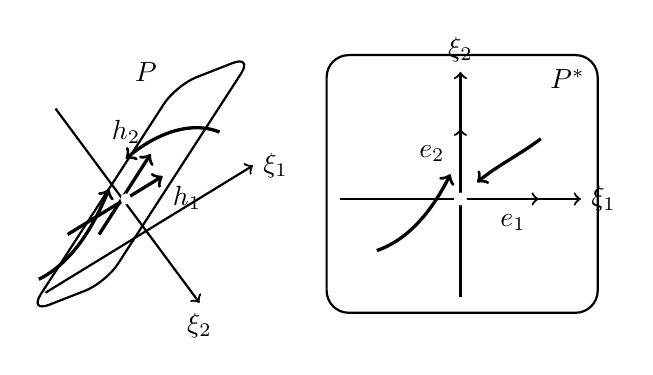
\begin{tikzpicture}[x=0.85cm,y=0.85cm,thick]
  % Oblique plane P and its eigenbasis.
  \draw[rounded corners=8pt] (-4.0,-1.65)--(-1.8,1.75)--(-0.65,2.2)--(-2.85,-1.2)--cycle;
  \coordinate (O) at (-2.55,0.05);
  \draw[->] (-3.75,-1.35)--(-0.65,0.55) node[right] {$\xi_1$};
  \draw[->] (-3.6,1.4)--(-1.45,-1.5) node[below] {$\xi_2$};
  \draw[->,very thick] (-3.42,-0.48)--(-2.0,0.39);
  \draw[->,very thick] (-2.95,-0.48)--(-2.18,0.72);
  \node[below right] at (-2.0,0.39) {$\vect{h}_1$};
  \node[above left] at (-2.18,0.72) {$\vect{h}_2$};
  \fill[white] (O) circle (2pt);
  \node at (-2.25,1.95) {$P$};
  % Sample trajectories in the skew plane.
  \draw[->,very thick] (-3.85,-1.15) .. controls (-3.25,-0.85) and (-2.95,-0.15) .. (-2.8,0.2);
  \draw[->,very thick] (-1.15,1.05) .. controls (-1.65,1.25) and (-2.2,0.95) .. (-2.55,0.65);
  % Affine image P*: orthogonal coordinate axes and corresponding trajectories.
  \draw[rounded corners=8pt] (0.45,-1.65) rectangle (4.5,2.2);
  \draw[->] (0.65,0.05)--(4.25,0.05) node[right] {$\xi_1$};
  \draw[->] (2.45,-1.42)--(2.45,1.95) node[above] {$\xi_2$};
  \draw[->,very thick] (1.2,-0.72) .. controls (1.7,-0.55) and (2.05,-0.08) .. (2.3,0.42);
  \draw[->,very thick] (3.65,0.95) .. controls (3.35,0.72) and (3.0,0.55) .. (2.7,0.3);
  \draw[->] (2.85,0.05)--(3.62,0.05) node[midway,below=2pt] {$\vect{e}_1$};
  \draw[->] (2.45,0.36)--(2.45,1.10) node[midway,left=2pt] {$\vect{e}_2$};
  \fill[white] (2.45,0.05) circle (2.3pt);
  \node at (4.05,1.85) {$P^*$};
\end{tikzpicture}

 \caption{原书图 22：左侧相平面 \(P\) 中的斜交特征方向 \(\vect{h}_1,\vect{h}_2\) 经仿射映射变为
 右侧辅助平面 \(P^*\) 的坐标轴。右侧两条待画轨线在 \(P^*\) 中以 \((\xi_1,\xi_2)\)
 为直角坐标；参数条件是两个特征值为互异实数且都非零。}
 \label{fig:ch2-p2-22}
\end{figure}

在 \(P^*\) 中，除了式 (7) 的轨线外，还分别有由
\begin{equation}
 \xi_1=c_1e^{\lambda_1t},\qquad
 \xi_2=-c_2e^{\lambda_2t}
 \tag{8}
\end{equation}
以及
\begin{equation}
 \xi_1=-c_1e^{\lambda_1t},\qquad
 \xi_2=c_2e^{\lambda_2t}
 \tag{9}
\end{equation}
给出的轨线。式 (7) 关于横轴作镜面反射得到式 (8)；关于纵轴作镜面反射到式 (9)。因此只要画出
第一象限内的轨线，就能利用这两个反射补出整个 \(P^*\)。若 \(c_1=c_2=0\)，得到原点
平衡位置；若 \(c_2=0,c_1>0\)，点在正半横轴上运动；若 \(c_1=0,c_2>0\)，点在正半纵轴
上运动。当 \(\lambda_1<0\) 时，横轴上的点朝原点运动；当 \(\lambda_1>0\) 时，点背离
原点而向无穷远运动。纵轴同理。只要 \(c_1,c_2>0\)，第一象限内的点不会越出象限边界，
因为两个坐标的指数因子都保持正号。

\subsection*{结点和鞍点}
\addcontentsline{toc}{subsection}{结点和鞍点}

\begin{sourceitem}{命题 (A)}
设 \(\lambda_1,\lambda_2\) 都非零且同号，并按绝对值大小编号，使
\begin{equation}
 |\lambda_1|<|\lambda_2|.
 \tag{10}
\end{equation}
若
\[
 \lambda_1<0,\qquad\lambda_2<0,
\]
则相图称为稳定结点；若
\[
 \lambda_1>0,\qquad\lambda_2>0,
\]
则称为不稳定结点。
\end{sourceitem}

以稳定结点为例。沿正半横轴的解为
\(\vect{\xi}(t)=(c_1e^{\lambda_1t},0)\)，沿正半纵轴的解为
\((0,c_2e^{\lambda_2t})\)，两者都随 \(t\) 增大而趋近原点。在第一象限内部，假设
\(c_1,c_2>0\)，则
\[
 \xi_1=c_1e^{\lambda_1t},\qquad
 \xi_2=c_2e^{\lambda_2t}.
\]
因为 \(\lambda_2\) 更负，纵坐标衰减更快，所以曲线在原点处与横轴相切；当
\(t\to-\infty\) 时，两个坐标都增大，但纵坐标增长更快，因此远处的运动方向更偏向纵轴。
把第一象限的曲线经平面反射平移，得到全平面图，即图 23(a)。若把两个指数同时反向，
轨线形状不变而运动方向反转，得到不稳定结点，见图 23(b)。

\begin{figure}[H]
 \centering
 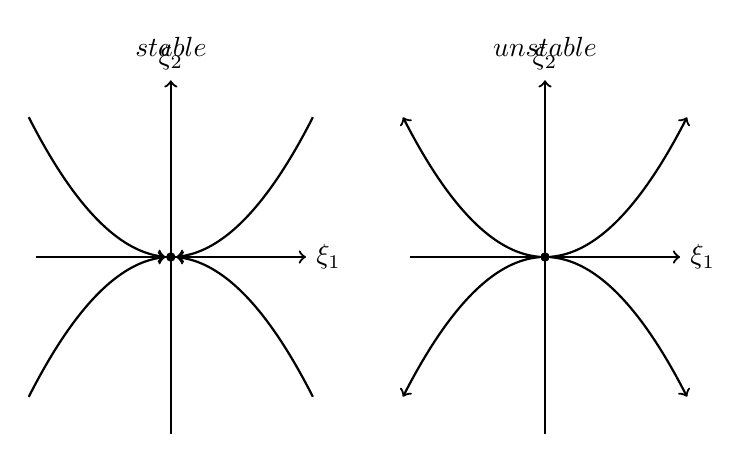
\begin{tikzpicture}[x=0.88cm,y=0.88cm,thick]
  \foreach \cx/\title in {-2.7/stable,2.7/unstable} {
    \draw[->] (\cx-1.95,0)--(\cx+1.95,0) node[right] {$\xi_1$};
    \draw[->] (\cx,-2.55)--(\cx,2.55) node[above] {$\xi_2$};
    \node[above] at (\cx,2.75) {$\title$};
    \fill (\cx,0) circle (1.7pt);
  }
  % Curves are tangent to the slow horizontal eigendirection at the node.
  \foreach \sgnx in {-1,1} {\foreach \sgny in {-1,1} {
    \draw[->] plot[domain=2.05:0.08,samples=65,variable=\s]
      ({-2.7+\sgnx*\s},{\sgny*0.48*\s*\s});
    \draw[->] plot[domain=0.08:2.05,samples=65,variable=\s]
      ({2.7+\sgnx*\s},{\sgny*0.48*\s*\s});
  }}
\end{tikzpicture}

 \caption{原书图 23：辅助平面 \(P^*\) 中的结点。两轴为特征方向；两幅图都满足
 \(|\lambda_1|<|\lambda_2|\) 且特征值同号。左图 \(\lambda_1,\lambda_2<0\)，箭头
 指向原点，是稳定结点；右图 \(\lambda_1,\lambda_2>0\)，箭头背离原点，是不稳定结点。
 曲线在原点处切于横轴，说明衰减较慢的 \(\lambda_1\) 方向占主导。}
 \label{fig:ch2-p2-23}
\end{figure}

\begin{sourceitem}{命题 (B)}
若 \(\lambda_1,\lambda_2\) 异号，则两类坐标一个衰减、一个增长。为确定起见设
\begin{equation}
 \lambda_1<0<\lambda_2.
 \tag{11}
\end{equation}
沿正半横轴的解走向原点，而沿正半纵轴的解离开原点。第一象限内的轨线是双曲线型曲线：
沿稳定方向 \(\xi_2=0\) 趋近原点，沿不稳定方向 \(\xi_1=0\) 离开原点。这个相图称为
鞍点。
\end{sourceitem}

辅助平面的标准图形即图 24。

\begin{figure}[H]
 \centering
 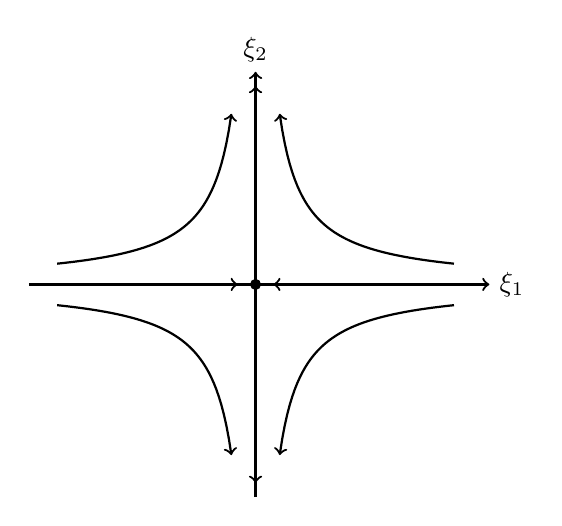
\begin{tikzpicture}[x=0.9cm,y=0.9cm,thick]
  \draw[->] (-3.2,0)--(3.3,0) node[right] {$\xi_1$};
  \draw[->] (0,-3.0)--(0,3.0) node[above] {$\xi_2$};
  % Stable horizontal and unstable vertical separatrices.
  \draw[->] (-2.8,0)--(-0.25,0); \draw[->] (2.8,0)--(0.25,0);
  \draw[->] (0,0.25)--(0,2.8); \draw[->] (0,-0.25)--(0,-2.8);
  % Hyperbolas: forward motion goes from the stable direction toward the unstable one.
  \foreach \sx in {-1,1} {\foreach \sy in {-1,1} {
    \draw[->] plot[domain=2.8:0.34,samples=70,variable=\s]
      ({\sx*\s},{\sy*0.82/\s});
  }}
  \fill (0,0) circle (2pt);
\end{tikzpicture}

 \caption{原书图 24：\(P^*\) 中的鞍点，参数条件为
 \(\lambda_1<0<\lambda_2\)。横轴 \(\xi_2=0\) 是稳定特征方向，箭头从左右两侧指向原点；
 纵轴 \(\xi_1=0\) 是不稳定特征方向，箭头从原点向外。双曲线型轨线先靠近一条特征方向，
 再转向另一条。}
 \label{fig:ch2-p2-24}
\end{figure}

图 23 与图 24 都是辅助平面 \(P^*\) 中的标准图。回到原相平面 \(P\) 时，特征向量的夹角
和长度会改变图形，所以结点可能看起来倾斜，鞍点的两条渐近特征线也未必垂直。图 25、26
给出这种仿射变形：轨线的拓扑类型不变，但弯曲程度和夹角会随 \(\vect{h}_1,\vect{h}_2\) 改变。尤其当
两个特征向量接近共线时，标准图形在 \(P\) 中会被拉得很窄，不能只凭视觉角度判断矩阵结构。

\begin{figure}[H]
 \centering
 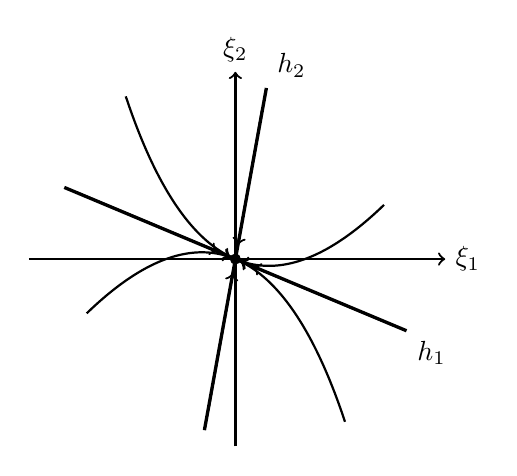
\begin{tikzpicture}[x=0.82cm,y=0.82cm,thick]
  % Stable node in a skew eigenbasis; h1 is the slow direction.
  \draw[->] (-3.2,0)--(3.25,0) node[right] {$\xi_1$};
  \draw[->] (0,-2.9)--(0,2.9) node[above] {$\xi_2$};
  \draw[very thick] (-2.65,1.11)--(2.65,-1.11) node[below right] {$\vect{h}_1$};
  \draw[very thick] (-0.48,-2.65)--(0.48,2.65) node[above right] {$\vect{h}_2$};
  \draw[->] (-2.45,1.03)--(-0.28,0.12); \draw[->] (2.45,-1.03)--(0.28,-0.12);
  \draw[->] (-0.42,-2.35)--(-0.04,-0.22); \draw[->] (0.42,2.35)--(0.04,0.22);
  % Plot v = C u^2 in eigen-coordinates, then shear it into the physical plane.
  \foreach \su in {-1,1} {\foreach \sv in {-1,1} {
    \draw[->] plot[domain=2.0:0.08,samples=65,variable=\s]
      ({\su*\s+0.18*\sv*0.42*\s*\s},{-0.42*\su*\s+\sv*0.42*\s*\s});
  }}
  \fill (0,0) circle (2pt);
\end{tikzpicture}

 \caption{原书图 25：相平面 \(P\) 中的稳定结点，坐标轴是特征方向
 \(\xi_1,\xi_2\) 的像。参数为 \(\lambda_1,\lambda_2<0\)，两个特征方向不垂直；
 轨线在原点附近偏向衰减较慢的特征方向。}
 \label{fig:ch2-p2-25}
\end{figure}

\begin{figure}[H]
 \centering
 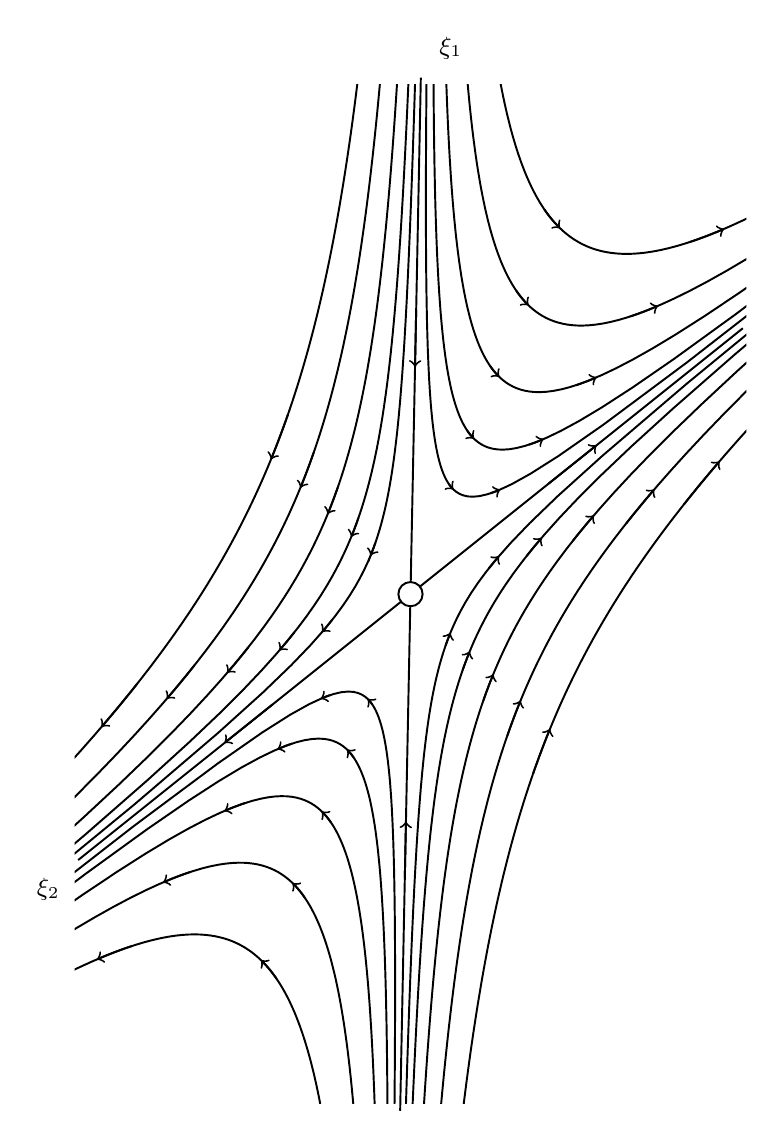
\begin{tikzpicture}[scale=2.5729,font=\small,x=0.85cm,y=0.85cm,line width=0.7pt]
  % Saddle: u'=-u, v'=v; h_1=(0.02,1), h_2=(-1,-0.8).
  % Thus x=0.02u-v, y=u-0.8v and u*v is constant along each orbit.
  \begin{scope}
    \clip (-1.95,-2.96) rectangle (1.95,2.96);
    \foreach \su in {-1,1} {
      \foreach \sv in {-1,1} {
        \foreach \k in {0.10,0.22,0.43,0.76,1.22} {
          \draw plot[domain=0.035:6,samples=220,variable=\s]
            ({0.02*\su*\s-\sv*\k/\s},
             {\su*\s-0.8*\sv*\k/\s});
          \foreach \m in {0.65,1.40} {
            \draw[->] plot[domain={1.06*\m*sqrt(\k)}:{0.94*\m*sqrt(\k)},
              samples=9,variable=\s]
              ({0.02*\su*\s-\sv*\k/\s},
               {\su*\s-0.8*\sv*\k/\s});
          }
        }
      }
    }
  \end{scope}
  \draw (-0.060,-3)--(0.060,3);
  \draw (-1.93,-1.544)--(1.93,1.544);
  \foreach \sgn in {-1,1} {
    \draw[->] ({0.02*1.65*\sgn},{1.65*\sgn})
      --({0.02*1.32*\sgn},{1.32*\sgn});
    \draw[->] ({0.80*\sgn},{0.64*\sgn})
      --({1.08*\sgn},{0.864*\sgn});
  }
  \fill[white] (0,0) circle (1.7pt);
  \draw (0,0) circle (1.7pt);
  \node[above right=3pt] at (0.060,3) {$\xi_1$};
  \node[below left=3pt] at (-1.93,-1.544) {$\xi_2$};
\end{tikzpicture}

 \caption{原书图 26：相平面 \(P\) 中的鞍点，坐标轴是特征方向
 \(\xi_1,\xi_2\) 的像。参数为 \(\lambda_1<0<\lambda_2\)，两条特征直线不垂直；
 箭头沿稳定特征方向趋近原点，并沿不稳定特征方向离开原点。}
 \label{fig:ch2-p2-26}
\end{figure}

\subsection*{焦点和中心}
\addcontentsline{toc}{subsection}{焦点和中心}

\begin{sourceitem}{命题 (C)}
现在考察矩阵有一对非实复共轭特征值的情形。写成
\begin{equation}
 \lambda=\mu+i\nu,\qquad
 \overline\lambda=\mu-i\nu,\qquad \nu\neq0.
 \tag{12}
\end{equation}
特征向量也可以选成共轭
\(\vect{h}\) 与 \(\overline{\vect{h}}\)。把
\[
 \vect{h}=\frac12(\vect{h}_1-i\vect{h}_2)
\]
中的 \(\vect{h}_1,\vect{h}_2\) 取为实向量；可以证明 \(\vect{h}_1,\vect{h}_2\) 线性无关。若它们线性相关，则 \(\vect{h}\)
与 \(\overline{\vect{h}}\) 也线性相关，这与复特征向量不属于同一个一维实方向相矛盾。因此
\((\vect{h}_1,\vect{h}_2)\) 可以作为实相平面 \(P\) 的一组基。

任一实解写成
\begin{equation}
 \vect{x}=c\,\vect{h} e^{\lambda t}
  +\overline c\,\overline{\vect{h}} e^{\overline\lambda t},
 \tag{13}
\end{equation}
其中 \(c\) 是复常数。令
\[
 \zeta=\xi_1+i\xi_2,\qquad
 \xi_1+i\xi_2=c e^{\lambda t}.
\]
于是
\[
 \vect{x}=\xi_1\vect{h}_1+\xi_2\vect{h}_2.
\]
把相平面 \(P\) 仿射映射到变量 \(\zeta\) 的辅助平面 \(P^*\)，使 \(\vect{h}_1\) 的端点变到
\(1\)，使 \(\vect{h}_2\) 的端点变到 \(i\)。则 \(\xi_1\vect{h}_1+\xi_2\vect{h}_2\) 对应
\(\xi_1+i\xi_2=\zeta\)，相轨线满足
\begin{equation}
 \zeta(t)=c e^{\lambda t}.
 \tag{14}
\end{equation}

把式 (14) 写成极坐标。令
\[
 \zeta=\rho e^{i\varphi},\qquad
 c=Re^{i\alpha}.
\]
则
\begin{equation}
 \rho(t)=Re^{\mu t},\qquad
 \varphi(t)=\nu t+\alpha.
 \tag{15}
\end{equation}
当 \(\mu\neq0\) 时，\(P^*\) 中每条轨线都是对数螺线；原相平面 \(P\) 中经仿射变形后的
对应图形称为焦点。若 \(\mu<0\)，当 \(t\) 增大时点沿螺线渐近地趋向原点，称为稳定焦点，
见图 27(a)。若 \(\mu>0\)，点离开原点而趋于无穷，称为不稳定焦点，见图 27(b)。

\begin{figure}[H]
 \centering
 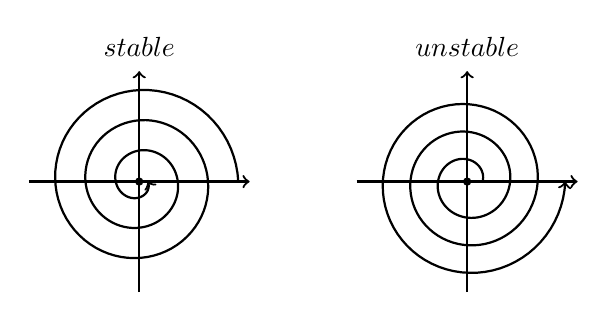
\begin{tikzpicture}[x=0.85cm,y=0.85cm,thick]
  \foreach \cx/\sgn/\title in {-2.45/-1/stable,2.45/1/unstable} {
    \draw[->] (\cx-1.65,0)--(\cx+1.65,0); \draw[->] (\cx,-1.65)--(\cx,1.65);
    \node[above] at (\cx,1.72) {$\title$}; \fill (\cx,0) circle (1.5pt);
  }
  \draw[->] plot[domain=0:1080,samples=220,variable=\t] ({-2.45+1.48*(1-\t/1180)*cos(\t)},{1.48*(1-\t/1180)*sin(\t)});
  \draw[->] plot[domain=0:1080,samples=220,variable=\t] ({2.45+(0.23+0.00115*\t)*cos(\t)},{(0.23+0.00115*\t)*sin(\t)});
\end{tikzpicture}

 \caption{原书图 27：辅助平面 \(P^*\) 中的焦点。横轴为 \(\xi_1\)，纵轴为
 \(\xi_2\)，\(\lambda=\mu\pm i\nu\) 且 \(\nu\neq0\)。左图 \(\mu<0\)，螺线随
 \(t\) 增大而向原点收紧，是稳定焦点；右图 \(\mu>0\)，螺线向外扩展，是不稳定焦点。}
 \label{fig:ch2-p2-27}
\end{figure}

若 \(\mu=0\)，则 \(\rho(t)=R\) 为常数，\(\varphi(t)=\nu t+\alpha\) 线性变化。除平衡
位置 \((0,0)\) 外，每条轨线都是闭圆；这样的相图称为中心，见图 28。中心不是
稳定焦点或渐近稳定平衡位置：解不趋近原点，只是周期地绕行。
\end{sourceitem}

\begin{figure}[H]
 \centering
 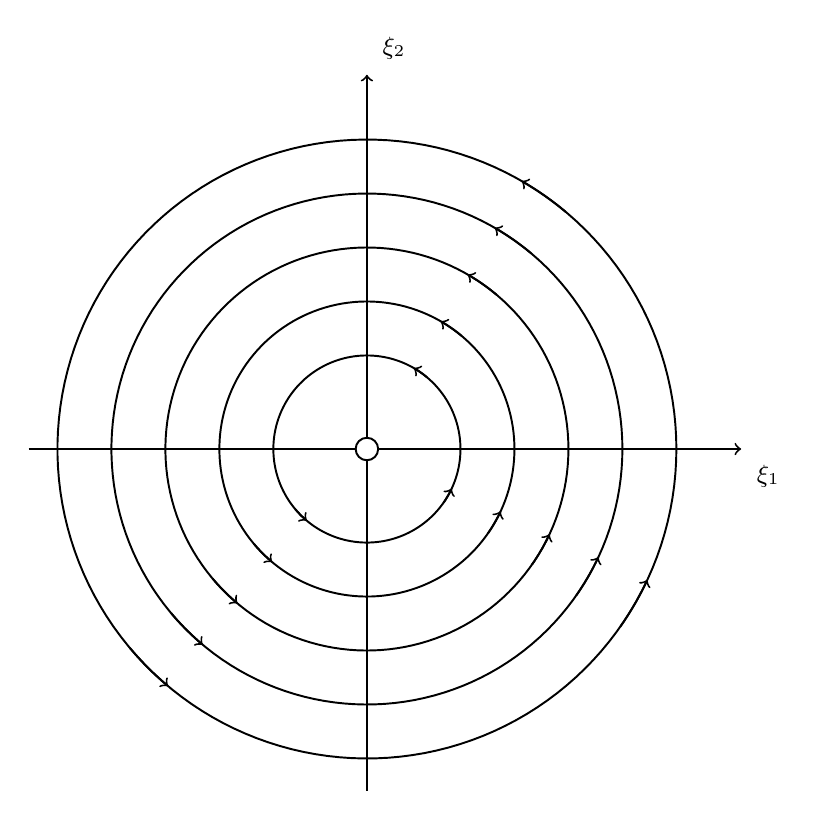
\begin{tikzpicture}[scale=2.5390,font=\small,x=0.9cm,y=0.9cm,line width=0.7pt]
  % xi_1'=-xi_2, xi_2'=xi_1: concentric counterclockwise periodic orbits.
  \foreach \r in {0.52,0.82,1.12,1.42,1.72} {
    \draw plot[domain=0:360,samples=160,variable=\a]
      ({\r*cos(\a)},{\r*sin(\a)})--cycle;
    \foreach \b in {55,225,330} {
      \draw[->] plot[domain={\b-5}:{\b+5},samples=9,variable=\a]
        ({\r*cos(\a)},{\r*sin(\a)});
    }
  }
  \draw[->] (-1.88,0)--(2.08,0);
  \draw[->] (0,-1.90)--(0,2.08);
  \fill[white] (0,0) circle (1.6pt);
  \draw (0,0) circle (1.6pt);
  \node[below right=2pt] at (2.08,0) {$\xi_1$};
  \node[above right=2pt] at (0,2.08) {$\xi_2$};
\end{tikzpicture}

 \caption{原书图 28：辅助平面 \(P^*\) 中的中心，横轴为 \(\xi_1\)、纵轴为
 \(\xi_2\)，参数条件是 \(\mu=0,\nu\neq0\)。所有非零轨线都是以原点为圆心的闭环，
 箭头方向由 \(\nu\) 的符号决定；这里每圈半径由初值 \(|c|\) 保持不变。}
 \label{fig:ch2-p2-28}
\end{figure}

图 27、28 给出 \(P^*\) 中的标准图形。回到 \(P\) 后，圆和螺线被仿射地拉成椭圆、螺线形
椭圆。图 29、30 说明这种变形：中心的同心圆可以变成同心椭圆，焦点的螺线也可以被拉斜，
但闭合与趋近原点的性质不变。

\begin{figure}[H]
 \centering
 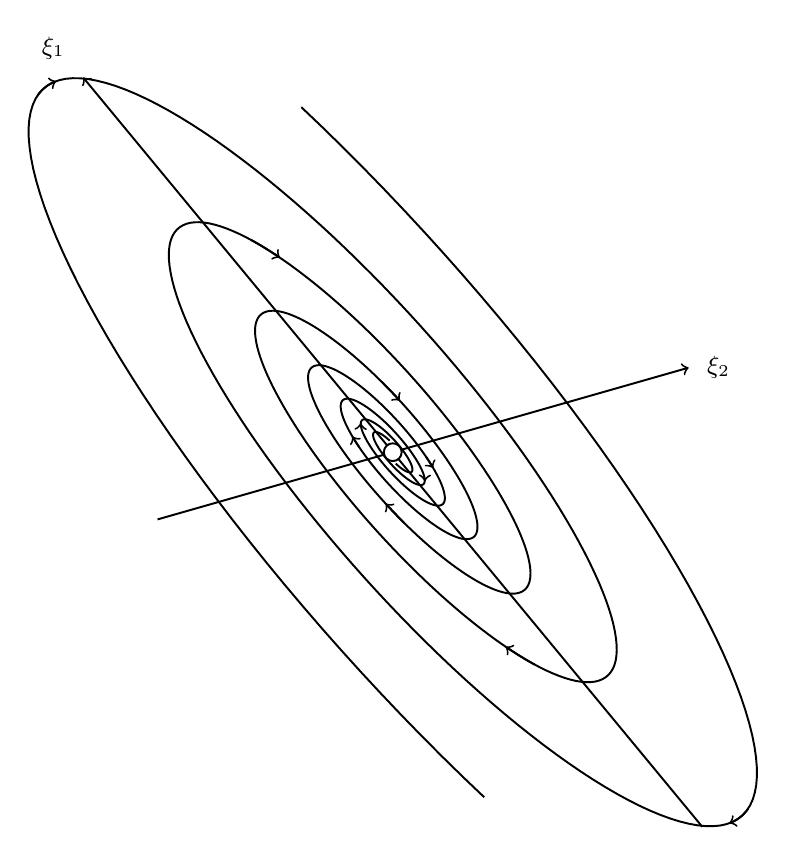
\begin{tikzpicture}[scale=2.1413,font=\small,x=0.9cm,y=0.9cm,line width=0.7pt]
  % Two centrally inverted stable logarithmic spirals under one affine map.
  % P=[(-0.95,1.15)^T,(0.42,0.12)^T], rho=3 exp(-0.0027(a-55)).
  \foreach \sgn in {-1,1} {
    \draw plot[domain=55:1315,samples=500,variable=\a]
      ({\sgn*3*exp(-0.0027*(\a-55))*(-0.95*cos(\a)+0.42*sin(\a))},
       {\sgn*3*exp(-0.0027*(\a-55))*(1.15*cos(\a)+0.12*sin(\a))});
    \foreach \j in {110,330,550,770,990} {
      \draw[->] plot[domain={55+\j-5}:{55+\j+5},samples=9,variable=\a]
        ({\sgn*3*exp(-0.0027*(\a-55))*(-0.95*cos(\a)+0.42*sin(\a))},
         {\sgn*3*exp(-0.0027*(\a-55))*(1.15*cos(\a)+0.12*sin(\a))});
    }
  }
  % Original coordinate images only: positive xi_1 is NW, positive xi_2 is NE.
  \draw[->] (2.04,-2.469)--(-2.04,2.469);
  \draw[->] (-1.55,-0.443)--(1.95,0.557);
  \fill[white] (0,0) circle (1.5pt);
  \draw (0,0) circle (1.5pt);
  \node[above left=3pt] at (-2.04,2.469) {$\xi_1$};
  \node[right=3pt] at (1.95,0.557) {$\xi_2$};
\end{tikzpicture}

 \caption{原书图 29：相平面 \(P\) 中由焦点经仿射变形得到的稳定螺旋。斜轴标出
 \(\xi_1,\xi_2\) 的像；参数为 \(\mu<0,\nu\neq0\)，沿轨线的箭头随 \(t\) 增大而向
 原点收紧。}
 \label{fig:ch2-p2-29}
\end{figure}

\begin{figure}[H]
 \centering
 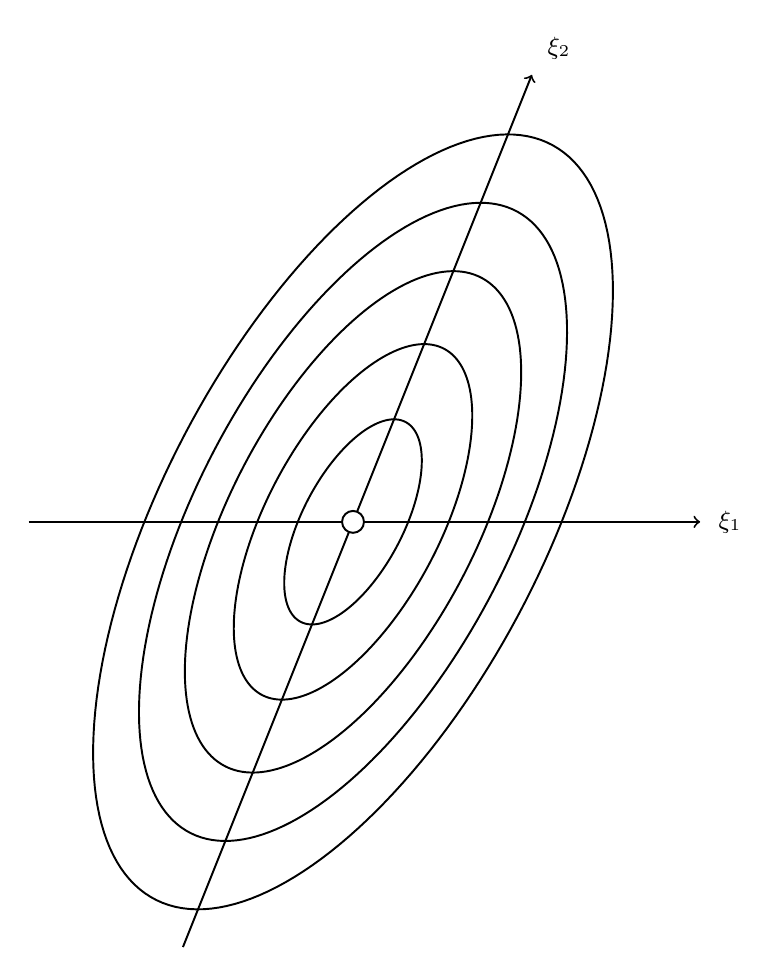
\begin{tikzpicture}[scale=2.4742,font=\small,x=0.9cm,y=0.9cm,line width=0.7pt]
  % Affine image of u'=-v, v'=u under P=[(0.70,0)^T,(0.52,1.30)^T].
  % The source shows closed orbits without flow arrows.
  \foreach \r in {0.45,0.78,1.10,1.40,1.70} {
    \draw plot[domain=0:360,samples=180,variable=\a]
      ({\r*(0.70*cos(\a)+0.52*sin(\a))},{1.30*\r*sin(\a)})--cycle;
  }
  \draw[->] (-1.85,0)--(1.98,0);
  \draw[->] (-0.97,-2.425)--(1.02,2.55);
  \fill[white] (0,0) circle (1.6pt);
  \draw (0,0) circle (1.6pt);
  \node[right=3pt] at (1.98,0) {$\xi_1$};
  \node[above right=2pt] at (1.02,2.55) {$\xi_2$};
\end{tikzpicture}

 \caption{原书图 30：相平面 \(P\) 中的中心经仿射变形得到的同心椭圆族。斜轴标出
 \(\xi_1,\xi_2\) 的像；参数为 \(\mu=0,\nu\neq0\)，每个椭圆都是闭轨线，运动方向由
 \(\nu\) 的符号决定。}
 \label{fig:ch2-p2-30}
\end{figure}

以上讨论的是非退化情形：\(\lambda_1,\lambda_2\) 不相等且都不为零。矩阵元素作足够小的
扰动时，结点、鞍点和焦点的基本相图通常保持不变；中心是例外。中心条件
\(\operatorname{tr}\mat{A}=0,\det \mat{A}>0\) 只是一个等式条件，微扰可能使实部变为负或正，于是
中心分裂成稳定焦点或不稳定焦点。这就是中心的结构不稳定性。其他退化情形，即重根或至少
一个零特征值，将在下面例题 1 和例题 3 中讨论。

\subsection*{例题}

\paragraph{例 1：退化结点.}
设方程组 (2) 的矩阵 \(\mat{A}\) 只有一个特征值 \(\lambda\)。二重特征值并
不自动意味着矩阵可对角化，因此有两种本质上不同的情形。以下用 \(\mat{A}\) 同时表示矩阵和它
所定义的线性变换。

\medskip
\noindent\textbf{情形 I.}
相平面 \(P\) 中存在由两个特征向量组成的基 \(\vect{h}_1,\vect{h}_2\)，使
\begin{equation}
 \mat{A}\vect{h}_1=\lambda \vect{h}_1,\qquad
 \mat{A}\vect{h}_2=\lambda \vect{h}_2.
 \tag{16}
\end{equation}
这等价于 \(\mat{A}=\lambda \mat{I}\) 在其特征基下可对角化，因而几何重数等于二。

\medskip
\noindent\textbf{情形 II.}
相平面中存在一组基 \(\vect{h}_1,\vect{h}_2\)，使
\begin{equation}
 \mat{A}\vect{h}_1=\lambda \vect{h}_1,\qquad
 \mat{A}\vect{h}_2=\lambda \vect{h}_2+\vect{h}_1.
 \tag{17}
\end{equation}
这时 \(\vect{h}_2\) 是二级广义特征向量，\((\vect{h}_1,\vect{h}_2)\) 是一条长度为一的 Jordan 链。

一般 Jordan 标准形定理直接保证两种基至少有一种存在。这里也可以直接验证。先取
\(\vect{h}_1\neq\vect{0}\) 为特征向量，再取任意与 \(\vect{h}_1\) 不共线的 \(\vect{h}_2\)。因为
\(\vect{h}_1,\vect{h}_2\) 构成基，可写
\[
 \mat{A}\vect{h}_2=a \vect{h}_1+\mu \vect{h}_2.
\]
在这组基下，变换矩阵为
\[
 \begin{pmatrix}
  \lambda&a\\
  0&\mu
 \end{pmatrix}.
\]
它的特征值为 \(\lambda,\mu\)，而根据假设只有唯一特征值 \(\lambda\)，所以
\(\mu=\lambda\)。若 \(a=0\)，就是情形 I。若 \(a\neq0\)，把 \(\vect{h}_1\) 换成
\(a \vect{h}_1\)；这个向量仍属于同一特征空间，并且
\[
 \mat{A} \vect{h}_2=\lambda \vect{h}_2+a \vect{h}_1
 =\lambda \vect{h}_2+(a \vect{h}_1),
\]
于是得到情形 II 的关系式 (17)。

在情形 I 中，通解可以直接写成
\begin{equation}
 \vect{x}(t)=c_1\vect{h}_1e^{\lambda t}+c_2\vect{h}_2e^{\lambda t}
 =\vect{x}_0e^{\lambda t}.
 \tag{18}
\end{equation}
只要 \(\vect{x}_0\neq\vect{0}\)，\(\lambda\neq0\) 时每个解都沿过原点、方向为 \(\vect{x}_0\) 的半射线
运动。\(\lambda<0\) 时朝原点运动，\(\lambda>0\) 时离开原点。每条由初值决定的射线本身
是一条轨线；与通常的稳定结点不同，这里没有另一条趋于较慢的特征方向，而是所有方向都以
相同指数速率伸缩。

\begin{figure}[H]
 \centering
 \begin{tikzpicture}[scale=1.7587,font=\small,x=.82cm,y=.82cm,line width=.65pt,>=Stealth]
  % Scalar matrices: every half-ray is a complete trajectory.
  \foreach \cx/\sense/\panel in {-2.8/in/a,2.8/out/b} {
    \begin{scope}[shift={(\cx,0)}]
      \foreach \ang in {0,22.5,...,337.5} {
        \draw ({.055*cos(\ang)},{.055*sin(\ang)})
          --({2.18*cos(\ang)},{2.18*sin(\ang)});
        \def\inward{in}
        \ifx\sense\inward
          \draw[->] ({1.55*cos(\ang)},{1.55*sin(\ang)})
            --({1.10*cos(\ang)},{1.10*sin(\ang)});
        \else
          \draw[->] ({.92*cos(\ang)},{.92*sin(\ang)})
            --({1.40*cos(\ang)},{1.40*sin(\ang)});
        \fi
      }
      \filldraw[fill=white,line width=.45pt] (0,0) circle (1.5pt);
      \node[below] at (0,-2.38) {(\panel)};
    \end{scope}
  }
\end{tikzpicture}

 \caption{原书图 31：例 1 情形 I 的二重特征值、可对角化情形。左图
 \(\lambda<0\)，沿每条从原点出发的半射线向内运动，原点为稳定退化结点，而且不出现
 螺旋项；右图 \(\lambda>0\)，方向反转，所有点向外运动。此情形在二维中正是
 \(\mat{A}=\lambda \mat{I}\)；图中所有半射线都是轨线。}
 \label{fig:ch2-p2-31}
\end{figure}

在情形 II 中，任意解都可写成
\begin{equation}
 \vect{x}(t)=c_1\vect{h}_1e^{\lambda t}
      +c_2(t\vect{h}_1+\vect{h}_2)e^{\lambda t}.
 \tag{19}
\end{equation}
把它按基 \((\vect{h}_1,\vect{h}_2)\) 展开为
\(\vect{x}=\xi_1\vect{h}_1+\xi_2\vect{h}_2\)，得到
\begin{equation}
 \xi_1(t)=(c_1+c_2t)e^{\lambda t},\qquad
 \xi_2(t)=c_2e^{\lambda t}.
 \tag{20}
\end{equation}
由于 \(\vect{h}_1,\vect{h}_2\) 可能不垂直，仿射映射把 \(P\) 送到辅助平面 \(P^*\)，并把 \(\vect{h}_1,\vect{h}_2\)
变成沿两个坐标轴的互相正交单位向量。在 \(P^*\) 中，式 (20) 给出
普通直角坐标下的轨线；回到 \(P\) 时再作仿射变形。

以下讨论 \(\lambda\neq0\)，\(\lambda=0\) 见例题 3。由于同时改变 \(c_1,c_2\) 的符号
把 \(P^*\) 中的点关于原点中心对称，并把轨线送到轨线，所以只要研究上半平面的轨线。
当 \(c_2=0,c_1\neq0\) 时，得到两条与横轴重合的轨线：正半横轴和负半横轴，两者都朝原点
运动。再取 \(c_1=0,c_2>0\)，得到
\begin{equation}
 \xi_1(t)=c_2te^{\lambda t},\qquad
 \xi_2(t)=c_2e^{\lambda t}.
 \tag{21}
\end{equation}

当 \(t=0\) 时，点在纵轴上的 \((0,c_2)\)。随着 \(t\) 从零增大，纵坐标以指数速度下降，
而横坐标 \(c_2te^{\lambda t}\) 先向右、随后在 \(t=-1/\lambda\) 处转向左；但整条轨线
始终向原点弯曲，并在原点处与正横轴相切。当 \(t\) 从零减到 \(-\infty\) 时，纵坐标变得
很大，横坐标为负且绝对值增长更快，整体趋势朝向负横轴。让 \(c_2\) 取遍所有正值，这样
的轨线填满上半平面。当 \(\lambda<0\) 时，所有箭头都指向原点，称为稳定的退化结点。

\begin{figure}[H]
 \centering
 \begin{tikzpicture}[x=0.76cm,y=0.76cm,thick,>=Stealth]
  % Auxiliary Jordan coordinates: trajectories are tangent to the xi_1 axis.
  \begin{scope}[shift={(-2.35,0)}]
    \draw[thin] (-1.8,0)--(1.8,0) node[right] {$\xi_1$};
    \draw[thin] (0,-1.7)--(0,1.7) node[above] {$\xi_2$};
    \node[above] at (0,2.28) {$stable$};
    \fill (0,0) circle (1.4pt);
    % Stable flow along the eigendirection.
    \draw[->] (-1.55,0)--(-0.28,0);
    \draw[<-] (0.28,0)--(1.55,0);
    % Upper trajectories enter from the left, bend around, then approach tangent to xi_1.
    \draw[->] (-2.15,1.50).. controls (-1.55,1.70) and (0.95,0.03)..(0.16,0.03);
    \draw[->] (-1.80,1.08).. controls (-1.25,1.25) and (0.70,0.02)..(0.14,0.02);
    \draw[->] (-1.45,0.68).. controls (-0.98,0.80) and (0.48,0.01)..(0.12,0.01);
    % Lower trajectories are the reflected family.
    \draw[->] (2.15,-1.50).. controls (1.55,-1.70) and (-0.95,-0.03)..(-0.16,-0.03);
    \draw[->] (1.80,-1.08).. controls (1.25,-1.25) and (-0.70,-0.02)..(-0.14,-0.02);
    \draw[->] (1.45,-0.68).. controls (0.98,-0.80) and (-0.48,-0.01)..(-0.12,-0.01);
  \end{scope}
  \begin{scope}[shift={(2.35,0)}]
    \draw[thin] (-1.8,0)--(1.8,0) node[right] {$\xi_1$};
    \draw[thin] (0,-1.7)--(0,1.7) node[above] {$\xi_2$};
    \node[above] at (0,2.28) {$unstable$};
    \fill (0,0) circle (1.4pt);
    % Reverse every arrow for the unstable case.
    \draw[<-] (-1.55,0)--(-0.28,0);
    \draw[->] (0.28,0)--(1.55,0);
    \draw[<-] (-2.15,1.50).. controls (-1.55,1.70) and (0.95,0.03)..(0.16,0.03);
    \draw[<-] (-1.80,1.08).. controls (-1.25,1.25) and (0.70,0.02)..(0.14,0.02);
    \draw[<-] (-1.45,0.68).. controls (-0.98,0.80) and (0.48,0.01)..(0.12,0.01);
    \draw[<-] (2.15,-1.50).. controls (1.55,-1.70) and (-0.95,-0.03)..(-0.16,-0.03);
    \draw[<-] (1.80,-1.08).. controls (1.25,-1.25) and (-0.70,-0.02)..(-0.14,-0.02);
    \draw[<-] (1.45,-0.68).. controls (0.98,-0.80) and (-0.48,-0.01)..(-0.12,-0.01);
  \end{scope}
\end{tikzpicture}

 \caption{原书图 32：Jordan 链基下辅助平面 \(P^*\) 的退化结点。坐标轴就是
 \((\vect{h}_1,\vect{h}_2)\) 的像。左图 \(\lambda<0\)，轨线在原点与横轴相切，运动向内，是稳定
 退化结点；右图 \(\lambda>0\)，运动向外，是不稳定退化结点。两幅图都对应二重特征值且
 只有一个独立特征向量。}
 \label{fig:ch2-p2-32}
\end{figure}

若 \(\lambda>0\)，把上面的图形关于纵轴作镜面反射并反转时间方向，就得到不稳定退化结点，
见图 32(b)。图 33(a),(b) 回到原相平面 \(P\)，显示非正交特征基造成的倾斜变形。相切的
方向仍然是唯一的特征直线 \(\vect{h}_1\)；另一条 Jordan 方向的像 \(\vect{h}_2\) 只决定曲线从哪一侧
接入。

\begin{figure}[H]
 \centering
 \begin{tikzpicture}[scale=1.1900,font=\small,line width=.65pt,>=Stealth]
  % The two original panels use different oblique bases.  Each is a
  % linear image of the exact Jordan portrait of Figure 32.
  \begin{scope}[shift={(-3.0,0)},x={(.58cm,.92cm)},y={(-.35cm,.74cm)}]
    \begin{scope}
      \clip (-2.55,-2.25)--(2.55,-2.25)--(2.55,2.25)--(-2.55,2.25)--cycle;
      \foreach \a in {.55,1.05,1.60} {
        \foreach \sgn in {-1,1} {
          \draw plot[domain=-1.5:8,samples=190,variable=\t]
            ({\sgn*2.7*\a*\t*exp(-\t)},{\sgn*\a*exp(-\t)});
          \foreach \ta/\tb in {-.28/-.12,.65/.82} {
            \draw[->] plot[domain=\ta:\tb,samples=12,variable=\t]
              ({\sgn*2.7*\a*\t*exp(-\t)},{\sgn*\a*exp(-\t)});
          }
        }
      }
    \end{scope}
    \draw[line width=.45pt] (-2.70,0)--(2.70,0)
      node[above right,xshift=2pt] {$\xi_1$};
    \draw[line width=.45pt] (0,-2.30)--(0,2.30)
      node[above left,xshift=-2pt] {$\xi_2$};
    \draw[->] (-2.2,0)--(-1.75,0);
    \draw[->] (2.2,0)--(1.75,0);
    \filldraw[fill=white,line width=.45pt] (0,0) circle (1.5pt);
  \end{scope}
  \node[below] at (-3.0,-2.95) {(a)};
  \begin{scope}[shift={(3.0,0)},x={(.78cm,.78cm)},y={(-1.20cm,0cm)}]
    \begin{scope}
      \clip (-2.55,-2.25)--(2.55,-2.25)--(2.55,2.25)--(-2.55,2.25)--cycle;
      \foreach \a in {.55,1.05,1.60} {
        \foreach \sgn in {-1,1} {
          \draw plot[domain=-1.5:8,samples=190,variable=\t]
            ({-\sgn*2.7*\a*\t*exp(-\t)},{\sgn*\a*exp(-\t)});
          \foreach \ta/\tb in {-.28/-.12,.65/.82} {
            \draw[<-] plot[domain=\ta:\tb,samples=12,variable=\t]
              ({-\sgn*2.7*\a*\t*exp(-\t)},{\sgn*\a*exp(-\t)});
          }
        }
      }
    \end{scope}
    \draw[line width=.45pt] (-2.70,0)--(2.70,0)
      node[above right,xshift=2pt] {$\xi_1$};
    \draw[line width=.45pt] (0,-2.30)--(0,2.30)
      node[left,xshift=-2pt] {$\xi_2$};
    \draw[->] (-1.75,0)--(-2.2,0);
    \draw[->] (1.75,0)--(2.2,0);
    \filldraw[fill=white,line width=.45pt] (0,0) circle (1.5pt);
  \end{scope}
  \node[below] at (3.0,-2.95) {(b)};
\end{tikzpicture}

 \caption{原书图 33：原相平面 \(P\) 中的退化结点。与图 32 相比，坐标轴不再正交，曲线被
 仿射拉斜，但两个特征方向 \(\vect{h}_1,\vect{h}_2\) 仍然保留；轨线在原点附近仍切于特征方向
 \(\vect{h}_1\)。左、右两个图形对应稳定和不稳定两个时间方向。}
 \label{fig:ch2-p2-33}
\end{figure}

\paragraph{例 2：二阶常系数线性齐次方程.}
考虑标量方程
\begin{equation}
 \ddot x+a\dot x+bx=0,
 \qquad a,b\in\R,
 \tag{22}
\end{equation}
其中 \(\dot x\) 表示对时间的导数。按第~\S4 的方法引入状态变量 \((x,\dot x)\)，可写成
标准方程组
\begin{equation}
 \dot x=y,\qquad
 \dot y=-bx-ay.
 \tag{23}
\end{equation}
把 \((x,y)\) 平面看成原方程的相平面。直接计算可知，方程组 (23)
的系数矩阵特征多项式为
\begin{equation}
 p^2+ap+b.
 \tag{24}
\end{equation}
它正好是原二阶方程的特征多项式。因此前面关于相平面的结点、鞍点、焦点和中心结论都可以
直接用于二阶方程。

若式 (24) 的根为复数，则相平面出现焦点或中心。下面讨论两根非零、
互不相同且为实数的情形。设 \(\lambda\) 是根，\(\vect{h}=(h^1,h^2)\neq\vect{0}\) 是对应特征向量。
由方程组 (23) 的形式，
\[
 \lambda h^1=h^2.
\]
因此特征方向由
\begin{equation}
 y=\lambda x
 \tag{25}
\end{equation}
确定；这条直线称为特征直线。这里第一坐标是位移，第二坐标是速度；图中的横轴标为
\(x\)，纵轴标为 \(\dot x\)，两者都是同一标量函数的相位坐标。

若 \(\lambda_1,\lambda_2<0\)，就有稳定结点，见命题 (A)。两条特征直线都经过第二、
第四象限；在原点附近，轨线切于靠近横轴的那条特征直线。其原因是该方向对应的
\(|\lambda|\) 较小，指数衰减较慢，故成为进入原点时的主导方向。图 34 给出这一情形。

\begin{figure}[H]
 \centering
 \begin{tikzpicture}[x=0.8cm,y=0.8cm,thick,>=Stealth]
  \draw[->] (-4.4,0)--(4.4,0) node[right] {$x$};
  \draw[->] (0,-3.5)--(0,3.5) node[above] {$\dot x$};
  % Stable eigenlines: one slow, shallow direction and one fast, steep direction.
  \draw[very thick] (-4.0,1.4)--(4.0,-1.4);
  \draw[very thick] (-2.55,3.45)--(2.55,-3.45);
  \draw[->] (-2.65,0.93)--(-0.24,0.084);
  \draw[->] (2.65,-0.93)--(0.24,-0.084);
  \draw[->] (-1.85,2.50)--(-0.18,0.24);
  \draw[->] (1.85,-2.50)--(0.18,-0.24);
  % Distinct trajectories curve through the upper-left and lower-right sectors.
  % Each approaches the origin tangent to the slower eigendirection.
  \draw[->] (-3.75,2.95).. controls (-3.05,2.75) and (-1.05,0.42)..(-0.14,0.05);
  \draw[->] (-3.35,2.20).. controls (-2.65,2.05) and (-0.92,0.34)..(-0.14,0.05);
  \draw[->] (-3.05,1.45).. controls (-2.35,1.42) and (-0.82,0.29)..(-0.14,0.05);
  \draw[->] (3.75,-2.95).. controls (3.05,-2.75) and (1.05,-0.42)..(0.14,-0.05);
  \draw[->] (3.35,-2.20).. controls (2.65,-2.05) and (0.92,-0.34)..(0.14,-0.05);
  \draw[->] (3.05,-1.45).. controls (2.35,-1.42) and (0.82,-0.29)..(0.14,-0.05);
  \fill (0,0) circle (2pt);
\end{tikzpicture}

 \caption{原书图 34：方程 (24) 的两根皆为负实根时的稳定结点。
 横轴为位移 \(x\)，纵轴为速度 \(\dot x\)；两条斜线是满足 \(\dot x=\lambda x\) 的
 特征直线。所有箭头指向原点，轨线在原点附近切于衰减较慢的特征直线。}
 \label{fig:ch2-p2-34}
\end{figure}

若 \(\lambda_1,\lambda_2>0\)，则有拓扑上的不稳定结点。两条特征直线经过第一、第三象限，
轨线在原点附近仍切于位置较靠近横轴的那条特征直线，但箭头反向，点随时间离开原点。
见图 35。

\begin{figure}[H]
 \centering
 \begin{tikzpicture}[x=0.8cm,y=0.8cm,thick,>=Stealth]
  \draw[->] (-4.4,0)--(4.4,0) node[right] {$x$};
  \draw[->] (0,-3.5)--(0,3.5) node[above] {$\dot x$};
  % Unstable eigenlines have positive slopes.
  \draw[very thick] (-4.0,-1.4)--(4.0,1.4);
  \draw[very thick] (-2.55,-3.45)--(2.55,3.45);
  \draw[->] (0.24,0.084)--(2.65,0.93);
  \draw[->] (-0.24,-0.084)--(-2.65,-0.93);
  \draw[->] (0.18,0.24)--(1.85,2.50);
  \draw[->] (-0.18,-0.24)--(-1.85,-2.50);
  % Reverse-flow companions of the stable-node curves; all arrows leave zero.
  \draw[<-] (3.75,2.95).. controls (3.05,2.75) and (1.05,0.42)..(0.14,0.05);
  \draw[<-] (3.35,2.20).. controls (2.65,2.05) and (0.92,0.34)..(0.14,0.05);
  \draw[<-] (3.05,1.45).. controls (2.35,1.42) and (0.82,0.29)..(0.14,0.05);
  \draw[<-] (-3.75,-2.95).. controls (-3.05,-2.75) and (-1.05,-0.42)..(-0.14,-0.05);
  \draw[<-] (-3.35,-2.20).. controls (-2.65,-2.05) and (-0.92,-0.34)..(-0.14,-0.05);
  \draw[<-] (-3.05,-1.45).. controls (-2.35,-1.42) and (-0.82,-0.29)..(-0.14,-0.05);
  \fill (0,0) circle (2pt);
\end{tikzpicture}

 \caption{原书图 35：方程 (24) 的两根皆为正实根时的不稳定结点。
 横轴 \(x\)、纵轴 \(\dot x\)；两条特征直线 \(\dot x=\lambda_i x\) 均经过第一、第三
 象限，箭头由原点向外。原点附近的主导方向仍是衰减较慢（这里等价于增长较慢）的特征
 直线。}
 \label{fig:ch2-p2-35}
\end{figure}

若两根异号，则原方程为鞍点。两条特征直线中一条经过第二、第四象限，另一条经过第一、
第三象限。轨线沿稳定的特征方向接近原点，而沿不稳定方向离开原点。图 36 给出这一力学
相图；两条双曲线分支的连接方式由 \(b<0\) 和根的符号确定。

\begin{figure}[H]
 \centering
 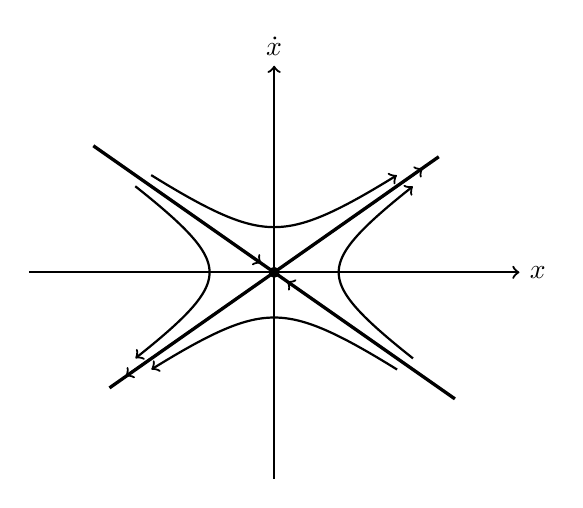
\begin{tikzpicture}[x=0.82cm,y=0.82cm,thick]
  \draw[->] (-3.8,0)--(3.8,0) node[right] {$x$};
  \draw[->] (0,-3.2)--(0,3.2) node[above] {$\dot x$};
  % Stable eigenline has negative slope; unstable eigenline has positive slope.
  \draw[very thick] (-2.8,1.96)--(2.8,-1.96);
  \draw[very thick] (-2.55,-1.79)--(2.55,1.79);
  \draw[->] (-2.5,1.75)--(-0.2,0.14); \draw[->] (2.5,-1.75)--(0.2,-0.14);
  \draw[->] (0.2,0.14)--(2.3,1.61); \draw[->] (-0.2,-0.14)--(-2.3,-1.61);
  % Hyperbolic sample orbits for one negative and one positive eigenvalue.
  \foreach \cOne/\cTwo in {0.5/0.5,0.5/-0.5,-0.5/0.5,-0.5/-0.5} {
    \draw[->] plot[domain=-2:2,samples=140,variable=\t]
      ({\cOne*exp(-0.7*\t)+\cTwo*exp(0.7*\t)},
       {-0.7*\cOne*exp(-0.7*\t)+0.7*\cTwo*exp(0.7*\t)});
  }
  \fill (0,0) circle (2pt);
\end{tikzpicture}

 \caption{原书图 36：方程 (24) 的根一正一负时的相图。横轴为
 \(x\)，纵轴为 \(\dot x\)。一条特征直线经过第二、第四象限，另一条经过第一、第三象限；
 箭头沿前者趋近原点、沿后者离开原点，故为鞍点。}
 \label{fig:ch2-p2-36}
\end{figure}

\paragraph{例 3：至少一个特征值等于零.}

\medskip
\noindent\textbf{情形 I.}
只有一个特征值等于零：
\begin{equation}
 \lambda_1\neq0,\qquad\lambda_2=0.
 \tag{26}
\end{equation}
这时解仍按式 (3) 写，其中
\begin{equation}
 \xi_1(t)=c_1e^{\lambda_1t},\qquad
 \xi_2(t)=c_2.
 \tag{27}
\end{equation}
因为 \(\xi_2=c_2\) 为常数，所有沿固定直线 \(\xi_2=\text{常数}\) 的运动都平行于
\(\xi_1\) 轴；当 \(\lambda_1<0\) 时朝直线 \(\xi_1=0\) 运动，当 \(\lambda_1>0\) 时背离
它运动。直线 \(\xi_1=0\) 上每一点都满足 \(\vect{f}(\vect{x})=\vect{0}\)，因此整条直线由平衡位置组成。
原点不再是唯一平衡位置，所以不能用孤立的结点、鞍点或焦点来称呼这一相图。图 37 给出
辅助平面中的这一结构。

\begin{figure}[H]
 \centering
 \begin{tikzpicture}[scale=2.1634,font=\small,x={(1cm,-.27cm)},y={(.68cm,.74cm)},
  line width=.65pt,>=Stealth]
  % Affine image of xi_1'=lambda_1 xi_1, xi_2'=0, lambda_1<0.
  % The whole oblique xi_2 axis consists of equilibria.
  \foreach \h in {-1.65,-1.10,-.55,.55,1.10,1.65} {
    \draw (-1.90,\h)--(1.90,\h);
    \draw[->] (-1.42,\h)--(-.78,\h);
    \draw[->] (1.42,\h)--(.78,\h);
  }
  \draw[line width=.45pt] (-2.10,0)--(2.10,0)
    node[right,xshift=3pt] {$\xi_1$};
  \draw[->,line width=.55pt] (0,-2.05)--(0,2.05)
    node[above right,xshift=2pt] {$\xi_2$};
  \draw[->] (-1.42,0)--(-.78,0);
  \draw[->] (1.42,0)--(.78,0);
  \filldraw[fill=white,line width=.45pt] (0,0) circle (1.5pt);
\end{tikzpicture}

 \caption{原书图 37：零特征值情形 I，特征值为 \(\lambda_1\neq0,\lambda_2=0\)。
 两条坐标轴为特征方向；直线 \(\xi_1=0\) 上每一点都是平衡位置。轨迹沿水平直线
 \(\xi_2=\text{常数}\) 指向或背离 \(\xi_1=0\)，方向由 \(\lambda_1\) 的符号决定。
 图示 \(\lambda_1<0\)，轨线指向平衡直线；当 \(\lambda_1>0\) 时，所有箭头反向。}
 \label{fig:ch2-p2-37}
\end{figure}

\medskip
\noindent\textbf{情形 II.}
若唯一特征值为
\begin{equation}
 \lambda_1=\lambda_2=0,
 \tag{28}
\end{equation}
则可能分别落在例题 1 的两种情形。

\emph{情形 II.1.} 见关系式 (16) 且 \(\lambda=0\)。通解
(18) 成为
\begin{equation}
 \vect{x}(t)=\vect{x}_0.
 \tag{29}
\end{equation}
这只有当方程组 (1) 的所有系数都等于零时才发生；此时相平面每一点
都是平衡位置，整个平面都是静止的，没有需要分类的轨线。

\emph{情形 II.2.} 见关系式 (17) 且 \(\lambda=0\)。通解
(19) 成为
\begin{equation}
 \xi_1(t)=c_1+c_2t,\qquad
 \xi_2(t)=c_2.
 \tag{30}
\end{equation}
沿着每一条固定直线 \(\xi_2=\text{常数}\)，运动都以常速度 \(c_2\) 进行；当 \(c_2>0\)
时向右，当 \(c_2<0\) 时向左。直线 \(\xi_2=0\) 上所有点都有 \(c_2=0\)，因此都是平衡
位置。图 38 显示这种一维平移的平行轨线族。

\begin{figure}[H]
 \centering
 \begin{tikzpicture}[scale=2.1989,font=\small,x={(.87cm,.22cm)},y={(.12cm,.74cm)},
  line width=.65pt,>=Stealth]
  % Keep the scanned oblique layout; correct its reversed flow arrows
  % according to xi_1'=xi_2, xi_2'=0 in equation (30).
  \foreach \h in {.35,.70,1.05,1.40,1.75,2.10} {
    \draw (-3.10,\h)--(3.10,\h);
    \draw (-3.10,-\h)--(3.10,-\h);
    \foreach \p in {-2.30,-.45,1.40} {
      \draw[->] (\p,\h)--({\p+.55},\h);
      \draw[<-] (\p,-\h)--({\p+.55},-\h);
    }
  }
  \draw[line width=.8pt] (-3.10,0)--(3.10,0)
    node[right,xshift=3pt] {$\xi_1$};
  \draw[line width=.45pt] (0,-2.45)--(0,2.45)
    node[above right,xshift=2pt] {$\xi_2$};
\end{tikzpicture}

 \caption{原书图 38：零特征值且矩阵不可对角化的情形。坐标轴为
 \((\xi_1,\xi_2)\) 的特征链方向；每条水平直线 \(\xi_2=\text{常数}\) 是一条轨线，
 运动匀速并沿 \(\xi_1\) 方向。直线 \(\xi_2=0\) 由平衡位置组成。与图 37 相比，这里
 没有非零指数伸缩，时间依赖是线性的。}
 \label{fig:ch2-p2-38}
\end{figure}
